\documentclass[11pt,twoside,openright]{book}

% Core packages
\usepackage[utf8]{inputenc}
\usepackage[T1]{fontenc}
\usepackage{lmodern}
\usepackage{microtype} % Typography enhancements
\usepackage{amsmath,amsfonts,amssymb,mathtools}
\usepackage{xcolor}
\usepackage{booktabs} % Professional tables
\usepackage{graphicx}
\usepackage{hyperref}
\usepackage{cleveref}

% Page layout
\usepackage[margin=1in,headheight=25pt]{geometry}
\usepackage{fancyhdr}

% Set up fancy headers and footers
\pagestyle{fancy}
\fancyhf{} % Clear all header and footer fields

% Create shorter chapter/section mark formats to prevent overlap with logo
\renewcommand{\chaptermark}[1]{\markboth{\chaptername\ \thechapter:\ #1}{}}
\renewcommand{\sectionmark}[1]{\markright{\thesection\ #1}}

% Define header contents
\fancyhead[LE]{\leftmark} % Left side of even pages: Chapter title
\fancyhead[RO]{\rightmark} % Right side of odd pages: Section title
\fancyhead[RE]{\raisebox{-0.1\height}{\hspace{1cm}% Artistic header logo for the survival analysis book
% Abstract visualization of survival concepts without borders

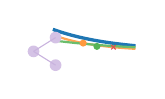
\begin{tikzpicture}[scale=0.35, baseline=(current bounding box.center)]
    % No visible background or border

    % Multiple stylized curves representing different survival functions
    \draw[very thick, primary, domain=0:3, samples=30]
        plot (\x, {0.8*exp(-\x/2.2)});

    \draw[thick, secondary!70, domain=0:3, samples=30]
        plot (\x, {0.6*exp(-\x/1.6)});

    \draw[thick, tertiary!70, domain=0:3, samples=30]
        plot (\x, {0.4*exp(-\x/3)});

    % Abstract neural network nodes (filled circles without borders)
    \node[circle, fill=quinary!40, inner sep=1.5pt] at (-0.7,0) {};
    \node[circle, fill=quinary!40, inner sep=1.5pt] at (0.1,-0.5) {};
    \node[circle, fill=quinary!40, inner sep=1.5pt] at (0.1,0.5) {};
    \draw[quinary!50, thin] (-0.7,0) -- (0.1,-0.5);
    \draw[quinary!50, thin] (-0.7,0) -- (0.1,0.5);

    % Event indicators with different patterns (smaller dots)
    \node[circle, fill=secondary!80, inner sep=0.9pt] at (1.1,0.3) {};
    \node[circle, fill=tertiary!80, inner sep=0.9pt] at (1.6,0.18) {};

    % Subtle censoring mark
    \draw[quaternary!80, thin] (2.2-0.08,0.15+0.08) -- (2.2+0.08,0.15-0.08);
    \draw[quaternary!80, thin] (2.2-0.08,0.15-0.08) -- (2.2+0.08,0.15+0.08);
\end{tikzpicture}
}} % Right side of even pages: Logo with space
\fancyhead[LO]{\raisebox{-0.1\height}{% Artistic header logo for the survival analysis book
% Abstract visualization of survival concepts without borders

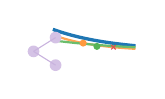
\begin{tikzpicture}[scale=0.35, baseline=(current bounding box.center)]
    % No visible background or border

    % Multiple stylized curves representing different survival functions
    \draw[very thick, primary, domain=0:3, samples=30]
        plot (\x, {0.8*exp(-\x/2.2)});

    \draw[thick, secondary!70, domain=0:3, samples=30]
        plot (\x, {0.6*exp(-\x/1.6)});

    \draw[thick, tertiary!70, domain=0:3, samples=30]
        plot (\x, {0.4*exp(-\x/3)});

    % Abstract neural network nodes (filled circles without borders)
    \node[circle, fill=quinary!40, inner sep=1.5pt] at (-0.7,0) {};
    \node[circle, fill=quinary!40, inner sep=1.5pt] at (0.1,-0.5) {};
    \node[circle, fill=quinary!40, inner sep=1.5pt] at (0.1,0.5) {};
    \draw[quinary!50, thin] (-0.7,0) -- (0.1,-0.5);
    \draw[quinary!50, thin] (-0.7,0) -- (0.1,0.5);

    % Event indicators with different patterns (smaller dots)
    \node[circle, fill=secondary!80, inner sep=0.9pt] at (1.1,0.3) {};
    \node[circle, fill=tertiary!80, inner sep=0.9pt] at (1.6,0.18) {};

    % Subtle censoring mark
    \draw[quaternary!80, thin] (2.2-0.08,0.15+0.08) -- (2.2+0.08,0.15-0.08);
    \draw[quaternary!80, thin] (2.2-0.08,0.15-0.08) -- (2.2+0.08,0.15+0.08);
\end{tikzpicture}
\hspace{1cm}}} % Left side of odd pages: Logo with space

% Define footer contents
\fancyfoot[LE,RO]{\thepage} % Page number
\fancyfoot[CE,CO]{\leftmark} % Center of footer: Chapter title instead of section
\renewcommand{\footrulewidth}{0.4pt} % Add footer line

% Create chapter style that doesn't use the fancy header
\fancypagestyle{plain}{%
  \fancyhf{} % clear all header and footer fields
  \fancyfoot[LE,RO]{\thepage} % page number
  \renewcommand{\headrulewidth}{0pt}
  \renewcommand{\footrulewidth}{0.4pt}
}

% Enhanced visualizations
\usepackage{tikz}
\usetikzlibrary{arrows.meta,positioning,shapes,shapes.geometric,decorations,patterns,fit,calc,shadows,backgrounds,math}
% Ensure the calc library is loaded for coordinate calculations
\usetikzlibrary{calc}
\usepackage{pgfplots}
\pgfplotsset{compat=newest}
\usepgfplotslibrary{fillbetween}

% Beautiful boxes
\usepackage[many]{tcolorbox}
\tcbuselibrary{skins,breakable,theorems}

% Import color scheme and box definitions
% ===================================
% COLOR SCHEME DEFINITIONS
% ===================================
% This file defines a consistent color palette for the entire book
% To use, include this file in book.tex with % ===================================
% COLOR SCHEME DEFINITIONS
% ===================================
% This file defines a consistent color palette for the entire book
% To use, include this file in book.tex with % ===================================
% COLOR SCHEME DEFINITIONS
% ===================================
% This file defines a consistent color palette for the entire book
% To use, include this file in book.tex with \input{book-sections/color-scheme.tex}

% Define primary colors
\definecolor{primary}{RGB}{31, 119, 180}       % Blue
\definecolor{secondary}{RGB}{255, 127, 14}     % Orange
\definecolor{tertiary}{RGB}{44, 160, 44}       % Green
\definecolor{quaternary}{RGB}{214, 39, 40}     % Red
\definecolor{quinary}{RGB}{148, 103, 189}      % Purple
\definecolor{senary}{RGB}{140, 86, 75}         % Brown
\definecolor{septenary}{RGB}{227, 119, 194}    % Pink
\definecolor{octonary}{RGB}{127, 127, 127}     % Gray
\definecolor{nonary}{RGB}{188, 189, 34}        % Olive
\definecolor{denary}{RGB}{23, 190, 207}        % Cyan

% Define light versions for fills and backgrounds
\definecolor{primaryLight}{RGB}{174, 199, 232}
\definecolor{secondaryLight}{RGB}{255, 187, 120}
\definecolor{tertiaryLight}{RGB}{152, 223, 138}
\definecolor{quaternaryLight}{RGB}{255, 152, 150}
\definecolor{quinaryLight}{RGB}{197, 176, 213}
\definecolor{senaryLight}{RGB}{196, 156, 148}
\definecolor{septenaryLight}{RGB}{247, 182, 210}
\definecolor{octonaryLight}{RGB}{199, 199, 199}
\definecolor{nonaryLight}{RGB}{219, 219, 141}
\definecolor{denaryLight}{RGB}{158, 218, 229}

% Define dark versions for text and lines
\definecolor{primaryDark}{RGB}{17, 63, 96}
\definecolor{secondaryDark}{RGB}{179, 89, 10}
\definecolor{tertiaryDark}{RGB}{22, 80, 22}
\definecolor{quaternaryDark}{RGB}{136, 22, 22}
\definecolor{quinaryDark}{RGB}{94, 66, 121}
\definecolor{senaryDark}{RGB}{85, 52, 45}
\definecolor{septenaryDark}{RGB}{143, 75, 122}
\definecolor{octonaryDark}{RGB}{64, 64, 64}
\definecolor{nonaryDark}{RGB}{104, 104, 18}
\definecolor{denaryDark}{RGB}{14, 115, 124}

% ===================================
% TCOLORBOX STYLES
% ===================================

% Reset tcolorbox definitions with the new colors
\newtcolorbox{definitionbox}[1][]{
    enhanced,
    colback=primaryLight!60!white,
    colframe=primary!75!black,
    fonttitle=\bfseries,
    coltitle=white,
    attach boxed title to top left={yshift=-2mm, xshift=5mm},
    boxed title style={colback=primary!75!black},
    title=Definition,
    #1
}

\newtcolorbox{equationbox}[1][]{
    enhanced,
    colback=secondaryLight!60!white,
    colframe=secondary!75!black,
    fonttitle=\bfseries,
    breakable,
    coltitle=white,
    attach boxed title to top left={yshift=-2mm, xshift=5mm},
    boxed title style={colback=secondary!75!black},
    title=Equation,
    #1
}

\newtcolorbox{examplebox}[1][]{
    enhanced,
    colback=tertiaryLight!60!white,
    colframe=tertiary!75!black,
    fonttitle=\bfseries,
    coltitle=white,
    attach boxed title to top left={yshift=-2mm, xshift=5mm},
    boxed title style={colback=tertiary!75!black},
    title=Example,
    #1
}

\newtcolorbox{notebox}[1][]{
    enhanced,
    colback=quinaryLight!60!white,
    colframe=quinary!75!black,
    fonttitle=\bfseries,
    coltitle=white,
    attach boxed title to top left={yshift=-2mm, xshift=5mm},
    boxed title style={colback=quinary!75!black},
    title=Note,
    #1
}

% ===================================
% TIKZ AND PGFPLOTS STYLES
% ===================================

% TikZ styles
\tikzset{
    concept/.style={
        draw=primary,
        fill=primaryLight,
        rounded corners,
        thick,
        align=center
    },
    process/.style={
        draw=secondary,
        fill=secondaryLight,
        rectangle,
        thick,
        align=center
    },
    decision/.style={
        draw=tertiary,
        fill=tertiaryLight,
        diamond,
        thick,
        align=center
    },
    data/.style={
        draw=quaternary,
        fill=quaternaryLight,
        cylinder,
        thick,
        align=center
    },
    note/.style={
        draw=quinary,
        fill=quinaryLight,
        cloud,
        cloud puffs=15,
        thick,
        align=center
    },
    arrow/.style={
        ->,
        >=stealth,
        thick
    }
}

% PGFPlots styles
\pgfplotscreateplotcyclelist{conceptcolors}{
    {primary, mark=*, thick, mark options={fill=primary}},
    {secondary, mark=square*, thick, mark options={fill=secondary}},
    {tertiary, mark=triangle*, thick, mark options={fill=tertiary}},
    {quaternary, mark=diamond*, thick, mark options={fill=quaternary}},
    {quinary, mark=pentagon*, thick, mark options={fill=quinary}},
    {senary, mark=*, thick, mark options={fill=senary}},
    {septenary, mark=square*, thick, mark options={fill=septenary}},
    {octonary, mark=triangle*, thick, mark options={fill=octonary}},
    {nonary, mark=diamond*, thick, mark options={fill=nonary}},
    {denary, mark=pentagon*, thick, mark options={fill=denary}}
}

% ===================================
% CONCEPT-SPECIFIC COLORS
% ===================================

% Assign consistent colors to specific concepts
% These can be used across diagrams to ensure the same concept has the same color

% Survival functions and models
\colorlet{survivalFunctionColor}{primary}
\colorlet{hazardFunctionColor}{secondary}
\colorlet{censoringColor}{quaternary}
\colorlet{kaplameierColor}{tertiary}

% Model types
\colorlet{dsmColor}{quinary}
\colorlet{mensaColor}{septenary}
\colorlet{deephitColor}{senary}

% Loss functions
\colorlet{likelihoodLossColor}{primary}
\colorlet{rankingLossColor}{secondary}
\colorlet{regressionLossColor}{tertiary}
\colorlet{classificationLossColor}{quaternary}
\colorlet{auxiliaryLossColor}{quinary}

% Events
\colorlet{event1Color}{primary}
\colorlet{event2Color}{secondary}
\colorlet{event3Color}{tertiary}
\colorlet{event4Color}{quaternary}

% Risk groups
\colorlet{lowRiskColor}{tertiary}
\colorlet{mediumRiskColor}{primary}
\colorlet{highRiskColor}{quaternary}

% ===================================
% USAGE EXAMPLES
% ===================================
%
% For tcolorbox:
% \begin{definitionbox}[title=Custom Title]
% Content
% \end{definitionbox}
%
% For TikZ:
% \begin{tikzpicture}
%   \node[concept] (a) {Concept};
%   \node[process] (b) at (2,0) {Process};
%   \draw[arrow] (a) -- (b);
% \end{tikzpicture}
%
% For PGFPlots:
% \begin{tikzpicture}
%   \begin{axis}[cycle list name=conceptcolors]
%     \addplot coordinates {(0,0) (1,1) (2,4)};
%     \addplot coordinates {(0,0) (1,2) (2,3)};
%   \end{axis}
% \end{tikzpicture}
%
% For concept-specific colors:
% \begin{tikzpicture}
%   \draw[survivalFunctionColor, thick] plot coordinates {(0,1) (1,0.8) (2,0.6)};
%   \draw[hazardFunctionColor, thick] plot coordinates {(0,0.2) (1,0.4) (2,0.6)};
% \end{tikzpicture}


% Define primary colors
\definecolor{primary}{RGB}{31, 119, 180}       % Blue
\definecolor{secondary}{RGB}{255, 127, 14}     % Orange
\definecolor{tertiary}{RGB}{44, 160, 44}       % Green
\definecolor{quaternary}{RGB}{214, 39, 40}     % Red
\definecolor{quinary}{RGB}{148, 103, 189}      % Purple
\definecolor{senary}{RGB}{140, 86, 75}         % Brown
\definecolor{septenary}{RGB}{227, 119, 194}    % Pink
\definecolor{octonary}{RGB}{127, 127, 127}     % Gray
\definecolor{nonary}{RGB}{188, 189, 34}        % Olive
\definecolor{denary}{RGB}{23, 190, 207}        % Cyan

% Define light versions for fills and backgrounds
\definecolor{primaryLight}{RGB}{174, 199, 232}
\definecolor{secondaryLight}{RGB}{255, 187, 120}
\definecolor{tertiaryLight}{RGB}{152, 223, 138}
\definecolor{quaternaryLight}{RGB}{255, 152, 150}
\definecolor{quinaryLight}{RGB}{197, 176, 213}
\definecolor{senaryLight}{RGB}{196, 156, 148}
\definecolor{septenaryLight}{RGB}{247, 182, 210}
\definecolor{octonaryLight}{RGB}{199, 199, 199}
\definecolor{nonaryLight}{RGB}{219, 219, 141}
\definecolor{denaryLight}{RGB}{158, 218, 229}

% Define dark versions for text and lines
\definecolor{primaryDark}{RGB}{17, 63, 96}
\definecolor{secondaryDark}{RGB}{179, 89, 10}
\definecolor{tertiaryDark}{RGB}{22, 80, 22}
\definecolor{quaternaryDark}{RGB}{136, 22, 22}
\definecolor{quinaryDark}{RGB}{94, 66, 121}
\definecolor{senaryDark}{RGB}{85, 52, 45}
\definecolor{septenaryDark}{RGB}{143, 75, 122}
\definecolor{octonaryDark}{RGB}{64, 64, 64}
\definecolor{nonaryDark}{RGB}{104, 104, 18}
\definecolor{denaryDark}{RGB}{14, 115, 124}

% ===================================
% TCOLORBOX STYLES
% ===================================

% Reset tcolorbox definitions with the new colors
\newtcolorbox{definitionbox}[1][]{
    enhanced,
    colback=primaryLight!60!white,
    colframe=primary!75!black,
    fonttitle=\bfseries,
    coltitle=white,
    attach boxed title to top left={yshift=-2mm, xshift=5mm},
    boxed title style={colback=primary!75!black},
    title=Definition,
    #1
}

\newtcolorbox{equationbox}[1][]{
    enhanced,
    colback=secondaryLight!60!white,
    colframe=secondary!75!black,
    fonttitle=\bfseries,
    breakable,
    coltitle=white,
    attach boxed title to top left={yshift=-2mm, xshift=5mm},
    boxed title style={colback=secondary!75!black},
    title=Equation,
    #1
}

\newtcolorbox{examplebox}[1][]{
    enhanced,
    colback=tertiaryLight!60!white,
    colframe=tertiary!75!black,
    fonttitle=\bfseries,
    coltitle=white,
    attach boxed title to top left={yshift=-2mm, xshift=5mm},
    boxed title style={colback=tertiary!75!black},
    title=Example,
    #1
}

\newtcolorbox{notebox}[1][]{
    enhanced,
    colback=quinaryLight!60!white,
    colframe=quinary!75!black,
    fonttitle=\bfseries,
    coltitle=white,
    attach boxed title to top left={yshift=-2mm, xshift=5mm},
    boxed title style={colback=quinary!75!black},
    title=Note,
    #1
}

% ===================================
% TIKZ AND PGFPLOTS STYLES
% ===================================

% TikZ styles
\tikzset{
    concept/.style={
        draw=primary,
        fill=primaryLight,
        rounded corners,
        thick,
        align=center
    },
    process/.style={
        draw=secondary,
        fill=secondaryLight,
        rectangle,
        thick,
        align=center
    },
    decision/.style={
        draw=tertiary,
        fill=tertiaryLight,
        diamond,
        thick,
        align=center
    },
    data/.style={
        draw=quaternary,
        fill=quaternaryLight,
        cylinder,
        thick,
        align=center
    },
    note/.style={
        draw=quinary,
        fill=quinaryLight,
        cloud,
        cloud puffs=15,
        thick,
        align=center
    },
    arrow/.style={
        ->,
        >=stealth,
        thick
    }
}

% PGFPlots styles
\pgfplotscreateplotcyclelist{conceptcolors}{
    {primary, mark=*, thick, mark options={fill=primary}},
    {secondary, mark=square*, thick, mark options={fill=secondary}},
    {tertiary, mark=triangle*, thick, mark options={fill=tertiary}},
    {quaternary, mark=diamond*, thick, mark options={fill=quaternary}},
    {quinary, mark=pentagon*, thick, mark options={fill=quinary}},
    {senary, mark=*, thick, mark options={fill=senary}},
    {septenary, mark=square*, thick, mark options={fill=septenary}},
    {octonary, mark=triangle*, thick, mark options={fill=octonary}},
    {nonary, mark=diamond*, thick, mark options={fill=nonary}},
    {denary, mark=pentagon*, thick, mark options={fill=denary}}
}

% ===================================
% CONCEPT-SPECIFIC COLORS
% ===================================

% Assign consistent colors to specific concepts
% These can be used across diagrams to ensure the same concept has the same color

% Survival functions and models
\colorlet{survivalFunctionColor}{primary}
\colorlet{hazardFunctionColor}{secondary}
\colorlet{censoringColor}{quaternary}
\colorlet{kaplameierColor}{tertiary}

% Model types
\colorlet{dsmColor}{quinary}
\colorlet{mensaColor}{septenary}
\colorlet{deephitColor}{senary}

% Loss functions
\colorlet{likelihoodLossColor}{primary}
\colorlet{rankingLossColor}{secondary}
\colorlet{regressionLossColor}{tertiary}
\colorlet{classificationLossColor}{quaternary}
\colorlet{auxiliaryLossColor}{quinary}

% Events
\colorlet{event1Color}{primary}
\colorlet{event2Color}{secondary}
\colorlet{event3Color}{tertiary}
\colorlet{event4Color}{quaternary}

% Risk groups
\colorlet{lowRiskColor}{tertiary}
\colorlet{mediumRiskColor}{primary}
\colorlet{highRiskColor}{quaternary}

% ===================================
% USAGE EXAMPLES
% ===================================
%
% For tcolorbox:
% \begin{definitionbox}[title=Custom Title]
% Content
% \end{definitionbox}
%
% For TikZ:
% \begin{tikzpicture}
%   \node[concept] (a) {Concept};
%   \node[process] (b) at (2,0) {Process};
%   \draw[arrow] (a) -- (b);
% \end{tikzpicture}
%
% For PGFPlots:
% \begin{tikzpicture}
%   \begin{axis}[cycle list name=conceptcolors]
%     \addplot coordinates {(0,0) (1,1) (2,4)};
%     \addplot coordinates {(0,0) (1,2) (2,3)};
%   \end{axis}
% \end{tikzpicture}
%
% For concept-specific colors:
% \begin{tikzpicture}
%   \draw[survivalFunctionColor, thick] plot coordinates {(0,1) (1,0.8) (2,0.6)};
%   \draw[hazardFunctionColor, thick] plot coordinates {(0,0.2) (1,0.4) (2,0.6)};
% \end{tikzpicture}


% Define primary colors
\definecolor{primary}{RGB}{31, 119, 180}       % Blue
\definecolor{secondary}{RGB}{255, 127, 14}     % Orange
\definecolor{tertiary}{RGB}{44, 160, 44}       % Green
\definecolor{quaternary}{RGB}{214, 39, 40}     % Red
\definecolor{quinary}{RGB}{148, 103, 189}      % Purple
\definecolor{senary}{RGB}{140, 86, 75}         % Brown
\definecolor{septenary}{RGB}{227, 119, 194}    % Pink
\definecolor{octonary}{RGB}{127, 127, 127}     % Gray
\definecolor{nonary}{RGB}{188, 189, 34}        % Olive
\definecolor{denary}{RGB}{23, 190, 207}        % Cyan

% Define light versions for fills and backgrounds
\definecolor{primaryLight}{RGB}{174, 199, 232}
\definecolor{secondaryLight}{RGB}{255, 187, 120}
\definecolor{tertiaryLight}{RGB}{152, 223, 138}
\definecolor{quaternaryLight}{RGB}{255, 152, 150}
\definecolor{quinaryLight}{RGB}{197, 176, 213}
\definecolor{senaryLight}{RGB}{196, 156, 148}
\definecolor{septenaryLight}{RGB}{247, 182, 210}
\definecolor{octonaryLight}{RGB}{199, 199, 199}
\definecolor{nonaryLight}{RGB}{219, 219, 141}
\definecolor{denaryLight}{RGB}{158, 218, 229}

% Define dark versions for text and lines
\definecolor{primaryDark}{RGB}{17, 63, 96}
\definecolor{secondaryDark}{RGB}{179, 89, 10}
\definecolor{tertiaryDark}{RGB}{22, 80, 22}
\definecolor{quaternaryDark}{RGB}{136, 22, 22}
\definecolor{quinaryDark}{RGB}{94, 66, 121}
\definecolor{senaryDark}{RGB}{85, 52, 45}
\definecolor{septenaryDark}{RGB}{143, 75, 122}
\definecolor{octonaryDark}{RGB}{64, 64, 64}
\definecolor{nonaryDark}{RGB}{104, 104, 18}
\definecolor{denaryDark}{RGB}{14, 115, 124}

% ===================================
% TCOLORBOX STYLES
% ===================================

% Reset tcolorbox definitions with the new colors
\newtcolorbox{definitionbox}[1][]{
    enhanced,
    colback=primaryLight!60!white,
    colframe=primary!75!black,
    fonttitle=\bfseries,
    coltitle=white,
    attach boxed title to top left={yshift=-2mm, xshift=5mm},
    boxed title style={colback=primary!75!black},
    title=Definition,
    #1
}

\newtcolorbox{equationbox}[1][]{
    enhanced,
    colback=secondaryLight!60!white,
    colframe=secondary!75!black,
    fonttitle=\bfseries,
    breakable,
    coltitle=white,
    attach boxed title to top left={yshift=-2mm, xshift=5mm},
    boxed title style={colback=secondary!75!black},
    title=Equation,
    #1
}

\newtcolorbox{examplebox}[1][]{
    enhanced,
    colback=tertiaryLight!60!white,
    colframe=tertiary!75!black,
    fonttitle=\bfseries,
    coltitle=white,
    attach boxed title to top left={yshift=-2mm, xshift=5mm},
    boxed title style={colback=tertiary!75!black},
    title=Example,
    #1
}

\newtcolorbox{notebox}[1][]{
    enhanced,
    colback=quinaryLight!60!white,
    colframe=quinary!75!black,
    fonttitle=\bfseries,
    coltitle=white,
    attach boxed title to top left={yshift=-2mm, xshift=5mm},
    boxed title style={colback=quinary!75!black},
    title=Note,
    #1
}

% ===================================
% TIKZ AND PGFPLOTS STYLES
% ===================================

% TikZ styles
\tikzset{
    concept/.style={
        draw=primary,
        fill=primaryLight,
        rounded corners,
        thick,
        align=center
    },
    process/.style={
        draw=secondary,
        fill=secondaryLight,
        rectangle,
        thick,
        align=center
    },
    decision/.style={
        draw=tertiary,
        fill=tertiaryLight,
        diamond,
        thick,
        align=center
    },
    data/.style={
        draw=quaternary,
        fill=quaternaryLight,
        cylinder,
        thick,
        align=center
    },
    note/.style={
        draw=quinary,
        fill=quinaryLight,
        cloud,
        cloud puffs=15,
        thick,
        align=center
    },
    arrow/.style={
        ->,
        >=stealth,
        thick
    }
}

% PGFPlots styles
\pgfplotscreateplotcyclelist{conceptcolors}{
    {primary, mark=*, thick, mark options={fill=primary}},
    {secondary, mark=square*, thick, mark options={fill=secondary}},
    {tertiary, mark=triangle*, thick, mark options={fill=tertiary}},
    {quaternary, mark=diamond*, thick, mark options={fill=quaternary}},
    {quinary, mark=pentagon*, thick, mark options={fill=quinary}},
    {senary, mark=*, thick, mark options={fill=senary}},
    {septenary, mark=square*, thick, mark options={fill=septenary}},
    {octonary, mark=triangle*, thick, mark options={fill=octonary}},
    {nonary, mark=diamond*, thick, mark options={fill=nonary}},
    {denary, mark=pentagon*, thick, mark options={fill=denary}}
}

% ===================================
% CONCEPT-SPECIFIC COLORS
% ===================================

% Assign consistent colors to specific concepts
% These can be used across diagrams to ensure the same concept has the same color

% Survival functions and models
\colorlet{survivalFunctionColor}{primary}
\colorlet{hazardFunctionColor}{secondary}
\colorlet{censoringColor}{quaternary}
\colorlet{kaplameierColor}{tertiary}

% Model types
\colorlet{dsmColor}{quinary}
\colorlet{mensaColor}{septenary}
\colorlet{deephitColor}{senary}

% Loss functions
\colorlet{likelihoodLossColor}{primary}
\colorlet{rankingLossColor}{secondary}
\colorlet{regressionLossColor}{tertiary}
\colorlet{classificationLossColor}{quaternary}
\colorlet{auxiliaryLossColor}{quinary}

% Events
\colorlet{event1Color}{primary}
\colorlet{event2Color}{secondary}
\colorlet{event3Color}{tertiary}
\colorlet{event4Color}{quaternary}

% Risk groups
\colorlet{lowRiskColor}{tertiary}
\colorlet{mediumRiskColor}{primary}
\colorlet{highRiskColor}{quaternary}

% ===================================
% USAGE EXAMPLES
% ===================================
%
% For tcolorbox:
% \begin{definitionbox}[title=Custom Title]
% Content
% \end{definitionbox}
%
% For TikZ:
% \begin{tikzpicture}
%   \node[concept] (a) {Concept};
%   \node[process] (b) at (2,0) {Process};
%   \draw[arrow] (a) -- (b);
% \end{tikzpicture}
%
% For PGFPlots:
% \begin{tikzpicture}
%   \begin{axis}[cycle list name=conceptcolors]
%     \addplot coordinates {(0,0) (1,1) (2,4)};
%     \addplot coordinates {(0,0) (1,2) (2,3)};
%   \end{axis}
% \end{tikzpicture}
%
% For concept-specific colors:
% \begin{tikzpicture}
%   \draw[survivalFunctionColor, thick] plot coordinates {(0,1) (1,0.8) (2,0.6)};
%   \draw[hazardFunctionColor, thick] plot coordinates {(0,0.2) (1,0.4) (2,0.6)};
% \end{tikzpicture}


% Import publication-grade PGFPlots styles
% ===================================
% PGFPLOTS STYLES FOR PUBLICATION-GRADE DIAGRAMS
% ===================================
% This file defines comprehensive PGFPlots styles for consistent,
% publication-quality plots throughout the book.

% --- Base style for all plots ---
\pgfplotsset{
    % Base style applied to all plots
    publication/.style={
        % Size and proportions
        width=0.85\textwidth,
        height=0.6\textwidth,
        scale only axis,
        % Font settings
        tick label style={font=\small},
        label style={font=\small},
        legend style={font=\footnotesize},
        title style={font=\small\bfseries},
        % Axis styling
        axis lines=left,
        line width=0.8pt,
        tick style={thin, black},
        grid=none,
        % Border styling
        axis line style={-},
        % Default sampling
        samples=100,
        % Legend styling
        legend cell align=left,
        legend style={
            draw=octonary!40,
            fill=white,
            rounded corners=2pt,
            line width=0.5pt
        },
        % Default positioning
        legend pos=north east,
    },
    % --- Grid variants ---
    publication grid/.style={
        publication,
        grid=both,
        grid style={octonary!20, very thin},
        minor grid style={octonary!10, very thin},
        minor tick num=1,
    },
    publication grid y/.style={
        publication,
        grid=y,
        grid style={octonary!20, very thin},
        minor grid style={octonary!10, very thin},
        minor tick num=1,
    },
    publication grid x/.style={
        publication,
        grid=x,
        grid style={octonary!20, very thin},
        minor grid style={octonary!10, very thin},
        minor tick num=1,
    },
    % --- Size variants ---
    publication small/.style={
        publication,
        width=0.65\textwidth,
        height=0.45\textwidth,
    },
    publication large/.style={
        publication,
        width=\textwidth,
        height=0.7\textwidth,
    },
    publication square/.style={
        publication,
        width=0.7\textwidth,
        height=0.7\textwidth,
    },
    % --- Special purpose styles ---
    survival plot/.style={
        publication,
        xlabel={Time},
        ylabel={Survival Probability},
        ymin=0,
        ymax=1,
        xmin=0,
        legend pos=south west,
    },
    hazard plot/.style={
        publication,
        xlabel={Time},
        ylabel={Hazard},
        ymin=0,
        xmin=0,
        legend pos=north east,
    },
    comparison plot/.style={
        publication grid,
        xlabel={Time},
        ylabel={Value},
        legend pos=north east,
    },
    confidence interval plot/.style={
        publication,
        xlabel={Time},
        ylabel={Estimate},
        legend pos=north east,
        grid=y,
        grid style={octonary!15, very thin},
    },
    cumulative incidence plot/.style={
        publication,
        xlabel={Time},
        ylabel={Cumulative Incidence},
        ymin=0,
        ymax=1,
        xmin=0,
        legend pos=north west,
    },
    training curve/.style={
        publication grid,
        xlabel={Epoch},
        ylabel={Loss},
        legend pos=north east,
    },
    calibration plot/.style={
        publication grid,
        xlabel={Predicted Probability},
        ylabel={Observed Frequency},
        xmin=0,
        xmax=1,
        ymin=0,
        ymax=1,
        legend pos=south east,
    },
    boxplot/.style={
        publication,
        boxplot/draw direction=y,
        cycle list name=conceptcolors,
    },
    heatmap/.style={
        publication,
        colorbar,
        colormap={custom}{color(0)=(white); color(1)=(primary)},
        colorbar style={
            title={\footnotesize Value},
            ticklabel style={font=\tiny},
            width=0.3cm
        },
        enlargelimits=false,
        axis on top,
    },
    % --- Specific plot types ---
    dsm plot/.style={
        publication,
        cycle list name=conceptcolors,
        xlabel={Time},
        ylabel={Density},
        legend pos=north east,
        domain=0:15,
    },
    mensa plot/.style={
        publication,
        cycle list name=conceptcolors,
        xlabel={Time},
        ylabel={Cumulative Incidence},
        ymin=0,
        ymax=1,
        legend pos=north west,
    },
    loss comparison/.style={
        publication grid,
        xlabel={Epoch},
        ylabel={Loss Value},
        legend pos=north east,
    },
    risk stratification/.style={
        publication,
        xlabel={Time},
        ylabel={Survival Probability},
        ymin=0,
        ymax=1,
        legend style={
            at={(0.02,0.02)},
            anchor=south west,
        },
    },
    % --- Styling for specific content types ---
    % Renamed to avoid recursion issues with built-in styles
    error bars/.style={
        error bars/y dir=both,
        error bars/y explicit,
        error bars/error mark=|,
        error bars/error bar style={line width=0.8pt},
    },
    custom no markers/.style={
        mark=none,
    },
    custom dashed/.style={
        dashed,
        line width=0.8pt,
    },
    custom dotted/.style={
        dotted,
        line width=0.8pt,
    },
    custom ultra thick/.style={
        line width=1.5pt,
    },
    % --- Legend positioning variants ---
    legend northwest/.style={
        legend style={at={(0.02,0.98)}, anchor=north west}
    },
    legend northeast/.style={
        legend style={at={(0.98,0.98)}, anchor=north east}
    },
    legend southwest/.style={
        legend style={at={(0.02,0.02)}, anchor=south west}
    },
    legend southeast/.style={
        legend style={at={(0.98,0.02)}, anchor=south east}
    },
    legend north/.style={
        legend style={at={(0.5,0.98)}, anchor=north}
    },
    legend south/.style={
        legend style={at={(0.5,0.02)}, anchor=south}
    },
    % --- Color fill between options ---
    confidence band/.style={
        fill=primary!20,
        draw=none,
        opacity=0.5
    },
    confidence band secondary/.style={
        fill=secondary!20,
        draw=none,
        opacity=0.5
    },
    confidence band tertiary/.style={
        fill=tertiary!20,
        draw=none,
        opacity=0.5
    },
    confidence band quaternary/.style={
        fill=quaternary!20,
        draw=none,
        opacity=0.5
    },
}

% --- Define specific colors for different plot elements ---
\pgfplotscreateplotcyclelist{publishcolors}{
    {primary, mark=o, thick, mark options={fill=primary, solid}},
    {secondary, mark=square, thick, mark options={fill=secondary, solid}},
    {tertiary, mark=triangle, thick, mark options={fill=tertiary, solid}},
    {quaternary, mark=diamond, thick, mark options={fill=quaternary, solid}},
    {quinary, mark=pentagon, thick, mark options={fill=quinary, solid}},
    {senary, mark=*, thick, mark options={fill=senary, solid}},
    {septenary, mark=Mercedes star, thick, mark options={fill=septenary, solid}},
    {octonary, mark=otimes*, thick, mark options={fill=octonary, solid}},
    {nonary, mark=star, thick, mark options={fill=nonary, solid}},
    {denary, mark=10-pointed star, thick, mark options={fill=denary, solid}}
}

% --- Define consistent styles for special plot types ---
\pgfplotscreateplotcyclelist{custom dashedcolors}{
    {primary, mark=none, thick, dashed},
    {secondary, mark=none, thick, dashed},
    {tertiary, mark=none, thick, dashed},
    {quaternary, mark=none, thick, dashed},
    {quinary, mark=none, thick, dashed},
    {senary, mark=none, thick, dashed},
    {septenary, mark=none, thick, dashed},
    {octonary, mark=none, thick, dashed},
    {nonary, mark=none, thick, dashed},
    {denary, mark=none, thick, dashed}
}

\pgfplotscreateplotcyclelist{custom dottedcolors}{
    {primary, mark=none, thick, dotted},
    {secondary, mark=none, thick, dotted},
    {tertiary, mark=none, thick, dotted},
    {quaternary, mark=none, thick, dotted},
    {quinary, mark=none, thick, dotted},
    {senary, mark=none, thick, dotted},
    {septenary, mark=none, thick, dotted},
    {octonary, mark=none, thick, dotted},
    {nonary, mark=none, thick, dotted},
    {denary, mark=none, thick, dotted}
}

% --- Color maps for heatmaps ---
\pgfplotsset{
    colormap={bluewhitered}{
        rgb255=(0,0,255)
        rgb255=(255,255,255)
        rgb255=(255,0,0)
    },
    colormap={spectral}{
        rgb255=(158,1,66)
        rgb255=(213,62,79)
        rgb255=(244,109,67)
        rgb255=(253,174,97)
        rgb255=(254,224,139)
        rgb255=(255,255,191)
        rgb255=(230,245,152)
        rgb255=(171,221,164)
        rgb255=(102,194,165)
        rgb255=(50,136,189)
        rgb255=(94,79,162)
    },
    colormap={viridis}{
        rgb255=(68,1,84)
        rgb255=(72,40,120)
        rgb255=(62,83,139)
        rgb255=(49,104,142)
        rgb255=(38,130,142)
        rgb255=(31,158,137)
        rgb255=(53,183,121)
        rgb255=(109,205,89)
        rgb255=(180,222,44)
        rgb255=(253,231,37)
    }
}

% ===================================
% USAGE EXAMPLES
% ===================================
%
% Basic usage:
% \begin{tikzpicture}
%   \begin{axis}[publication]
%     \addplot coordinates {(0,0) (1,1) (2,4)};
%   \end{axis}
% \end{tikzpicture}
%
% Survival curve with confidence bands:
% \begin{tikzpicture}
%   \begin{axis}[survival plot, cycle list name=publishcolors]
%     \addplot coordinates {(0,1) (1,0.9) (2,0.8) (3,0.7)};
%     \addplot[name path=upper, custom dashed] coordinates {(0,1) (1,0.95) (2,0.85) (3,0.75)};
%     \addplot[name path=lower, custom dashed] coordinates {(0,1) (1,0.85) (2,0.75) (3,0.65)};
%     \addplot[confidence band] fill between[of=upper and lower];
%     \legend{Survival, Upper 95\% CI, Lower 95\% CI}
%   \end{axis}
% \end{tikzpicture}
%
% Competing risks (MENSA):
% \begin{tikzpicture}
%   \begin{axis}[mensa plot]
%     \addplot[event1Color, thick] coordinates {(0,0) (1,0.1) (2,0.2) (3,0.3)};
%     \addplot[event2Color, thick] coordinates {(0,0) (1,0.05) (2,0.1) (3,0.15)};
%     \addplot[event3Color, thick] coordinates {(0,0) (1,0.03) (2,0.07) (3,0.12)};
%     \legend{Event 1, Event 2, Event 3}
%   \end{axis}
% \end{tikzpicture}
%
% Risk stratification:
% \begin{tikzpicture}
%   \begin{axis}[risk stratification]
%     \addplot[lowRiskColor, thick] coordinates {(0,1) (1,0.95) (2,0.9) (3,0.85)};
%     \addplot[mediumRiskColor, thick] coordinates {(0,1) (1,0.8) (2,0.7) (3,0.6)};
%     \addplot[highRiskColor, thick] coordinates {(0,1) (1,0.6) (2,0.4) (3,0.2)};
%     \legend{Low Risk, Medium Risk, High Risk}
%   \end{axis}
% \end{tikzpicture}
%
% Loss function comparison:
% \begin{tikzpicture}
%   \begin{axis}[loss comparison]
%     \addplot[likelihoodLossColor, thick] coordinates {(0,2) (10,1.5) (20,1.2) (30,1)};
%     \addplot[rankingLossColor, thick] coordinates {(0,2.2) (10,1.6) (20,1.3) (30,1.1)};
%     \legend{Likelihood Loss, Ranking Loss}
%   \end{axis}
% \end{tikzpicture}
%
% Density plots (DSM):
% \begin{tikzpicture}
%   \begin{axis}[dsm plot]
%     \addplot[domain=0:15, samples=100] {0.5*exp(-(x-3)^2/4)};
%     \addplot[domain=0:15, samples=100] {0.3*exp(-(x-7)^2/3)};
%     \addplot[domain=0:15, samples=100] {0.2*exp(-(x-10)^2/5)};
%     \addplot[black, thick, domain=0:15, samples=100] {0.5*exp(-(x-3)^2/4) + 0.3*exp(-(x-7)^2/3) + 0.2*exp(-(x-10)^2/5)};
%     \legend{Component 1, Component 2, Component 3, Mixture}
%   \end{axis}
% \end{tikzpicture}
%


% Bibliography
\usepackage[style=authoryear,natbib=true,backend=biber]{biblatex}
\addbibresource{bibliography.bib}

% Title information
\title{Advanced Topics in Survival Analysis: \\From Foundations to Deep Learning Applications}
\author{Open Disease Risk Project Team}
\date{\today}

\begin{document}

\frontmatter
% Replace default maketitle with our custom title page
% Custom title page with TikZ artwork for the book
% This replaces the standard \maketitle command
% Optimized for LuaLaTeX compilation - extra simplified version

\begin{titlepage}
    % First, add the background TikZ artwork
    \begin{tikzpicture}[remember picture, overlay]
        % Background gradient
        \fill[left color=primaryLight!50, right color=quinaryLight!50]
            (current page.south west) rectangle (current page.north east);

        % Grid backdrop - ultra simplified with absolute coordinates
        \foreach \x in {1,2,...,10} {
            \foreach \y in {1,2,...,15} {
                \fill[octonaryDark!30]
                    ($(current page.south west) + (\x*1cm, \y*1cm)$) circle (0.5mm);
            }
        }

        % Main survival curve using survivalFunctionColor
        \draw[very thick, survivalFunctionColor]
            ($(current page.south west) + (3cm, 15cm)$)
            .. controls ($(current page.south west) + (6cm, 14cm)$)
            and ($(current page.south west) + (10cm, 13cm)$) ..
            ($(current page.south west) + (13cm, 12cm)$)
            .. controls ($(current page.south west) + (16cm, 11.5cm)$)
            and ($(current page.south west) + (18cm, 11cm)$) ..
            ($(current page.south west) + (19cm, 10.8cm)$);

        % Confidence interval - upper and lower bounds
        \draw[dashed, survivalFunctionColor!80]
            ($(current page.south west) + (3cm, 15cm)$)
            .. controls ($(current page.south west) + (6cm, 14.4cm)$)
            and ($(current page.south west) + (10cm, 13.4cm)$) ..
            ($(current page.south west) + (13cm, 12.5cm)$)
            .. controls ($(current page.south west) + (16cm, 12cm)$)
            and ($(current page.south west) + (18cm, 11.6cm)$) ..
            ($(current page.south west) + (19cm, 11.4cm)$);

        \draw[dashed, survivalFunctionColor!80]
            ($(current page.south west) + (3cm, 15cm)$)
            .. controls ($(current page.south west) + (6cm, 13.6cm)$)
            and ($(current page.south west) + (10cm, 12.6cm)$) ..
            ($(current page.south west) + (13cm, 11.5cm)$)
            .. controls ($(current page.south west) + (16cm, 11cm)$)
            and ($(current page.south west) + (18cm, 10.5cm)$) ..
            ($(current page.south west) + (19cm, 10.2cm)$);

        % Fill between confidence bands
        \fill[survivalFunctionColor!20, opacity=0.5]
            ($(current page.south west) + (3cm, 15cm)$)
            .. controls ($(current page.south west) + (6cm, 14.4cm)$)
            and ($(current page.south west) + (10cm, 13.4cm)$) ..
            ($(current page.south west) + (13cm, 12.5cm)$)
            .. controls ($(current page.south west) + (16cm, 12cm)$)
            and ($(current page.south west) + (18cm, 11.6cm)$) ..
            ($(current page.south west) + (19cm, 11.4cm)$) --
            ($(current page.south west) + (19cm, 10.2cm)$) --
            ($(current page.south west) + (19cm, 10.2cm)$)
            .. controls ($(current page.south west) + (16cm, 11cm)$)
            and ($(current page.south west) + (6cm, 13.6cm)$) ..
            ($(current page.south west) + (3cm, 15cm)$);

        % Competing risks curves
        \draw[thick, event2Color]
            ($(current page.south west) + (3cm, 13cm)$)
            .. controls ($(current page.south west) + (7cm, 11cm)$)
            and ($(current page.south west) + (12cm, 10cm)$) ..
            ($(current page.south west) + (16cm, 9.5cm)$)
            .. controls ($(current page.south west) + (18cm, 9cm)$)
            and ($(current page.south west) + (19cm, 8.5cm)$) ..
            ($(current page.south west) + (19.5cm, 8.3cm)$);

        \draw[thick, event3Color]
            ($(current page.south west) + (3cm, 11cm)$)
            .. controls ($(current page.south west) + (7cm, 9cm)$)
            and ($(current page.south west) + (12cm, 8cm)$) ..
            ($(current page.south west) + (16cm, 7.5cm)$)
            .. controls ($(current page.south west) + (18cm, 7cm)$)
            and ($(current page.south west) + (19cm, 6.7cm)$) ..
            ($(current page.south west) + (19.5cm, 6.5cm)$);

        % Neural network nodes - simplified
        % First layer
        \node[circle, draw=dsmColor!80!black, fill=dsmColor!30, minimum size=8mm]
            at ($(current page.south west) + (5cm, 16cm)$) {};
        \node[circle, draw=dsmColor!80!black, fill=dsmColor!30, minimum size=8mm]
            at ($(current page.south west) + (5cm, 17cm)$) {};
        \node[circle, draw=dsmColor!80!black, fill=dsmColor!30, minimum size=8mm]
            at ($(current page.south west) + (5cm, 18cm)$) {};
        \node[circle, draw=dsmColor!80!black, fill=dsmColor!30, minimum size=8mm]
            at ($(current page.south west) + (5cm, 19cm)$) {};

        % Hidden layer
        \node[circle, draw=dsmColor!80!black, fill=dsmColor!30, minimum size=8mm]
            at ($(current page.south west) + (7cm, 15.5cm)$) {};
        \node[circle, draw=dsmColor!80!black, fill=dsmColor!30, minimum size=8mm]
            at ($(current page.south west) + (7cm, 16.5cm)$) {};
        \node[circle, draw=dsmColor!80!black, fill=dsmColor!30, minimum size=8mm]
            at ($(current page.south west) + (7cm, 17.5cm)$) {};
        \node[circle, draw=dsmColor!80!black, fill=dsmColor!30, minimum size=8mm]
            at ($(current page.south west) + (7cm, 18.5cm)$) {};
        \node[circle, draw=dsmColor!80!black, fill=dsmColor!30, minimum size=8mm]
            at ($(current page.south west) + (7cm, 19.5cm)$) {};

        % Output layer
        \node[circle, draw=dsmColor!80!black, fill=dsmColor!30, minimum size=8mm]
            at ($(current page.south west) + (9cm, 16cm)$) {};
        \node[circle, draw=dsmColor!80!black, fill=dsmColor!30, minimum size=8mm]
            at ($(current page.south west) + (9cm, 17cm)$) {};
        \node[circle, draw=dsmColor!80!black, fill=dsmColor!30, minimum size=8mm]
            at ($(current page.south west) + (9cm, 18cm)$) {};
        \node[circle, draw=dsmColor!80!black, fill=dsmColor!30, minimum size=8mm]
            at ($(current page.south west) + (9cm, 19cm)$) {};

        % Connect layers with key connections only to reduce calculation overhead
        \draw[dsmColor!50, opacity=0.3] ($(current page.south west) + (5cm, 16cm)$) --
            ($(current page.south west) + (7cm, 15.5cm)$);
        \draw[dsmColor!50, opacity=0.3] ($(current page.south west) + (5cm, 16cm)$) --
            ($(current page.south west) + (7cm, 17.5cm)$);
        \draw[dsmColor!50, opacity=0.3] ($(current page.south west) + (5cm, 17cm)$) --
            ($(current page.south west) + (7cm, 16.5cm)$);
        \draw[dsmColor!50, opacity=0.3] ($(current page.south west) + (5cm, 17cm)$) --
            ($(current page.south west) + (7cm, 18.5cm)$);
        \draw[dsmColor!50, opacity=0.3] ($(current page.south west) + (5cm, 18cm)$) --
            ($(current page.south west) + (7cm, 17.5cm)$);
        \draw[dsmColor!50, opacity=0.3] ($(current page.south west) + (5cm, 18cm)$) --
            ($(current page.south west) + (7cm, 19.5cm)$);
        \draw[dsmColor!50, opacity=0.3] ($(current page.south west) + (5cm, 19cm)$) --
            ($(current page.south west) + (7cm, 18.5cm)$);

        \draw[dsmColor!50, opacity=0.3] ($(current page.south west) + (7cm, 15.5cm)$) --
            ($(current page.south west) + (9cm, 16cm)$);
        \draw[dsmColor!50, opacity=0.3] ($(current page.south west) + (7cm, 15.5cm)$) --
            ($(current page.south west) + (9cm, 18cm)$);
        \draw[dsmColor!50, opacity=0.3] ($(current page.south west) + (7cm, 16.5cm)$) --
            ($(current page.south west) + (9cm, 17cm)$);
        \draw[dsmColor!50, opacity=0.3] ($(current page.south west) + (7cm, 17.5cm)$) --
            ($(current page.south west) + (9cm, 16cm)$);
        \draw[dsmColor!50, opacity=0.3] ($(current page.south west) + (7cm, 18.5cm)$) --
            ($(current page.south west) + (9cm, 19cm)$);
        \draw[dsmColor!50, opacity=0.3] ($(current page.south west) + (7cm, 19.5cm)$) --
            ($(current page.south west) + (9cm, 18cm)$);

        % Event indicators along the curves
        \node[circle, fill=event1Color, inner sep=2pt]
            at ($(current page.south west) + (5cm, 14.3cm)$) {};
        \node[circle, fill=event1Color, inner sep=2pt]
            at ($(current page.south west) + (10cm, 12.8cm)$) {};
        \node[circle, fill=event1Color, inner sep=2pt]
            at ($(current page.south west) + (15cm, 11.5cm)$) {};
        \node[circle, fill=event1Color, inner sep=2pt]
            at ($(current page.south west) + (18cm, 10.9cm)$) {};

        \node[circle, fill=event2Color, inner sep=2pt]
            at ($(current page.south west) + (6cm, 12cm)$) {};
        \node[circle, fill=event2Color, inner sep=2pt]
            at ($(current page.south west) + (12cm, 10cm)$) {};
        \node[circle, fill=event2Color, inner sep=2pt]
            at ($(current page.south west) + (17cm, 9cm)$) {};

        % Add censoring marks
        \draw[censoringColor, very thick]
            ($(current page.south west) + (7cm-2mm, 13.5cm+2mm)$) --
            ($(current page.south west) + (7cm+2mm, 13.5cm-2mm)$);
        \draw[censoringColor, very thick]
            ($(current page.south west) + (7cm-2mm, 13.5cm-2mm)$) --
            ($(current page.south west) + (7cm+2mm, 13.5cm+2mm)$);

        \draw[censoringColor, very thick]
            ($(current page.south west) + (13cm-2mm, 12cm+2mm)$) --
            ($(current page.south west) + (13cm+2mm, 12cm-2mm)$);
        \draw[censoringColor, very thick]
            ($(current page.south west) + (13cm-2mm, 12cm-2mm)$) --
            ($(current page.south west) + (13cm+2mm, 12cm+2mm)$);

        \draw[censoringColor, very thick]
            ($(current page.south west) + (16cm-2mm, 11.2cm+2mm)$) --
            ($(current page.south west) + (16cm+2mm, 11.2cm-2mm)$);
        \draw[censoringColor, very thick]
            ($(current page.south west) + (16cm-2mm, 11.2cm-2mm)$) --
            ($(current page.south west) + (16cm+2mm, 11.2cm+2mm)$);

        % Bottom elements - mixture components visualization for DSM - simplified
        \draw[likelihoodLossColor, thick]
            ($(current page.south west) + (3cm, 4cm)$)
            .. controls ($(current page.south west) + (3.5cm, 5cm)$)
            and ($(current page.south west) + (4cm, 5.5cm)$) ..
            ($(current page.south west) + (5cm, 5.5cm)$)
            .. controls ($(current page.south west) + (6cm, 5.5cm)$)
            and ($(current page.south west) + (6.5cm, 5cm)$) ..
            ($(current page.south west) + (7cm, 4cm)$);

        \draw[rankingLossColor, thick]
            ($(current page.south west) + (8cm, 4cm)$)
            .. controls ($(current page.south west) + (8.5cm, 5cm)$)
            and ($(current page.south west) + (9cm, 5.3cm)$) ..
            ($(current page.south west) + (10cm, 5.3cm)$)
            .. controls ($(current page.south west) + (11cm, 5.3cm)$)
            and ($(current page.south west) + (11.5cm, 5cm)$) ..
            ($(current page.south west) + (12cm, 4cm)$);

        \draw[regressionLossColor, thick]
            ($(current page.south west) + (13cm, 4cm)$)
            .. controls ($(current page.south west) + (13.5cm, 4.7cm)$)
            and ($(current page.south west) + (14cm, 5cm)$) ..
            ($(current page.south west) + (15cm, 5cm)$)
            .. controls ($(current page.south west) + (16cm, 5cm)$)
            and ($(current page.south west) + (16.5cm, 4.7cm)$) ..
            ($(current page.south west) + (17cm, 4cm)$);

        \draw[black, thick]
            ($(current page.south west) + (3cm, 4cm)$)
            .. controls ($(current page.south west) + (7cm, 5.2cm)$)
            and ($(current page.south west) + (10cm, 5.4cm)$) ..
            ($(current page.south west) + (13cm, 5cm)$)
            .. controls ($(current page.south west) + (15cm, 4.8cm)$)
            and ($(current page.south west) + (16cm, 4.5cm)$) ..
            ($(current page.south west) + (17cm, 4cm)$);

        % Logo elements for MENSA at top left corner
        \begin{scope}[shift={($(current page.south west) + (2cm, 21cm)$)}]
            \draw[thick, mensaColor] (0,0) circle (5mm);
            \draw[thick, mensaColor] (-3.5mm,-3.5mm) -- (3.5mm,3.5mm);
            \draw[thick, mensaColor] (-3.5mm,3.5mm) -- (3.5mm,-3.5mm);
            \node[right, mensaColor] at (7mm, 0) {\small MENSA};
        \end{scope}

        % Small DeepHit logo at top right
        \begin{scope}[shift={($(current page.south west) + (18cm, 21cm)$)}]
            \draw[thick, deephitColor] (0,0) circle (5mm);
            \draw[thick, deephitColor] (-4mm,0) -- (4mm,0);
            \draw[thick, deephitColor] (0,-4mm) -- (0,4mm);
            \node[left, deephitColor] at (-7mm, 0) {\small DeepHit};
        \end{scope}

        % DSM logo at bottom
        \begin{scope}[shift={($(current page.south west) + (10cm, 2.5cm)$)}]
            \draw[thick, dsmColor] (0,0) circle (7mm);
            \node[dsmColor] at (0,0) {\small\textbf{DSM}};
        \end{scope}
    \end{tikzpicture}

    % Title text overlay positioned with fixed values
    \vspace*{7cm}
    \begin{center}
        {\huge\bfseries\sffamily Advanced Topics in\\Survival Analysis:\\
        From Foundations to\\Deep Learning Applications\par}
        \vspace{1.5cm}
        {\Large\sffamily Neural Approaches to Time-to-Event Prediction\par}
        \vspace{2cm}
        {\large\sffamily\@author\par}
        \vfill
        {\large\sffamily\@date\par}
    \end{center}
\end{titlepage}


\tableofcontents

\chapter*{Preface}
This book provides a comprehensive introduction to survival analysis with a special focus on deep learning approaches. It transforms the slide deck format into an educational text with in-depth explanations, mathematical foundations, and practical implementation details.

\mainmatter

\chapter{Introduction}
\label{ch:introduction}
\section{What is Survival Analysis?}

Survival analysis comprises a collection of statistical methods designed for analyzing \textbf{time-to-event data} - data where the primary interest is in the time until a specific event occurs. Unlike standard regression or classification problems, survival analysis specifically addresses scenarios where we want to answer "how long until" questions. These methods have widespread applications across multiple disciplines:

\begin{itemize}
    \item \textbf{Medical research:} How long will a patient survive following diagnosis? What factors affect progression-free survival?
    \item \textbf{Engineering:} When will a machine component fail? How does maintenance affect lifetime?
    \item \textbf{Economics:} How long will a customer maintain a subscription? What influences customer retention?
    \item \textbf{Sociology:} When will someone find employment after completing education? What factors affect time to re-employment?
\end{itemize}

\begin{notebox}[title=Key Terminology]
Different fields often use different terminology for the same survival analysis concepts:
\begin{itemize}
    \item \textbf{Medicine:} Survival analysis, time-to-event analysis
    \item \textbf{Engineering:} Reliability analysis, failure time analysis
    \item \textbf{Economics:} Duration analysis, event history analysis
    \item \textbf{Sociology:} Event history analysis, transition analysis
\end{itemize}
Despite these different names, the underlying statistical principles remain the same.
\end{notebox}

\section{Distinctive Features of Survival Data}

Survival data possesses several unique characteristics that distinguish it from other types of data and necessitate specialized analytical methods:

\subsection{Censoring}

The most distinctive feature of survival data is \textbf{censoring}, which occurs when we do not observe the exact time of the event for some subjects. Censoring introduces a fundamental challenge: we have incomplete information, but that incomplete information still provides valuable insights that we need to incorporate into our analysis.

\begin{definitionbox}[title=Censoring]
Censoring occurs when the event of interest is not observed within the study period or observation window. Instead of the exact event time, we only know that the event either:
\begin{itemize}
    \item Has not yet occurred by a certain time (right censoring)
    \item Occurred before a certain time (left censoring)
    \item Occurred within a specific time interval (interval censoring)
\end{itemize}
\end{definitionbox}

\subsubsection{Right Censoring}

Right censoring is the most common type of censoring in survival analysis. It occurs when a subject exits the study before experiencing the event of interest.

\begin{examplebox}[title=Examples of Right Censoring]
\begin{itemize}
    \item A patient is still alive at the end of a clinical trial's follow-up period
    \item A study participant withdraws from the study before experiencing the event
    \item A customer is still subscribed to a service when data collection ends
    \item A machine component is still functioning at the end of an observation period
\end{itemize}

In each case, we only know that the subject survived \textit{at least} until the censoring time, but we don't know the exact event time.
\end{examplebox}

Figure \ref{fig:right-censoring} illustrates right censoring in a hypothetical clinical study. Subjects 1 and 2 experience the event of interest (e.g., disease progression), while Subject 3 is right-censored at the end of the study period.

\begin{figure}[htbp]
    \centering
    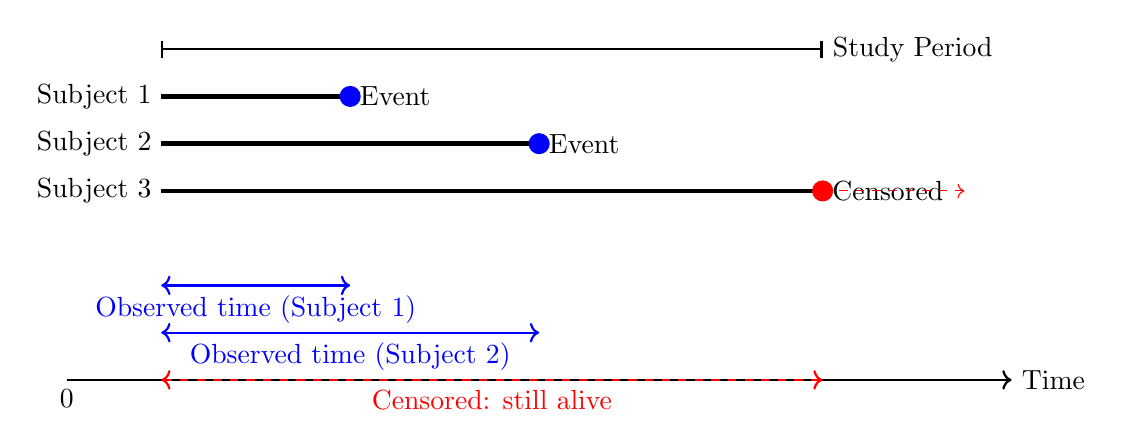
\begin{tikzpicture}[scale=1.2]
        % Timeline
        \draw[->, thick] (0,0) -- (10,0) node[right] {Time};
        \draw (0,0) node[below] {0};

        % Study period
        \draw[|-|, thick] (1,3.5) -- (8,3.5) node[right] {Study Period};

        % Subject 1: Experiences event
        \draw[ultra thick, -] (1,3) -- (3,3);
        \filldraw[blue] (3,3) circle (3pt);
        \node[left] at (1,3) {Subject 1};
        \node[right] at (3,3) {Event};

        % Subject 2: Experiences event
        \draw[ultra thick, -] (1,2.5) -- (5,2.5);
        \filldraw[blue] (5,2.5) circle (3pt);
        \node[left] at (1,2.5) {Subject 2};
        \node[right] at (5,2.5) {Event};

        % Subject 3: Right censored
        \draw[ultra thick, -] (1,2) -- (8,2);
        \filldraw[red] (8,2) circle (3pt);
        \node[left] at (1,2) {Subject 3};
        \node[right] at (8,2) {Censored};
        \draw[red, dashed, ->] (8,2) -- (9.5,2);

        % Observation periods
        \draw[<->, thick, blue] (1,1) -- (3,1) node[midway, below] {Observed time (Subject 1)};
        \draw[<->, thick, blue] (1,0.5) -- (5,0.5) node[midway, below] {Observed time (Subject 2)};
        \draw[<->, thick, red, dashed] (1,0) -- (8,0) node[midway, below] {Censored: still alive};
    \end{tikzpicture}
    \caption{Illustration of right censoring in a clinical study. Subjects 1 and 2 experience the event of interest, while Subject 3 is right-censored at the end of the study period. We know Subject 3 survived at least until time 8, but we don't know their exact event time.}
    \label{fig:right-censoring}
\end{figure}

\subsubsection{Left Censoring}

Left censoring occurs when the event of interest happens before the first observation time, but we don't know exactly when it occurred.

\begin{examplebox}[title=Examples of Left Censoring]
\begin{itemize}
    \item A patient already has the disease when first examined, but we don't know when it developed
    \item Environmental contamination detected at the start of monitoring, but we don't know when it began
    \item A customer had already canceled their subscription before the study began
    \item A component is discovered to be already failed at the first inspection
\end{itemize}

In these cases, we only know that the event occurred \textit{sometime before} the first observation.
\end{examplebox}

Figure \ref{fig:left-censoring} shows left censoring in a disease monitoring study. Subject 1 is found to have the disease at the study entry, representing left censoring.

\begin{figure}[htbp]
    \centering
    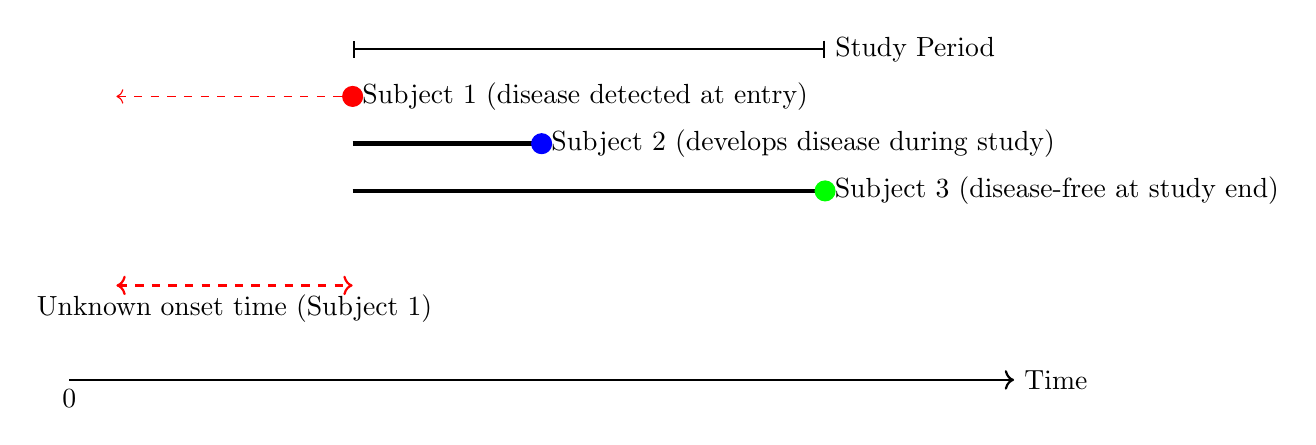
\begin{tikzpicture}[scale=1.2]
        % Timeline
        \draw[->, thick] (0,0) -- (10,0) node[right] {Time};
        \draw (0,0) node[below] {0};

        % Study period
        \draw[|-|, thick] (3,3.5) -- (8,3.5) node[right] {Study Period};

        % Subject 1: Left censored
        \filldraw[red] (3,3) circle (3pt);
        \draw[red, dashed, <-] (0.5,3) -- (3,3);
        \node[right] at (3,3) {Subject 1 (disease detected at entry)};

        % Subject 2: Experiences event
        \draw[ultra thick, -] (3,2.5) -- (5,2.5);
        \filldraw[blue] (5,2.5) circle (3pt);
        \node[right] at (5,2.5) {Subject 2 (develops disease during study)};

        % Subject 3: Right censored
        \draw[ultra thick, -] (3,2) -- (8,2);
        \filldraw[green] (8,2) circle (3pt);
        \node[right] at (8,2) {Subject 3 (disease-free at study end)};

        % Observation arrows
        \draw[<->, thick, red, dashed] (0.5,1) -- (3,1);
        \node[below] at (1.75,1) {Unknown onset time (Subject 1)};
    \end{tikzpicture}
    \caption{Illustration of left censoring. Subject 1 already has the disease when entering the study, so we only know the disease onset occurred sometime before the study entry point.}
    \label{fig:left-censoring}
\end{figure}

\subsubsection{Interval Censoring}

Interval censoring occurs when we know the event occurred within a specific time interval, but not the exact time.

\begin{examplebox}[title=Examples of Interval Censoring]
\begin{itemize}
    \item A tumor is detected during a regular screening visit, but was not present at the previous visit
    \item Infection is detected during a follow-up visit, but was not present at the previous visit
    \item A machine is found to be malfunctioning during a scheduled inspection, but was working at the last inspection
    \item A crack in a structure is discovered during routine examination, but was not present at the previous examination
\end{itemize}

We know the event occurred within the interval between observations, but not the exact time.
\end{examplebox}

Figure \ref{fig:interval-censoring} illustrates interval censoring in a periodic screening context. The condition is detected at Visit 3, but was not present at Visit 2, so the exact onset time is interval-censored between these visits.

\begin{figure}[htbp]
    \centering
    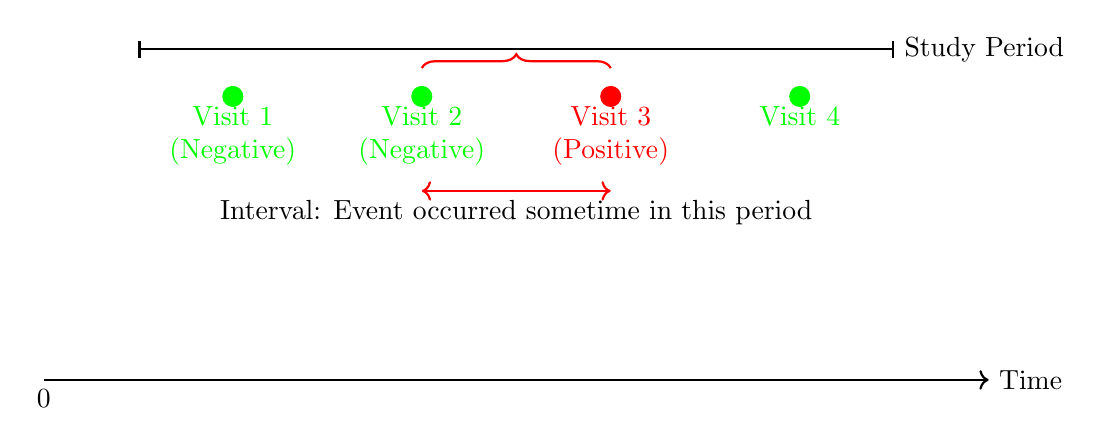
\begin{tikzpicture}[scale=1.2]
        % Timeline
        \draw[->, thick] (0,0) -- (10,0) node[right] {Time};
        \draw (0,0) node[below] {0};

        % Study period
        \draw[|-|, thick] (1,3.5) -- (9,3.5) node[right] {Study Period};

        % Checkup times
        \filldraw[green] (2,3) circle (3pt) node[below, align=center] {Visit 1\\(Negative)};
        \filldraw[green] (4,3) circle (3pt) node[below, align=center] {Visit 2\\(Negative)};
        \filldraw[red] (6,3) circle (3pt) node[below, align=center] {Visit 3\\(Positive)};
        \filldraw[green] (8,3) circle (3pt) node[below] {Visit 4};

        % Interval censoring
        \draw[<->, thick, red] (4,2) -- (6,2);
        \node[below] at (5,2) {Interval: Event occurred sometime in this period};

        % Highlight interval
        \draw[red, thick, decorate, decoration={brace, amplitude=5pt}] (4,3.3) -- (6,3.3);
    \end{tikzpicture}
    \caption{Illustration of interval censoring. The condition is negative at Visit 2 but positive at Visit 3, so we know the onset occurred within this time interval, but not the exact time.}
    \label{fig:interval-censoring}
\end{figure}

\subsection{Time-Varying Effects and Covariates}

In survival analysis, the relationship between predictors and outcomes can change over time:

\begin{itemize}
    \item \textbf{Time-varying effects:} The impact of a covariate on survival may change over time. For example, a treatment might be most effective in the short term but diminish in effectiveness over time.

    \item \textbf{Time-varying covariates:} The values of predictors may change over the course of observation. For instance, a patient's biomarker levels or medication dosages might change throughout a study.
\end{itemize}

\subsection{Multiple Outcomes and Competing Risks}

In many real-world scenarios, subjects may experience different types of events:

\begin{itemize}
    \item \textbf{Competing risks:} Multiple possible event types where the occurrence of one event precludes the observation of others. For example, patients might die from cancer, heart disease, or other causes, but once one cause of death occurs, the others cannot be observed.

    \item \textbf{Recurrent events:} The same event can occur multiple times for a subject, such as hospital readmissions or equipment failures.

    \item \textbf{Multi-state processes:} Subjects can transition through various states over time, like different stages of disease progression.
\end{itemize}

\section{Core Questions in Survival Analysis}

Survival analysis addresses several fundamental questions:

\subsection{Survival Probability Estimation}

What is the probability that a subject will survive (not experience the event) beyond a specific time point? This is typically represented by the \textit{survival function}, denoted as $S(t)$, which gives the probability of surviving beyond time $t$.

\begin{equationbox}[title=Survival Function]
\begin{equation}
S(t) = P(T > t)
\end{equation}

where $T$ is the time-to-event random variable. The survival function has the following properties:
\begin{itemize}
    \item $S(0) = 1$ (all subjects are event-free at the start)
    \item $\lim_{t \to \infty} S(t) = 0$ (eventually all subjects experience the event)
    \item $S(t)$ is monotonically decreasing (survival probability cannot increase with time)
\end{itemize}
\end{equationbox}

Figure \ref{fig:survival-function} shows a typical survival curve, which illustrates how the probability of surviving beyond time $t$ decreases over time.

\begin{figure}[htbp]
    \centering
    \begin{tikzpicture}
        \begin{axis}[
            width=0.8\textwidth,
            height=6cm,
            xlabel={Time},
            ylabel={$S(t)$},
            axis lines=left,
            xmin=0, xmax=10,
            ymin=0, ymax=1.05,
            domain=0:10,
            samples=100
        ]
            % Example survival function
            \addplot[blue, thick] {exp(-0.2*x)};

            % Annotation for specific S(t) value
            \addplot[gray, dashed, samples=2] coordinates {(3,0) (3,0.55)};
            \draw[<->] (axis cs:3.2,0) -- (axis cs:3.2,0.55) node[midway, right] {$S(3) = 0.55$};

            % Median survival
            \addplot[gray, dashed, samples=2] coordinates {(0,0.5) (10,0.5)};
            \addplot[gray, dashed, samples=2] coordinates {(3.47,0) (3.47,0.5)};
            \node[below] at (axis cs:3.47,0) {Median survival};
        \end{axis}
    \end{tikzpicture}
    \caption{A typical survival function showing the probability of surviving beyond time $t$. The dashed lines indicate how to find the median survival time (where $S(t) = 0.5$).}
    \label{fig:survival-function}
\end{figure}

\subsection{Risk Assessment: Hazard Function}

What is the instantaneous risk of experiencing the event at a specific time, given survival up to that time? This is represented by the \textit{hazard function}, denoted as $h(t)$.

\begin{equationbox}[title=Hazard Function]
\begin{equation}
h(t) = \lim_{\Delta t \to 0} \frac{P(t \leq T < t + \Delta t | T \geq t)}{\Delta t}
\end{equation}

The hazard function represents the instantaneous rate of event occurrence at time $t$, conditional on having survived until time $t$.
\end{equationbox}

Unlike the survival function, the hazard function can take many shapes, as illustrated in Figure \ref{fig:hazard-patterns}.

\begin{figure}[htbp]
    \centering
    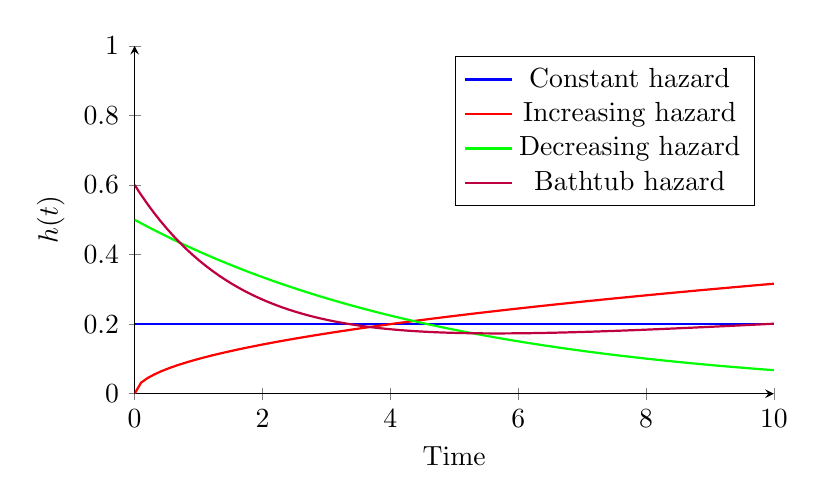
\begin{tikzpicture}
        \begin{axis}[
            width=0.8\textwidth,
            height=6cm,
            xlabel={Time},
            ylabel={$h(t)$},
            axis lines=left,
            xmin=0, xmax=10,
            ymin=0, ymax=1,
            domain=0:10,
            samples=100,
            legend pos=north east
        ]
            % Constant hazard (Exponential distribution)
            \addplot[blue, thick] {0.2};
            \addlegendentry{Constant hazard};

            % Increasing hazard (Weibull with shape > 1)
            \addplot[red, thick] {0.1*x^0.5};
            \addlegendentry{Increasing hazard};

            % Decreasing hazard (Weibull with shape < 1)
            \addplot[green, thick] {0.5*exp(-0.2*x)};
            \addlegendentry{Decreasing hazard};

            % Bathtub hazard (common in reliability)
            \addplot[purple, thick] {0.5*exp(-0.6*x) + 0.1 + 0.01*x};
            \addlegendentry{Bathtub hazard};
        \end{axis}
    \end{tikzpicture}
    \caption{Different patterns of hazard functions. The constant hazard corresponds to the exponential distribution, increasing hazard might indicate aging or wear, decreasing hazard can represent early failures, and the bathtub pattern is common in reliability engineering.}
    \label{fig:hazard-patterns}
\end{figure}

\subsection{Covariate Effects}

How do various factors (covariates) affect survival probabilities and hazard rates? This is typically addressed through regression models that relate covariates to the hazard function or survival function.

\begin{equationbox}[title=Cox Proportional Hazards Model]
\begin{equation}
h(t|\mathbf{X}) = h_0(t) \exp(\boldsymbol{\beta}^T \mathbf{X})
\end{equation}

where $h_0(t)$ is the baseline hazard function, $\mathbf{X}$ is the vector of covariates, and $\boldsymbol{\beta}$ represents the coefficients indicating how each covariate affects the hazard ratio.
\end{equationbox}

\subsection{Group Comparisons}

Are there differences in survival experiences between groups? This is often assessed using non-parametric tests like the log-rank test or through regression modeling.

\subsection{Advanced Questions}

As the field progresses, particularly with the incorporation of machine learning techniques, additional questions are being addressed:

\begin{itemize}
    \item How to model complex, non-linear relationships between covariates and outcomes?
    \item How to incorporate unstructured data (images, text, etc.) into survival models?
    \item How to handle competing risks and multi-state processes efficiently?
    \item How to provide uncertainty quantification for survival predictions?
    \item How to use survival predictions to guide personalized treatment decisions?
\end{itemize}

\section{Traditional Approaches to Survival Analysis}

Survival analysis has traditionally been approached through three main categories of methods: non-parametric, semi-parametric, and fully parametric. Each has its strengths and limitations.

\subsection{Non-Parametric Methods}

Non-parametric methods make no assumptions about the underlying distribution of survival times. They are useful for exploratory analysis and for comparing survival experiences between groups.

\subsubsection{Kaplan-Meier Estimator}

The Kaplan-Meier estimator is the most widely used non-parametric method for estimating the survival function from censored data.

\begin{equationbox}[title=Kaplan-Meier Estimator]
\begin{equation}
\hat{S}(t) = \prod_{t_i \leq t} \left(1 - \frac{d_i}{n_i}\right)
\end{equation}

where:
\begin{itemize}
    \item $t_i$ are the distinct event times observed in the data
    \item $d_i$ is the number of events at time $t_i$
    \item $n_i$ is the number of subjects at risk just before time $t_i$
\end{itemize}
\end{equationbox}

The Kaplan-Meier estimator produces a step function that decreases at each event time, as shown in Figure \ref{fig:kaplan-meier}.

\begin{figure}[htbp]
    \centering
    \begin{tikzpicture}
        \begin{axis}[
            width=0.8\textwidth,
            height=6cm,
            xlabel={Time},
            ylabel={$\hat{S}(t)$},
            axis lines=left,
            ymin=0, ymax=1.05,
            xmin=0, xmax=10,
            xtick={0,2,...,10},
            ytick={0,0.2,...,1},
            domain=0:10,
            samples=100
        ]
            % Step function
            \addplot[blue, thick, const plot, jump mark left] coordinates {
                (0,1) (1,1) (1,0.9)
                (2,0.9) (2,0.8) (3,0.8)
                (3,0.7) (4,0.7) (4,0.6)
                (5,0.6) (5,0.5) (6,0.5)
                (6,0.4) (7,0.4) (7,0.3)
                (8,0.3) (8,0.2) (9,0.2)
                (9,0.1) (10,0.1)
            };

            % Censored points (open circles)
            \addplot[
                only marks,
                mark=o,
                mark options={fill=white, draw=black},
                mark size=2.5pt
            ] coordinates {
                (1.5,0.9)
                (3.5,0.7)
                (6.5,0.4)
                (9.5,0.1)
            };

            % Event markers (filled circles)
            \addplot[
                only marks,
                mark=*,
                color=blue,
                mark size=2pt
            ] coordinates {
                (1,0.9)
                (2,0.8)
                (3,0.7)
                (4,0.6)
                (5,0.5)
                (6,0.4)
                (7,0.3)
                (8,0.2)
                (9,0.1)
            };

            % Median survival
            \addplot[gray, dashed, samples=2] coordinates {(0,0.5) (10,0.5)};
            \addplot[gray, dashed, samples=2] coordinates {(5,0) (5,0.5)};
        \end{axis}
    \end{tikzpicture}
    \caption{Kaplan-Meier survival curve. The step function drops at each event time, and censored observations are shown as open circles. The median survival time is 5 (where the curve crosses the 0.5 probability line).}
    \label{fig:kaplan-meier}
\end{figure}

\subsubsection{Log-Rank Test}

The Log-Rank test is a non-parametric statistical test used to compare survival distributions between two or more groups.

\begin{equationbox}[title=Log-Rank Test Statistic]
\begin{equation}
\chi^2 = \frac{(O_1 - E_1)^2}{E_1} + \frac{(O_2 - E_2)^2}{E_2} + \cdots + \frac{(O_G - E_G)^2}{E_G}
\end{equation}

where:
\begin{itemize}
    \item $O_g$ is the observed number of events in group $g$
    \item $E_g$ is the expected number of events in group $g$ under the null hypothesis
    \item $G$ is the number of groups
\end{itemize}
The test statistic follows a chi-square distribution with $(G-1)$ degrees of freedom under the null hypothesis of no difference between groups.
\end{equationbox}

\subsection{Semi-Parametric Methods}

Semi-parametric methods make some assumptions about the relationship between covariates and hazard, but leave the baseline hazard function unspecified.

\subsubsection{Cox Proportional Hazards Model}

The Cox proportional hazards model is the most widely used regression model in survival analysis. It assumes that the effect of covariates is to multiply the hazard by a constant factor, but makes no assumptions about the shape of the baseline hazard.

\begin{equationbox}[title=Cox Proportional Hazards Model]
\begin{equation}
h(t|\mathbf{X}) = h_0(t) \exp(\boldsymbol{\beta}^T \mathbf{X})
\end{equation}

where:
\begin{itemize}
    \item $h_0(t)$ is the baseline hazard function (left unspecified)
    \item $\mathbf{X}$ is the vector of covariates
    \item $\boldsymbol{\beta}$ is the vector of regression coefficients
\end{itemize}

The key assumption is that the hazard ratio between any two individuals is constant over time (proportional hazards assumption).
\end{equationbox}

The Cox model can be fit using partial likelihood, which allows estimation of $\boldsymbol{\beta}$ without having to specify $h_0(t)$. This makes it very flexible and robust.

\begin{figure}[htbp]
    \centering
    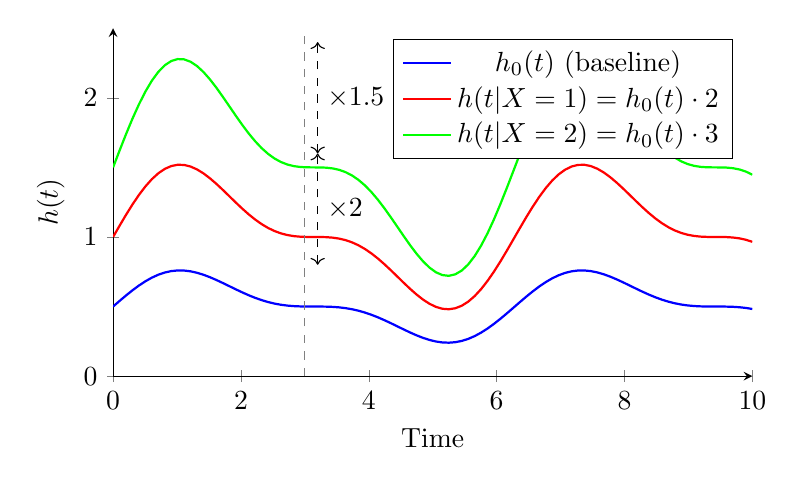
\begin{tikzpicture}
        \begin{axis}[
            width=0.8\textwidth,
            height=6cm,
            xlabel={Time},
            ylabel={$h(t)$},
            axis lines=left,
            ymin=0, ymax=2.5,
            xmin=0, xmax=10,
            domain=0:10,
            samples=100,
            legend pos=north east
        ]
            % Baseline hazard
            \addplot[blue, thick] {0.5 + 0.2*sin(deg(x)) + 0.1*sin(deg(2*x))};
            \addlegendentry{$h_0(t)$ (baseline)};

            % Proportional hazard for X=1
            \addplot[red, thick] {2*(0.5 + 0.2*sin(deg(x)) + 0.1*sin(deg(2*x)))};
            \addlegendentry{$h(t|X=1) = h_0(t) \cdot 2$};

            % Proportional hazard for X=2
            \addplot[green, thick] {3*(0.5 + 0.2*sin(deg(x)) + 0.1*sin(deg(2*x)))};
            \addlegendentry{$h(t|X=2) = h_0(t) \cdot 3$};

            % Vertical reference line
            \addplot[gray, dashed, samples=2] coordinates {(3,0) (3,2.5)};

            % Proportional hazards illustration
            \draw[<->, dashed] (axis cs:3.2,0.8) -- (axis cs:3.2,1.6) node[midway, right] {$\times 2$};
            \draw[<->, dashed] (axis cs:3.2,1.6) -- (axis cs:3.2,2.4) node[midway, right] {$\times 1.5$};
        \end{axis}
    \end{tikzpicture}
    \caption{Illustration of the proportional hazards assumption in the Cox model. The hazard ratios between different covariate values remain constant over time, regardless of the shape of the baseline hazard.}
    \label{fig:proportional-hazards}
\end{figure}

\subsubsection{Extensions of the Cox Model}

Several extensions of the Cox model have been developed to address specific limitations:

\begin{itemize}
    \item \textbf{Stratified Cox model:} Allows for different baseline hazards across strata while maintaining the same covariate effects.

    \item \textbf{Time-dependent Cox model:} Allows for time-varying covariates and time-varying effects through terms like $X(t)$ and $\beta(t)$.

    \item \textbf{Frailty models:} Incorporate random effects to account for unobserved heterogeneity and clustering in the data.

    \item \textbf{Competing risks extensions:} Adaptations for handling competing events, such as cause-specific Cox models and Fine-Gray models.
\end{itemize}

\subsection{Fully Parametric Methods}

Parametric methods specify a full probability distribution for the survival times. These methods are more efficient when the distributional assumptions are correct and allow for direct modeling of the survival time rather than just the hazard.

\subsubsection{Common Parametric Distributions}

Several probability distributions are commonly used in parametric survival analysis:

\paragraph{Exponential Distribution}
The exponential distribution assumes a constant hazard rate, which corresponds to a memoryless process.

\begin{equationbox}[title=Exponential Distribution]
\begin{align}
h(t) &= \lambda\\
S(t) &= e^{-\lambda t}\\
f(t) &= \lambda e^{-\lambda t}
\end{align}

where $\lambda > 0$ is the rate parameter.
\end{equationbox}

\paragraph{Weibull Distribution}
The Weibull distribution allows for both increasing and decreasing hazard rates, depending on the shape parameter.

\begin{equationbox}[title=Weibull Distribution]
\begin{align}
h(t) &= \alpha \lambda (\lambda t)^{\alpha-1}\\
S(t) &= e^{-(\lambda t)^\alpha}\\
f(t) &= \alpha \lambda (\lambda t)^{\alpha-1} e^{-(\lambda t)^\alpha}
\end{align}

where $\alpha > 0$ is the shape parameter and $\lambda > 0$ is the scale parameter.
\begin{itemize}
    \item If $\alpha = 1$, the Weibull reduces to the exponential distribution
    \item If $\alpha > 1$, the hazard increases with time
    \item If $\alpha < 1$, the hazard decreases with time
\end{itemize}
\end{equationbox}

\paragraph{Log-normal and Log-logistic Distributions}
These distributions can model non-monotonic hazard rates, where the hazard first increases and then decreases over time.

\paragraph{Generalized Gamma Distribution}
A flexible three-parameter family that includes many other distributions as special cases.

\begin{figure}[htbp]
    \centering
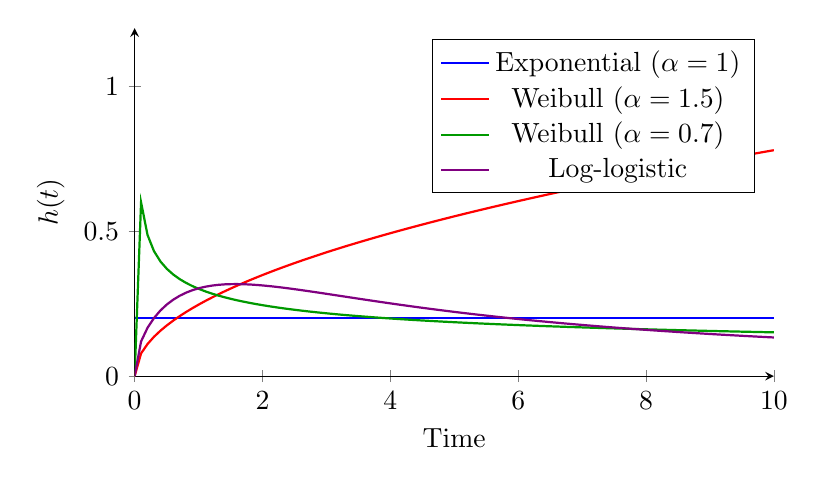
\begin{tikzpicture}
    \begin{axis}[
        width=0.8\textwidth,
        height=6cm,
        xlabel={Time},
        ylabel={$h(t)$},
        axis lines=left,
        ymin=0, ymax=1.2,
        xmin=0, xmax=10,
        domain=0:10,
        samples=100,
        legend pos=north east
    ]
        % Exponential hazard (constant)
        \addplot[blue, thick] {0.2};
        \addlegendentry{Exponential ($\alpha=1$)};

        % Weibull increasing
        \addplot[red, thick] {0.45 * pow(0.3*x, 0.5)};
        \addlegendentry{Weibull ($\alpha=1.5$)};

        % Weibull decreasing
        \addplot[green!60!black, thick] {0.21 * pow(0.3*x, -0.3)};
        \addlegendentry{Weibull ($\alpha=0.7$)};

        % Log-logistic (non-monotonic)
        \addplot[violet, thick] {0.6 * pow(0.4*x, 0.5) / (1 + pow(0.4*x, 1.5))};
        \addlegendentry{Log-logistic};
    \end{axis}
\end{tikzpicture}
    \caption{Hazard functions for different parametric survival distributions. Note how the shape parameter in the Weibull distribution controls whether the hazard increases or decreases with time, while the log-logistic allows for a non-monotonic hazard.}
    \label{fig:parametric-hazards}
\end{figure}

\subsubsection{Parametric Regression Models}

Parametric regression models relate covariates to the parameters of these distributions. For example, in a Weibull regression model:

\begin{equationbox}[title=Parametric Regression Model]
\begin{equation}
h(t|\mathbf{X}) = \alpha \lambda(\mathbf{X}) (\lambda(\mathbf{X}) t)^{\alpha-1}
\end{equation}

where $\lambda(\mathbf{X}) = \lambda_0 \exp(\boldsymbol{\beta}^T \mathbf{X})$, allowing covariates to affect the scale parameter.
\end{equationbox}

\section{Limitations of Traditional Methods}

Despite their utility, traditional survival analysis methods face several important limitations that have motivated the development of more advanced approaches.

\subsection{Modeling Constraints}

\subsubsection{Linear Relationship Assumptions}

Traditional methods typically assume linear relationships between covariates and the log hazard or log survival time. This can be limiting when:

\begin{itemize}
    \item The true relationships are non-linear
    \item Complex interactions exist between covariates
    \item The effect of a predictor varies substantially across its range
\end{itemize}

While transformations and interaction terms can address some of these issues, they require manual specification and prior knowledge of the functional form.

\subsubsection{Restrictive Functional Forms}

Parametric models are constrained by the chosen probability distribution:

\begin{itemize}
    \item Limited flexibility in modeling complex hazard patterns
    \item Distribution selection can significantly affect results
    \item Multimodal hazard functions are difficult to capture
\end{itemize}

\subsection{High-Dimensional Data Challenges}

Traditional survival methods were not designed for modern high-dimensional data:

\begin{itemize}
    \item Poor performance with large numbers of features
    \item Inability to directly handle unstructured data (images, text, signals)
    \item Need for extensive feature engineering
    \item Difficulty in capturing complex interactions automatically
    \item Inefficient with sparse or noisy features
\end{itemize}

\subsection{Time-Varying Challenges}

Handling time-varying aspects presents significant challenges:

\begin{itemize}
    \item Complex implementation for time-varying covariates
    \item Special techniques needed for non-proportional hazards
    \item Limited ability to capture temporal patterns automatically
    \item Difficulty handling irregular time series
\end{itemize}

\section{Modern Deep Learning Approaches}

To address these limitations, researchers have developed a range of deep learning approaches for survival analysis, which fall into several categories.

\subsection{Neural Cox Extensions}

These methods maintain the semi-parametric nature of the Cox model but replace the linear predictor with neural networks.

\begin{equationbox}[title=Neural Cox Models]
\begin{equation}
h(t|\mathbf{X}) = h_0(t) \exp(f_{\text{NN}}(\mathbf{X}))
\end{equation}

where $f_{\text{NN}}(\mathbf{X})$ is a neural network function of the input features.
\end{equationbox}

Examples include:
\begin{itemize}
    \item DeepSurv: Uses feedforward neural networks with the partial likelihood
    \item Cox-Time: Extends to time-varying effects through neural networks
\end{itemize}

\subsection{Discrete-Time Neural Survival Models}

These approaches discretize time into intervals and predict the conditional probability of an event in each interval, often implementing this as a sequence prediction problem.

\begin{equationbox}[title=Discrete-Time Survival Models]
\begin{equation}
P(t_k \leq T < t_{k+1} | T \geq t_k, \mathbf{X}) = f_{\text{NN},k}(\mathbf{X})
\end{equation}

where $f_{\text{NN},k}(\mathbf{X})$ is the output of a neural network for the $k$-th time interval.
\end{equationbox}

Examples include:
\begin{itemize}
    \item Nnet-survival: Uses multi-task logistic regression for each discrete time interval
    \item DeepHit: Predicts the probability mass function across discretized time intervals
\end{itemize}

\subsection{Deep Parametric Survival Models}

These models use neural networks to parameterize probability distributions, allowing for flexible modeling of complex survival patterns.

\begin{equationbox}[title=Deep Parametric Survival Models]
\begin{equation}
S(t|\mathbf{X}) = S(t|\boldsymbol{\theta}_{\text{NN}}(\mathbf{X}))
\end{equation}

where $\boldsymbol{\theta}_{\text{NN}}(\mathbf{X})$ are the distribution parameters learned by neural networks.
\end{equationbox}

Examples include:
\begin{itemize}
    \item Deep Survival Machines (DSM): Uses a mixture of parametric distributions
    \item Deep Weibull: Parameterizes Weibull distributions with neural networks
\end{itemize}

\subsection{Representation-Focused Models}

These approaches focus on learning powerful representations from complex input data:

\begin{itemize}
    \item Survival transformers: Use attention mechanisms for feature interactions
    \item Recurrent neural networks: For temporal data and time-varying covariates
    \item Graph neural networks: For structured relationship data
    \item Multi-task survival learning: For joint prediction of related outcomes
\end{itemize}

\section{Advantages of Deep Learning for Survival Analysis}

Deep learning approaches offer several important advantages for survival analysis:

\subsection{Feature Learning}

Neural networks can automatically extract relevant features from raw data:

\begin{itemize}
    \item Direct learning from unstructured data (images, text, signals)
    \item Transfer learning from pre-trained representations
    \item Reduced need for manual feature engineering
    \item Ability to handle high-dimensional inputs efficiently
\end{itemize}

\subsection{Flexible Relationship Modeling}

Deep learning models can capture complex relationships:

\begin{itemize}
    \item Non-linear relationships between covariates and hazards
    \item Automatic interaction detection
    \item Handling of high-dimensional feature spaces
    \item Implicit regularization through network architecture
\end{itemize}

\subsection{Beyond Proportional Hazards}

Neural networks can model more complex hazard patterns:

\begin{itemize}
    \item Non-proportional hazards without explicit specification
    \item Time-varying effects handled naturally
    \item Complex temporal patterns learned from data
    \item Multi-modal hazard distributions
\end{itemize}

\subsection{Multi-Event Modeling}

Deep learning facilitates joint prediction of multiple outcomes:

\begin{itemize}
    \item Simultaneous prediction of multiple event types
    \item Capturing dependencies between different events
    \item Flexible competing risks modeling
    \item Information sharing across related outcomes
\end{itemize}

\section{Course Roadmap}

This book presents a comprehensive learning path from traditional survival analysis to advanced deep learning approaches, organized as follows:

\subsection{Foundations (Chapters 1-3)}

\begin{itemize}
    \item Introduction to survival analysis concepts
    \item Statistical foundations and likelihood principles
    \item Traditional survival models and their limitations
\end{itemize}

\subsection{Data Representation (Chapter 4)}

\begin{itemize}
    \item Handling survival data in deep learning
    \item Embedding techniques for categorical and continuous features
    \item Representation learning for survival analysis
\end{itemize}

\subsection{Deep Survival Models (Chapters 5-7)}

\begin{itemize}
    \item Deep Survival Machines (DSM)
    \item Multi-Event Neural Survival Analysis (MENSA)
    \item Loss functions for survival prediction
\end{itemize}

\subsection{Advanced Topics (Chapters 8-9)}

\begin{itemize}
    \item Numerical stability in survival models
    \item Expert knowledge integration
    \item Applications and case studies
\end{itemize}

\begin{figure}[htbp]
    \centering
    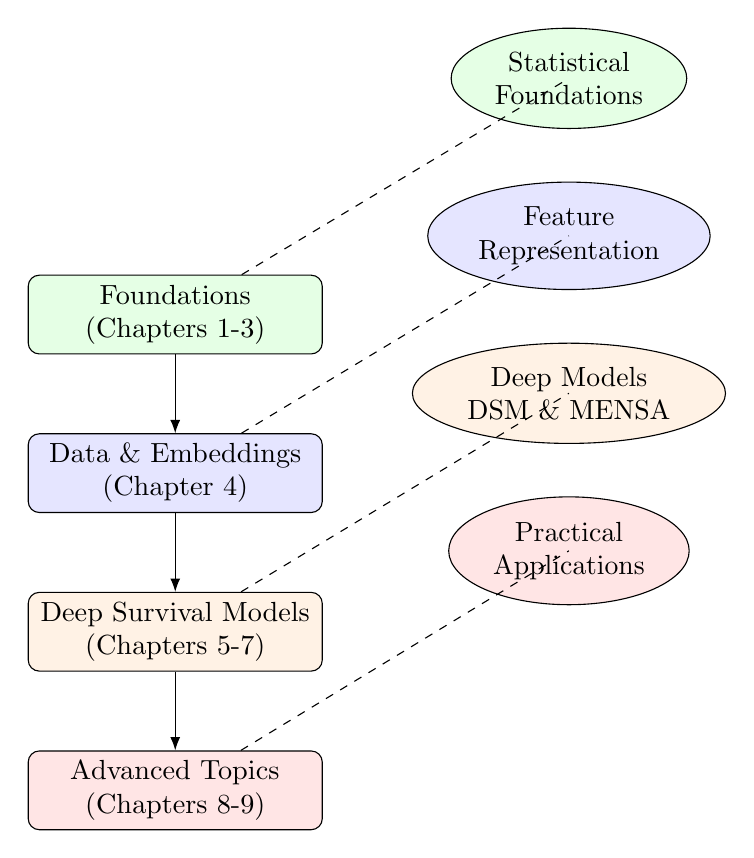
\begin{tikzpicture}[
        node distance=1cm,
        box/.style={rectangle, rounded corners, draw, fill=blue!10, text width=3.5cm, minimum height=1cm, align=center}
    ]
        % Basic learning path
        \node[box, fill=green!10] (foundations) {Foundations\\(Chapters 1-3)};
        \node[box, fill=blue!10, below=of foundations] (data) {Data \& Embeddings\\(Chapter 4)};
        \node[box, fill=orange!10, below=of data] (models) {Deep Survival Models\\(Chapters 5-7)};
        \node[box, fill=red!10, below=of models] (advanced) {Advanced Topics\\(Chapters 8-9)};

        % Connecting arrows
        \draw[-Latex] (foundations) -- (data);
        \draw[-Latex] (data) -- (models);
        \draw[-Latex] (models) -- (advanced);

        % Content highlights on the right
        \node[draw, ellipse, fill=green!10, align=center] at (5,3) {Statistical\\Foundations};
        \node[draw, ellipse, fill=blue!10, align=center] at (5,1) {Feature\\Representation};
        \node[draw, ellipse, fill=orange!10, align=center] at (5,-1) {Deep Models\\DSM \& MENSA};
        \node[draw, ellipse, fill=red!10, align=center] at (5,-3) {Practical\\Applications};

        % Connect highlights to path
        \draw[dashed] (foundations) -- (5,3);
        \draw[dashed] (data) -- (5,1);
        \draw[dashed] (models) -- (5,-1);
        \draw[dashed] (advanced) -- (5,-3);
    \end{tikzpicture}
    \caption{Course roadmap showing the progression from foundational concepts to advanced topics in deep learning for survival analysis.}
    \label{fig:course-roadmap}
\end{figure}

Each chapter builds on the knowledge from previous chapters, providing a structured learning path from fundamental concepts to cutting-edge research in deep learning for survival analysis.


\chapter{Motivation and Problem Setting}
\label{ch:motivation}
\section{The Need for Time-to-Event Analysis}

Many real-world scenarios require us to understand not just \textit{if} an event will occur, but \textit{when} it might happen. This timing aspect adds complexity to traditional predictive modeling approaches, but also provides valuable information that can lead to better decision-making and outcomes.

\begin{notebox}[title=Time-to-Event Questions Across Domains]
  Time-to-event analysis answers crucial questions across numerous fields:
  \begin{itemize}
  \item \textbf{Healthcare:} When will a patient experience disease progression? How long will a treatment remain effective?
  \item \textbf{Engineering:} How long will a mechanical component function before failure? When should maintenance be scheduled?
  \item \textbf{Business:} When will a customer likely cancel their subscription? When might an employee leave the company?
  \item \textbf{Technology:} When will a system failure occur? What is the expected lifetime of a software feature?
  \end{itemize}
\end{notebox}

Traditional predictive models typically focus on classification (will an event occur?) or regression (how much of something will occur?), but time-to-event analysis introduces a temporal dimension that requires specialized methodologies. Without proper handling of the time component, predictions can be severely biased and lead to incorrect conclusions.

\section{Applications Across Domains}

The need for time-to-event analysis spans virtually every field where timing information is critical for decision-making.

\subsection{Healthcare Applications}

In medicine, understanding the timing of events can directly impact treatment decisions and patient outcomes:

\begin{itemize}
\item \textbf{Patient survival analysis:} Estimating survival time after diagnosis or treatment
\item \textbf{Disease progression:} Predicting time to progression or recurrence
\item \textbf{Treatment efficacy:} Determining duration of treatment effectiveness
\item \textbf{Adverse event timing:} Analyzing when side effects might occur
\item \textbf{Hospital readmission:} Predicting when patients might return after discharge
\item \textbf{Clinical trial analysis:} Comparing time-to-event outcomes between treatment groups
\end{itemize}

Time-to-event analysis in healthcare directly informs treatment planning, resource allocation, and the development of clinical guidelines.

\subsection{Engineering and Reliability Applications}

In engineering contexts, time-to-event analysis helps optimize maintenance schedules, warranty periods, and resource allocation:

\begin{itemize}
\item \textbf{Equipment failure prediction:} Estimating when machinery might fail
\item \textbf{Component lifetime estimation:} Predicting the functional lifespan of parts
\item \textbf{Maintenance optimization:} Scheduling preventive maintenance to minimize downtime
\item \textbf{System reliability assessment:} Evaluating the reliability of complex systems over time
\item \textbf{Warranty period modeling:} Setting appropriate warranty terms based on failure timing
\item \textbf{Quality control:} Analyzing time-to-failure patterns to improve manufacturing
\end{itemize}

These applications help reduce costs, improve safety, and enhance product quality.

\subsection{Business and Economic Applications}

In business contexts, time-to-event analysis provides insights into customer behavior, employee retention, and financial risk:

\begin{itemize}
\item \textbf{Customer churn prediction:} Forecasting when customers might leave
\item \textbf{Subscription lifecycle:} Modeling subscription duration patterns
\item \textbf{Employee retention:} Predicting when employees might leave
\item \textbf{Loan default timing:} Estimating when borrowers might default
\item \textbf{Insurance claim occurrence:} Predicting timing of insurance claims
\item \textbf{Project completion:} Modeling time-to-completion for projects
\end{itemize}

These applications help businesses optimize resource allocation, improve customer retention strategies, and manage financial risk.

\subsection{Other Diverse Applications}

Time-to-event analysis extends to many other fields:

\begin{itemize}
\item \textbf{Social sciences:} Modeling unemployment duration, marriage longevity
\item \textbf{Technology:} Predicting software bug discovery rates, digital content lifespan
\item \textbf{Environmental science:} Analyzing timing of extreme events, species extinction risks
\item \textbf{Academia:} Studying citation timing, research impact evolution
\item \textbf{Public policy:} Evaluating time-dependent effects of policy interventions
\end{itemize}

The ubiquity of time-to-event questions across domains highlights the critical importance of developing robust methodologies for modeling and analyzing such data.

\section{Unique Characteristics of Time-to-Event Data}

Time-to-event data presents several distinct challenges that require specialized analytical approaches. These characteristics make standard regression or classification methods inadequate without careful modification.

\subsection{Incomplete Observations}

Unlike conventional datasets where each observation has a complete set of values, time-to-event data frequently includes incomplete observations—a phenomenon known as censoring. Censoring occurs when the event of interest is not observed for some subjects, but we still have partial information about their event times.

In a clinical study, for example, patients may:
\begin{itemize}
\item Still be alive at the end of the study period
\item Withdraw from the study before experiencing the event
\item Be lost to follow-up for various reasons
\end{itemize}

These incomplete observations contain valuable information that must be properly incorporated into the analysis rather than discarded.

\subsection{Variable Follow-up Durations}

Subject follow-up periods typically vary considerably within a single dataset, with some subjects observed for short periods and others for much longer. This variability creates challenges for standardizing predictions and assessing model performance.

\subsection{Time-Varying Covariates}

Many predictors in time-to-event contexts change over the observation period. For example:
\begin{itemize}
\item A patient's biomarker values may fluctuate during treatment
\item A machine's operational parameters may shift over time
\item A customer's engagement metrics may evolve throughout the relationship
\end{itemize}

These dynamic covariates need special handling to accurately model their effects on the timing of events.

\subsection{Multiple Competing Events}

In many real-world scenarios, subjects may experience various mutually exclusive events:
\begin{itemize}
\item A patient might die from cancer, heart disease, or other causes
\item A mechanical system might fail due to wear, electrical issues, or external damage
\item A customer might churn for different reasons (price, service quality, competitor offers)
\end{itemize}

These competing events require models that can account for multiple possible outcomes and their interdependencies.

\subsection{Informative Observation Patterns}

In time-to-event data, the pattern of observations itself may contain information relevant to the outcome. For example, the frequency of patient visits might correlate with disease severity, or the timing of system inspections might relate to suspected issues. This informative missingness adds another layer of complexity to the analysis.

\section{The Fundamental Challenge: Censoring}

Censoring—the partial observation of event times—represents the most distinctive and challenging aspect of time-to-event data. Censoring occurs when we don't observe the exact time of the event for a subject, but we have some information about when it might have occurred.

A comprehensive discussion of censoring types, mechanisms, and their implications can be found in Chapter \ref{ch:censoring}. Here, we highlight the key challenges that censoring introduces in time-to-event analysis.

\begin{notebox}[title=Key Challenges with Censored Data]
Censoring introduces several unique challenges:
\begin{itemize}
\item Standard statistical methods cannot be directly applied
\item Naive approaches (ignoring censored observations or treating censoring times as event times) lead to biased results
\item Different forms of censoring require different analytical approaches
\item Assumptions about the censoring mechanism are critical for valid inference
\end{itemize}
\end{notebox}

\section{Visualizing Survival Data}

A comprehensive visual representation of survival data helps illustrate the unique challenges of time-to-event analysis. Figure \ref{fig:survival-data-viz} shows a typical survival dataset with varying follow-up times and both observed events and censored observations.

\begin{figure}[htbp]
  \centering
  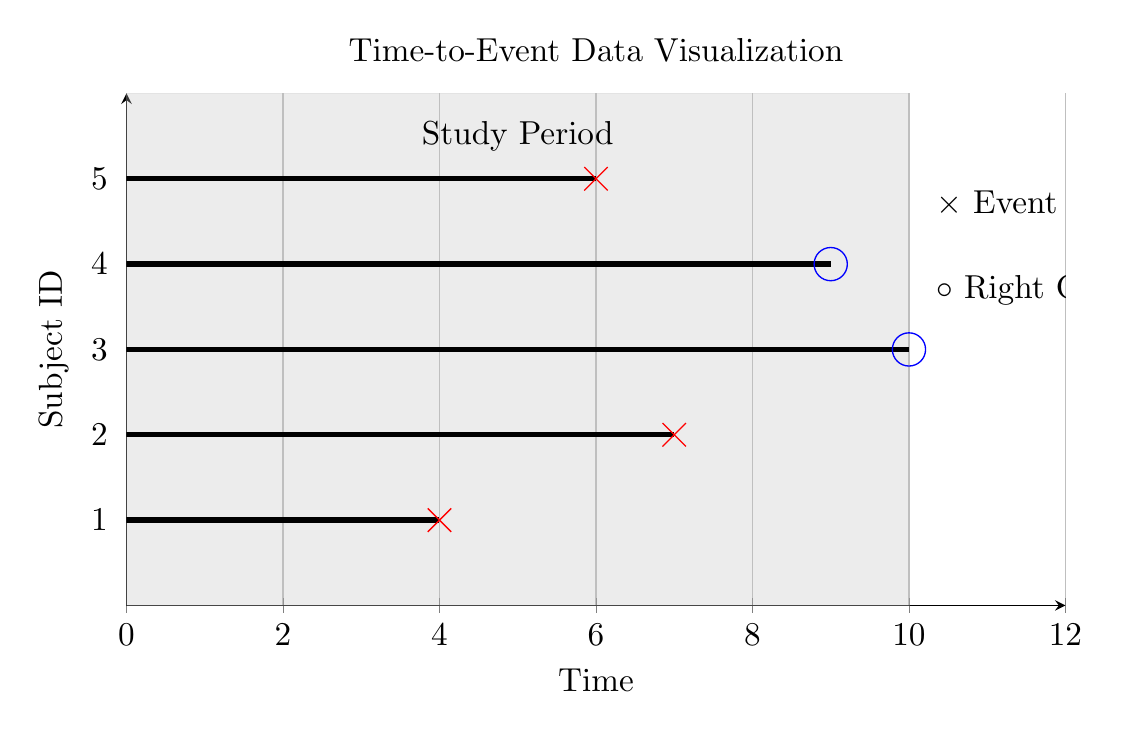
\begin{tikzpicture}[scale=1.2]
    \begin{axis}[
        width=0.95\textwidth,
        height=7cm,
        xlabel={Time},
        ylabel={Subject ID},
        axis lines=left,
        ymin=0,
        ymax=6,
        xmin=0,
        xmax=12,
        ytick={1,2,3,4,5},
        ytick style={draw=none},
        xmajorgrids=true,
        title={Time-to-Event Data Visualization},
      ]
      % Study period
      \addplot[color=lightgray, fill=lightgray, opacity=0.3] coordinates {
        (0,0) (0,6) (10,6) (10,0)
      } \closedcycle;
      \node at (axis cs:5,5.5) {Study Period};

      % Subject follow-up lines
      \addplot[ultra thick, -] coordinates {(0,1) (4,1)};
      \addplot[ultra thick, -] coordinates {(0,2) (7,2)};
      \addplot[ultra thick, -] coordinates {(0,3) (10,3)};
      \addplot[ultra thick, -] coordinates {(0,4) (9,4)};
      \addplot[ultra thick, -] coordinates {(0,5) (6,5)};

      % Events
      \addplot[mark=x, color=red, mark size=5pt] coordinates {(4,1)};
      \addplot[mark=x, color=red, mark size=5pt] coordinates {(7,2)};
      \addplot[mark=o, color=blue, mark size=5pt] coordinates {(10,3)};
      \addplot[mark=o, color=blue, mark size=5pt] coordinates {(9,4)};
      \addplot[mark=x, color=red, mark size=5pt] coordinates {(6,5)};

      % Legend
      \node[anchor=north west] at (axis cs:10.2,5) {$\times$ Event Observed};
      \node[anchor=north west] at (axis cs:10.2,4) {$\circ$ Right Censored};
    \end{axis}
  \end{tikzpicture}
  \caption{Visualization of time-to-event data for five subjects. Each horizontal line represents a subject's follow-up period. Red crosses indicate observed events, while blue circles represent right-censored observations. Note the varying follow-up durations and the mixture of event types.}
  \label{fig:survival-data-viz}
\end{figure}

This visualization highlights several key characteristics of survival data:

\begin{itemize}
\item \textbf{Variable follow-up durations:} Subjects are observed for different periods
\item \textbf{Mixture of observed events and censoring:} Some subjects experience the event during observation, while others are censored
\item \textbf{Administrative censoring:} Some subjects are censored at the study end
\item \textbf{Early withdrawals:} Some subjects exit the study before its conclusion
\end{itemize}

\section{Competing Risks: Another Challenge}

Another significant challenge in time-to-event analysis is the presence of competing risks—multiple possible event types where the occurrence of one event precludes the observation of others. Chapter \ref{ch:censoring} provides a detailed discussion of competing risks, their analysis, and modeling approaches.

Competing risks fundamentally change how we approach survival analysis:

\begin{itemize}
\item \textbf{Event-specific hazards:} Each event type has its own hazard function
\item \textbf{Cumulative incidence functions:} Standard Kaplan-Meier estimates become inappropriate; we need to use cumulative incidence functions that account for competing events
\item \textbf{Interpretation changes:} Risk factors may have different effects on different event types
\item \textbf{Modeling complexity:} Models must account for the interdependence between different event types
\end{itemize}

Ignoring competing risks can lead to substantial biases, particularly the overestimation of event probabilities when using standard survival methods.

\section{Beyond Binary Events: Complex Time-to-Event Scenarios}

Real-world time-to-event scenarios often extend beyond simple binary events (occurred/not occurred) to include more complex patterns:

\subsection{Recurrent Events}

Many events can occur multiple times for the same subject:

\begin{itemize}
\item Hospital readmissions
\item Equipment failures and repairs
\item Episodic disease flares
\item Repeated customer purchases
\end{itemize}

Recurrent event analysis requires specialized methods that can model the correlation between events within the same subject and account for potential changes in risk patterns after each event.

\subsection{Multi-State Processes}

In multi-state processes, subjects can transition through various states over time:

\begin{itemize}
\item Disease progression through different stages
\item Employee transitions between roles
\item Customer journey through different product tiers
\item System transitions between operational states
\end{itemize}

Multi-state models extend survival analysis to handle these complex transition patterns, with each transition potentially having its own risk factors and temporal patterns.

\begin{figure}[htbp]
  \centering
  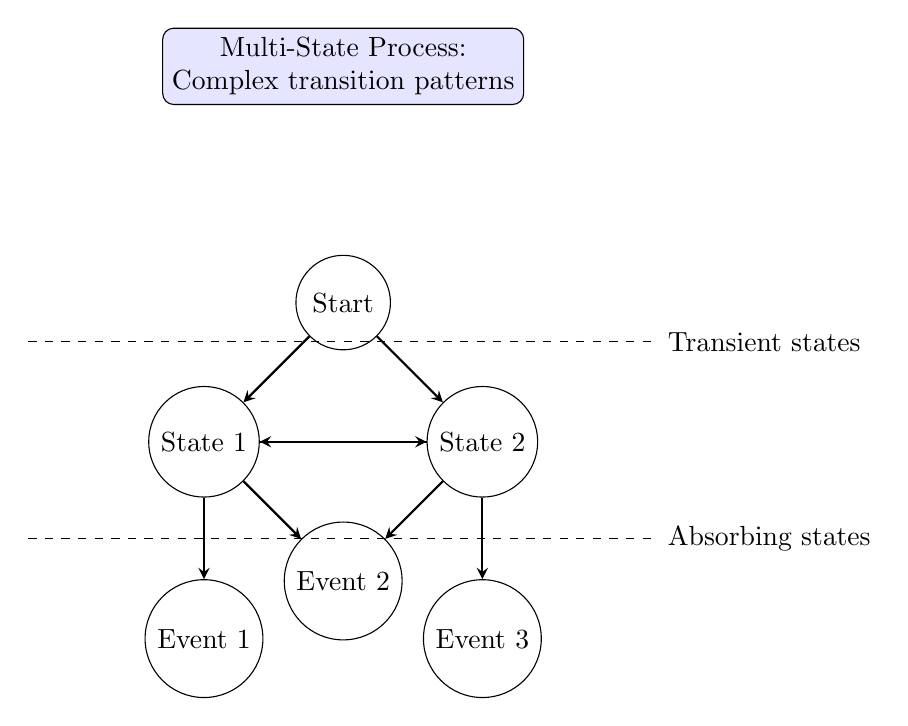
\begin{tikzpicture}[
      node distance=2.5cm,
      state/.style={circle, draw, minimum size=1.2cm},
      arrow/.style={->, >=stealth, thick}
    ]
    % States
    \node[state] (start) {Start};
    \node[state, below left of=start] (state1) {State 1};
    \node[state, below right of=start] (state2) {State 2};
    \node[state, below of=state1] (event1) {Event 1};
    \node[state, below of=state2] (event3) {Event 3};
    \node[state, below right of=state1] (event2) {Event 2};

    % Transitions
    \draw[arrow] (start) -- (state1);
    \draw[arrow] (start) -- (state2);
    \draw[arrow] (state1) -- (state2);
    \draw[arrow] (state2) -- (state1);
    \draw[arrow] (state1) -- (event1);
    \draw[arrow] (state1) -- (event2);
    \draw[arrow] (state2) -- (event2);
    \draw[arrow] (state2) -- (event3);

    % Annotations
    \node[draw, rounded corners, fill=blue!10, align=center] at (0,3) {
      Multi-State Process:\\
      Complex transition patterns
    };
    \draw[dashed] (-4,-0.5) -- (4,-0.5) node[right] {Transient states};
    \draw[dashed] (-4,-3) -- (4,-3) node[right] {Absorbing states};
  \end{tikzpicture}
  \caption{A multi-state process model. Subjects can transition between transient states and eventually reach absorbing states (terminal events). Each transition has its own hazard function that may depend on subject characteristics and history.}
  \label{fig:multi-state}
\end{figure}

\subsection{Joint Longitudinal and Time-to-Event Data}

In many applications, we observe both:
\begin{itemize}
\item Longitudinal measurements of variables over time (e.g., biomarkers, system parameters)
\item Time-to-event outcomes (e.g., failure, disease progression)
\end{itemize}

Joint models for longitudinal and time-to-event data enable:
\begin{itemize}
\item Incorporating time-varying measurements into event predictions
\item Accounting for measurement error in longitudinal data
\item Addressing informative dropout in longitudinal studies
\item Providing dynamic, updated predictions as new measurements arrive
\end{itemize}

\section{Summary}

The unique characteristics of time-to-event data—particularly censoring, variable follow-up durations, competing risks, and complex event patterns—necessitate specialized analytical approaches. Standard regression and classification methods are inadequate without proper adaptation to handle these distinctive features.

The next chapters will explore both traditional and modern approaches to addressing these challenges, beginning with the statistical foundations of survival analysis and progressing to advanced deep learning methods. By understanding these specialized techniques, we can extract meaningful insights from time-to-event data across diverse domains, leading to better predictions, improved decision-making, and ultimately better outcomes.


\chapter{Survival Analysis Foundations}
\label{ch:foundations}
\section{Foundations of Survival Analysis}

Survival analysis comprises a rich collection of statistical methods specifically designed to analyze time-to-event data \parencite{kleinbaum2012}. As introduced in previous chapters, these methods address scenarios where the primary interest is the timing of events rather than just whether they occur \parencite{cox1972}. This chapter provides a comprehensive overview of the mathematical foundations and core concepts that underpin both traditional and modern survival analysis approaches.

\begin{notebox}[title=Chapter Overview]
This chapter covers:
\begin{itemize}
    \item Core mathematical functions in survival analysis and their relationships
    \item Types and properties of hazard functions
    \item Statistical handling of censored observations
    \item Likelihood construction for survival data
    \item Non-parametric estimation approaches
    \item Semi-parametric modeling with Cox proportional hazards
    \item Competing risks methodologies
    \item Limitations of classical methods
\end{itemize}
\end{notebox}

Understanding these foundations is crucial for properly interpreting results and developing innovative approaches to survival analysis, particularly when working with complex real-world datasets and modern machine learning techniques.

\section{Mathematical Framework of Survival Analysis}

Survival analysis is built upon a set of interrelated mathematical functions that provide different perspectives on time-to-event processes. Each function offers unique insights, but they are all mathematically connected, forming a coherent framework for analysis.

\subsection{Core Functions and Their Definitions}

Let $T$ be a non-negative random variable representing the time until an event of interest occurs. The distribution of $T$ can be characterized by several equivalent functions:

\begin{definitionbox}[title=Survival Function]
The \textbf{survival function}, denoted $S(t)$, represents the probability that the event has not occurred by time $t$:
\begin{equation}
    S(t) = P(T > t)
\end{equation}

Key properties:
\begin{itemize}
    \item $S(0) = 1$ (all subjects event-free at the start)
    \item $\lim_{t \to \infty} S(t) = 0$ (eventually all subjects experience the event)
    \item $S(t)$ is monotonically decreasing (risk never decreases with time)
    \item $S(t)$ is right-continuous
\end{itemize}
\end{definitionbox}

The survival function provides a direct measure of the proportion of subjects who remain event-free over time, making it particularly useful for visualization and communicating results to non-specialists.

\begin{definitionbox}[title=Cumulative Distribution Function]
The \textbf{cumulative distribution function (CDF)}, denoted $F(t)$, represents the probability that the event has occurred by time $t$:
\begin{equation}
    F(t) = P(T \leq t) = 1 - S(t)
\end{equation}

Key properties:
\begin{itemize}
    \item $F(0) = 0$ (no events at the start)
    \item $\lim_{t \to \infty} F(t) = 1$ (eventually all subjects experience the event)
    \item $F(t)$ is monotonically increasing
    \item $F(t)$ is right-continuous
\end{itemize}
\end{definitionbox}

While the CDF is the standard representation for random variables in probability theory, survival analysis often focuses on the survival function instead, as it directly captures the concept of "surviving" beyond a specific time point.

\begin{definitionbox}[title=Probability Density Function]
The \textbf{probability density function (PDF)}, denoted $f(t)$, represents the instantaneous rate of event occurrence at exactly time $t$:
\begin{equation}
    f(t) = \frac{d}{dt}F(t) = -\frac{d}{dt}S(t)
\end{equation}

Key properties:
\begin{itemize}
    \item $f(t) \geq 0$ for all $t$
    \item $\int_0^\infty f(t)dt = 1$
    \item $P(t_1 < T \leq t_2) = \int_{t_1}^{t_2} f(t)dt$
\end{itemize}
\end{definitionbox}

The PDF represents the unconditional instantaneous probability of the event occurring at time $t$. This differs from the hazard function, which considers the conditional probability given survival to time $t$.

\begin{definitionbox}[title=Hazard Function]
The \textbf{hazard function} (also called the hazard rate, intensity function, or failure rate), denoted $h(t)$, represents the instantaneous rate of event occurrence at time $t$, given survival up to time $t$:
\begin{equation}
    h(t) = \lim_{\Delta t \to 0} \frac{P(t \leq T < t + \Delta t | T \geq t)}{\Delta t} = \frac{f(t)}{S(t)} = -\frac{d}{dt}\log S(t)
\end{equation}

Key properties:
\begin{itemize}
    \item $h(t) \geq 0$ for all $t$
    \item $h(t)$ has no upper bound (can exceed 1)
    \item The shape of $h(t)$ reveals how risk changes over time
    \item Different from a probability (represents a rate)
\end{itemize}
\end{definitionbox}

The hazard function is perhaps the most informative representation for understanding the dynamics of risk over time. It answers the question: "Given that a subject has survived to time $t$, what is the instantaneous risk of experiencing the event?"

\begin{definitionbox}[title=Cumulative Hazard Function]
The \textbf{cumulative hazard function}, denoted $H(t)$, represents the accumulated risk up to time $t$:
\begin{equation}
    H(t) = \int_0^t h(u)du = -\log S(t)
\end{equation}

Key properties:
\begin{itemize}
    \item $H(0) = 0$ (no accumulated risk at the start)
    \item $H(t)$ is monotonically increasing
    \item $H(t)$ has no upper bound
    \item $S(t) = \exp(-H(t))$
\end{itemize}
\end{definitionbox}

The cumulative hazard function is particularly useful for model estimation and comparison. It accumulates risk over time and has a direct relationship with the survival function.

\subsection{Relationships Between Survival Functions}

These core functions form an interconnected system where each function can be derived from the others. Figure \ref{fig:survival-function-relationships} illustrates the key relationships between these functions.

\begin{figure}[htbp]
    \centering
    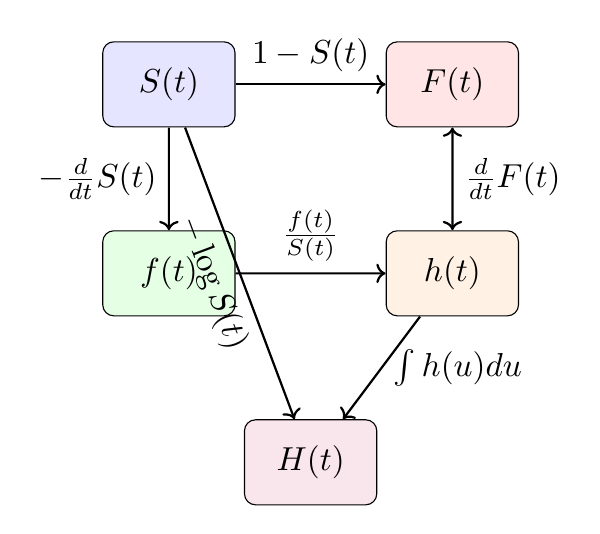
\begin{tikzpicture}[scale=1.2, transform shape]
        \node[draw, rounded corners, fill=blue!10, minimum width=1.4cm, minimum height=0.9cm] (S) at (0,0) {$S(t)$};
        \node[draw, rounded corners, fill=red!10, minimum width=1.4cm, minimum height=0.9cm] (F) at (3,0) {$F(t)$};
        \node[draw, rounded corners, fill=green!10, minimum width=1.4cm, minimum height=0.9cm] (f) at (0,-2) {$f(t)$};
        \node[draw, rounded corners, fill=orange!10, minimum width=1.4cm, minimum height=0.9cm] (h) at (3,-2) {$h(t)$};
        \node[draw, rounded corners, fill=purple!10, minimum width=1.4cm, minimum height=0.9cm] (H) at (1.5,-4) {$H(t)$};

        \draw[->, thick] (S) -- node[above] {$1-S(t)$} (F);
        \draw[<->, thick] (F) -- node[right] {$\frac{d}{dt}F(t)$} (h);
        \draw[->, thick] (S) -- node[left] {$-\frac{d}{dt}S(t)$} (f);
        \draw[->, thick] (S) -- node[below, sloped] {$-\log S(t)$} (H);
        \draw[->, thick] (f) -- node[above] {$\frac{f(t)}{S(t)}$} (h);
        \draw[->, thick] (h) -- node[right] {$\int h(u)du$} (H);
    \end{tikzpicture}
    \caption{Relationships between the core functions in survival analysis. Each function can be derived from the others through the transformations shown on the arrows.}
    \label{fig:survival-function-relationships}
\end{figure}

These mathematical relationships lead to several important practical formulas:

\begin{equationbox}[title=Key Mathematical Relationships]
\begin{align}
    S(t) &= \exp(-H(t)) = \exp\left(-\int_0^t h(u)du\right)\\
    f(t) &= h(t) \times S(t)\\
    h(t) &= \frac{f(t)}{S(t)} = -\frac{d}{dt}\log S(t)
\end{align}
\end{equationbox}

Understanding these relationships is crucial for model development and implementation. For example:
\begin{itemize}
    \item To derive a survival function from a specified hazard function, use $S(t) = \exp(-\int_0^t h(u)du)$
    \item To compute the density function when the hazard and survival are known, use $f(t) = h(t) \times S(t)$
    \item To estimate the hazard function from empirically derived survival estimates, use $h(t) = -\frac{d}{dt}\log S(t)$
\end{itemize}

The choice of which function to work with often depends on the specific application, computational considerations, and the specific modeling approach used.

\section{Understanding Hazard Functions}

The hazard function provides particularly valuable insights into the time-dependent risk profile. It helps identify the underlying mechanisms and patterns in time-to-event processes.

\subsection{Interpretation of the Hazard Function}

The hazard function $h(t)$ represents the instantaneous rate of failure at time $t$, given survival to time $t$. While it is not a probability (it can exceed 1), it can be interpreted as follows:

\begin{itemize}
    \item For small time intervals $\Delta t$, the quantity $h(t)\Delta t$ approximates the probability of the event occurring in the interval $(t, t+\Delta t]$, given survival to time $t$
    \item Higher values of $h(t)$ indicate greater instantaneous risk
    \item The shape of $h(t)$ over time reveals how risk evolves throughout the process
    \item Comparing hazard functions between groups shows relative risk over time
\end{itemize}

\begin{notebox}[title=Intuitive Interpretation]
While mathematically defined as a conditional rate, the hazard function can be intuitively understood as:
\begin{itemize}
    \item In medical contexts: The force of mortality or the propensity to fail at time $t$
    \item In engineering: The wear-out rate or proneness to failure at a specific point in a component's life
    \item In business: The customer's tendency to churn or cancel service at a given point in their lifecycle
\end{itemize}

The shape of the hazard function often provides clues about the underlying mechanisms driving the event process.
\end{notebox}

\subsection{Common Hazard Patterns}

Different processes exhibit characteristic hazard patterns that reflect their underlying mechanisms. Understanding these common patterns helps with model selection and interpretation.

\subsubsection{Constant Hazard}

The simplest hazard pattern is the constant hazard, where the instantaneous risk remains unchanged over time.

\begin{equationbox}[title=Constant Hazard Function]
\begin{equation}
    h(t) = \lambda \quad \text{for all } t \geq 0
\end{equation}

where $\lambda > 0$ is a constant rate parameter.

This leads to:
\begin{align}
    H(t) &= \lambda t\\
    S(t) &= \exp(-\lambda t)\\
    f(t) &= \lambda \exp(-\lambda t)
\end{align}
\end{equationbox}

\begin{figure}[htbp]
    \centering
    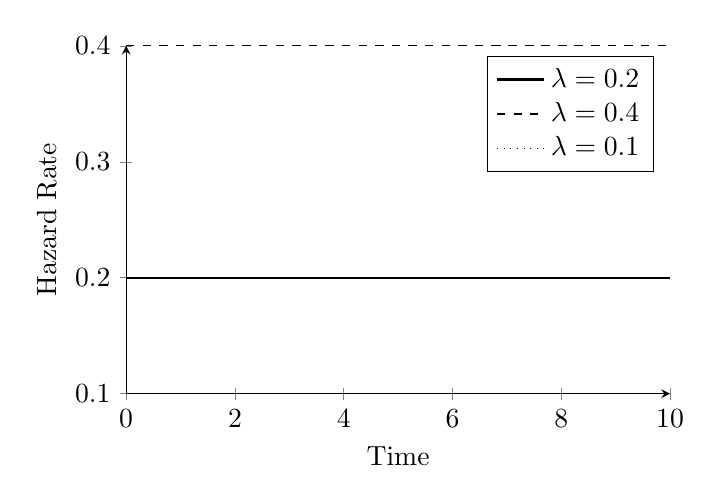
\begin{tikzpicture}
        \begin{axis}[
            width=0.7\textwidth,
            height=6cm,
            xlabel={Time},
            ylabel={Hazard Rate},
            axis lines=left,
            domain=0:10,
            samples=100,
            legend pos=north east,
          ]
          % Constant hazard (exponential)
          \addplot[black, thick] {0.2};
          \addplot[black, dashed] {0.4};
          \addplot[black, dotted] {0.1};
          \legend{$\lambda = 0.2$, $\lambda = 0.4$, $\lambda = 0.1$}
        \end{axis}
    \end{tikzpicture}
    \caption{Constant hazard functions with different rate parameters $\lambda$. A constant hazard indicates that the instantaneous risk remains stable over time, regardless of how long the subject has survived.}
    \label{fig:constant-hazard-rates}
\end{figure}

A constant hazard results in an exponential distribution for the event times. This distribution has the "memoryless" property, meaning that the future risk is independent of the past survival history.

\begin{examplebox}[title=Applications of Constant Hazard Models]
Constant hazard patterns are commonly observed in:
\begin{itemize}
    \item Random electronic component failures during their useful life period
    \item Occurrence of accidents unrelated to age or wear
    \item Events driven by random environmental factors
    \item Radioactive decay processes
    \item Some chronic disease mortality in middle age ranges
\end{itemize}

The constant hazard assumption is often used as a baseline or null model against which to compare more complex hazard patterns.
\end{examplebox}

\subsubsection{Monotonically Increasing Hazard}

Many real-world processes show increasing risk over time, reflecting aging, wear, or accumulating damage.

\begin{equationbox}[title=Weibull Increasing Hazard]
A flexible model for increasing hazard is the Weibull distribution with shape parameter $k > 1$:
\begin{equation}
    h(t) = \frac{k}{\lambda}\left(\frac{t}{\lambda}\right)^{k-1}
\end{equation}

where $k > 1$ is the shape parameter and $\lambda > 0$ is the scale parameter.
\end{equationbox}

\begin{figure}[htbp]
    \centering
    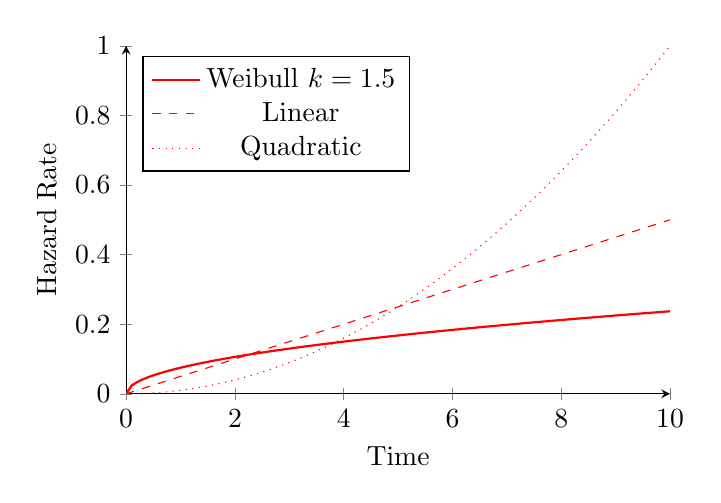
\begin{tikzpicture}
        \begin{axis}[
            width=0.7\textwidth,
            height=6cm,
            xlabel={Time},
            ylabel={Hazard Rate},
            axis lines=left,
            domain=0:10,
            samples=100,
            legend pos=north west,
          ]
          % Increasing hazards with different parameters
          \addplot[red, thick] {0.075*x^0.5};
          \addplot[red, dashed] {0.05*x^1.0};
          \addplot[red, dotted] {0.01*x^2.0};
          \legend{Weibull $k=1.5$, Linear, Quadratic}
        \end{axis}
    \end{tikzpicture}
    \caption{Monotonically increasing hazard functions. These patterns indicate that risk increases with time, which is characteristic of aging, wear-out, and progressive deterioration processes.}
    \label{fig:increasing-hazard}
\end{figure}

Increasing hazards are particularly common in:
\begin{itemize}
    \item Aging processes in living organisms
    \item Mechanical wear and fatigue failures
    \item Progressive diseases where condition worsens over time
    \item Cancer recurrence risk after initial treatment
    \item Systems with cumulative damage
\end{itemize}

The rate of increase in the hazard reflects the speed of deterioration or aging in the underlying process.

\subsubsection{Monotonically Decreasing Hazard}

Some processes exhibit decreasing risk over time, often reflecting initial vulnerability followed by increasing stability.

\begin{equationbox}[title=Weibull Decreasing Hazard]
The Weibull distribution with shape parameter $k < 1$ produces a decreasing hazard:
\begin{equation}
    h(t) = \frac{k}{\lambda}\left(\frac{t}{\lambda}\right)^{k-1}
\end{equation}

where $0 < k < 1$ is the shape parameter and $\lambda > 0$ is the scale parameter.
\end{equationbox}

\begin{figure}[htbp]
    \centering
    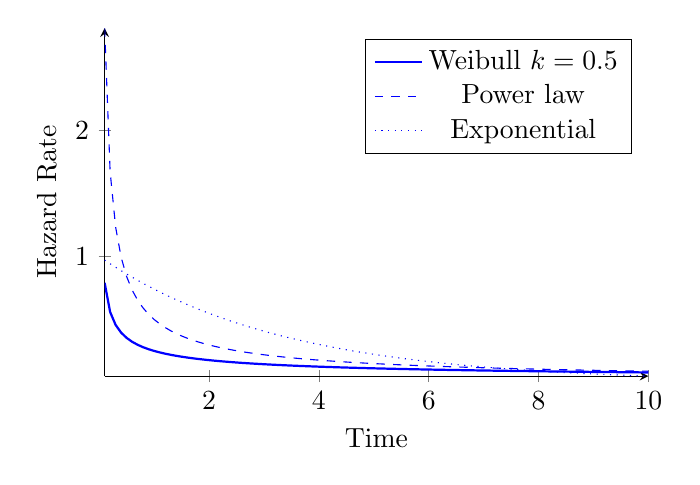
\begin{tikzpicture}
        \begin{axis}[
            width=0.7\textwidth,
            height=6cm,
            xlabel={Time},
            ylabel={Hazard Rate},
            axis lines=left,
            domain=0.1:10,
            samples=100,
            legend pos=north east,
          ]
          % Decreasing hazards with different parameters
          \addplot[blue, thick] {0.25*x^(-0.5)};
          \addplot[blue, dashed] {0.5*x^(-0.75)};
          \addplot[blue, dotted] {1.0*exp(-0.3*x)};
          \legend{Weibull $k=0.5$, Power law, Exponential}
        \end{axis}
    \end{tikzpicture}
    \caption{Monotonically decreasing hazard functions. These patterns show risk diminishing with time, which can indicate early vulnerability followed by strengthening or stabilization.}
    \label{fig:decreasing-hazard}
\end{figure}

Decreasing hazards appear in:
\begin{itemize}
    \item Infant mortality in humans and early failure in manufacturing
    \item Post-surgical infection risk, which is highest immediately after surgery
    \item Treatment efficacy that diminishes over time
    \item Immune response development after exposure
    \item Systems that strengthen or stabilize with time
\end{itemize}

Decreasing hazards often reflect selection processes where weaker subjects fail early, leaving a progressively more robust population.

\subsubsection{Non-Monotonic Hazard Patterns}

Many real-world processes exhibit more complex hazard patterns that combine elements of increasing and decreasing hazards.

\paragraph{Bathtub-Shaped Hazard}

The bathtub-shaped hazard curve starts high, decreases to a relatively stable level, and then increases again at later times.

\begin{figure}[htbp]
    \centering
    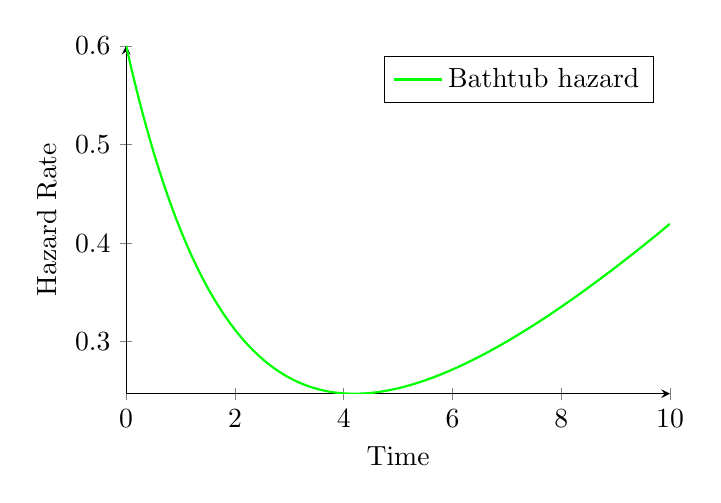
\begin{tikzpicture}
        \begin{axis}[
            width=0.7\textwidth,
            height=6cm,
            xlabel={Time},
            ylabel={Hazard Rate},
            axis lines=left,
            domain=0:10,
            samples=100,
            legend pos=north east,
          ]
          % Bathtub hazard
          \addplot[green, thick] {0.5*exp(-0.5*x) + 0.1 + 0.01*x^(1.5)};
          \legend{Bathtub hazard}
        \end{axis}
    \end{tikzpicture}
    \caption{Bathtub-shaped hazard function showing high initial risk, followed by a period of relative stability, and ending with increasing risk. This pattern is common in human mortality and complex system lifecycles.}
    \label{fig:bathtub-hazard}
\end{figure}

This pattern commonly appears in:
\begin{itemize}
    \item Human mortality across the lifespan (infant mortality, stable adulthood, aging)
    \item Complete product lifecycles (early defects, useful life, wear-out)
    \item Systems with multiple failure modes operating at different time scales
\end{itemize}

\paragraph{Hump-Shaped Hazard}

Hump-shaped (or unimodal) hazards start low, increase to a peak, and then decrease again.

\begin{figure}[htbp]
    \centering
    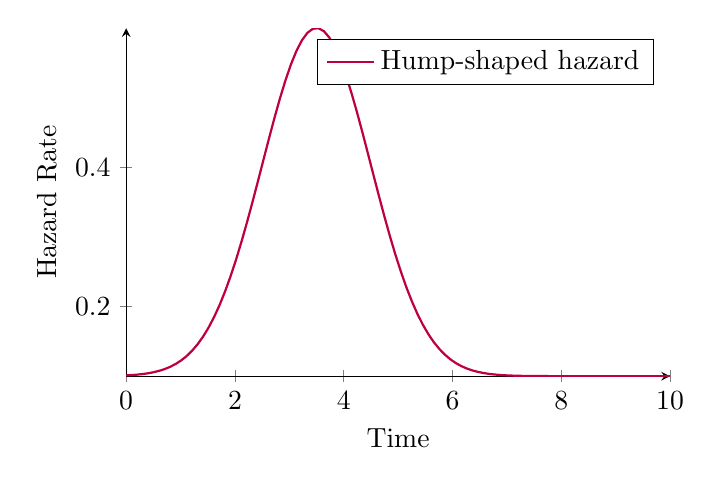
\begin{tikzpicture}
        \begin{axis}[
            width=0.7\textwidth,
            height=6cm,
            xlabel={Time},
            ylabel={Hazard Rate},
            axis lines=left,
            domain=0:10,
            samples=100,
            legend pos=north east,
          ]
          % Hump-shaped hazard
          \addplot[purple, thick] {0.1 + 0.5*exp(-(x-3.5)^2/2)};
          \legend{Hump-shaped hazard}
        \end{axis}
    \end{tikzpicture}
    \caption{Hump-shaped hazard function showing risk that increases to a peak and then decreases. This pattern often occurs in scenarios with a critical time window of vulnerability.}
    \label{fig:hump-hazard}
\end{figure}

This pattern is common in:
\begin{itemize}
    \item Post-surgical complications that peak during a critical recovery phase
    \item Treatment response patterns with a window of vulnerability
    \item Certain diseases with age-specific incidence peaks
    \item Log-normal failure distributions
\end{itemize}

\subsection{Hazard Patterns in Real-World Applications}

Recognizing hazard patterns in real data helps identify appropriate models and understand underlying mechanisms.

\subsubsection{Medical Applications}

Different medical conditions exhibit characteristic hazard patterns:
\begin{itemize}
    \item \textbf{Cancer progression:} Often shows increasing hazard as the disease advances and becomes more aggressive
    \item \textbf{Post-surgery recovery:} Typically shows high initial risk from complications, followed by declining risk
    \item \textbf{Infectious diseases:} May show hump-shaped hazards with peak risk during specific phases
    \item \textbf{Chronic conditions:} Often exhibit slowly increasing hazards reflecting progressive nature
\end{itemize}

\subsubsection{Engineering Applications}

Mechanical and electronic systems often follow well-established hazard patterns:
\begin{itemize}
    \item \textbf{Electronic components:} Often follow the bathtub curve with three distinct phases:
    \begin{itemize}
        \item Early failures due to manufacturing defects (decreasing hazard)
        \item Random failures during useful life (constant hazard)
        \item Wear-out failures in later life (increasing hazard)
    \end{itemize}
    \item \textbf{Mechanical systems:} Frequently show increasing hazards due to wear, fatigue, or corrosion
    \item \textbf{Complex systems:} May exhibit mixture patterns reflecting multiple components and failure modes
\end{itemize}

\begin{notebox}[title=Implications for Modeling]
Understanding the hazard pattern of a process provides crucial guidance for model selection:
\begin{itemize}
    \item Constant hazard processes are well-modeled by exponential distributions
    \item Monotonically changing hazards often fit well with Weibull distributions
    \item Non-monotonic hazards may require mixture models or more flexible parametric forms
    \item Complex patterns might benefit from non-parametric or semi-parametric approaches
\end{itemize}

Misspecification of the hazard pattern can lead to poor model fit and misleading conclusions.
\end{notebox}

\section{Censoring in Survival Analysis}

Censoring—the partial observation of event times—is a defining characteristic of survival data that requires specialized analytical methods. The detailed discussion of censoring, its types, and mechanisms can be found in Chapter \ref{ch:censoring}.

\subsection{Truncation vs. Censoring}

It's important to distinguish between censoring and truncation, as they represent fundamentally different data limitations.

\begin{definitionbox}[title=Truncation]
Truncation occurs when subjects are systematically excluded from the sample based on their event times. Unlike censoring (which is partial observation), truncation means complete exclusion of certain subjects.

\begin{itemize}
    \item \textbf{Left truncation:} Subjects are only included if their event time exceeds some threshold ($T > L$)
    \item \textbf{Right truncation:} Subjects are only included if their event time is less than some threshold ($T < R$)
\end{itemize}
\end{definitionbox}

Examples of truncation include:
\begin{itemize}
    \item Studies of disease duration that recruit patients who already have the disease (left truncation)
    \item Studies based on death records, which only include those who have died (right truncation)
    \item Age-specific studies that only include subjects within certain age ranges
\end{itemize}

Truncation creates a biased sample and requires special methods to correct for the bias in estimation.

\section{Likelihood Functions for Survival Data}

The likelihood function serves as the foundation for parameter estimation in survival analysis. Due to censoring, the standard likelihood approach must be adapted to handle partially observed data.

\subsection{General Principles of Likelihood Functions}

In standard statistics, the likelihood function measures the consistency between observed data and a particular set of model parameters:

\begin{equationbox}[title=Standard Likelihood Function]
For observations $X = \{x_1, x_2, \ldots, x_n\}$ and parameters $\theta$:
\begin{equation}
    \mathcal{L}(\theta | X) = p(X | \theta) = \prod_{i=1}^{n} p(x_i | \theta)
\end{equation}

where $p(x_i | \theta)$ is the probability density function for observation $x_i$.
\end{equationbox}

Maximum likelihood estimation (MLE) seeks the parameter values that maximize this likelihood:
\begin{equation}
    \hat{\theta}_{MLE} = \arg\max_{\theta} \mathcal{L}(\theta | X)
\end{equation}

For computational convenience, we often maximize the log-likelihood instead:
\begin{equation}
    \hat{\theta}_{MLE} = \arg\max_{\theta} \log\mathcal{L}(\theta | X) = \arg\max_{\theta} \sum_{i=1}^{n} \log p(x_i | \theta)
\end{equation}

\subsection{Survival Likelihood with Censoring}

In survival analysis, we observe a mixture of exact event times and censored observations. Each type contributes differently to the likelihood.

\begin{equationbox}[title=Survival Likelihood with Right Censoring]
For a dataset with $n$ subjects, each characterized by $(y_i, \delta_i)$ where $y_i$ is the observed time and $\delta_i$ is the event indicator:
\begin{equation}
    \mathcal{L}(\theta) = \prod_{i=1}^{n} [f(y_i|\theta)]^{\delta_i} [S(y_i|\theta)]^{1-\delta_i}
\end{equation}

where:
\begin{itemize}
    \item For observed events ($\delta_i = 1$): Contribution is $f(y_i|\theta)$, the density at the exact time
    \item For censored observations ($\delta_i = 0$): Contribution is $S(y_i|\theta)$, the probability of surviving beyond the censoring time
\end{itemize}
\end{equationbox}

This formulation elegantly handles both types of observations by using the event indicator $\delta_i$ to select the appropriate term for each subject.

\begin{figure}[htbp]
    \centering
    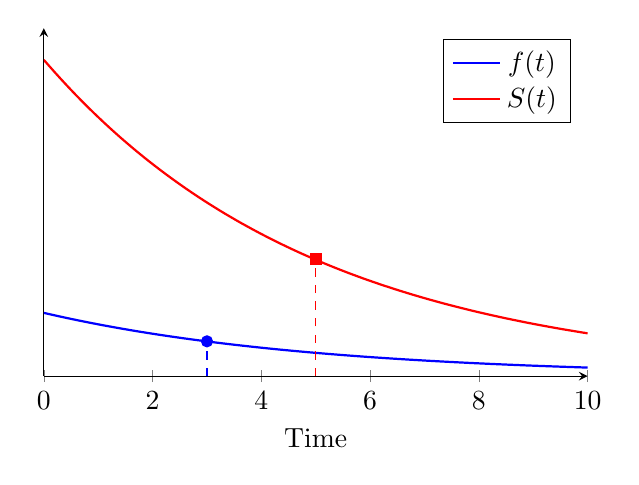
\begin{tikzpicture}
        \begin{axis}[
            width=0.7\textwidth,
            height=6cm,
            xlabel={Time},
            ylabel={},
            axis lines=left,
            domain=0:10,
            ytick=\empty,
            yticklabels={},
            ymin=0, ymax=1.1,
            legend pos=north east,
          ]

          % Density function
          \addplot[blue, thick, domain=0:10, samples=100] {0.2*exp(-0.2*x)};

          % Survival function
          \addplot[red, thick, domain=0:10, samples=100] {exp(-0.2*x)};

          % Observed event (use density)
          \addplot[blue, mark=*, only marks] coordinates {(3, 0.11)};
          \draw[blue, dashed] (axis cs:3,0) -- (axis cs:3,0.11);
          \node[blue] at (axis cs:3,-0.05) {$t_1$};

          % Censored observation (use survival)
          \addplot[red, mark=square*, only marks] coordinates {(5, 0.37)};
          \draw[red, dashed] (axis cs:5,0) -- (axis cs:5,0.37);
          \node[red] at (axis cs:5,-0.05) {$c_2$};

          \legend{$f(t)$,$S(t)$}
        \end{axis}
    \end{tikzpicture}
    \caption{Likelihood contributions for different observation types. For observed events (blue), the contribution is the density $f(t)$ at the exact event time. For censored observations (red), the contribution is the survival function $S(t)$ at the censoring time.}
    \label{fig:likelihood-contributions}
\end{figure}

\subsection{Alternative Formulations}

Using the relationship $f(t) = h(t)S(t)$, we can rewrite the likelihood in terms of the hazard function:

\begin{equationbox}[title=Hazard-Based Likelihood]
\begin{align}
    \mathcal{L}(\theta) &= \prod_{i=1}^{n} [h(y_i|\theta)S(y_i|\theta)]^{\delta_i} [S(y_i|\theta)]^{1-\delta_i} \\
    &= \prod_{i=1}^{n} [h(y_i|\theta)]^{\delta_i} S(y_i|\theta)
\end{align}
\end{equationbox}

Taking the logarithm and using $S(t) = \exp(-H(t))$, we obtain the log-likelihood:

\begin{equationbox}[title=Log-Likelihood for Survival Data]
\begin{align}
    \log\mathcal{L}(\theta) &= \sum_{i=1}^{n} \delta_i \log h(y_i|\theta) + \sum_{i=1}^{n} \log S(y_i|\theta) \\
    &= \sum_{i=1}^{n} \delta_i \log h(y_i|\theta) - \sum_{i=1}^{n} H(y_i|\theta)
\end{align}
\end{equationbox}

This formulation is particularly useful for model development and implementation, as it separates the components related to observed events (first term) and the risk accumulated by all subjects (second term).

\subsection{Handling Other Types of Censoring}

While the likelihood for right-censored data is most common, other types of censoring require different likelihood formulations:

\begin{itemize}
    \item \textbf{Left censoring:} For a left-censored observation at time $c$, the contribution is $F(c|\theta)$, the probability of the event occurring before time $c$

    \item \textbf{Interval censoring:} For an observation known to occur in the interval $(L, R)$, the contribution is $F(R|\theta) - F(L|\theta)$, the probability of the event occurring within the interval

    \item \textbf{Mixed censoring:} When different observations have different censoring types, each contributes appropriately according to its type
\end{itemize}

\begin{examplebox}[title=General Likelihood with Multiple Censoring Types]
For a dataset with right-censored, left-censored, and interval-censored observations:
\begin{align}
    \mathcal{L}(\theta) = \prod_{i \in \mathcal{R}} f(y_i|\theta) \prod_{j \in \mathcal{L}} F(y_j|\theta) \prod_{k \in \mathcal{I}} [F(R_k|\theta) - F(L_k|\theta)] \prod_{l \in \mathcal{C}} S(y_l|\theta)
\end{align}

where $\mathcal{R}$, $\mathcal{L}$, $\mathcal{I}$, and $\mathcal{C}$ represent the sets of exact, left-censored, interval-censored, and right-censored observations, respectively.
\end{examplebox}

\section{Non-Parametric Survival Estimation}

Non-parametric methods make minimal assumptions about the underlying distribution of survival times, providing flexible descriptive analyses of survival patterns.

\subsection{The Kaplan-Meier Estimator}

The Kaplan-Meier estimator (also called the product-limit estimator) is the most widely used non-parametric approach for estimating the survival function from right-censored data.

\begin{definitionbox}[title=Kaplan-Meier Estimator]
For a dataset with observed times $t_1 < t_2 < \cdots < t_k$, the Kaplan-Meier estimator of the survival function is:
\begin{equation}
    \hat{S}(t) = \prod_{i: t_i \leq t} \left(1 - \frac{d_i}{n_i}\right)
\end{equation}

where:
\begin{itemize}
    \item $d_i$ is the number of events at time $t_i$
    \item $n_i$ is the number of subjects at risk just before time $t_i$
    \item $\left(1 - \frac{d_i}{n_i}\right)$ represents the conditional probability of surviving through the interval containing $t_i$
\end{itemize}
\end{definitionbox}

The Kaplan-Meier estimator has several important properties:
\begin{itemize}
    \item It is a step function that decreases only at observed event times
    \item It is the non-parametric maximum likelihood estimator for the survival function
    \item It properly accounts for right-censored observations
    \item It does not require specification of the underlying distribution
\end{itemize}

\begin{figure}[htbp]
    \centering
    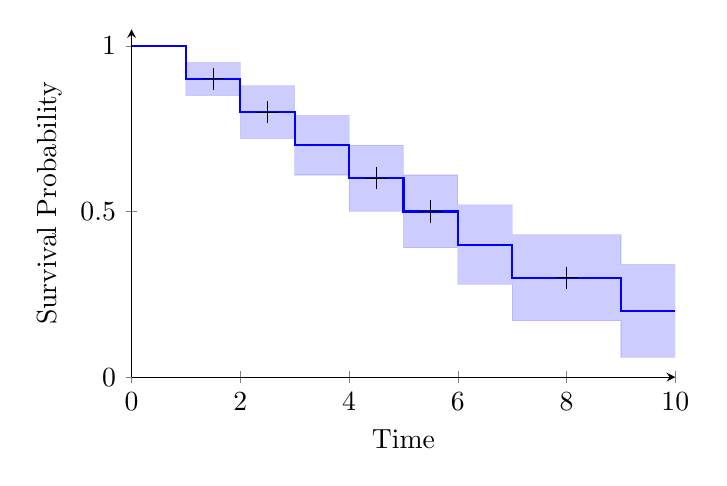
\begin{tikzpicture}
        \begin{axis}[
            width=0.7\textwidth,
            height=6cm,
            xlabel={Time},
            ylabel={Survival Probability},
            axis lines=left,
            xmin=0, xmax=10,
            ymin=0, ymax=1.05,
          ]
          % Kaplan-Meier step function
          \addplot[const plot, blue, thick, mark=none] coordinates {
            (0, 1.0) (1, 1.0) (1, 0.9) (2, 0.9) (2, 0.8)
            (3, 0.8) (3, 0.7) (4, 0.7) (4, 0.6) (5, 0.6)
            (5, 0.5) (6, 0.5) (6, 0.4) (7, 0.4) (7, 0.3)
            (9, 0.3) (9, 0.2) (10, 0.2)
          };

          % Confidence intervals
          \addplot[name path=upper, blue, opacity=0.1] coordinates {
            (0, 1.0) (1, 1.0) (1, 0.95) (2, 0.95) (2, 0.88)
            (3, 0.88) (3, 0.79) (4, 0.79) (4, 0.7) (5, 0.7)
            (5, 0.61) (6, 0.61) (6, 0.52) (7, 0.52) (7, 0.43)
            (9, 0.43) (9, 0.34) (10, 0.34)
          };

          \addplot[name path=lower, blue, opacity=0.1] coordinates {
            (0, 1.0) (1, 1.0) (1, 0.85) (2, 0.85) (2, 0.72)
            (3, 0.72) (3, 0.61) (4, 0.61) (4, 0.5) (5, 0.5)
            (5, 0.39) (6, 0.39) (6, 0.28) (7, 0.28) (7, 0.17)
            (9, 0.17) (9, 0.06) (10, 0.06)
          };

          \addplot[blue, fill opacity=0.2] fill between[of=upper and lower];

          % Add + marks for censored observations
          \addplot[only marks, mark=+, mark size=4pt, black] coordinates {
            (1.5, 0.9) (2.5, 0.8) (4.5, 0.6) (5.5, 0.5) (8, 0.3)
          };
        \end{axis}
    \end{tikzpicture}
    \caption{Kaplan-Meier estimate of the survival function with 95\% confidence intervals. The step function decreases only at observed event times, while + marks indicate censored observations. The confidence intervals (shaded region) widen over time as information decreases.}
    \label{fig:km-estimate-with-ci}
\end{figure}

\subsubsection{Confidence Intervals for Kaplan-Meier Estimates}

Greenwood's formula provides a variance estimator for the Kaplan-Meier estimate:

\begin{equationbox}[title=Greenwood's Formula]
\begin{equation}
    \text{Var}[\hat{S}(t)] = [\hat{S}(t)]^2 \sum_{i: t_i \leq t} \frac{d_i}{n_i(n_i-d_i)}
\end{equation}
\end{equationbox}

A 95\% confidence interval for the survival function at time $t$ can be constructed as:
\begin{equation}
    \hat{S}(t) \pm 1.96 \sqrt{\text{Var}[\hat{S}(t)]}
\end{equation}

Alternative formulations, such as the log-log transformation, are sometimes used to ensure the confidence limits remain within the range $[0, 1]$ and to improve the approximation for small samples.

\subsection{Nelson-Aalen Estimator}

While the Kaplan-Meier estimator focuses on the survival function, the Nelson-Aalen estimator provides a non-parametric estimate of the cumulative hazard function.

\begin{definitionbox}[title=Nelson-Aalen Estimator]
The Nelson-Aalen estimator of the cumulative hazard function is:
\begin{equation}
    \hat{H}(t) = \sum_{i: t_i \leq t} \frac{d_i}{n_i}
\end{equation}

where $d_i$ and $n_i$ are defined as in the Kaplan-Meier estimator.
\end{definitionbox}

The Nelson-Aalen estimator provides a basis for:
\begin{itemize}
    \item Estimating the cumulative hazard directly
    \item Examining temporal patterns in hazard rates
    \item Checking model assumptions
    \item Deriving an alternative estimator of the survival function:
    \begin{equation}
        \hat{S}_{NA}(t) = \exp(-\hat{H}(t))
    \end{equation}
\end{itemize}

\subsection{Comparing Groups with Non-Parametric Methods}

Non-parametric methods are particularly valuable for comparing survival between groups without assuming specific distributional forms.

\subsubsection{Log-Rank Test}

The log-rank test is the most widely used method for comparing two or more survival curves.

\begin{definitionbox}[title=Log-Rank Test]
The log-rank test compares observed versus expected events in each group under the null hypothesis of equal survival functions.

For $G$ groups, the test statistic is:
\begin{equation}
    \chi^2 = \sum_{j=1}^{G} \frac{(O_j - E_j)^2}{E_j}
\end{equation}

where $O_j$ is the observed number of events in group $j$, and $E_j$ is the expected number under the null hypothesis.

Under the null hypothesis, this statistic follows a chi-square distribution with $G-1$ degrees of freedom.
\end{definitionbox}

The log-rank test is most powerful for detecting differences when the hazard ratios between groups are constant over time (i.e., when the proportional hazards assumption holds).

\subsubsection{Weighted Log-Rank Tests}

Various weighted versions of the log-rank test give different emphasis to early or late differences in survival:
\begin{itemize}
    \item \textbf{Gehan-Breslow test:} Weights by the number at risk, giving more emphasis to early differences
    \item \textbf{Tarone-Ware test:} Uses square root of the number at risk as weights
    \item \textbf{Peto-Peto test:} Weights by a modified survival estimate, reducing the influence of late differences where data are sparse
\end{itemize}

\begin{figure}[htbp]
    \centering
    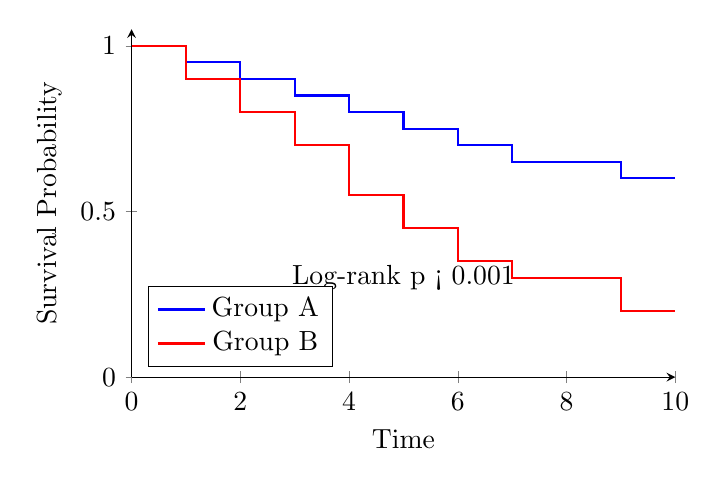
\begin{tikzpicture}
        \begin{axis}[
            width=0.7\textwidth,
            height=6cm,
            xlabel={Time},
            ylabel={Survival Probability},
            axis lines=left,
            xmin=0, xmax=10,
            ymin=0, ymax=1.05,
            legend pos=south west,
          ]
          % Group A
          \addplot[const plot, blue, thick, mark=none] coordinates {
            (0, 1.0) (1, 1.0) (1, 0.95) (2, 0.95) (2, 0.9)
            (3, 0.9) (3, 0.85) (4, 0.85) (4, 0.8) (5, 0.8)
            (5, 0.75) (6, 0.75) (6, 0.7) (7, 0.7) (7, 0.65)
            (9, 0.65) (9, 0.6) (10, 0.6)
          };

          % Group B
          \addplot[const plot, red, thick, mark=none] coordinates {
            (0, 1.0) (1, 1.0) (1, 0.9) (2, 0.9) (2, 0.8)
            (3, 0.8) (3, 0.7) (4, 0.7) (4, 0.55) (5, 0.55)
            (5, 0.45) (6, 0.45) (6, 0.35) (7, 0.35) (7, 0.3)
            (9, 0.3) (9, 0.2) (10, 0.2)
          };

          \legend{Group A, Group B}

          % Display p-value
          \node at (axis cs:5,0.3) {Log-rank p < 0.001};
        \end{axis}
    \end{tikzpicture}
    \caption{Kaplan-Meier curves comparing survival between two groups, with the log-rank test result indicating a significant difference.}
    \label{fig:km-comparison}
\end{figure}

\section{The Cox Proportional Hazards Model}

The Cox proportional hazards model is the most widely used approach for analyzing the effect of covariates on survival time. It represents a semi-parametric approach that balances flexibility with the ability to perform covariate adjustment.

\subsection{Model Formulation}

\begin{definitionbox}[title=Cox Proportional Hazards Model]
The Cox model specifies the hazard function for an individual with covariate vector $X$ as:
\begin{equation}
    h(t|X) = h_0(t) \exp(X\beta)
\end{equation}

where:
\begin{itemize}
    \item $h_0(t)$ is the baseline hazard function (left unspecified)
    \item $X$ is the vector of covariates
    \item $\beta$ is the vector of regression coefficients
    \item $\exp(X\beta)$ is the hazard ratio relative to baseline
\end{itemize}
\end{definitionbox}

This model has several notable features:
\begin{itemize}
    \item It makes no assumptions about the shape of the baseline hazard $h_0(t)$
    \item The effect of covariates is multiplicative on the hazard scale
    \item The hazard ratio $\exp(X\beta)$ is constant over time (the proportional hazards assumption)
    \item The log hazard is a linear function of the covariates
\end{itemize}

\subsection{Partial Likelihood Estimation}

A key innovation of the Cox model is the partial likelihood approach, which allows estimation of $\beta$ without specifying the baseline hazard $h_0(t)$.

\begin{definitionbox}[title=Partial Likelihood]
The partial likelihood for the Cox model is:
\begin{equation}
    PL(\beta) = \prod_{i: \delta_i=1} \frac{\exp(X_i\beta)}{\sum_{j \in R(t_i)}\exp(X_j\beta)}
\end{equation}

where:
\begin{itemize}
    \item The product is over observed events (not censored observations)
    \item $R(t_i)$ is the risk set at time $t_i$ (subjects still at risk just before $t_i$)
    \item The numerator represents the hazard for the subject who experienced the event
    \item The denominator sums the hazards across all subjects at risk at that time
\end{itemize}
\end{definitionbox}

The partial likelihood depends only on the order of events, not their exact timing, and eliminates the baseline hazard. Maximizing this partial likelihood yields consistent estimates of $\beta$ under the proportional hazards assumption.

\subsection{Interpretation of Parameters}

The coefficients in the Cox model have a direct hazard ratio interpretation:

\begin{examplebox}[title=Interpreting Cox Model Coefficients]
For a coefficient $\beta_j$ corresponding to covariate $X_j$:
\begin{itemize}
    \item $\exp(\beta_j)$ is the hazard ratio for a one-unit increase in $X_j$, holding other covariates constant
    \item $\beta_j > 0$ (or $\exp(\beta_j) > 1$) indicates increased hazard (worse survival)
    \item $\beta_j < 0$ (or $\exp(\beta_j) < 1$) indicates decreased hazard (better survival)
    \item $\beta_j = 0$ (or $\exp(\beta_j) = 1$) indicates no effect on hazard
\end{itemize}

Example: If $\beta_j = 0.693$ (so $\exp(\beta_j) = 2$), then a one-unit increase in $X_j$ is associated with a doubling of the hazard rate.
\end{examplebox}

\subsection{Baseline Hazard Estimation}

After estimating $\beta$, we can estimate the baseline hazard non-parametrically using the Breslow estimator:

\begin{equationbox}[title=Breslow Estimator]
\begin{equation}
    \hat{H}_0(t) = \sum_{i: t_i \leq t} \frac{d_i}{\sum_{j \in R(t_i)} \exp(X_j\hat{\beta})}
\end{equation}

where $d_i$ is the number of events at time $t_i$.
\end{equationbox}

From this, we can derive the baseline survival function:
\begin{equation}
    \hat{S}_0(t) = \exp(-\hat{H}_0(t))
\end{equation}

And the individual survival function for a subject with covariates $X$:
\begin{equation}
    \hat{S}(t|X) = [\hat{S}_0(t)]^{\exp(X\hat{\beta})}
\end{equation}

\subsection{Extensions of the Cox Model}

Several extensions address limitations of the basic Cox model:

\subsubsection{Time-Dependent Covariates}

The Cox model can accommodate covariates that change over time:
\begin{equation}
    h(t|X(t)) = h_0(t) \exp(X(t)\beta)
\end{equation}

Examples include:
\begin{itemize}
    \item Biomarkers that change during follow-up
    \item Treatment status that changes over time
    \item Environmental exposures that vary temporally
\end{itemize}

\subsubsection{Stratified Cox Model}

When the proportional hazards assumption holds within groups but not across groups, the stratified Cox model allows different baseline hazards for each stratum:
\begin{equation}
    h(t|X, s) = h_{0s}(t) \exp(X\beta)
\end{equation}

where $s$ indexes the stratum and $h_{0s}(t)$ is the stratum-specific baseline hazard.

\subsubsection{Frailty Models}

Frailty models account for unobserved heterogeneity and clustered data by introducing random effects:
\begin{equation}
    h(t|X, Z) = h_0(t) \exp(X\beta + Z)
\end{equation}

where $Z$ represents unobserved frailty (random effect) that induces correlation within clusters.

\section{Competing Risks Analysis}

Competing risks occur when subjects can experience different types of events, where the occurrence of one event precludes observation of others. A detailed discussion of competing risks can be found in Chapter \ref{ch:censoring}.

\subsection{Framework and Terminology}

In a competing risks setting, we observe:
\begin{itemize}
    \item The time to the first event: $T = \min(T_1, T_2, \ldots, T_K)$
    \item The type of the first event: $J \in \{1, 2, \ldots, K\}$
    \item Possibly right-censoring: $C$
\end{itemize}

We observe $(Y, \delta, J)$ where:
\begin{itemize}
    \item $Y = \min(T, C)$ is the observed time
    \item $\delta = I(T \leq C)$ indicates whether an event was observed
    \item $J$ indicates the type of event (when $\delta = 1$)
\end{itemize}

\subsection{Key Functions in Competing Risks}

\begin{definitionbox}[title=Cause-Specific Hazard]
The cause-specific hazard for event type $j$ is:
\begin{equation}
    h_j(t) = \lim_{\Delta t \to 0} \frac{P(t \leq T < t + \Delta t, J = j | T \geq t)}{\Delta t}
\end{equation}

This represents the instantaneous risk of event type $j$ at time $t$, given survival until time $t$.
\end{definitionbox}

\begin{definitionbox}[title=Cumulative Incidence Function]
The cumulative incidence function (CIF) for event type $j$ is:
\begin{equation}
    F_j(t) = P(T \leq t, J = j) = \int_0^t S(u) h_j(u) du
\end{equation}

where $S(t) = \exp(-\sum_{k=1}^{K}\int_0^t h_k(u)du)$ is the overall survival function.

The CIF represents the probability of experiencing event type $j$ by time $t$, accounting for the fact that other event types can occur.
\end{definitionbox}

\subsection{Modeling Approaches for Competing Risks}

Two main modeling approaches are used for competing risks:

\subsubsection{Cause-Specific Hazards Approach}

This approach models each cause-specific hazard separately, typically using Cox regression:
\begin{equation}
    h_j(t|X) = h_{0j}(t) \exp(X\beta_j)
\end{equation}

Each event type has its own baseline hazard and regression coefficients, reflecting potentially different risk factors. This approach is useful for understanding the effect of covariates on the instantaneous risk of each event type.

\subsubsection{Fine-Gray Subdistribution Hazards Approach}

The Fine-Gray approach models the subdistribution hazard directly:
\begin{equation}
    \lambda_j(t|X) = \lambda_{0j}(t) \exp(X\gamma_j)
\end{equation}

where the subdistribution hazard is defined as:
\begin{equation}
    \lambda_j(t) = \lim_{\Delta t \to 0} \frac{P(t \leq T < t + \Delta t, J = j | T \geq t \cup (T \leq t \cap J \neq j))}{\Delta t}
\end{equation}

This approach models the CIF directly and is particularly useful for risk prediction and prognostic modeling.

\begin{figure}[htbp]
    \centering
    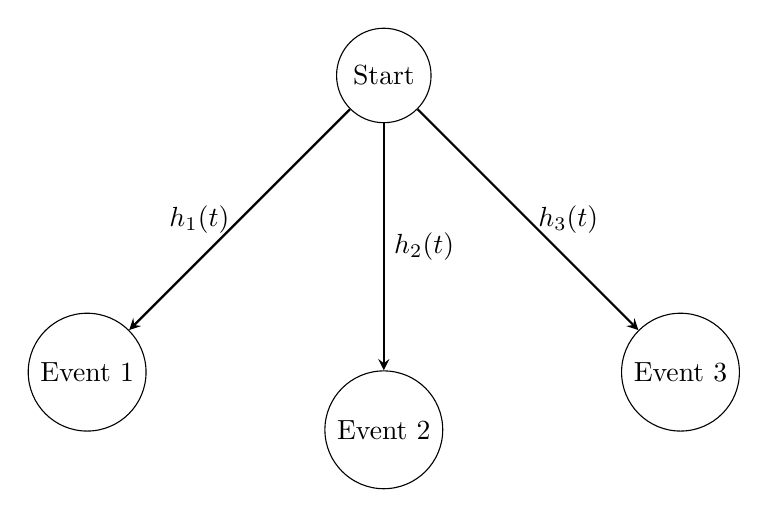
\begin{tikzpicture}[
        node distance=2.5cm,
        state/.style={circle, draw, minimum size=1.2cm},
        arrow/.style={->, >=stealth, thick}
    ]
        % States
        \node[state] (start) at (0,0) {Start};
        \node[state, below left of=start] (event1) at (-2,-2) {Event 1};
        \node[state, below of=start] (event2) at (0,-2) {Event 2};
        \node[state, below right of=start] (event3) at (2,-2) {Event 3};

        % Transitions
        \draw[arrow] (start) -- (event1) node[midway, left] {$h_1(t)$};
        \draw[arrow] (start) -- (event2) node[midway, right] {$h_2(t)$};
        \draw[arrow] (start) -- (event3) node[midway, right] {$h_3(t)$};
    \end{tikzpicture}
    \caption{Example of a competing risks model. From the initial state, a subject can transition to one of several possible event states, each with its own hazard function.}
    \label{fig:competing-risks-model}
\end{figure}

\section{Limitations of Classical Methods}

While classical survival analysis methods have proven invaluable across many domains, they have significant limitations, particularly for complex data and modern applications.

\subsection{Limitations of Parametric Models}

Parametric models make strong assumptions about the underlying distribution of survival times:
\begin{itemize}
    \item \textbf{Restrictive distributional assumptions:} Real-world data often do not conform to standard parametric families
    \item \textbf{Difficulty modeling complex hazard patterns:} Multi-modal or highly variable hazard shapes may not be well-approximated
    \item \textbf{Sensitivity to outliers:} Parameter estimates can be strongly influenced by extreme observations
    \item \textbf{Limited flexibility:} Fixed functional forms constrain how covariates affect survival
\end{itemize}

\subsection{Limitations of the Cox Model}

Despite its flexibility, the Cox model has several important limitations:
\begin{itemize}
    \item \textbf{Proportional hazards assumption:} The hazard ratio between any two subjects is assumed constant over time, which is often violated
    \item \textbf{Linear functional form:} Covariates are assumed to have a log-linear effect on the hazard, which may not capture complex relationships
    \item \textbf{Limited ability to model interactions:} Interactions must be pre-specified and are typically limited to low-order terms
    \item \textbf{Challenges with high-dimensional data:} The traditional Cox model is not designed for settings where the number of predictors exceeds the number of observations
\end{itemize}

\subsection{Limitations in Competing Risks Analysis}

Traditional competing risks approaches have their own challenges:
\begin{itemize}
    \item \textbf{Independence assumption:} Many methods implicitly assume independence between competing risks, which is often implausible
    \item \textbf{Difficulty modeling dependencies:} The joint distribution of event times is generally not identifiable from the observed data
    \item \textbf{Limited flexibility for risk-specific effects:} Covariates may have complex, non-linear effects that differ across event types
    \item \textbf{Challenges with time-dependent effects:} Time-varying effects are difficult to model in the competing risks framework
\end{itemize}

\subsection{The Case for Advanced Methods}

These limitations motivate the development of more flexible approaches, particularly those leveraging modern machine learning techniques:
\begin{itemize}
    \item \textbf{Capturing non-linear relationships:} Methods that can automatically detect complex patterns in data
    \item \textbf{Handling high-dimensional data:} Approaches that work well with many predictors
    \item \textbf{Modeling interactions:} Techniques that can discover interactions without explicit specification
    \item \textbf{Relaxing distributional assumptions:} Methods that make fewer assumptions about the underlying data-generating process
    \item \textbf{Incorporating time-varying effects:} Approaches that naturally accommodate changes in effects over time
\end{itemize}

\section{Modern Extensions of Classical Methods}

Building on the foundation of classical survival analysis, modern approaches incorporate advanced statistical and machine learning techniques to address many of the limitations previously discussed.

\subsection{Machine Learning Adaptations}

Several machine learning methods have been adapted for survival analysis:
\begin{itemize}
    \item \textbf{Random survival forests:} Ensemble methods that construct multiple survival trees and average their predictions, capturing non-linear effects and interactions
    \item \textbf{Survival support vector machines:} Adaptations of SVM methodology to handle censored data
    \item \textbf{Gradient boosting for survival:} Sequential construction of multiple weak learners to create a strong predictor
    \item \textbf{Neural network-based approaches:} Deep learning architectures specifically designed for time-to-event outcomes
\end{itemize}

\subsection{Flexible Modeling Approaches}

Several techniques enable more flexible modeling of survival relationships:
\begin{itemize}
    \item \textbf{Spline-based methods:} Flexible modeling of baseline hazards and time-varying effects using spline functions
    \item \textbf{Penalized methods:} Regularization approaches for high-dimensional settings
    \item \textbf{Dynamic prediction:} Methods that update predictions as new information becomes available
    \item \textbf{Joint modeling:} Simultaneous modeling of longitudinal measurements and time-to-event outcomes
\end{itemize}

\subsection{Causal Inference Methods}

Causal inference approaches bring additional rigor to survival analysis in observational settings:
\begin{itemize}
    \item \textbf{Marginal structural models:} Account for time-varying confounding through inverse probability weighting
    \item \textbf{G-computation:} Estimate causal effects through simulation of counterfactual outcomes
    \item \textbf{Instrumental variable methods for survival:} Address unmeasured confounding in survival settings
\end{itemize}

\section{Transition to Deep Learning Approaches}

The following chapters will build on these foundations to introduce modern deep learning approaches to survival analysis. These approaches combine the statistical rigor of traditional survival methods with the flexibility and power of neural networks, enabling:
\begin{itemize}
    \item Automatic feature learning from complex, high-dimensional data
    \item Capture of intricate non-linear relationships without explicit specification
    \item Integration of multiple data modalities (structured, text, images)
    \item Flexible modeling of time-varying effects
    \item Handling of competing risks and complex event patterns
\end{itemize}

\begin{notebox}[title=Looking Ahead]
In the next chapter, we will examine Deep Survival Machines (DSM), a framework that combines neural networks with mixture distribution modeling to provide flexible, interpretable survival predictions. This approach addresses many of the limitations of classical methods while maintaining the probabilistic framework necessary for valid survival analysis.
\end{notebox}

\section{Summary}

This chapter has covered the fundamental mathematical and statistical foundations of survival analysis:
\begin{itemize}
    \item The core functions that characterize time-to-event data: survival function, hazard function, and their relationships
    \item Common hazard patterns and their practical interpretations
    \item The statistical handling of censored observations through specialized likelihood functions
    \item Non-parametric approaches, particularly the Kaplan-Meier estimator
    \item The semi-parametric Cox proportional hazards model for covariate adjustment
    \item Competing risks methodology for scenarios with multiple event types
    \item Limitations of classical approaches and the motivation for modern methods
\end{itemize}

Understanding these foundations is essential for developing and applying advanced survival analysis methods. The subsequent chapters will build on this foundation to introduce deep learning approaches that retain the statistical validity of traditional methods while leveraging the flexibility and power of neural networks.


\chapter{Censoring and Competing Risks}
\label{ch:censoring}
% Censoring section for the Survival Analysis book
\section{Understanding Censoring}
\label{sec:understanding-censoring}

Censoring occurs when we have incomplete information about a subject's survival time. It is a fundamental concept in survival analysis as most real-world studies involve some form of censoring. Without accounting for censoring, survival estimates would be biased.

\subsection{Types of Censoring}
\label{subsec:types-of-censoring}

% Censoring visualization using PGFPlots with our publication-grade styles
% To be included in the book

\begin{figure}[htbp]
    \centering
    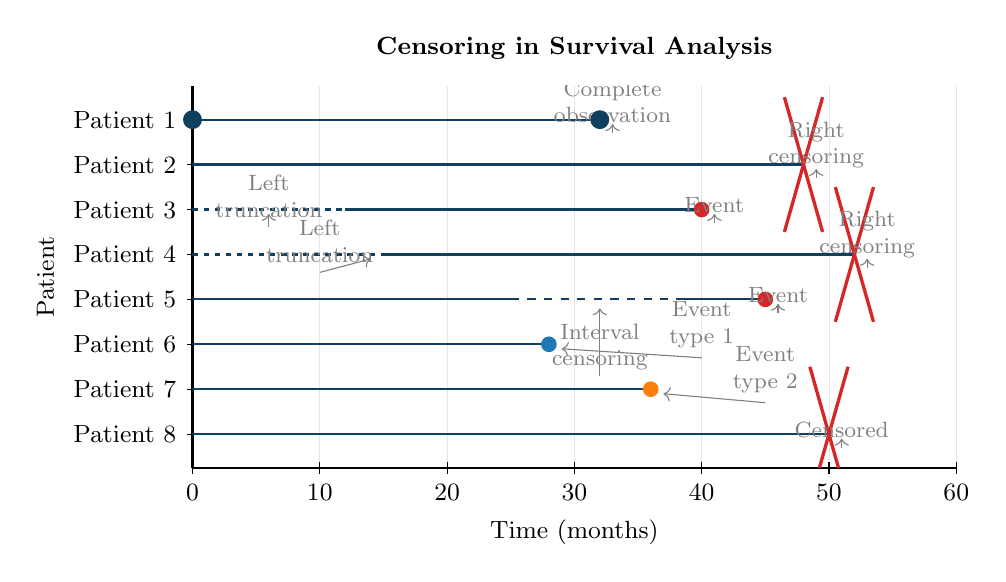
\begin{tikzpicture}
        \begin{axis}[
            publication,
            width=0.8\textwidth,
            height=0.4\textwidth,
            title={Censoring in Survival Analysis},
            xlabel={Time (months)},
            ylabel={Patient},
            ytick={1,2,3,4,5,6,7,8},
            yticklabels={Patient 1, Patient 2, Patient 3, Patient 4, Patient 5, Patient 6, Patient 7, Patient 8},
            xmin=0,
            xmax=60,
            ymin=0.25,
            ymax=8.75,
            xmajorgrids=true,
            grid style={octonary!20, very thin},
            y dir=reverse,
            legend pos=north east,
            legend style={
                font=\small,
                cells={anchor=west}
            }
        ]
            % Full observation (event occurred)
            \addplot[
                primaryDark,
                thick,
                mark=*,
                mark size=3pt,
                mark options={fill=primaryDark, solid}
            ] coordinates {
                (0,1) (32,1)
            };
            
            % Add death mark
            \node[circle, fill=quaternary, inner sep=2pt] at (axis cs:32,1) {};
            
            % Right-censored observation
            \addplot[
                primaryDark,
                thick,
                mark=none
            ] coordinates {
                (0,2) (48,2)
            };
            
            % Add censoring mark
            \draw[censoringColor, very thick] 
                (axis cs:48-1.5,2-1.5) -- (axis cs:48+1.5,2+1.5);
            \draw[censoringColor, very thick] 
                (axis cs:48-1.5,2+1.5) -- (axis cs:48+1.5,2-1.5);
                
            % Late entry (left truncation)
            \addplot[
                primaryDark,
                thick,
                mark=none,
                dash pattern=on 2pt off 2pt
            ] coordinates {
                (0,3) (12,3)
            };
            
            \addplot[
                primaryDark,
                thick,
                mark=none
            ] coordinates {
                (12,3) (40,3)
            };
            
            % Add death mark
            \node[circle, fill=quaternary, inner sep=2pt] at (axis cs:40,3) {};
            
            % Left truncation and right censoring
            \addplot[
                primaryDark,
                thick,
                mark=none,
                dash pattern=on 2pt off 2pt
            ] coordinates {
                (0,4) (15,4)
            };
            
            \addplot[
                primaryDark,
                thick,
                mark=none
            ] coordinates {
                (15,4) (52,4)
            };
            
            % Add censoring mark
            \draw[censoringColor, very thick] 
                (axis cs:52-1.5,4-1.5) -- (axis cs:52+1.5,4+1.5);
            \draw[censoringColor, very thick] 
                (axis cs:52-1.5,4+1.5) -- (axis cs:52+1.5,4-1.5);
                
            % Interval censoring
            \addplot[
                primaryDark,
                thick,
                mark=none
            ] coordinates {
                (0,5) (25,5)
            };
            
            \addplot[
                primaryDark,
                thick,
                mark=none,
                dash pattern=on 3pt off 3pt
            ] coordinates {
                (25,5) (38,5)
            };
            
            \addplot[
                primaryDark,
                thick,
                mark=none
            ] coordinates {
                (38,5) (45,5)
            };
            
            % Add death mark
            \node[circle, fill=quaternary, inner sep=2pt] at (axis cs:45,5) {};
            
            % Add interval censoring annotation arrow - moved up to avoid overlap with Event type 1
            \draw[->, thin, gray] (32,6.7) -- (32,5.2);
            \node[above, align=center, font=\footnotesize, text=gray] at (32,6.8) {Interval\\censoring};
            
            % Event observed in competing risks
            \addplot[
                primaryDark,
                thick,
                mark=none
            ] coordinates {
                (0,6) (28,6)
            };
            
            % Event 1 mark
            \node[circle, fill=event1Color, inner sep=2pt] at (axis cs:28,6) {};
            
            % Another competing risk event
            \addplot[
                primaryDark,
                thick,
                mark=none
            ] coordinates {
                (0,7) (36,7)
            };
            
            % Event 2 mark
            \node[circle, fill=event2Color, inner sep=2pt] at (axis cs:36,7) {};
            
            % Another competing risk with censoring
            \addplot[
                primaryDark,
                thick,
                mark=none
            ] coordinates {
                (0,8) (50,8)
            };
            
            % Censoring mark
            \draw[censoringColor, very thick] 
                (axis cs:50-1.5,8-1.5) -- (axis cs:50+1.5,8+1.5);
            \draw[censoringColor, very thick] 
                (axis cs:50-1.5,8+1.5) -- (axis cs:50+1.5,8-1.5);
            
            % Add labels with arrows to explain censoring concepts clearly
            % Complete observation
            \draw[->, thin, gray] (33,1.3) -- (33,1.1);
            \node[above, align=center, font=\footnotesize, text=gray] at (33,1.3) {Complete\\observation};
            
            % Right censoring
            \draw[->, thin, gray] (49,2.3) -- (49,2.1);
            \node[above, align=center, font=\footnotesize, text=gray] at (49,2.3) {Right\\censoring};
            
            % Left truncation (Patient 3)
            \draw[->, thin, gray] (6,3.4) -- (6,3.1);
            \node[above, align=center, font=\footnotesize, text=gray] at (6,3.4) {Left\\truncation};
            
            % Event mark
            \draw[->, thin, gray] (41,3.3) -- (41,3.1);
            \node[above, align=center, font=\footnotesize, text=gray] at (41,3.3) {Event};
            
            % Left truncation (Patient 4)
            \draw[->, thin, gray] (10,4.4) -- (14,4.1);
            \node[above, align=center, font=\footnotesize, text=gray] at (10,4.4) {Left\\truncation};
            
            % Right censoring (Patient 4)
            \draw[->, thin, gray] (53,4.3) -- (53,4.1);
            \node[above, align=center, font=\footnotesize, text=gray] at (53,4.3) {Right\\censoring};
            
            % Event after interval
            \draw[->, thin, gray] (46,5.3) -- (46,5.1);
            \node[above, align=center, font=\footnotesize, text=gray] at (46,5.3) {Event};
            
            % Event type 1 - shifted to the right where there's more space
            \draw[->, thin, gray] (40,6.3) -- (29,6.1);
            \node[above, align=center, font=\footnotesize, text=gray] at (40,6.3) {Event\\type 1};
            
            % Event type 2 - shifted to the right where there's more space
            \draw[->, thin, gray] (45,7.3) -- (37,7.1);
            \node[above, align=center, font=\footnotesize, text=gray] at (45,7.3) {Event\\type 2};
            
            % Censored
            \draw[->, thin, gray] (51,8.3) -- (51,8.1);
            \node[above, align=center, font=\footnotesize, text=gray] at (51,8.3) {Censored};
            
            % Add a legend at the bottom of the plot instead of top-right
            \legend{}
            
            % Create a separate legend below the plot using nodes
            \coordinate (legendpos) at (rel axis cs:0.5,-0.25);
            
            % Symbol for event of interest
            \node[inner sep=0] at ($(legendpos)+(-4.5,0)$) {\tikz{\draw[mark size=3pt, mark=*, mark options={fill=quaternary}] plot coordinates {(0,0)};}};
            \node[right, font=\footnotesize] at ($(legendpos)+(-4.3,0)$) {Event of interest};
            
            % Symbol for competing event type 1
            \node[inner sep=0] at ($(legendpos)+(-1.5,0)$) {\tikz{\draw[mark size=3pt, mark=*, mark options={fill=event1Color}] plot coordinates {(0,0)};}};
            \node[right, font=\footnotesize] at ($(legendpos)+(-1.3,0)$) {Competing event type 1};
            
            % Symbol for competing event type 2
            \node[inner sep=0] at ($(legendpos)+(1.5,0)$) {\tikz{\draw[mark size=3pt, mark=*, mark options={fill=event2Color}] plot coordinates {(0,0)};}};
            \node[right, font=\footnotesize] at ($(legendpos)+(1.7,0)$) {Competing event type 2};
            
            % Symbol for censoring
            \node[inner sep=0] at ($(legendpos)+(-4.5,-0.5)$) {\tikz{\draw[censoringColor, very thick] (-0.1,-0.1) -- (0.1,0.1); \draw[censoringColor, very thick] (-0.1,0.1) -- (0.1,-0.1);}};
            \node[right, font=\footnotesize] at ($(legendpos)+(-4.3,-0.5)$) {Censoring};
            
            % Symbol for observation time
            \node[inner sep=0] at ($(legendpos)+(-1.5,-0.5)$) {\tikz{\draw[primaryDark, thick] (-0.15,0) -- (0.15,0);}};
            \node[right, font=\footnotesize] at ($(legendpos)+(-1.3,-0.5)$) {Observation time};
            
            % Symbol for unobserved time
            \node[inner sep=0] at ($(legendpos)+(1.5,-0.5)$) {\tikz{\draw[primaryDark, thick, dash pattern=on 2pt off 2pt] (-0.15,0) -- (0.15,0);}};
            \node[right, font=\footnotesize] at ($(legendpos)+(1.7,-0.5)$) {Unobserved time};
        \end{axis}
    \end{tikzpicture}
    \caption{Different types of censoring in survival analysis and competing risks. The plot shows various scenarios including complete observation, right censoring, left truncation, interval censoring, and competing risks. Solid lines represent observed follow-up, dashed lines represent unobserved time, and markers indicate events or censoring.}
    \label{fig:censoring}
\end{figure}

% Alternative version with focus on competing risks
\begin{figure}[htbp]
    \centering
    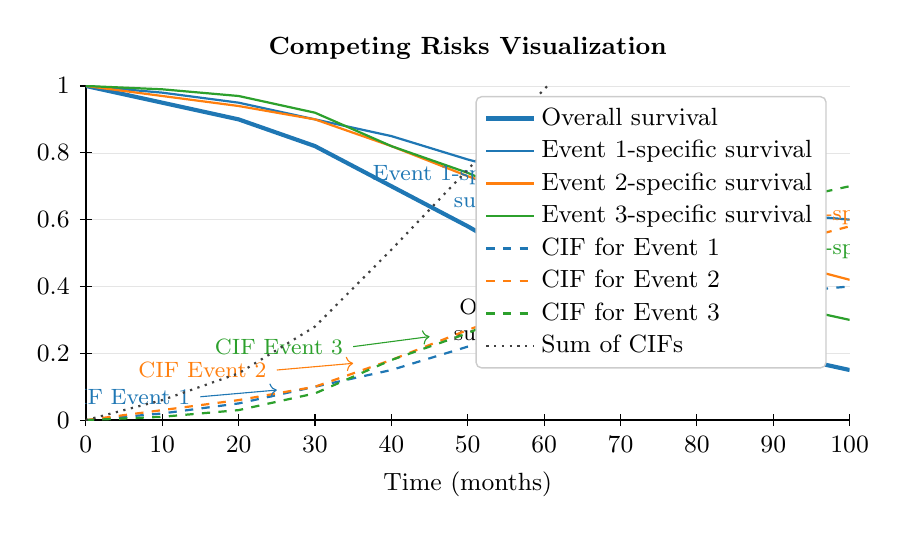
\begin{tikzpicture}
        \begin{axis}[
            publication,
            width=0.8\textwidth,
            height=0.35\textwidth,
            title={Competing Risks Visualization},
            xlabel={Time (months)},
            ylabel={},
            xmin=0,
            xmax=100,
            ymin=0,
            ymax=1,
            ymajorgrids=true,
            grid style={octonary!20, very thin},
            legend pos=north east,
            legend style={
                font=\small,
                cells={anchor=west}
            }
        ]
            % Overall Survival
            \addplot[
                survivalFunctionColor,
                custom ultra thick,
            ] coordinates {
                (0,1) (10,0.95) (20,0.9) (30,0.82) (40,0.7)
                (50,0.58) (60,0.45) (70,0.35) (80,0.27) (90,0.2) (100,0.15)
            };
            
            % Cause-specific survival curves
            \addplot[
                event1Color,
                thick,
            ] coordinates {
                (0,1) (10,0.98) (20,0.95) (30,0.9) (40,0.85)
                (50,0.78) (60,0.72) (70,0.68) (80,0.65) (90,0.62) (100,0.6)
            };
            
            \addplot[
                event2Color,
                thick,
            ] coordinates {
                (0,1) (10,0.97) (20,0.94) (30,0.9) (40,0.82)
                (50,0.73) (60,0.65) (70,0.58) (80,0.53) (90,0.48) (100,0.42)
            };
            
            \addplot[
                event3Color,
                thick,
            ] coordinates {
                (0,1) (10,0.99) (20,0.97) (30,0.92) (40,0.82)
                (50,0.74) (60,0.64) (70,0.52) (80,0.43) (90,0.35) (100,0.30)
            };
            
            % Add annotations with arrows for better readability
            \draw[->, thin] (60,0.3) -- (65,0.35);
            \node[left, align=right, font=\footnotesize] at (60,0.3) {Overall\\survival};
            
            \draw[->, thin, event1Color] (60,0.7) -- (65,0.68);
            \node[left, align=right, font=\footnotesize, text=event1Color] at (60,0.7) {Event 1-specific\\survival};
            
            \draw[->, thin, event2Color] (85,0.58) -- (80,0.58);
            \node[right, align=left, font=\footnotesize, text=event2Color] at (85,0.58) {Event 2-specific\\survival};
            
            \draw[->, thin, event3Color] (85,0.48) -- (80,0.48);
            \node[right, align=left, font=\footnotesize, text=event3Color] at (85,0.48) {Event 3-specific\\survival};
            
            % Cumulative incidence curves
            \addplot[
                event1Color,
                dashed,
                thick,
            ] coordinates {
                (0,0) (10,0.02) (20,0.05) (30,0.10) (40,0.15)
                (50,0.22) (60,0.28) (70,0.32) (80,0.35) (90,0.38) (100,0.40)
            };
            
            \addplot[
                event2Color,
                dashed,
                thick,
            ] coordinates {
                (0,0) (10,0.03) (20,0.06) (30,0.1) (40,0.18)
                (50,0.27) (60,0.35) (70,0.42) (80,0.47) (90,0.52) (100,0.58)
            };
            
            \addplot[
                event3Color,
                dashed,
                thick,
            ] coordinates {
                (0,0) (10,0.01) (20,0.03) (30,0.08) (40,0.18)
                (50,0.26) (60,0.36) (70,0.48) (80,0.57) (90,0.65) (100,0.70)
            };
            
            % Add annotations for CIF with improved positioning and arrows
            \draw[->, thin, event1Color] (15,0.07) -- (25,0.09);
            \node[left, align=right, font=\footnotesize, text=event1Color] at (15,0.07) {CIF Event 1};
            
            \draw[->, thin, event2Color] (25,0.15) -- (35,0.17);
            \node[left, align=right, font=\footnotesize, text=event2Color] at (25,0.15) {CIF Event 2};
            
            \draw[->, thin, event3Color] (35,0.22) -- (45,0.25);
            \node[left, align=right, font=\footnotesize, text=event3Color] at (35,0.22) {CIF Event 3};
            
            % Stacked CIF curve showing all events
            \addplot[
                octonaryDark,
                dotted,
                thick,
            ] coordinates {
                (0,0) (10,0.06) (20,0.14) (30,0.28) (40,0.51)
                (50,0.75) (60,0.99) (70,1.22) (80,1.39) (90,1.55) (100,1.68)
            };
            
            % Legend
            \addlegendentry{Overall survival};
            \addlegendentry{Event 1-specific survival};
            \addlegendentry{Event 2-specific survival};
            \addlegendentry{Event 3-specific survival};
            \addlegendentry{CIF for Event 1};
            \addlegendentry{CIF for Event 2};
            \addlegendentry{CIF for Event 3};
            \addlegendentry{Sum of CIFs};
        \end{axis}
    \end{tikzpicture}
    \caption{Visualization of competing risks: survival curves and cumulative incidence functions (CIFs). The overall survival (thick blue line) decreases more rapidly than any cause-specific survival curve. The dashed lines show the cumulative incidence functions for each competing event. Note that the sum of all CIFs (dotted line) can exceed 1.0 when viewing causes independently, illustrating why proper competing risks analysis is important.}
    \label{fig:competing-risks}
\end{figure}

\begin{definitionbox}[title=Censoring Types]
Censoring occurs when the event time is not precisely observed but is known to occur within a certain time range. The three main types of censoring are:
\begin{itemize}
    \item \textbf{Right censoring:} The most common type, occurs when a subject has not experienced the event of interest by the end of the study, is lost to follow-up, or withdraws from the study. Right censoring gives us a lower bound on the true time-to-event.

    \item \textbf{Left censoring:} Occurs when the event is known to have occurred before the first observation time, but the exact time is unknown. We only know that $T < t_{first}$.

    \item \textbf{Interval censoring:} Occurs when we only know that the event occurred within a certain time interval, but not the exact time. This happens when subjects are assessed periodically, and the event is detected at a follow-up visit.
\end{itemize}
\end{definitionbox}

The Kaplan-Meier estimator and Cox proportional hazards model both handle right censoring. Left truncation can be accommodated by modifying the risk sets in these methods. Interval censoring requires specialized techniques like the Turnbull estimator or parametric models.

\subsection{Time-to-Event Data Visualization}
\label{subsec:time-to-event}

The following visualizations illustrate time-to-event data for individual subjects and specific examples of different censoring types:

% Time-to-event data visualization with five subjects
% Following the publication-grade style guide

\begin{figure}[htbp]
    \centering
    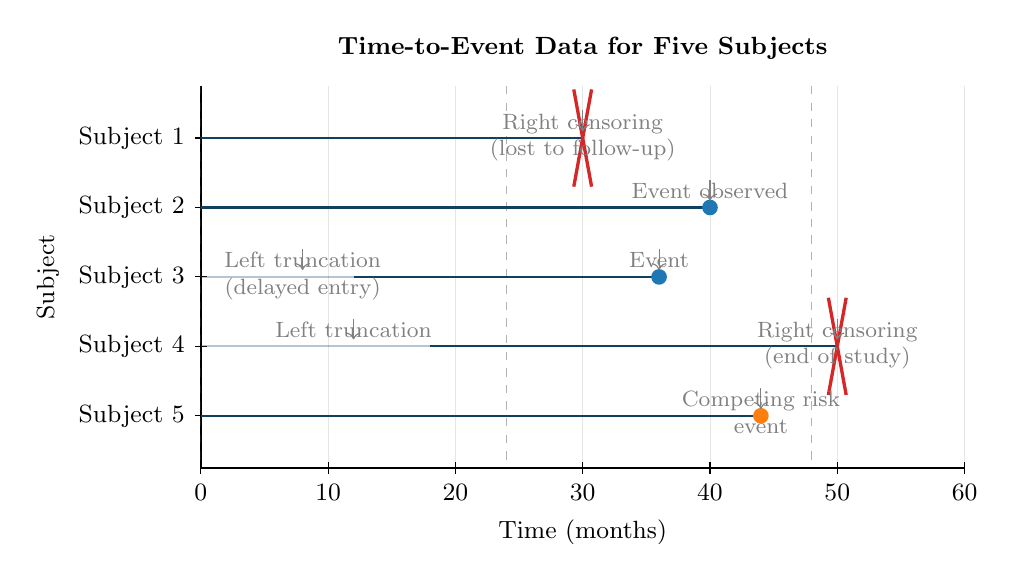
\begin{tikzpicture}
        \begin{axis}[
            publication,
            width=0.8\textwidth,
            height=0.4\textwidth,
            title={Time-to-Event Data for Five Subjects},
            xlabel={Time (months)},
            ylabel={Subject},
            ytick={1,2,3,4,5},
            yticklabels={Subject 1, Subject 2, Subject 3, Subject 4, Subject 5},
            xmin=0,
            xmax=60,
            ymin=0.25,
            ymax=5.75,
            xmajorgrids=true,
            grid style={octonary!20, very thin},
            y dir=reverse,
            legend pos=north east,
            legend style={
                font=\small,
                cells={anchor=west}
            }
        ]
            % Study timeline reference points
            \draw[thin, octonary!60, dashed] (0,0.25) -- (0,5.75);
            \draw[thin, octonary!60, dashed] (24,0.25) -- (24,5.75);
            \draw[thin, octonary!60, dashed] (48,0.25) -- (48,5.75);
            \node[below, font=\footnotesize, text=octonary] at (0,5.75) {Study start};
            \node[below, font=\footnotesize, text=octonary] at (24,5.75) {2 years};
            \node[below, font=\footnotesize, text=octonary] at (48,5.75) {4 years};
            
            % Subject 1: Standard right censoring
            \addplot[
                primaryDark,
                thick,
                mark=none
            ] coordinates {
                (0,1) (30,1)
            };
            
            % Add censoring mark
            \draw[censoringColor, very thick] 
                (30-0.7,1-0.7) -- (30+0.7,1+0.7);
            \draw[censoringColor, very thick] 
                (30-0.7,1+0.7) -- (30+0.7,1-0.7);
                
            % Subject 2: Event observed
            \addplot[
                primaryDark,
                thick,
                mark=none
            ] coordinates {
                (0,2) (40,2)
            };
            
            % Event mark
            \node[circle, fill=event1Color, inner sep=2pt] at (40,2) {};
            
            % Subject 3: Left truncation (delayed entry) + event
            \addplot[
                primaryDark,
                thick,
                mark=none,
                opacity=0.3
            ] coordinates {
                (0,3) (12,3)
            };
            
            \addplot[
                primaryDark,
                thick,
                mark=none
            ] coordinates {
                (12,3) (36,3)
            };
            
            % Event mark
            \node[circle, fill=event1Color, inner sep=2pt] at (36,3) {};
            
            % Subject 4: Left truncation + right censoring
            \addplot[
                primaryDark,
                thick,
                mark=none,
                opacity=0.3
            ] coordinates {
                (0,4) (18,4)
            };
            
            \addplot[
                primaryDark,
                thick,
                mark=none
            ] coordinates {
                (18,4) (50,4)
            };
            
            % Add censoring mark
            \draw[censoringColor, very thick] 
                (50-0.7,4-0.7) -- (50+0.7,4+0.7);
            \draw[censoringColor, very thick] 
                (50-0.7,4+0.7) -- (50+0.7,4-0.7);
                
            % Subject 5: Competing risk
            \addplot[
                primaryDark,
                thick,
                mark=none
            ] coordinates {
                (0,5) (44,5)
            };
            
            % Competing risk event mark
            \node[circle, fill=event2Color, inner sep=2pt] at (44,5) {};
            
            % Labels with arrows - positioned to avoid crossing lines
            % Subject 1: Right censoring
            \draw[->, thin, gray] (30,0.6) -- (30,0.9);
            \node[below, align=center, font=\footnotesize, text=gray] at (30,0.5) {Right censoring\\(lost to follow-up)};
            
            % Subject 2: Event
            \draw[->, thin, gray] (40,1.6) -- (40,1.9);
            \node[below, align=center, font=\footnotesize, text=gray] at (40,1.5) {Event observed};
            
            % Subject 3: Left truncation
            \draw[->, thin, gray] (8,2.6) -- (8,2.9);
            \node[below, align=center, font=\footnotesize, text=gray] at (8,2.5) {Left truncation\\(delayed entry)};
            
            % Subject 3: Event
            \draw[->, thin, gray] (36,2.6) -- (36,2.9);
            \node[below, align=center, font=\footnotesize, text=gray] at (36,2.5) {Event};
            
            % Subject 4: Left truncation
            \draw[->, thin, gray] (12,3.6) -- (12,3.9);
            \node[below, align=center, font=\footnotesize, text=gray] at (12,3.5) {Left truncation};
            
            % Subject 4: Right censoring
            \draw[->, thin, gray] (50,3.6) -- (50,3.9);
            \node[below, align=center, font=\footnotesize, text=gray] at (50,3.5) {Right censoring\\(end of study)};
            
            % Subject 5: Competing risk
            \draw[->, thin, gray] (44,4.6) -- (44,4.9);
            \node[below, align=center, font=\footnotesize, text=gray] at (44,4.5) {Competing risk\\event};
            
            % Add a legend at the bottom of the plot instead of top-right
            \legend{}
            
            % Create a separate legend below the plot using nodes
            \coordinate (legendpos) at (rel axis cs:0.5,-0.25);
            
            % Symbol for observation time
            \node[inner sep=0] at ($(legendpos)+(-4.5,0)$) {\tikz{\draw[primaryDark, thick] (-0.15,0) -- (0.15,0);}};
            \node[right, font=\footnotesize] at ($(legendpos)+(-4.3,0)$) {Observation time};
            
            % Symbol for unobserved time
            \node[inner sep=0] at ($(legendpos)+(-1.5,0)$) {\tikz{\draw[primaryDark, thick, opacity=0.3] (-0.15,0) -- (0.15,0);}};
            \node[right, font=\footnotesize] at ($(legendpos)+(-1.3,0)$) {Unobserved time};
            
            % Symbol for event of interest
            \node[inner sep=0] at ($(legendpos)+(1.5,0)$) {\tikz{\draw[mark size=3pt, mark=*, mark options={fill=event1Color}] plot coordinates {(0,0)};}};
            \node[right, font=\footnotesize] at ($(legendpos)+(1.7,0)$) {Event of interest};
            
            % Symbol for competing event
            \node[inner sep=0] at ($(legendpos)+(-4.5,-0.5)$) {\tikz{\draw[mark size=3pt, mark=*, mark options={fill=event2Color}] plot coordinates {(0,0)};}};
            \node[right, font=\footnotesize] at ($(legendpos)+(-4.3,-0.5)$) {Competing event};
            
            % Symbol for censoring
            \node[inner sep=0] at ($(legendpos)+(-1.5,-0.5)$) {\tikz{\draw[censoringColor, very thick] (-0.1,-0.1) -- (0.1,0.1); \draw[censoringColor, very thick] (-0.1,0.1) -- (0.1,-0.1);}};
            \node[right, font=\footnotesize] at ($(legendpos)+(-1.3,-0.5)$) {Censoring};
        \end{axis}
    \end{tikzpicture}
    \caption{Time-to-event data for five subjects showing various censoring and event patterns. Subject 1 experiences right censoring due to loss to follow-up. Subject 2 has an observed event. Subject 3 enters the study late (left truncation) and experiences an event. Subject 4 enters late and is right-censored at the end of the study. Subject 5 experiences a competing risk event.}
    \label{fig:time-to-event-subjects}
\end{figure}

% Visualization of left censoring examples
\begin{figure}[htbp]
    \centering
    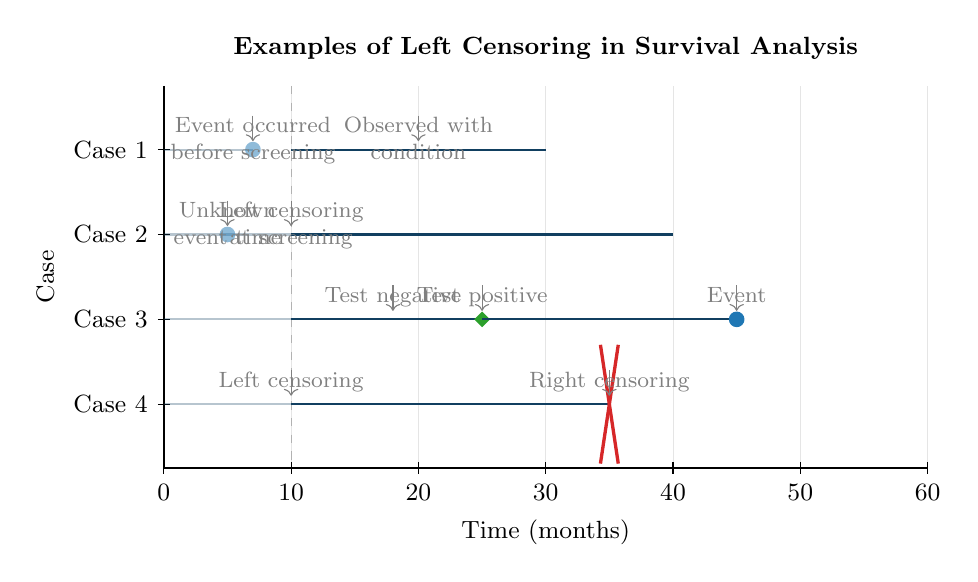
\begin{tikzpicture}
        \begin{axis}[
            publication,
            width=0.8\textwidth,
            height=0.4\textwidth,
            title={Examples of Left Censoring in Survival Analysis},
            xlabel={Time (months)},
            ylabel={Case},
            ytick={1,2,3,4},
            yticklabels={Case 1, Case 2, Case 3, Case 4},
            xmin=0,
            xmax=60,
            ymin=0.25,
            ymax=4.75,
            xmajorgrids=true,
            grid style={octonary!20, very thin},
            y dir=reverse,
            legend pos=north east,
            legend style={
                font=\small,
                cells={anchor=west}
            }
        ]
            % Timeline reference points
            \draw[thin, octonary!60, dashed] (10,0.25) -- (10,4.75);
            \node[below, font=\footnotesize, text=octonary] at (10,4.75) {Screening time};
            
            % Case 1: Event known to occur before screening
            % Unobserved event time
            \addplot[
                primaryDark,
                thick,
                mark=none,
                opacity=0.3
            ] coordinates {
                (0,1) (7,1)
            };
            
            % Event mark (not directly observed)
            \node[circle, fill=event1Color, inner sep=2pt, opacity=0.5] at (7,1) {};
            
            % Observed after event
            \addplot[
                primaryDark,
                thick,
                mark=none
            ] coordinates {
                (10,1) (30,1)
            };
            
            % Case 2: Condition present at screening
            % Unobserved event time
            \addplot[
                primaryDark,
                thick,
                mark=none,
                opacity=0.3
            ] coordinates {
                (0,2) (10,2)
            };
            
            % Event before screening
            \node[circle, fill=event1Color, inner sep=2pt, opacity=0.5] at (5,2) {};
            
            % Left censoring mark at screening
            \draw[censoringColor, very thick, rotate=180] 
                (10-0.7,2-0.7) -- (10+0.7,2+0.7);
            \draw[censoringColor, very thick, rotate=180] 
                (10-0.7,2+0.7) -- (10+0.7,2-0.7);
                
            % Observed after positive screening
            \addplot[
                primaryDark,
                thick,
                mark=none
            ] coordinates {
                (10,2) (40,2)
            };
            
            % Case 3: Test detects condition with delay, then event
            % Unobserved period
            \addplot[
                primaryDark,
                thick,
                mark=none,
                opacity=0.3
            ] coordinates {
                (0,3) (10,3)
            };
            
            % Tested negative at first
            \addplot[
                primaryDark,
                thick,
                mark=none
            ] coordinates {
                (10,3) (25,3)
            };
            
            % Test detects condition
            \node[diamond, fill=event3Color, inner sep=1.5pt] at (25,3) {};
            
            % Followed until event
            \addplot[
                primaryDark,
                thick,
                mark=none
            ] coordinates {
                (25,3) (45,3)
            };
            
            % Event mark
            \node[circle, fill=event1Color, inner sep=2pt] at (45,3) {};
            
            % Case 4: Left and right censoring
            % Left censored unobserved period
            \addplot[
                primaryDark,
                thick,
                mark=none,
                opacity=0.3
            ] coordinates {
                (0,4) (10,4)
            };
            
            % Left censoring mark
            \draw[censoringColor, very thick, rotate=180] 
                (10-0.7,4-0.7) -- (10+0.7,4+0.7);
            \draw[censoringColor, very thick, rotate=180] 
                (10-0.7,4+0.7) -- (10+0.7,4-0.7);
                
            % Observed period
            \addplot[
                primaryDark,
                thick,
                mark=none
            ] coordinates {
                (10,4) (35,4)
            };
            
            % Right censoring mark
            \draw[censoringColor, very thick] 
                (35-0.7,4-0.7) -- (35+0.7,4+0.7);
            \draw[censoringColor, very thick] 
                (35-0.7,4+0.7) -- (35+0.7,4-0.7);
                
            % Labels with arrows - positioned to avoid crossing lines
            % Case 1
            \draw[->, thin, gray] (7,0.6) -- (7,0.9);
            \node[below, align=center, font=\footnotesize, text=gray] at (7,0.5) {Event occurred\\before screening};
            
            \draw[->, thin, gray] (20,0.6) -- (20,0.9);
            \node[below, align=center, font=\footnotesize, text=gray] at (20,0.5) {Observed with\\condition};
            
            % Case 2
            \draw[->, thin, gray] (5,1.6) -- (5,1.9);
            \node[below, align=center, font=\footnotesize, text=gray] at (5,1.5) {Unknown\\event time};
            
            \draw[->, thin, gray] (10,1.6) -- (10,1.9);
            \node[below, align=center, font=\footnotesize, text=gray] at (10,1.5) {Left censoring\\at screening};
            
            % Case 3
            \draw[->, thin, gray] (18,2.6) -- (18,2.9);
            \node[below, align=center, font=\footnotesize, text=gray] at (18,2.5) {Test negative};
            
            \draw[->, thin, gray] (25,2.6) -- (25,2.9);
            \node[below, align=center, font=\footnotesize, text=gray] at (25,2.5) {Test positive};
            
            \draw[->, thin, gray] (45,2.6) -- (45,2.9);
            \node[below, align=center, font=\footnotesize, text=gray] at (45,2.5) {Event};
            
            % Case 4
            \draw[->, thin, gray] (10,3.6) -- (10,3.9);
            \node[below, align=center, font=\footnotesize, text=gray] at (10,3.5) {Left censoring};
            
            \draw[->, thin, gray] (35,3.6) -- (35,3.9);
            \node[below, align=center, font=\footnotesize, text=gray] at (35,3.5) {Right censoring};
            
            % Add a legend at the bottom of the plot instead of top-right
            \legend{}
            
            % Create a separate legend below the plot using nodes
            \coordinate (legendpos) at (rel axis cs:0.5,-0.3);
            
            % Row 1
            % Symbol for observed follow-up
            \node[inner sep=0] at ($(legendpos)+(-4.5,0.3)$) {\tikz{\draw[primaryDark, thick] (-0.15,0) -- (0.15,0);}};
            \node[right, font=\footnotesize] at ($(legendpos)+(-4.3,0.3)$) {Observed follow-up};
            
            % Symbol for unobserved time
            \node[inner sep=0] at ($(legendpos)+(-1.5,0.3)$) {\tikz{\draw[primaryDark, thick, opacity=0.3] (-0.15,0) -- (0.15,0);}};
            \node[right, font=\footnotesize] at ($(legendpos)+(-1.3,0.3)$) {Unobserved time};
            
            % Symbol for observed event
            \node[inner sep=0] at ($(legendpos)+(1.5,0.3)$) {\tikz{\draw[mark size=3pt, mark=*, mark options={fill=event1Color}] plot coordinates {(0,0)};}};
            \node[right, font=\footnotesize] at ($(legendpos)+(1.7,0.3)$) {Observed event};
            
            % Row 2
            % Symbol for unobserved event
            \node[inner sep=0] at ($(legendpos)+(-4.5,0)$) {\tikz{\draw[mark size=3pt, mark=*, mark options={fill=event1Color, opacity=0.5}] plot coordinates {(0,0)};}};
            \node[right, font=\footnotesize] at ($(legendpos)+(-4.3,0)$) {Unobserved event};
            
            % Symbol for test detection
            \node[inner sep=0] at ($(legendpos)+(-1.5,0)$) {\tikz{\draw[mark size=3pt, mark=diamond, mark options={fill=event3Color}] plot coordinates {(0,0)};}};
            \node[right, font=\footnotesize] at ($(legendpos)+(-1.3,0)$) {Test detection};
            
            % Row 3
            % Symbol for right censoring
            \node[inner sep=0] at ($(legendpos)+(-4.5,-0.3)$) {\tikz{\draw[censoringColor, very thick] (-0.1,-0.1) -- (0.1,0.1); \draw[censoringColor, very thick] (-0.1,0.1) -- (0.1,-0.1);}};
            \node[right, font=\footnotesize] at ($(legendpos)+(-4.3,-0.3)$) {Right censoring};
            
            % Symbol for left censoring
            \node[inner sep=0] at ($(legendpos)+(-1.5,-0.3)$) {\tikz{\draw[censoringColor, very thick, rotate=180] (-0.1,-0.1) -- (0.1,0.1); \draw[censoringColor, very thick, rotate=180] (-0.1,0.1) -- (0.1,-0.1);}};
            \node[right, font=\footnotesize] at ($(legendpos)+(-1.3,-0.3)$) {Left censoring};
        \end{axis}
    \end{tikzpicture}
    \caption{Examples of left censoring in survival analysis. Case 1 shows an event known to have occurred before screening, with the exact time unknown. Case 2 shows a condition detected at the initial screening (left censored). Case 3 shows delayed detection where a test initially misses the condition but later detects it. Case 4 shows both left and right censoring in the same subject. For left censoring, we only know that the event occurred before a certain time point, in contrast to right censoring where we know it occurred after.}
    \label{fig:left-censoring-examples}
\end{figure}

\subsection{Clinical Study Visualization}
\label{subsec:clinical-censoring}

The following visualization illustrates real-world patient follow-up patterns in a clinical trial setting:

% Clinical Study Censoring Visualization using our publication-grade styles
% This visualization shows patient follow-up in a longitudinal clinical study

\begin{figure}[htbp]
    \centering
    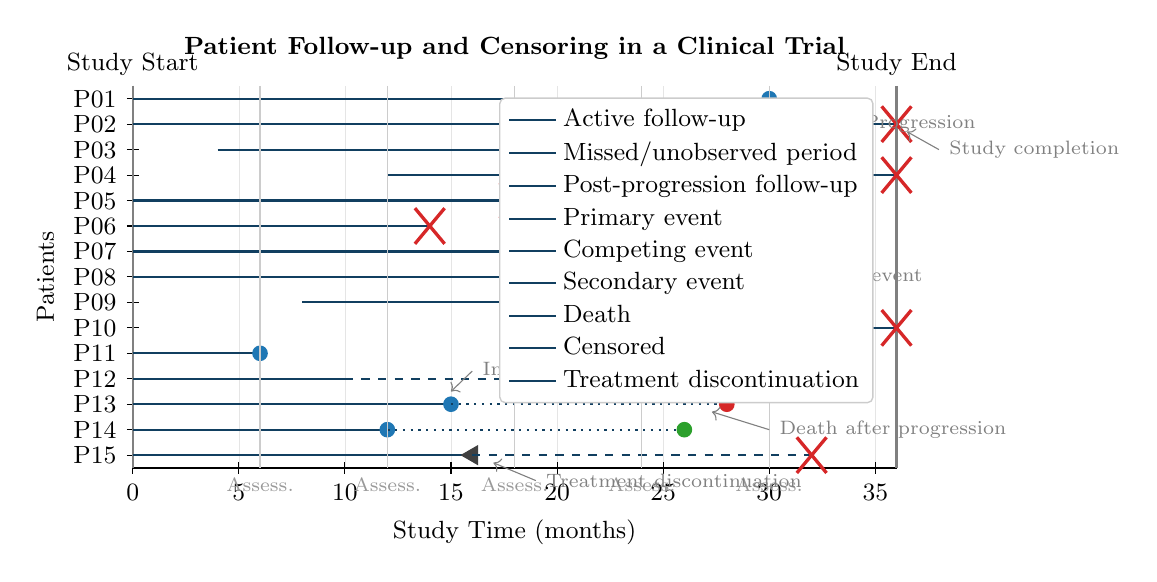
\begin{tikzpicture}
        \begin{axis}[
            publication,
            width=0.8\textwidth,
            height=0.4\textwidth,
            title={Patient Follow-up and Censoring in a Clinical Trial},
            xlabel={Study Time (months)},
            ylabel={Patients},
            ytick={1,2,3,4,5,6,7,8,9,10,11,12,13,14,15},
            yticklabels={P01, P02, P03, P04, P05, P06, P07, P08, P09, P10, P11, P12, P13, P14, P15},
            xmin=0,
            xmax=36,
            ymin=0.5,
            ymax=15.5,
            xmajorgrids=true,
            grid style={octonary!20, very thin},
            y dir=reverse,
            legend pos=north east,
            legend style={
                font=\small,
                cells={anchor=west}
            },
            clip=false
        ]
            % Study timeline markers
            \draw[thick, gray] (0,0.5) -- (0,15.5);
            \draw[thick, gray] (36,0.5) -- (36,15.5);
            \node[above, font=\small] at (0,0.5) {Study Start};
            \node[above, font=\small] at (36,0.5) {Study End};

            % Patient 1: Complete follow-up, event at the end
            \addplot[
                primaryDark,
                thick,
                mark=none
            ] coordinates {
                (0,1) (30,1)
            };

            % Event mark (e.g., progression)
            \node[circle, fill=event1Color, inner sep=2pt] at (30,1) {};

            % Patient 2: Complete follow-up without event
            \addplot[
                primaryDark,
                thick,
                mark=none
            ] coordinates {
                (0,2) (36,2)
            };

            % Add censoring mark at study end
            \draw[censoringColor, very thick]
                (36-0.7,2-0.7) -- (36+0.7,2+0.7);
            \draw[censoringColor, very thick]
                (36-0.7,2+0.7) -- (36+0.7,2-0.7);

            % Patient 3: Early enrollment, event
            \addplot[
                primaryDark,
                thick,
                mark=none
            ] coordinates {
                (4,3) (22,3)
            };

            % Event mark
            \node[circle, fill=event1Color, inner sep=2pt] at (22,3) {};

            % Patient 4: Late enrollment, no event
            \addplot[
                primaryDark,
                thick,
                mark=none
            ] coordinates {
                (12,4) (36,4)
            };

            % Add censoring mark at study end
            \draw[censoringColor, very thick]
                (36-0.7,4-0.7) -- (36+0.7,4+0.7);
            \draw[censoringColor, very thick]
                (36-0.7,4+0.7) -- (36+0.7,4-0.7);

            % Patient 5: Lost to follow-up
            \addplot[
                primaryDark,
                thick,
                mark=none
            ] coordinates {
                (0,5) (18,5)
            };

            % Add censoring mark
            \draw[censoringColor, very thick]
                (18-0.7,5-0.7) -- (18+0.7,5+0.7);
            \draw[censoringColor, very thick]
                (18-0.7,5+0.7) -- (18+0.7,5-0.7);

            % Patient 6: Dropped out
            \addplot[
                primaryDark,
                thick,
                mark=none
            ] coordinates {
                (0,6) (14,6)
            };

            % Add censoring mark
            \draw[censoringColor, very thick]
                (14-0.7,6-0.7) -- (14+0.7,6+0.7);
            \draw[censoringColor, very thick]
                (14-0.7,6+0.7) -- (14+0.7,6-0.7);

            % Patient 7: Competing event (e.g., different progression type)
            \addplot[
                primaryDark,
                thick,
                mark=none
            ] coordinates {
                (0,7) (26,7)
            };

            % Competing event mark
            \node[circle, fill=event2Color, inner sep=2pt] at (26,7) {};

            % Patient 8: Death (as a separate event type)
            \addplot[
                primaryDark,
                thick,
                mark=none
            ] coordinates {
                (0,8) (20,8)
            };

            % Death mark
            \node[circle, fill=quaternary, inner sep=2pt] at (20,8) {};

            % Patient 9: Late enrollment, competing event
            \addplot[
                primaryDark,
                thick,
                mark=none
            ] coordinates {
                (8,9) (24,9)
            };

            % Competing event mark
            \node[circle, fill=event2Color, inner sep=2pt] at (24,9) {};

            % Patient 10: Very late enrollment, ongoing at study end
            \addplot[
                primaryDark,
                thick,
                mark=none
            ] coordinates {
                (28,10) (36,10)
            };

            % Add censoring mark at study end
            \draw[censoringColor, very thick]
                (36-0.7,10-0.7) -- (36+0.7,10+0.7);
            \draw[censoringColor, very thick]
                (36-0.7,10+0.7) -- (36+0.7,10-0.7);

            % Patient 11: Event very early
            \addplot[
                primaryDark,
                thick,
                mark=none
            ] coordinates {
                (0,11) (6,11)
            };

            % Event mark
            \node[circle, fill=event1Color, inner sep=2pt] at (6,11) {};

            % Patient 12: Interval censoring - missed visits, then event found
            \addplot[
                primaryDark,
                thick,
                mark=none
            ] coordinates {
                (0,12) (10,12)
            };

            % Missed follow-up
            \addplot[
                primaryDark,
                thick,
                dashed
            ] coordinates {
                (10,12) (20,12)
            };

            \addplot[
                primaryDark,
                thick,
                mark=none
            ] coordinates {
                (20,12) (20,12)
            };

            % Event mark
            \node[circle, fill=event1Color, inner sep=2pt] at (20,12) {};

            % Patient 13: Death after progression
            \addplot[
                primaryDark,
                thick,
                mark=none
            ] coordinates {
                (0,13) (15,13)
            };

            % Event mark (progression)
            \node[circle, fill=event1Color, inner sep=2pt] at (15,13) {};

            % Continue observation after progression
            \addplot[
                primaryDark,
                thick,
                dotted
            ] coordinates {
                (15,13) (28,13)
            };

            % Death mark
            \node[circle, fill=quaternary, inner sep=2pt] at (28,13) {};

            % Patient 14: Multiple events
            \addplot[
                primaryDark,
                thick,
                mark=none
            ] coordinates {
                (0,14) (12,14)
            };

            % First event
            \node[circle, fill=event1Color, inner sep=2pt] at (12,14) {};

            % Continue to second event
            \addplot[
                primaryDark,
                thick,
                dotted
            ] coordinates {
                (12,14) (26,14)
            };

            % Second event
            \node[circle, fill=event3Color, inner sep=2pt] at (26,14) {};

            % Patient 15: Treatment discontinuation
            \addplot[
                primaryDark,
                thick,
                mark=none
            ] coordinates {
                (0,15) (16,15)
            };

            % Treatment discontinuation mark (triangle)
            \node[regular polygon, regular polygon sides=3, fill=octonaryDark, inner sep=1.5pt, rotate=90] at (16,15) {};

            % Different line style after treatment
            \addplot[
                primaryDark,
                thick,
                dashed
            ] coordinates {
                (16,15) (32,15)
            };

            % Add censoring mark
            \draw[censoringColor, very thick]
                (32-0.7,15-0.7) -- (32+0.7,15+0.7);
            \draw[censoringColor, very thick]
                (32-0.7,15+0.7) -- (32+0.7,15-0.7);

            % Add colored vertical assessment period markers - avoiding \foreach
            \draw[octonary!40, thin] (6,0.5) -- (6,15.5);
            \draw[octonary!40, thin] (12,0.5) -- (12,15.5);
            \draw[octonary!40, thin] (18,0.5) -- (18,15.5);
            \draw[octonary!40, thin] (24,0.5) -- (24,15.5);
            \draw[octonary!40, thin] (30,0.5) -- (30,15.5);

            \node[below, font=\scriptsize, text=octonary!80] at (6,15.5) {Assess.};
            \node[below, font=\scriptsize, text=octonary!80] at (12,15.5) {Assess.};
            \node[below, font=\scriptsize, text=octonary!80] at (18,15.5) {Assess.};
            \node[below, font=\scriptsize, text=octonary!80] at (24,15.5) {Assess.};
            \node[below, font=\scriptsize, text=octonary!80] at (30,15.5) {Assess.};

            % Add annotations
            \draw[<-, gray, thin] (31,1.3) -- (34,2);
            \node[anchor=west, gray, font=\scriptsize] at (34,2) {Progression};

            \draw[<-, gray, thin] (36.5,2.3) -- (38,3);
            \node[anchor=west, gray, font=\scriptsize] at (38,3) {Study completion};

            \draw[<-, gray, thin] (19,5.3) -- (22,6);
            \node[anchor=west, gray, font=\scriptsize] at (22,6) {Lost to follow-up};

            \draw[<-, gray, thin] (26.5,7.3) -- (29,8);
            \node[anchor=west, gray, font=\scriptsize] at (29,8) {Competing event};

            \draw[<-, gray, thin] (20.5,8.3) -- (23,9);
            \node[anchor=west, gray, font=\scriptsize] at (23,9) {Death};

            \draw[<-, gray, thin] (15,12.5) -- (16,11.7);
            \node[anchor=west, gray, font=\scriptsize] at (16,11.7) {Interval censoring};

            \draw[<-, gray, thin] (27.3,13.3) -- (30,14);
            \node[anchor=west, gray, font=\scriptsize] at (30,14) {Death after progression};

            \draw[<-, gray, thin] (17,15.3) -- (19,16);
            \node[anchor=west, gray, font=\scriptsize] at (19,16) {Treatment discontinuation};

            % Legend entries
            \addlegendimage{primaryDark, thick}
            \addlegendentry{Active follow-up}

            \addlegendimage{primaryDark, thick, dashed}
            \addlegendentry{Missed/unobserved period}

            \addlegendimage{primaryDark, thick, dotted}
            \addlegendentry{Post-progression follow-up}

            \addlegendimage{mark=*, mark size=3pt, mark options={fill=event1Color, solid}, only marks}
            \addlegendentry{Primary event}

            \addlegendimage{mark=*, mark size=3pt, mark options={fill=event2Color, solid}, only marks}
            \addlegendentry{Competing event}

            \addlegendimage{mark=*, mark size=3pt, mark options={fill=event3Color, solid}, only marks}
            \addlegendentry{Secondary event}

            \addlegendimage{mark=*, mark size=3pt, mark options={fill=quaternary, solid}, only marks}
            \addlegendentry{Death}

            \addlegendimage{censoringColor, thick, mark=+, mark size=3pt}
            \addlegendentry{Censored}

            \addlegendimage{regular polygon, regular polygon sides=3, fill=octonaryDark, inner sep=1.5pt}
            \addlegendentry{Treatment discontinuation}
        \end{axis}
    \end{tikzpicture}
    \caption{Visualization of patient follow-up in a 36-month clinical trial. The plot shows various scenarios including complete follow-up, early/late enrollment, loss to follow-up, treatment discontinuation, competing events, and interval censoring. Vertical lines represent scheduled assessment visits at 6-month intervals. This visual representation illustrates the complexity of longitudinal data in clinical studies and the various types of censoring that must be accounted for in survival analysis.}
    \label{fig:clinical-censoring}
\end{figure}

% Time-to-event analysis visualization
\begin{figure}[htbp]
    \centering
    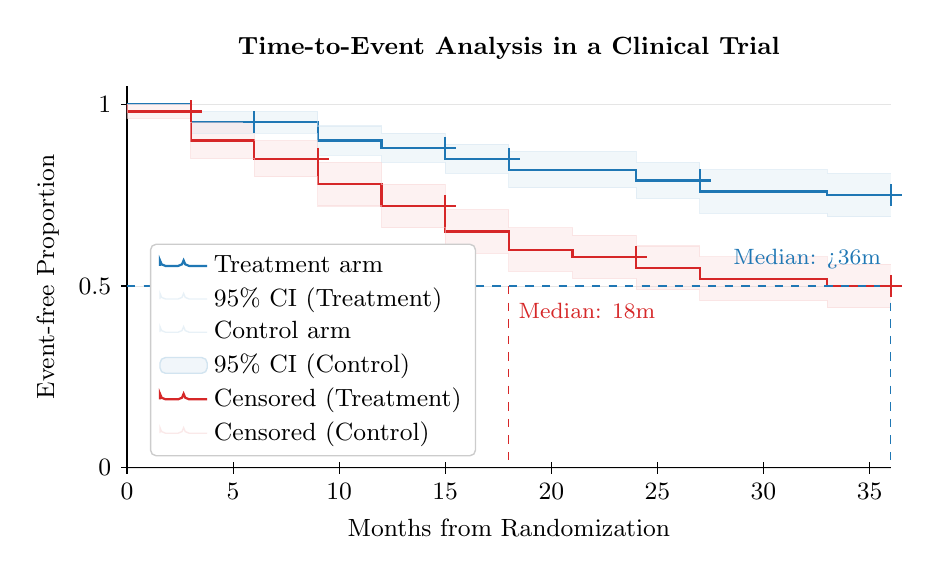
\begin{tikzpicture}
        \begin{axis}[
            publication,
            width=0.8\textwidth,
            height=0.4\textwidth,
            title={Time-to-Event Analysis in a Clinical Trial},
            xlabel={Months from Randomization},
            ylabel={Event-free Proportion},
            xmin=0,
            xmax=36,
            ymin=0,
            ymax=1.05,
            ymajorgrids=true,
            grid style={octonary!20, very thin},
            legend pos=south west,
            legend style={
                font=\small,
                cells={anchor=west}
            }
        ]
            % Kaplan-Meier Curve for Treatment Group
            \addplot[
                survivalFunctionColor,
                thick,
                const plot mark right,
                mark=none
            ] coordinates {
                (0, 1.0) (3, 1.0) (6, 0.95) (9, 0.95) (12, 0.90)
                (15, 0.88) (18, 0.85) (21, 0.82) (24, 0.82)
                (27, 0.79) (30, 0.76) (33, 0.76) (36, 0.75)
            };

            % Add confidence bands for treatment group
            \addplot[
                survivalFunctionColor!20,
                opacity=0.5,
                const plot mark right,
                mark=none,
                name path=upperT
            ] coordinates {
                (0, 1.0) (3, 1.0) (6, 0.98) (9, 0.98) (12, 0.94)
                (15, 0.92) (18, 0.89) (21, 0.87) (24, 0.87)
                (27, 0.84) (30, 0.82) (33, 0.82) (36, 0.81)
            };

            \addplot[
                survivalFunctionColor!20,
                opacity=0.5,
                const plot mark right,
                mark=none,
                name path=lowerT
            ] coordinates {
                (0, 1.0) (3, 1.0) (6, 0.92) (9, 0.92) (12, 0.86)
                (15, 0.84) (18, 0.81) (21, 0.77) (24, 0.77)
                (27, 0.74) (30, 0.70) (33, 0.70) (36, 0.69)
            };

            % Fill between confidence bands
            \addplot[
                survivalFunctionColor!20,
                fill opacity=0.3
            ] fill between[of=upperT and lowerT];

            % Kaplan-Meier Curve for Control Group
            \addplot[
                quaternary,
                thick,
                const plot mark right,
                mark=none
            ] coordinates {
                (0, 1.0) (3, 0.98) (6, 0.90) (9, 0.85) (12, 0.78)
                (15, 0.72) (18, 0.65) (21, 0.60) (24, 0.58)
                (27, 0.55) (30, 0.52) (33, 0.52) (36, 0.50)
            };

            % Add confidence bands for control group
            \addplot[
                quaternary!20,
                opacity=0.5,
                const plot mark right,
                mark=none,
                name path=upperC
            ] coordinates {
                (0, 1.0) (3, 1.0) (6, 0.95) (9, 0.90) (12, 0.84)
                (15, 0.78) (18, 0.71) (21, 0.66) (24, 0.64)
                (27, 0.61) (30, 0.58) (33, 0.58) (36, 0.56)
            };

            \addplot[
                quaternary!20,
                opacity=0.5,
                const plot mark right,
                mark=none,
                name path=lowerC
            ] coordinates {
                (0, 1.0) (3, 0.96) (6, 0.85) (9, 0.80) (12, 0.72)
                (15, 0.66) (18, 0.59) (21, 0.54) (24, 0.52)
                (27, 0.49) (30, 0.46) (33, 0.46) (36, 0.44)
            };

            % Fill between confidence bands
            \addplot[
                quaternary!20,
                fill opacity=0.3
            ] fill between[of=upperC and lowerC];

            % Add censoring marks
            % Treatment group
            \addplot[
                only marks,
                mark=+,
                mark size=4pt,
                mark options={solid, survivalFunctionColor}
            ] coordinates {
                (6, 0.95) (15, 0.88) (18, 0.85) (27, 0.79) (36, 0.75)
            };

            % Control group
            \addplot[
                only marks,
                mark=+,
                mark size=4pt,
                mark options={solid, quaternary}
            ] coordinates {
                (3, 0.98) (9, 0.85) (15, 0.72) (24, 0.58) (36, 0.50)
            };

            % Add simplified risk table
            \node[anchor=north west, align=left, font=\footnotesize] at (0,-0.12) {
                \begin{tabular}{@{}l@{\hspace{1pt}}|@{\hspace{1pt}}c@{\hspace{1pt}}c@{\hspace{1pt}}c@{\hspace{1pt}}c@{\hspace{1pt}}c@{\hspace{1pt}}c@{\hspace{1pt}}c@{}}
                \textbf{At risk} & \textbf{0} & \textbf{6} & \textbf{12} & \textbf{18} & \textbf{24} & \textbf{30} & \textbf{36} \\
                \hline
                Treat & 100 & 95 & 90 & 85 & 82 & 76 & 75 \\
                Ctrl & 100 & 90 & 78 & 65 & 58 & 52 & 50 \\
                \end{tabular}
            };

            % Add p-value and hazard ratio (simplified)
            \node[anchor=south east, align=right, font=\footnotesize] at (36,1.02) {
                \begin{tabular}{r}
                HR: 0.57 (0.41-0.78) \\
                $p = 0.0015$
                \end{tabular}
            };

            % Label median survival times
            \draw[dashed, quaternary] (0,0.5) -- (36,0.5);
            \draw[dashed, quaternary] (18,0.5) -- (18,0);
            \node[anchor=north west, font=\footnotesize, text=quaternary] at (18,0.48) {Median: 18m};

            \draw[dashed, survivalFunctionColor] (0,0.5) -- (36,0.5);
            \draw[dashed, survivalFunctionColor] (36,0.5) -- (36,0);
            \node[anchor=south east, font=\footnotesize, text=survivalFunctionColor] at (36,0.52) {Median: >36m};

            % Legend
            \addlegendentry{Treatment arm};
            \addlegendentry{95\% CI (Treatment)};
            \addlegendentry{Control arm};
            \addlegendentry{95\% CI (Control)};
            \addlegendentry{Censored (Treatment)};
            \addlegendentry{Censored (Control)};
        \end{axis}
    \end{tikzpicture}
    \caption{Kaplan-Meier event-free survival curves comparing treatment and control arms in a clinical trial with 36-month follow-up. Shaded areas represent 95\% confidence intervals, and '+' marks indicate censored observations. The treatment arm shows a significant improvement in event-free survival with a hazard ratio of 0.57 (95\% CI: 0.41-0.78) and a log-rank p-value of 0.0015. The median event-free survival is 18 months in the control arm and has not been reached in the treatment arm at the 36-month study endpoint. The number of patients at risk is shown below the graph.}
    \label{fig:km-clinical}
\end{figure}


\subsection{Censoring Mechanisms and Their Implications}
\label{subsec:censoring-mechanisms}

The mechanism that causes censoring has important implications for statistical modeling and the validity of results. Different types of censoring mechanisms create different analytical challenges.

\begin{definitionbox}[title=Censoring Mechanisms]
Three types of censoring mechanisms are distinguished:

\begin{itemize}
    \item \textbf{Missing Completely At Random (MCAR):} Censoring is independent of both observed and unobserved factors. Examples include administrative end of study or random equipment failure in monitoring devices.
    \begin{equation}
        P(C = c | T = t, X = x) = P(C = c)
    \end{equation}

    \item \textbf{Missing At Random (MAR):} Censoring depends on observed covariates but not on the event time itself. Examples include study withdrawal related to observed side effects.
    \begin{equation}
        P(C = c | T = t, X = x) = P(C = c | X = x)
    \end{equation}

    \item \textbf{Missing Not At Random (MNAR):} Censoring depends on the unobserved event time. Examples include patients dropping out because of health deterioration not captured in observations.
    \begin{equation}
        P(C = c | T = t, X = x) \neq P(C = c | X = x)
    \end{equation}
\end{itemize}

where $T$ is the event time, $C$ is the censoring time, and $X$ represents covariates.
\end{definitionbox}

\begin{figure}[htbp]
    \centering
    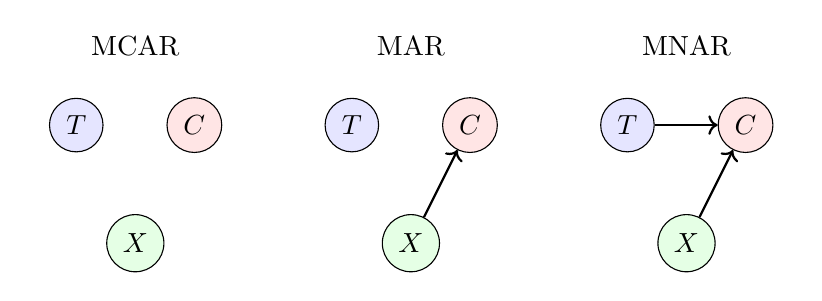
\begin{tikzpicture}
        % MCAR diagram
        \begin{scope}[shift={(-3.5,0)}]
            \node[draw, circle, fill=blue!10] (T1) at (0,0) {$T$};
            \node[draw, circle, fill=red!10] (C1) at (1.5,0) {$C$};
            \node[draw, circle, fill=green!10] (X1) at (0.75,-1.5) {$X$};

            \node[align=center, text width=2.5cm] at (0.75,1) {MCAR};
        \end{scope}

        % MAR diagram
        \begin{scope}[shift={(0,0)}]
            \node[draw, circle, fill=blue!10] (T2) at (0,0) {$T$};
            \node[draw, circle, fill=red!10] (C2) at (1.5,0) {$C$};
            \node[draw, circle, fill=green!10] (X2) at (0.75,-1.5) {$X$};

            \draw[->, thick] (X2) -- (C2);

            \node[align=center, text width=2.5cm] at (0.75,1) {MAR};
        \end{scope}

        % MNAR diagram
        \begin{scope}[shift={(3.5,0)}]
            \node[draw, circle, fill=blue!10] (T3) at (0,0) {$T$};
            \node[draw, circle, fill=red!10] (C3) at (1.5,0) {$C$};
            \node[draw, circle, fill=green!10] (X3) at (0.75,-1.5) {$X$};

            \draw[->, thick] (X3) -- (C3);
            \draw[->, thick] (T3) -- (C3);

            \node[align=center, text width=2.5cm] at (0.75,1) {MNAR};
        \end{scope}
    \end{tikzpicture}
    \caption{Directed acyclic graphs illustrating different censoring mechanisms. Arrows indicate dependencies between variables. Under MCAR, censoring is independent of other variables. Under MAR, censoring depends on observed covariates. Under MNAR, censoring depends on the unobserved event time.}
    \label{fig:censoring-mechanisms}
\end{figure}

\begin{notebox}[title=Non-informative vs. Informative Censoring]
A related distinction is between:
\begin{itemize}
    \item \textbf{Non-informative censoring:} The censoring process provides no information about the event time beyond what is available in the observed covariates (equivalent to MCAR or MAR)
    \item \textbf{Informative censoring:} The censoring process itself provides information about the event time (equivalent to MNAR)
\end{itemize}

Most standard survival methods assume non-informative censoring. When censoring is informative, more complex joint modeling of the censoring and event processes may be required.
\end{notebox}

For survival analysis methods to produce valid results, censoring must typically be:

\begin{itemize}
    \item \textbf{Independent/non-informative:} The censoring mechanism should be unrelated to the event process. If subjects who are more likely to experience the event are also more likely to be censored, we have informative censoring, which can bias results.

    \item \textbf{Random:} The distribution of censoring times should be random and not systematically related to subject characteristics or study conditions.
\end{itemize}

These assumptions should be critically evaluated in any survival analysis. When they're violated, sensitivity analyses or models that account for informative censoring may be needed.

\section{Competing Risks}
\label{sec:competing-risks}

Competing risks occur when subjects can experience multiple types of events, and the occurrence of one event precludes the occurrence of other events or changes their probability. Traditional survival analysis methods that treat competing events as censored can lead to biased estimates.

\begin{figure}[htbp]
    \centering
    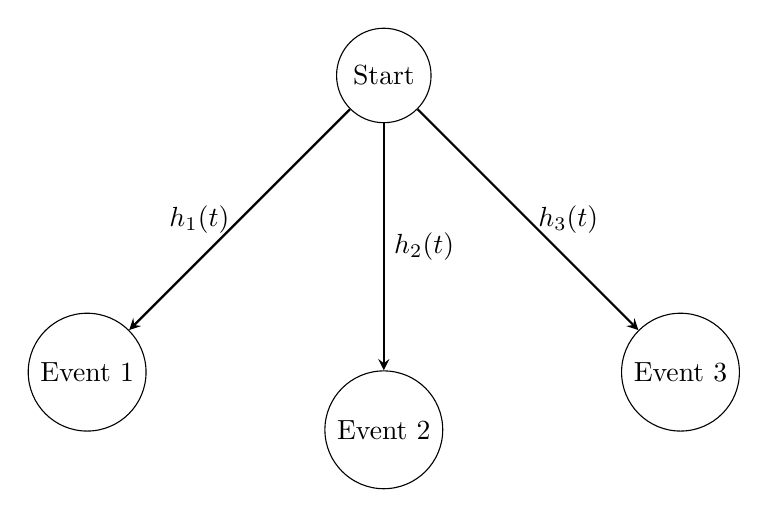
\begin{tikzpicture}[
        node distance=2.5cm,
        state/.style={circle, draw, minimum size=1.2cm},
        arrow/.style={->, >=stealth, thick}
    ]
        % States
        \node[state] (start) at (0,0) {Start};
        \node[state, below left of=start] (event1) at (-2,-2) {Event 1};
        \node[state, below of=start] (event2) at (0,-2) {Event 2};
        \node[state, below right of=start] (event3) at (2,-2) {Event 3};

        % Transitions
        \draw[arrow] (start) -- (event1) node[midway, left] {$h_1(t)$};
        \draw[arrow] (start) -- (event2) node[midway, right] {$h_2(t)$};
        \draw[arrow] (start) -- (event3) node[midway, right] {$h_3(t)$};
    \end{tikzpicture}
    \caption{Competing risks framework. From the initial state, a subject can transition to one of several possible event states, each with its own hazard function. Once one event occurs, the subject is no longer at risk for the other events.}
    \label{fig:competing-risks}
\end{figure}

\subsection{Analyzing Competing Risks}
\label{subsec:analyzing-competing-risks}

When analyzing data with competing risks, we consider:

\begin{itemize}
    \item \textbf{Cause-specific hazards:} The instantaneous rate of occurrence of a specific event type among those still at risk.

    \item \textbf{Cumulative Incidence Function (CIF):} The probability of experiencing a specific event type before time $t$ and before experiencing any competing event.

    \item \textbf{Subdistribution hazard:} The instantaneous rate of occurrence of a specific event type among those who have not experienced that specific event yet (including those who have experienced competing events).
\end{itemize}

Unlike in the standard survival setting where the survival function is directly related to the hazard, in competing risks, the relationship between cause-specific hazards and CIFs is more complex. A reduction in one cause-specific hazard may not necessarily translate to an increase in the corresponding CIF due to the interplay with competing events.

\subsection{Modeling Approaches for Competing Risks}
\label{subsec:modeling-competing-risks}

\begin{itemize}
    \item \textbf{Cause-specific Cox models:} Fit separate Cox models for each cause, treating competing events as censored.

    \item \textbf{Fine and Gray model:} Models the subdistribution hazard directly, allowing for direct assessment of covariate effects on the CIF.

    \item \textbf{Multi-state models:} Consider transitions between different states (e.g., healthy, diseased, dead) and can model complex disease processes.

    \item \textbf{Joint modeling:} Simultaneously model multiple event types, accounting for their dependencies.

    \item \textbf{Neural approaches (e.g., MENSA):} Use neural networks to model complex relationships between covariates and multiple event types.
\end{itemize}

The choice of method depends on the research question—whether the interest is in etiology (cause-specific hazards) or absolute risk prediction (CIFs).

\begin{examplebox}[title=Examples of Competing Risks]
  \begin{itemize}
  \item In medical studies: Death from cancer, heart disease, or other causes
  \item In engineering: Component failure due to wear, corrosion, or manufacturing defect
  \item In business: Customer churn due to price, service quality, or competitor offers
  \item In employment: Job termination due to retirement, new job opportunity, or layoff
  \end{itemize}
\end{examplebox}

\begin{notebox}[title=Important Note on Competing Risks]
A critical point in competing risks analysis is that $1 - S_j(t) \neq F_j(t)$, where $S_j(t)$ is the cause-specific survival function obtained by treating other event types as censored.

The Kaplan-Meier estimator applied to a single event type (treating others as censored) overestimates the probability of that event in the presence of competing risks.
\end{notebox}


\chapter{Deep Survival Machines}
\label{ch:dsm}
\section{Introduction to Deep Survival Machines}

Deep Survival Machines (DSM) \parencite{nagpal2021dsm} represents a paradigm shift in survival analysis, introducing a novel approach that bridges the gap between traditional statistical methods and modern deep learning. This chapter explores how DSM combines the strengths of neural networks with parametric survival modeling to overcome the limitations of both conventional approaches \parencite{cox1972,kaplan1958} and earlier neural network adaptations for survival analysis \parencite{katzman2018,chapfuwa2018}.

\begin{notebox}[title=Chapter Overview]
This chapter covers:
\begin{itemize}
    \item The limitations of traditional survival analysis methods
    \item Complex hazard patterns in real-world survival data
    \item The conceptual innovation of the DSM mixture approach
    \item Mathematical foundations of DSM
    \item Implementation details and practical considerations
    \item Advantages of DSM over alternative methods
    \item Applications and results in real-world scenarios
\end{itemize}
\end{notebox}

\section{Limitations of Traditional Survival Analysis Methods}

Despite the theoretical foundations discussed in the previous chapter, traditional survival analysis methods face significant limitations when applied to complex, high-dimensional real-world data. Understanding these limitations provides the motivation for developing more advanced approaches like Deep Survival Machines.

\subsection{Limitations of Non-parametric Methods}

The Kaplan-Meier estimator and other non-parametric methods, while making minimal assumptions about the underlying distribution, have several important constraints:

\begin{itemize}
    \item \textbf{Limited covariate handling:} They cannot effectively incorporate continuous covariates or high-dimensional feature spaces
    \item \textbf{Reliance on stratification:} Covariate adjustment is limited to stratification by categorical variables, which quickly becomes impractical with multiple variables
    \item \textbf{No extrapolation:} Predictions cannot extend beyond the largest observed event time in the dataset
    \item \textbf{Curse of dimensionality:} Performance degrades in high-dimensional settings
    \item \textbf{Inefficient use of data:} Cannot leverage patterns across different strata
\end{itemize}

\subsection{Limitations of the Cox Proportional Hazards Model}

While the Cox model addresses some limitations of non-parametric methods by enabling covariate adjustment, it introduces its own constraints:

\begin{itemize}
    \item \textbf{Proportional hazards assumption:} Assumes that the hazard ratio between any two subjects remains constant over time—an assumption frequently violated in practice
    \item \textbf{Linear effects:} Assumes that covariates have a log-linear effect on the hazard, which may not capture complex non-linear relationships
    \item \textbf{Baseline hazard challenges:} The baseline hazard estimation is often unstable, especially with sparse data at longer follow-up times
    \item \textbf{Time-varying effects:} Accommodating time-varying covariate effects requires complex model extensions
    \item \textbf{Limited interaction modeling:} Capturing complex interactions between covariates requires explicit specification
\end{itemize}

\subsection{Limitations of Early Neural Network Adaptations}

Early efforts to apply neural networks to survival analysis, while promising, retained significant limitations:

\begin{itemize}
    \item \textbf{Specialized architectures:} Required complex, specialized architectures to handle censored data
    \item \textbf{Proportional hazards heritage:} Many approaches still relied on the proportional hazards assumption
    \item \textbf{Black-box nature:} Limited interpretability and uncertainty quantification
    \item \textbf{Numerical challenges:} Suffered from instability in optimization and prediction
    \item \textbf{Distribution constraints:} Often still constrained to specific parametric forms or semi-parametric assumptions
\end{itemize}

These limitations highlight the need for a more flexible approach that can leverage the representational power of neural networks while respecting the unique characteristics of survival data.

\section{Complex Hazard Patterns in Real-World Data}

Real-world survival data often exhibits complex hazard patterns that cannot be adequately captured by traditional models, which typically assume simple monotonic hazard functions.

\subsection{Multi-Modal Hazard Functions}

Many real-world processes, particularly in medicine, show hazard patterns with multiple modes or complex shapes:

\begin{itemize}
    \item \textbf{Early high risk followed by plateau:} Common in post-surgical scenarios where immediate complications dominate early risk
    \item \textbf{Delayed risk that increases over time:} Seen in certain cancers where recurrence risk grows after an initial treatment response
    \item \textbf{Multiple risk peaks (biphasic patterns):} Observed in diseases with distinct phases, such as certain autoimmune conditions
    \item \textbf{Risk patterns that vary by subpopulation:} Different risk profiles for different patient subgroups, even after controlling for observable covariates
\end{itemize}

\begin{figure}[htbp]
    \centering
    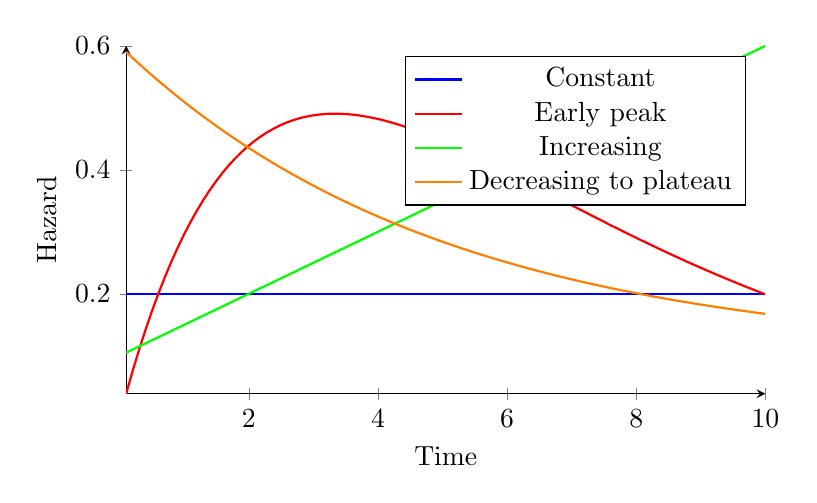
\begin{tikzpicture}
        \begin{axis}[
            width=0.8\textwidth,
            height=6cm,
            xlabel={Time},
            ylabel={Hazard},
            axis lines=left,
            domain=0.1:10,
            samples=100,
            legend pos=north east,
            ]
            % Different hazard shapes
            \addplot[blue, thick] {0.2}; % Constant
            \addplot[red, thick] {0.4*x*exp(-0.3*x)}; % Hump
            \addplot[green, thick] {0.1 + 0.05*x}; % Increasing
            \addplot[orange, thick] {0.5*exp(-0.2*x) + 0.1}; % Decreasing to plateau
            \legend{Constant, Early peak, Increasing, Decreasing to plateau}
        \end{axis}
    \end{tikzpicture}
    \caption{Examples of different hazard patterns observed in real-world survival data. Traditional models often assume a single pattern (such as constant or monotonically increasing/decreasing), but real processes frequently exhibit more complex behavior.}
    \label{fig:dsm-hazard-patterns}
\end{figure}

\subsection{The Need for Uncertainty Quantification}

Another critical limitation of many survival analysis methods is the lack of robust uncertainty quantification, which is essential in high-stakes decision-making contexts.

\begin{examplebox}[title=Clinical Decision-Making with Uncertainty]
Consider a physician deciding between aggressive and conservative treatment for a cancer patient:
\begin{itemize}
    \item A point estimate suggesting 60\% 5-year survival probability provides limited guidance
    \item Knowing the confidence interval is 40-80\% indicates substantial uncertainty
    \item This uncertainty information might lead to additional testing or consideration of patient preferences
    \item Without proper uncertainty quantification, decision-makers may have false confidence in predictions
\end{itemize}
\end{examplebox}

Two fundamental types of uncertainty need to be addressed:
\begin{itemize}
    \item \textbf{Epistemic uncertainty:} Uncertainty due to model limitations and finite data—can theoretically be reduced with more data or better models
    \item \textbf{Aleatoric uncertainty:} Inherent randomness in the process being modeled—cannot be reduced with more data and represents genuine outcome variability
\end{itemize}

\begin{figure}[htbp]
    \centering
    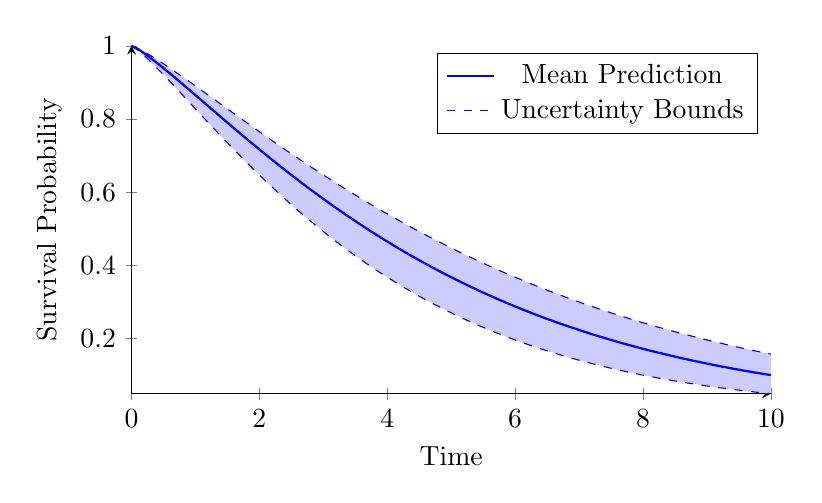
\begin{tikzpicture}
        \begin{axis}[
            width=0.8\textwidth,
            height=6cm,
            xlabel={Time},
            ylabel={Survival Probability},
            axis lines=left,
            domain=0:10,
            samples=100,
            ]
            % Mean prediction
            \addplot[blue, thick] {exp(-(x/5)^1.2)};

            % Upper and lower confidence bounds with named paths
            \addplot[blue, dashed, name path=upper] {exp(-(x/6)^1.2)};
            \addplot[blue, dashed, name path=lower] {exp(-(x/4)^1.2)};

            % Fill between the named paths
            \addplot[blue!20, forget plot] fill between[of=upper and lower];

            \legend{Mean Prediction, Uncertainty Bounds}
        \end{axis}
    \end{tikzpicture}
    \caption{Survival curve with uncertainty bounds. The shaded region represents the uncertainty in the survival estimates, which increases over time as less information is available. This visualization provides decision-makers with both the point estimate and a measure of confidence in that estimate.}
    \label{fig:survival-uncertainty}
\end{figure}

These complex hazard patterns and the need for robust uncertainty quantification motivate the development of more flexible and expressive approaches to survival analysis.

\section{Deep Survival Machines: Core Conceptual Innovation}

Deep Survival Machines introduces a novel approach to survival analysis that addresses the limitations of traditional methods while leveraging the representational power of neural networks.

\subsection{The Mixture Distribution Approach}

The central innovation of DSM is to model survival as a mixture of parametric distributions:

\begin{itemize}
    \item \textbf{Mixture composition:} The survival function is modeled as a weighted sum of multiple parametric survival functions
    \item \textbf{Component diversity:} Each component can capture a different risk pattern or represent a different subpopulation
    \item \textbf{Neural parameter mapping:} Neural networks learn to map from input features to distribution parameters and mixture weights
    \item \textbf{Flexible hazard representation:} The mixture approach can represent virtually any smooth hazard function
    \item \textbf{Natural uncertainty quantification:} The mixture variance provides a measure of predictive uncertainty
\end{itemize}

\begin{figure}[htbp]
    \centering
    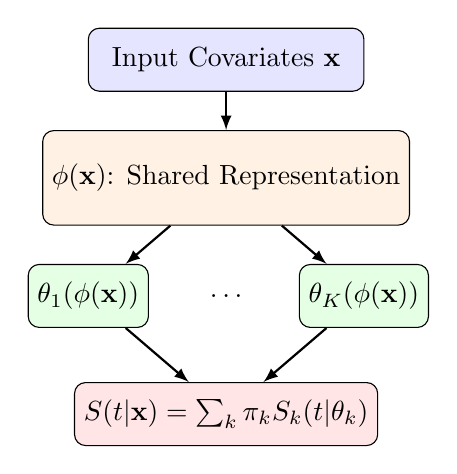
\begin{tikzpicture}[scale=1.0, transform shape]
        \node[draw, rounded corners, minimum width=3.5cm, minimum height=0.8cm, fill=blue!10] (input) at (0,0) {Input Covariates $\mathbf{x}$};

        \node[draw, rounded corners, minimum width=3.5cm, minimum height=1.2cm, fill=orange!10] (shared) at (0,-1.5) {$\phi(\mathbf{x})$: Shared Representation};

        \node[draw, rounded corners, minimum width=1.5cm, minimum height=0.8cm, fill=green!10] (k1) at (-1.75,-3) {$\theta_1(\phi(\mathbf{x}))$};
        \node at (0,-3) {$\ldots$};
        \node[draw, rounded corners, minimum width=1.5cm, minimum height=0.8cm, fill=green!10] (k2) at (1.75,-3) {$\theta_K(\phi(\mathbf{x}))$};

        \node[draw, rounded corners, minimum width=3.5cm, minimum height=0.8cm, fill=red!10] (output) at (0,-4.5) {$S(t|\mathbf{x}) = \sum_k \pi_k S_k(t|\theta_k)$};

        \draw[-latex, thick] (input) -- (shared);
        \draw[-latex, thick] (shared) -- (k1);
        \draw[-latex, thick] (shared) -- (k2);
        \draw[-latex, thick] (k1) -- (output);
        \draw[-latex, thick] (k2) -- (output);
    \end{tikzpicture}
    \caption{Conceptual architecture of Deep Survival Machines. Input covariates are processed through a shared representation layer, which then feeds into parameter networks for each mixture component. The final survival function is a weighted combination of the component survival functions.}
    \label{fig:dsm-architecture}
\end{figure}

\subsection{Architectural Components}

The DSM architecture consists of three main components that work together to create a flexible and expressive survival model:

\subsubsection{Representation Network}

The representation network transforms raw covariates into a latent feature representation:
\begin{itemize}
    \item Can use any neural network architecture appropriate for the data type (MLP for tabular data, CNN for images, transformers for sequential data, etc.)
    \item Learns task-relevant feature extraction and transformation
    \item Enables automatic feature learning and extraction of complex patterns
    \item Creates a shared representation that feeds into the parameter networks
\end{itemize}

\subsubsection{Mixture Model}

The mixture model combines multiple parametric survival distributions:
\begin{itemize}
    \item Typically uses 2-8 components, depending on data complexity
    \item Components are usually from the same parametric family (e.g., all Weibull) but with different parameters
    \item Models different risk patterns and subpopulations implicitly discovered from the data
    \item Creates a flexible composition that can represent complex hazard shapes
\end{itemize}

\subsubsection{Parameter Networks}

Parameter networks map from the shared representation to the parameters of each distribution component:
\begin{itemize}
    \item Separate networks for each parameter type (e.g., shape, scale) and each component
    \item Include constraints to ensure valid parameter ranges (e.g., positive shape parameters)
    \item Learn adaptive mixture weights that determine the contribution of each component
    \item Enable personalized parameter estimation based on individual covariates
\end{itemize}

\section{Key Innovations of Deep Survival Machines}

Deep Survival Machines introduces several key innovations that distinguish it from both traditional survival methods and earlier neural network approaches.

\subsection{End-to-End Learning}

Unlike many traditional survival models that separate feature engineering from survival modeling, DSM enables end-to-end learning:
\begin{itemize}
    \item Joint optimization of representation learning and survival parameter estimation
    \item No need for separate feature engineering or transformation steps
    \item Gradient-based optimization of all model components
    \item Representation automatically adapts to the survival prediction task
\end{itemize}

\subsection{Flexible Hazard Modeling}

The mixture approach enables modeling of complex hazard patterns without restrictive assumptions:
\begin{itemize}
    \item No proportional hazards assumption required
    \item Can model virtually any survival distribution
    \item Automatically captures non-linear relationships between covariates and survival
    \item Adapts to the underlying data-generating process
\end{itemize}

\subsection{Uncertainty Quantification}

DSM provides natural uncertainty quantification through its mixture formulation:
\begin{itemize}
    \item The mixture variance provides a measure of predictive uncertainty
    \item Different components can represent different risk scenarios
    \item Uncertainty can be visualized through prediction intervals
    \item Both epistemic and aleatoric uncertainty are captured
\end{itemize}

\subsection{Risk Prediction Capabilities}

Unlike many survival models that focus on relative risks, DSM provides comprehensive risk assessment:
\begin{itemize}
    \item Direct probability outputs (not just relative risks)
    \item Time-dependent risk assessment at any time point
    \item Personalized survival curves for individual subjects
    \item Risk stratification based on predicted outcomes
\end{itemize}

\section{Mathematical Foundation of Deep Survival Machines}

To fully understand DSM, we need to examine its mathematical formulation, starting with the basic survival analysis functions and extending to the mixture framework.

\subsection{Survival Analysis Fundamentals: A Brief Recap}

As discussed in the previous chapter, for a random variable $T$ representing survival time, the key probability functions are:

\begin{equationbox}[title=Core Survival Functions]
\begin{align}
    \text{Survival function: } & S(t) = P(T > t) \\
    \text{CDF: } & F(t) = P(T \leq t) = 1 - S(t) \\
    \text{PDF: } & f(t) = \frac{d}{dt}F(t) = -\frac{d}{dt}S(t) \\
    \text{Hazard function: } & h(t) = \frac{f(t)}{S(t)} = -\frac{d}{dt}\log S(t) \\
    \text{Cumulative hazard: } & H(t) = \int_0^t h(u) du = -\log S(t)
\end{align}
\end{equationbox}

These functions are interrelated, and each provides a different perspective on the time-to-event process. DSM builds on this foundation by introducing a mixture framework.

\subsection{The Mixture Framework}

The fundamental insight of DSM is to model the survival distribution as a mixture of parametric distributions:

\begin{equationbox}[title=DSM Mixture Survival Function]
\begin{align}
    S(t|\mathbf{x}) &= \sum_{k=1}^{K} \pi_k(\mathbf{x}) S_k(t|\mathbf{x})
\end{align}

where:
\begin{itemize}
    \item $S(t|\mathbf{x})$ is the overall survival function given covariates $\mathbf{x}$
    \item $S_k(t|\mathbf{x})$ is the survival function for the $k$-th component
    \item $\pi_k(\mathbf{x})$ is the mixture weight for the $k$-th component
    \item $\sum_{k=1}^K \pi_k(\mathbf{x}) = 1$ and $\pi_k(\mathbf{x}) \geq 0$ for all $k$
\end{itemize}
\end{equationbox}

From this mixture survival function, we can derive the corresponding density and hazard functions:

\begin{equationbox}[title=DSM Mixture Density and Hazard]
\begin{align}
    f(t|\mathbf{x}) &= -\frac{d}{dt}S(t|\mathbf{x}) = \sum_{k=1}^{K} \pi_k(\mathbf{x}) f_k(t|\mathbf{x}) \\
    h(t|\mathbf{x}) &= \frac{f(t|\mathbf{x})}{S(t|\mathbf{x})} = \frac{\sum_{k=1}^{K} \pi_k(\mathbf{x}) f_k(t|\mathbf{x})}{\sum_{k=1}^{K} \pi_k(\mathbf{x}) S_k(t|\mathbf{x})}
\end{align}
\end{equationbox}

\subsection{Insight into Hazard Composition}

The mixture hazard can be rewritten to provide insight into how the different components contribute:

\begin{equationbox}[title=Alternative Hazard Formulation]
\begin{align}
    h(t|\mathbf{x}) &= \frac{\sum_{k=1}^{K} \pi_k(\mathbf{x}) f_k(t|\mathbf{x})}{\sum_{k=1}^{K} \pi_k(\mathbf{x}) S_k(t|\mathbf{x})} \\
    &= \sum_{k=1}^{K} \frac{\pi_k(\mathbf{x}) S_k(t|\mathbf{x})}{\sum_{j=1}^{K} \pi_j(\mathbf{x}) S_j(t|\mathbf{x})} h_k(t|\mathbf{x})
\end{align}
\end{equationbox}

This reveals that the overall hazard is a weighted combination of component hazards, where the weights change over time. The weighting factor $\frac{\pi_k S_k}{\sum_j \pi_j S_j}$ represents the posterior probability that an individual who survived to time $t$ belongs to component $k$.

\section{Parametric Component Distributions}

DSM can use various parametric distributions for its mixture components. The two most common choices are the Weibull and log-normal distributions.

\subsection{Weibull Distribution}

The Weibull distribution is frequently used due to its flexibility in modeling different hazard shapes:

\begin{equationbox}[title=Weibull Distribution Functions]
\begin{align}
    S_k(t|\mathbf{x}) &= \exp\left[-\left(\frac{t}{\lambda_k(\mathbf{x})}\right)^{\alpha_k(\mathbf{x})}\right] \\
    f_k(t|\mathbf{x}) &= \frac{\alpha_k(\mathbf{x})}{\lambda_k(\mathbf{x})}\left(\frac{t}{\lambda_k(\mathbf{x})}\right)^{\alpha_k(\mathbf{x})-1}\exp\left[-\left(\frac{t}{\lambda_k(\mathbf{x})}\right)^{\alpha_k(\mathbf{x})}\right] \\
    h_k(t|\mathbf{x}) &= \frac{\alpha_k(\mathbf{x})}{\lambda_k(\mathbf{x})}\left(\frac{t}{\lambda_k(\mathbf{x})}\right)^{\alpha_k(\mathbf{x})-1}
\end{align}

where:
\begin{itemize}
    \item $\lambda_k(\mathbf{x})$ is the scale parameter, which influences the median survival time
    \item $\alpha_k(\mathbf{x})$ is the shape parameter, which determines the hazard behavior
\end{itemize}
\end{equationbox}

The shape parameter $\alpha_k$ controls the hazard shape in a Weibull distribution:
\begin{itemize}
    \item $\alpha_k = 1$: Constant hazard (exponential distribution)
    \item $\alpha_k > 1$: Increasing hazard (e.g., wear-out, aging)
    \item $\alpha_k < 1$: Decreasing hazard (e.g., early failures, infections)
\end{itemize}

\begin{figure}[htbp]
    \centering
    \begin{tikzpicture}
        \begin{axis}[
            width=0.8\textwidth,
            height=6cm,
            xlabel={Time},
            ylabel={Hazard},
            axis lines=left,
            domain=0.1:5,
            samples=100,
            legend style={at={(0.05,0.95)}, anchor=north west},
            ]
            \addplot[blue, thick] {1/2};
            \addplot[red, thick] {2/2*(x/2)^1};
            \addplot[green, thick] {0.25/sqrt(x/2)};
            \legend{Shape 1, Shape 2, Shape 0.5}
        \end{axis}
    \end{tikzpicture}
    \caption{Weibull hazard functions with different shape parameters. When $\alpha = 1$ (blue), the hazard is constant. When $\alpha > 1$ (red), the hazard increases with time. When $\alpha < 1$ (green), the hazard decreases with time.}
    \label{fig:weibull-hazards}
\end{figure}

\subsection{Log-Normal Distribution}

DSM can also use log-normal components, which provide different hazard characteristics:

\begin{equationbox}[title=Log-Normal Distribution Functions]
\begin{align}
    S_k(t|\mathbf{x}) &= 1 - \Phi\left(\frac{\log t - \mu_k(\mathbf{x})}{\sigma_k(\mathbf{x})}\right) \\
    f_k(t|\mathbf{x}) &= \frac{1}{t\sigma_k(\mathbf{x})\sqrt{2\pi}}\exp\left(-\frac{(\log t - \mu_k(\mathbf{x}))^2}{2\sigma_k^2(\mathbf{x})}\right) \\
    h_k(t|\mathbf{x}) &= \frac{f_k(t|\mathbf{x})}{S_k(t|\mathbf{x})}
\end{align}

where:
\begin{itemize}
    \item $\mu_k(\mathbf{x})$ is the location parameter
    \item $\sigma_k(\mathbf{x})$ is the scale parameter
    \item $\Phi$ is the standard normal cumulative distribution function
\end{itemize}
\end{equationbox}

The log-normal distribution has distinct characteristics:
\begin{itemize}
    \item Non-monotonic hazard that increases and then decreases
    \item Better for modeling certain diseases with delayed effects
    \item More parameters to optimize
    \item Often used for modeling cancer survival with delayed treatment effects
\end{itemize}

\subsection{The Power of Mixtures}

The mixture approach allows DSM to model complex hazard patterns that would be impossible with a single parametric distribution. With just 2-4 components, DSM can represent:

\begin{itemize}
    \item Bathtub hazards (high early risk, low middle, high late)
    \item Multi-modal hazards (multiple risk peaks)
    \item U-shaped hazards
    \item Virtually any smooth hazard function
\end{itemize}

\begin{figure}[htbp]
    \centering
    \begin{tikzpicture}
        \begin{axis}[
            width=0.8\textwidth,
            height=6cm,
            xlabel={Time},
            ylabel={Hazard},
            axis lines=left,
            domain=0.1:10,
            samples=200,
            legend pos=north east,
            ]
            % Bathtub hazard (high early, low middle, rising late)
            \addplot[blue, thick] {0.5*exp(-0.5*x) + 0.05*x + 0.1};

            % Bimodal hazard (two peaks)
            \addplot[red, thick] {0.4*x*exp(-0.5*x) + 0.2*(x-6)^2*exp(-2*(x-6)^2) + 0.1};

            \legend{Bathtub Hazard, Bimodal Hazard}
        \end{axis}
    \end{tikzpicture}
    \caption{Complex hazard patterns that can be modeled using mixtures of simple parametric distributions. The bathtub pattern (blue) shows high initial risk, followed by a stable period, and then increasing risk. The bimodal pattern (red) shows two distinct risk peaks.}
    \label{fig:complex-hazards}
\end{figure}

\section{Neural Parameter Mapping}

A key aspect of DSM is the use of neural networks to map from input features to distribution parameters.

\subsection{From Features to Distribution Parameters}

DSM employs a series of neural network transformations to derive distribution parameters from input features:

\begin{equationbox}[title=Neural Parameter Mapping]
\begin{align}
    \phi(\mathbf{x}) &= \text{neural\_network}(\mathbf{x}) \\
    \alpha_k(\mathbf{x}) &= \text{softplus}(w_{\alpha_k}^T \phi(\mathbf{x}) + b_{\alpha_k}) + \varepsilon \\
    \lambda_k(\mathbf{x}) &= \text{softplus}(w_{\lambda_k}^T \phi(\mathbf{x}) + b_{\lambda_k}) + \varepsilon \\
    \tilde{\pi}_k(\mathbf{x}) &= w_{\pi_k}^T \phi(\mathbf{x}) + b_{\pi_k} \\
    \pi_k(\mathbf{x}) &= \frac{\exp(\tilde{\pi}_k(\mathbf{x}))}{\sum_{j=1}^{K} \exp(\tilde{\pi}_j(\mathbf{x}))}
\end{align}

where:
\begin{itemize}
    \item $\phi(\mathbf{x})$ is the shared representation from the neural network
    \item $w_{\alpha_k}$, $w_{\lambda_k}$, $w_{\pi_k}$ are parameter-specific weights
    \item $b_{\alpha_k}$, $b_{\lambda_k}$, $b_{\pi_k}$ are parameter-specific biases
    \item softplus activation ensures positive values for $\alpha_k$ and $\lambda_k$
    \item softmax ensures mixture weights $\pi_k$ sum to 1
    \item $\varepsilon$ is a small positive constant (e.g., 0.01) to prevent numerical issues
\end{itemize}
\end{equationbox}

\subsection{Network Architecture}

The complete DSM architecture can be visualized as follows:

\begin{figure}[htbp]
    \centering
    \begin{tikzpicture}
        \node[draw, rounded corners, minimum width=4cm, minimum height=0.8cm, fill=blue!10] (input) at (0,0) {$\mathbf{x} \in \mathbb{R}^d$};

        \node[draw, rounded corners, minimum width=4cm, minimum height=0.8cm, fill=orange!10] (hidden1) at (0,-1.5) {$\mathbf{h}_1 = \sigma(W_1\mathbf{x} + \mathbf{b}_1)$};

        \node[draw, rounded corners, minimum width=4cm, minimum height=0.8cm, fill=orange!10] (hidden2) at (0,-2.7) {$\phi(\mathbf{x}) = \sigma(W_2\mathbf{h}_1 + \mathbf{b}_2)$};

        \node[draw, rounded corners, minimum width=2.5cm, minimum height=0.8cm, fill=green!10] (alpha) at (-3,-4) {$\alpha_k(\mathbf{x})$};

        \node[draw, rounded corners, minimum width=2.5cm, minimum height=0.8cm, fill=green!10] (lambda) at (0,-4) {$\lambda_k(\mathbf{x})$};

        \node[draw, rounded corners, minimum width=2.5cm, minimum height=0.8cm, fill=green!10] (pi) at (3,-4) {$\pi_k(\mathbf{x})$};

        \draw[-latex, thick] (input) -- (hidden1);
        \draw[-latex, thick] (hidden1) -- (hidden2);
        \draw[-latex, thick] (hidden2) -- (alpha);
        \draw[-latex, thick] (hidden2) -- (lambda);
        \draw[-latex, thick] (hidden2) -- (pi);
    \end{tikzpicture}
    \caption{Neural network architecture for DSM. Input features are processed through shared hidden layers to create a representation $\phi(\mathbf{x})$, which is then fed into parameter-specific output heads to generate distribution parameters and mixture weights.}
    \label{fig:dsm-network}
\end{figure}

\section{Training Deep Survival Machines}

Training DSM involves defining an appropriate loss function and addressing several numerical challenges.

\subsection{Loss Function Formulation}

For censored survival data:
\begin{itemize}
    \item If event observed ($\delta_i = 1$): Time $t_i$ is the exact event time
    \item If censored ($\delta_i = 0$): Event occurs after $t_i$ (right censoring)
\end{itemize}

The likelihood contribution for each observation is:
\begin{align}
    L_i = [f(t_i|\mathbf{x}_i)]^{\delta_i} \cdot [S(t_i|\mathbf{x}_i)]^{1-\delta_i}
\end{align}

Taking the negative log of the likelihood and expanding:
\begin{align}
    -\log L_i &= -\delta_i \log f(t_i|\mathbf{x}_i) - (1-\delta_i) \log S(t_i|\mathbf{x}_i) \\
    &= -\delta_i \log \left[\sum_{k=1}^{K} \pi_k(\mathbf{x}_i) f_k(t_i|\mathbf{x}_i)\right] \\
    &\quad - (1-\delta_i) \log \left[\sum_{k=1}^{K} \pi_k(\mathbf{x}_i) S_k(t_i|\mathbf{x}_i)\right]
\end{align}

The full loss is then the sum over all observations:
\begin{align}
    \mathcal{L}_{DSM} = \sum_{i=1}^N -\log L_i
\end{align}

\subsection{ELBO-Based Regularization}

Mixture models can suffer from component collapse, where all weight concentrates in just one component. To encourage the use of multiple components and create more diverse representations, DSM employs an Evidence Lower Bound (ELBO) regularization approach.

From a latent variable perspective, we can view $k$ as a latent mixture component:
\begin{align}
    \log p(t|\mathbf{x}) &= \log \sum_{k=1}^K p(t, k|\mathbf{x}) = \log \sum_{k=1}^K p(t|k,\mathbf{x})p(k|\mathbf{x}) \\
    &\geq \sum_{k=1}^K q(k|\mathbf{x}) \log \frac{p(t|k,\mathbf{x})p(k|\mathbf{x})}{q(k|\mathbf{x})} \\
    &= \sum_{k=1}^K q(k|\mathbf{x}) \log p(t|k,\mathbf{x}) - \sum_{k=1}^K q(k|\mathbf{x}) \log \frac{q(k|\mathbf{x})}{p(k|\mathbf{x})} \\
    &= \mathbb{E}_{q(k|\mathbf{x})}[\log p(t|k,\mathbf{x})] - KL(q(k|\mathbf{x})||p(k|\mathbf{x}))
\end{align}

If we use a uniform prior $p(k|\mathbf{x}) = 1/K$, the KL term becomes:
\begin{align}
    KL(q(k|\mathbf{x})||p(k|\mathbf{x})) = \sum_{k=1}^K q(k|\mathbf{x}) \log(K \cdot q(k|\mathbf{x}))
\end{align}

This motivates the ELBO regularizer that encourages diverse component usage:
\begin{align}
    \mathcal{L}_{ELBO} = \mathcal{L}_{DSM} + \beta \cdot KL(\pi(\mathbf{x})||\text{Uniform})
\end{align}

Where:
\begin{itemize}
    \item $\beta$ is a hyperparameter controlling regularization strength
    \item $\pi(\mathbf{x})$ is used as the $q(k|\mathbf{x})$ distribution
    \item This pushes mixture weights toward a uniform distribution
\end{itemize}

\section{Implementation Challenges and Solutions}

Implementing DSM involves addressing several numerical challenges to ensure stability and good performance.

\subsection{Numerical Stability Challenges}

The mixture likelihood calculation can encounter several numerical issues:
\begin{itemize}
    \item Overflow/underflow in exponential calculations
    \item Division by zero risk in hazard calculations
    \item Gradient explosion during backpropagation
    \item Parameter values spanning many orders of magnitude
\end{itemize}

\subsection{Log-Sum-Exp Trick}

For stable computation of $\log \sum_i e^{x_i}$, the log-sum-exp trick is essential:
\begin{align}
    \log \sum_i e^{x_i} &= \log \left[ e^a \sum_i e^{x_i - a}\right] \\
    &= a + \log \sum_i e^{x_i - a}
\end{align}
where $a = \max_i x_i$

This avoids underflow/overflow by bringing values to a numerically stable range.

\subsection{Gradient Detachment Strategy}

The gradient of the Weibull hazard with respect to the shape parameter $\alpha$ can explode for small time values when $\alpha < 1$:
\begin{align}
    \frac{\partial h(t|\alpha, \lambda)}{\partial \alpha} &= \frac{\partial}{\partial \alpha}\left[\frac{\alpha}{\lambda}\left(\frac{t}{\lambda}\right)^{\alpha-1}\right] \\
    &= \frac{1}{\lambda}\left(\frac{t}{\lambda}\right)^{\alpha-1} + \frac{\alpha}{\lambda}\left(\frac{t}{\lambda}\right)^{\alpha-1}\ln\left(\frac{t}{\lambda}\right)
\end{align}

To address gradient explosion, DSM implements a gradient detachment strategy:
\begin{enumerate}
    \item Identify potentially unstable operations
    \item Create a mask for extreme values
    \item Detach gradient computation for these values
    \item Use a weighted combination approach:
    \begin{align}
        result &= (1 - mask) \cdot normal\_result + mask \cdot detached\_result \\
        mask &= \mathbb{I}(|x| > threshold).float()
    \end{align}
\end{enumerate}

This allows learning to continue for stable values while preventing NaN gradients.

\section{Advantages of DSM over Traditional Methods}

DSM offers several key advantages over traditional survival analysis approaches, making it particularly suitable for complex, high-dimensional datasets.

\subsection{Compared to Cox Proportional Hazards}

\begin{itemize}
    \item \textbf{Flexibility:} Can model non-proportional hazards
    \item \textbf{Risk estimation:} Provides absolute risk estimates, not just relative
    \item \textbf{Feature learning:} Automatically learns non-linear feature interactions
    \item \textbf{Time prediction:} Directly models time-to-event distribution
    \item \textbf{Complex patterns:} Can capture non-monotonic hazard patterns
\end{itemize}

\subsection{Compared to Neural Cox Models}

Neural Cox models apply neural networks to learn features but still maintain the proportional hazards assumption. DSM offers advantages:
\begin{itemize}
    \item \textbf{No baseline estimation:} No baseline hazard estimation needed
    \item \textbf{Extrapolation:} Better extrapolation beyond training data
    \item \textbf{Uncertainty quantification:} Natural uncertainty quantification
    \item \textbf{Hazard flexibility:} Can model virtually any hazard pattern
    \item \textbf{Direct time modeling:} Models time directly rather than through hazards
\end{itemize}

\subsection{Compared to Random Survival Forests}

\begin{itemize}
    \item \textbf{End-to-end learning:} Differentiable learning instead of greedy splits
    \item \textbf{High-dimensional data:} Better handling of high-dimensional feature spaces
    \item \textbf{Representation learning:} More flexible feature learning
    \item \textbf{Computational efficiency:} More efficient after training
    \item \textbf{Scalability:} Better scalability to large datasets
\end{itemize}

\subsection{Limitations and Considerations}

While DSM offers many advantages, it also has limitations to consider:
\begin{itemize}
    \item \textbf{Distributional assumptions:} Requires choosing parametric component distributions
    \item \textbf{Computational intensity:} More computationally intensive to train than simpler models
    \item \textbf{Interpretability:} Less interpretable than simpler models, though mixture components can aid understanding
    \item \textbf{Implementation complexity:} Needs careful numerical implementation
    \item \textbf{Hyperparameters:} More hyperparameters to tune
\end{itemize}

\section{Practical Applications of DSM}

DSM has been successfully applied to various domains, demonstrating its practical utility.

\subsection{Cancer Survival Prediction}

One notable application is in breast cancer survival prediction using the METABRIC dataset:
\begin{itemize}
    \item Mixture of 4 Weibull distributions
    \item Neural network with 2 hidden layers
    \item Clinical and genomic features as input
    \item Shape parameters constrained to meaningful ranges for cancer progression
    \item Transformer-based feature embedding for handling complex feature interactions
\end{itemize}

Results showed significant improvements over traditional methods:
\begin{itemize}
    \item Higher C-index than Cox PH (0.67 vs 0.63)
    \item Better integrated Brier score
    \item Provided uncertainty intervals for risk stratification
    \item Identified distinct risk subgroups aligned with clinical knowledge
\end{itemize}

\begin{figure}[htbp]
    \centering
    \begin{tikzpicture}
        \begin{axis}[
            width=0.8\textwidth,
            height=6cm,
            xlabel={Time (years)},
            ylabel={Survival Probability},
            axis lines=left,
            domain=0:10,
            samples=100,
            legend style={at={(0.05,0.35)}, anchor=west},
            ]
            % High risk group
            \addplot[red, thick] {exp(-(x/3)^1.5)};
            % Medium risk group
            \addplot[orange, thick] {exp(-(x/5)^1.8)};
            % Low risk group
            \addplot[green, thick] {exp(-(x/7)^2.0)};
            \legend{High Risk, Medium Risk, Low Risk}
        \end{axis}
    \end{tikzpicture}
    \caption{Risk stratification using DSM for breast cancer patients. The model identifies distinct risk groups with different survival trajectories, enabling more personalized treatment planning.}
    \label{fig:risk-stratification}
\end{figure}

\section{Summary: DSM in the Bigger Picture}

Deep Survival Machines represents a significant advance in survival analysis, bridging the gap between traditional statistical methods and modern deep learning approaches.

\subsection{Key Contributions}

\begin{itemize}
    \item Combines neural networks with parametric survival distributions
    \item Models complex hazard shapes through the mixture approach
    \item Provides natural uncertainty quantification
    \item Bridges the gap between deep learning and survival analysis
    \item Enables personalized risk prediction with confidence intervals
\end{itemize}

\subsection{Future Directions}

The DSM framework opens several exciting avenues for future research:
\begin{itemize}
    \item Integration with causal inference frameworks
    \item Extension to interval censoring and competing risks (MENSA)
    \item Combination with advanced embedding techniques for different data modalities
    \item Application to federated learning settings for privacy-preserving analysis
    \item Incorporation of domain-specific prior knowledge to enhance predictions
\end{itemize}

\begin{notebox}[title=Looking Ahead]
In the next chapter, we will explore Multi-Event Neural Survival Analysis (MENSA), which extends the DSM framework to handle competing risks scenarios where subjects can experience different types of events. MENSA addresses the challenge of modeling dependencies between different event types while maintaining the flexibility and power of the DSM approach.
\end{notebox}


\chapter{Multi-Event Neural Survival Analysis}
\label{ch:mensa}
\section{Introduction to Multi-Event Neural Survival Analysis}

\subsection{The Big Picture: Moving Beyond Single-Event Survival}

In real-world scenarios, patients and systems often face multiple possible outcomes or failure modes \parencite{fine1999,prentice1978}. While traditional survival analysis typically focuses on a single event (like death or machine failure), many applications require modeling multiple competing or sequential events \parencite{austin2016,koller2012}. Multi-Event Neural Survival Analysis (MENSA) \parencite{zhong2021} addresses this challenge by extending the Deep Survival Machines (DSM) framework to handle competing risks scenarios.

\begin{notebox}[title=What is MENSA?]
MENSA (Multi-Event Neural Survival Analysis) is a deep learning framework designed to model time-to-event data with multiple possible events. It combines the flexible distribution-based approach of DSM with the ability to model dependencies between different event types.
\end{notebox}

MENSA brings several key advantages to survival analysis:

\begin{itemize}
    \item It models both event-specific patterns and inter-event dependencies
    \item It enables comprehensive risk prediction across multiple outcomes
    \item It bridges the gap between single-event survival and multi-state modeling
    \item It allows for information sharing across event types while maintaining event-specific characteristics
\end{itemize}

\begin{figure}[htbp]
    \centering
    \begin{tikzpicture}[
        scale=1.2,
        box/.style={draw, rounded corners, minimum width=3.5cm, minimum height=0.8cm, text centered},
        event/.style={draw, rounded corners, minimum width=1.5cm, minimum height=0.8cm, text centered, align=center},
        note/.style={draw, ellipse, minimum width=3cm, text centered},
        arrow/.style={->, >=latex, thick}
    ]
        % Basic MENSA architecture overview
        \node[box, fill=blue!10] (input) at (0,0) {Input Features $\mathbf{x}$};
        \node[box, fill=orange!10, minimum height=1.2cm] (mensa) at (0,-2) {MENSA};
        \node[event, fill=red!10] (e1) at (-3,-4) {Event 1\\Risk};
        \node[event, fill=red!10] (e2) at (0,-4) {Event 2\\Risk};
        \node[event, fill=red!10] (e3) at (3,-4) {Event J\\Risk};

        % Connections between components
        \draw[arrow] (input) -- (mensa);
        \draw[arrow] (mensa) -- (e1);
        \draw[arrow] (mensa) -- (e2);
        \draw[arrow] (mensa) -- (e3);

        % DSM connection note
        \node[note, fill=green!10] (dsm) at (-4,-1) {DSM};
        \draw[arrow, dashed] (dsm) -- (mensa);
        \node[right] at (-3.5,-1) {extends};

        % Multi-state connection note
        \node[note, fill=yellow!10] (ms) at (4,-1) {Multi-State Models};
        \draw[arrow, dashed] (ms) -- (mensa);
        \node[left] at (3.5,-1) {incorporates concepts from};
    \end{tikzpicture}
    \caption{Conceptual overview of the MENSA framework, showing its relationship to DSM and multi-state models, as well as its ability to model multiple event risks simultaneously.}
    \label{fig:mensa-overview}
\end{figure}

\subsection{Challenges in Multi-Event Survival Analysis}

Modeling multiple events introduces several challenges beyond those found in traditional single-event survival analysis:

\begin{itemize}
    \item \textbf{Multiple competing events:} Each event type may have distinct hazard profiles and risk factors
    \item \textbf{Complex dependencies:} Events can be interdependent, with the risk of one affecting the others
    \item \textbf{Data sparsity:} Individual events may have limited samples, requiring information sharing
    \item \textbf{Competing risk structure:} One event precludes the observation of others, creating informative censoring
    \item \textbf{Expert knowledge integration:} Each event may have domain-specific knowledge to incorporate
\end{itemize}

Figure \ref{fig:mensa-competing-risks-diagram} illustrates the competing risks structure, where a subject can transition from the initial state to one of several possible event states, but experiencing one event prevents observation of the others.

\begin{figure}[htbp]
    \centering
    \begin{tikzpicture}[
        scale=1.2,
        event/.style={circle, draw, thick, fill=blue!20, minimum size=1.2cm, text centered},
        arrow/.style={->, >=latex, thick}
    ]
        \node[event] (start) at (0,0) {Start};
        \node[event] (event1) at (-2.5,-2.5) {Event 1};
        \node[event] (event2) at (0,-2.5) {Event 2};
        \node[event] (event3) at (2.5,-2.5) {Event 3};

        \draw[arrow] (start) -- (event1) node[midway, above, sloped] {$h_1(t)$};
        \draw[arrow] (start) -- (event2) node[midway, right] {$h_2(t)$};
        \draw[arrow] (start) -- (event3) node[midway, above, sloped] {$h_3(t)$};

        \node[text width=2.5cm, align=center] at (-2.5,-3.5) {e.g., Cardiac Death};
        \node[text width=2.5cm, align=center] at (0,-3.5) {e.g., Cancer Death};
        \node[text width=2.5cm, align=center] at (2.5,-3.5) {e.g., Other Causes};

        % Challenge annotations
        \draw[red, thick, dashed, <->] (event1) to[bend right=20] node[below] {Dependencies} (event2);
        \draw[red, thick, dashed, <->] (event2) to[bend right=20] node[below] {Dependencies} (event3);

        % Competing nature visualization
        \node[draw, rounded corners, fill=yellow!10, align=center] at (0,1.5) {One event precludes others (competing risks)};
        \draw[->, dashed] (0,1.1) -- (0,0.6);
    \end{tikzpicture}
    \caption{Competing risks structure, showing transitions from a starting state to multiple possible events, with dependencies between events.}
    \label{fig:mensa-competing-risks-diagram}
\end{figure}

\section{The Competing Risks Framework}

\subsection{Data Representation in Competing Risks}

In the competing risks setting, each subject can experience one of $J$ different event types. We observe a triplet of information for each subject $i$:

\begin{definitionbox}[title=Competing Risks Data Structure]
For each subject $i$, we observe:
\begin{itemize}
    \item $T_i$: The observed time (either event time or censoring time)
    \item $J_i \in \{1, 2, \ldots, J\}$: The event type (if an event occurred)
    \item $\delta_i \in \{0, 1\}$: Censoring indicator (1 if event observed, 0 if censored)
\end{itemize}

If $\delta_i = 0$ (censored), then $J_i$ is undefined as no event has been observed.
\end{definitionbox}

Table \ref{tab:competing-risks-data} shows an example dataset with competing risks. Note how censored subjects (rows 3 and 5) have no defined event type.

\begin{table}[htbp]
    \centering
    \caption{Example of competing risks data structure}
    \label{tab:competing-risks-data}
    \begin{tabular}{@{}cccc@{}}
        \toprule
        Subject & Time $T_i$ & Event Type $J_i$ & Indicator $\delta_i$ \\
        \midrule
        1 & 3.5 & 1 & 1 \\
        2 & 5.0 & 2 & 1 \\
        3 & 7.0 & -- & 0 \\
        4 & 2.3 & 3 & 1 \\
        5 & 4.2 & -- & 0 \\
        \bottomrule
    \end{tabular}
\end{table}

In this example:
\begin{itemize}
    \item Subject 1 experienced event type 1 at time 3.5
    \item Subject 2 experienced event type 2 at time 5.0
    \item Subject 3 was censored at time 7.0 without experiencing any event
    \item Subject 4 experienced event type 3 at time 2.3
    \item Subject 5 was censored at time 4.2 without experiencing any event
\end{itemize}

\subsection{Censoring in Competing Risks}

Censoring becomes more complex in the competing risks setting. We need to distinguish between:

\begin{itemize}
    \item \textbf{Administrative censoring}: The study ended before any event was observed
    \item \textbf{Competing event censoring}: A different event occurred, which precludes observation of the event of interest
\end{itemize}

\begin{figure}[htbp]
    \centering
    \begin{tikzpicture}[scale=1.1]
        % Timeline
        \draw[->] (0,0) -- (10,0) node[right] {Time};
        \draw (0,0) node[below] {0};

        % Patient 1: Event 1
        \draw[ultra thick, -] (0,2.5) -- (3.5,2.5);
        \draw (3.5,2.5) node[circle, fill=red, inner sep=2pt] {};
        \node[right] at (3.5,2.5) {Event 1};

        % Patient 2: Event 2
        \draw[ultra thick, -] (0,2) -- (5,2);
        \draw (5,2) node[circle, fill=blue, inner sep=2pt] {};
        \node[right] at (5,2) {Event 2};

        % Patient 3: Censored
        \draw[ultra thick, -] (0,1.5) -- (7,1.5);
        \draw (7,1.5) node[circle, draw, fill=white, inner sep=2pt] {};
        \node[right] at (7,1.5) {Censored};

        % Event types legend
        \node[left] at (0,0.5) {Legend:};
        \draw (1,0.5) node[circle, fill=red, inner sep=2pt] {};
        \node[right] at (1.2,0.5) {Event 1 (e.g., Cardiac)};
        \draw (4,0.5) node[circle, fill=blue, inner sep=2pt] {};
        \node[right] at (4.2,0.5) {Event 2 (e.g., Cancer)};
        \draw (7,0.5) node[circle, draw, fill=white, inner sep=2pt] {};
        \node[right] at (7.2,0.5) {Administrative censoring};

        % Annotations for censoring types
        \draw[<->, dashed] (8.5,2.5) -- (8.5,1.5) node[midway, right, align=center] {Event 1 censors\\observation of\\Event 2};
        \draw[dashed, rounded corners] (6.5,1.3) rectangle (10,1.7);
        \node[below] at (8.25,1.3) {Administrative censoring};
    \end{tikzpicture}
    \caption{Illustration of censoring in competing risks. The occurrence of Event 1 prevents observing whether Event 2 would have occurred, creating a form of informative censoring specific to competing risks.}
    \label{fig:competing-risks-censoring}
\end{figure}

This distinction is crucial because competing event censoring is informative for the event of interest, unlike standard administrative censoring which is typically assumed to be non-informative. In Figure \ref{fig:competing-risks-censoring}, for Patient 1, we'll never know if or when Event 2 would have occurred because Event 1 happened first.

\section{Key Functions in Competing Risks}

To properly analyze competing risks data, we need to define several key functions that extend traditional survival analysis concepts.

\subsection{Cause-Specific Hazard Function}

\begin{definitionbox}[title=Cause-Specific Hazard]
The cause-specific hazard for event $j$ represents the instantaneous risk of experiencing event $j$ at time $t$, given survival (no events of any type) up to time $t$:

\begin{equation}
h_j(t) = \lim_{\Delta t \to 0} \frac{P(t \leq T < t + \Delta t, J = j | T \geq t)}{\Delta t}
\end{equation}
\end{definitionbox}

The cause-specific hazard can be interpreted as the rate at which event $j$ occurs at time $t$ among subjects who have not yet experienced any event. Each event type has its own hazard function, and these functions can have different shapes.

\begin{figure}[htbp]
    \centering
    \begin{tikzpicture}[scale=1.1]
        % Coordinate system
        \begin{axis}[
            width=0.8\textwidth,
            height=6cm,
            xlabel={Time},
            ylabel={Hazard Rate},
            axis lines=left,
            domain=0:10,
            samples=100,
            legend pos=north east,
            legend style={font=\small}
        ]
            % Independent cause-specific hazards
            \addplot[red, thick] {0.2};
            \addplot[blue, thick] {0.05*(x/2)};
            \addplot[green, thick] {0.1*exp(-0.1*x)};
            % Total hazard
            \addplot[black, thick, dashed] {0.2+0.05*(x/2)+0.1*exp(-0.1*x)};
            \legend{$h_1(t)$ (constant), $h_2(t)$ (increasing), $h_3(t)$ (decreasing), $h(t)$ (overall)}
        \end{axis}
    \end{tikzpicture}
    \caption{Cause-specific hazard functions for three different event types. Note how each event can have a distinct hazard pattern (constant, increasing, or decreasing over time).}
    \label{fig:cause-specific-hazards}
\end{figure}

Figure \ref{fig:cause-specific-hazards} shows three different cause-specific hazard functions:
\begin{itemize}
    \item Event 1: Constant hazard (exponential distribution)
    \item Event 2: Increasing hazard (e.g., Weibull with shape parameter > 1)
    \item Event 3: Decreasing hazard (e.g., Weibull with shape parameter < 1)
\end{itemize}

The overall hazard function $h(t)$ is the sum of all cause-specific hazards:

\begin{equationbox}
\begin{equation}
h(t) = \sum_{j=1}^{J} h_j(t)
\end{equation}
\end{equationbox}

\subsection{Overall Survival Function}

The overall survival function represents the probability of not experiencing any event up to time $t$. It depends on all cause-specific hazards:

\begin{equationbox}[title=Overall Survival Function]
\begin{equation}
S(t) = P(T > t) = \exp\left(-\sum_{j=1}^{J} \int_0^t h_j(u) du\right) = \exp\left(-\sum_{j=1}^{J} H_j(t)\right)
\end{equation}

where $H_j(t) = \int_0^t h_j(u) du$ is the cumulative hazard for event $j$.
\end{equationbox}

This equation shows how the overall survival is affected by all event types. If any cause-specific hazard increases, the overall survival decreases more rapidly. The survival function can be factorized as the product of survival functions specific to each event type, if we were hypothetically able to remove other competing risks:

\begin{equation}
S(t) = \exp(-H_1(t)) \cdot \exp(-H_2(t)) \cdot \ldots \cdot \exp(-H_J(t))
\end{equation}

\subsection{Cumulative Incidence Function}

The Cumulative Incidence Function (CIF) is central to competing risks analysis. Unlike in standard survival, we need a separate CIF for each event type.

\begin{definitionbox}[title=Cumulative Incidence Function]
The CIF for event $j$ represents the probability of experiencing event $j$ by time $t$:

\begin{equation}
F_j(t) = P(T \leq t, J = j) = \int_0^t h_j(u) S(u) du
\end{equation}
\end{definitionbox}

The CIF accounts for the competing nature of risks by incorporating the overall survival function. At any time point, the sum of all CIFs plus the overall survival equals 1:

\begin{equation}
S(t) + \sum_{j=1}^{J} F_j(t) = 1
\end{equation}

\begin{figure}[htbp]
    \centering
    \begin{tikzpicture}[scale=1.1]
        \begin{axis}[
            width=0.8\textwidth,
            height=6cm,
            xlabel={Time},
            ylabel={Probability},
            axis lines=left,
            domain=0:10,
            samples=100,
            legend pos=north east,
            legend style={font=\small},
            ymin=0, ymax=1
        ]
            % Overall survival
            \addplot[blue, thick] {exp(-0.2*x-0.05*x-0.1*x)};
            % Event 1 CIF
            \addplot[red, thick] {1-exp(-0.2*x)};
            % Event 2 CIF
            \addplot[green, thick] {(1-exp(-0.05*x))*exp(-0.2*x)};
            % Event 3 CIF
            \addplot[orange, thick] {(1-exp(-0.1*x))*exp(-0.2*x-0.05*x)};
            \legend{$S(t)$ (Overall Survival), $F_1(t)$ (CIF Event 1), $F_2(t)$ (CIF Event 2), $F_3(t)$ (CIF Event 3)}
        \end{axis}
    \end{tikzpicture}
    \caption{Overall survival function and cause-specific cumulative incidence functions (CIFs) for three competing events. Note how all CIFs plus the survival function sum to 1 at any time point.}
    \label{fig:survival-cif}
\end{figure}

\subsection{Sub-Density Function}

The sub-density function for event $j$ is the derivative of the corresponding CIF:

\begin{equationbox}[title=Sub-Density Function]
\begin{equation}
f_j(t) = \frac{d}{dt}F_j(t) = h_j(t) S(t)
\end{equation}
\end{equationbox}

This represents the probability density of experiencing event $j$ at exactly time $t$. It equals the cause-specific hazard multiplied by the overall survival probability, capturing the joint effect of the instantaneous risk and the probability of having survived all events up to that time.

\section{Traditional Approaches to Competing Risks}

Before introducing MENSA, let's briefly review traditional methods for analyzing competing risks data.

\subsection{Cause-Specific Cox Models}

The most common approach is to fit separate Cox proportional hazards models for each event type:

\begin{equationbox}[title=Cause-Specific Cox Model]
\begin{equation}
h_j(t|\mathbf{x}) = h_{0j}(t) \exp(\boldsymbol{\beta}_j^T \mathbf{x})
\end{equation}

where $h_{0j}(t)$ is the baseline hazard for event $j$, and $\boldsymbol{\beta}_j$ are the coefficients for event $j$.
\end{equationbox}

This approach:
\begin{itemize}
    \item Treats each event type as a separate modeling problem
    \item Assumes proportional hazards for each cause-specific hazard
    \item Does not model dependencies between event types
    \item Requires separate models for each event of interest
\end{itemize}

\subsection{Fine-Gray Model}

The Fine-Gray model directly models the subdistribution hazard:

\begin{equationbox}[title=Fine-Gray Model]
\begin{equation}
h_j^{sub}(t|\mathbf{x}) = h_{0j}^{sub}(t) \exp(\boldsymbol{\gamma}_j^T \mathbf{x})
\end{equation}

where $h_j^{sub}(t) = -\frac{d\log(1-F_j(t))}{dt}$ is the subdistribution hazard.
\end{equationbox}

The Fine-Gray model:
\begin{itemize}
    \item Focuses on the CIF rather than the cause-specific hazard
    \item Allows direct modeling of cumulative incidence
    \item Also assumes proportional hazards (but for the subdistribution hazard)
    \item Requires separate models for each event type
\end{itemize}

\begin{notebox}
Both cause-specific Cox models and Fine-Gray models are semi-parametric and don't model the full joint distribution of events. They also don't naturally incorporate dependencies between event types or leverage neural networks for complex covariate relationships.
\end{notebox}

In the next section, we'll introduce the MENSA framework, which addresses these limitations through a parametric mixture approach combined with deep learning.

\section{The MENSA Framework}

\subsection{Core Conceptual Innovation}

MENSA builds on the DSM framework by extending it to handle multiple competing events. The key conceptual innovations include:

\begin{itemize}
    \item Using a mixture of parametric distributions for each event type
    \item Sharing representation learning across event types
    \item Modeling dependencies between events through shared latent space
    \item Maintaining flexible hazard shapes for each event
    \item Learning event-specific and shared risk factors
\end{itemize}

\begin{figure}[htbp]
    \centering
    \begin{tikzpicture}[
        scale=1.2,
        box/.style={draw, rounded corners, minimum width=3cm, minimum height=0.8cm, text centered},
        param/.style={draw, rounded corners, minimum width=2cm, minimum height=0.6cm, text centered},
        arrow/.style={->, >=latex, thick}
    ]
        % Input layer
        \node[box, fill=blue!10] (input) at (0,0) {Input Features $\mathbf{x}$};
        
        % Shared representation
        \node[box, fill=orange!10] (shared) at (0,-1.5) {Shared Representation $\phi(\mathbf{x})$};
        
        % Event-specific networks
        \node[box, fill=green!10] (net1) at (-4,-3) {Event 1 Network};
        \node[box, fill=green!10] (net2) at (0,-3) {Event 2 Network};
        \node[box, fill=green!10] (net3) at (4,-3) {Event 3 Network};
        
        % Distribution parameters for each event
        \node[param, fill=red!10] (alpha1) at (-5,-4.5) {$\alpha_1(\mathbf{x})$};
        \node[param, fill=red!10] (lambda1) at (-3,-4.5) {$\lambda_1(\mathbf{x})$};
        
        \node[param, fill=red!10] (alpha2) at (-1,-4.5) {$\alpha_2(\mathbf{x})$};
        \node[param, fill=red!10] (lambda2) at (1,-4.5) {$\lambda_2(\mathbf{x})$};
        
        \node[param, fill=red!10] (alpha3) at (3,-4.5) {$\alpha_3(\mathbf{x})$};
        \node[param, fill=red!10] (lambda3) at (5,-4.5) {$\lambda_3(\mathbf{x})$};
        
        % Mixture components (distributions)
        \node[box, fill=purple!10, minimum width=2cm, minimum height=0.6cm] (dist1) at (-4,-6) {$K$ distributions};
        \node[box, fill=purple!10, minimum width=2cm, minimum height=0.6cm] (dist2) at (0,-6) {$K$ distributions};
        \node[box, fill=purple!10, minimum width=2cm, minimum height=0.6cm] (dist3) at (4,-6) {$K$ distributions};
        
        % Connections
        \draw[arrow] (input) -- (shared);
        \draw[arrow] (shared) -- (net1);
        \draw[arrow] (shared) -- (net2);
        \draw[arrow] (shared) -- (net3);
        
        \draw[arrow] (net1) -- (alpha1);
        \draw[arrow] (net1) -- (lambda1);
        \draw[arrow] (net2) -- (alpha2);
        \draw[arrow] (net2) -- (lambda2);
        \draw[arrow] (net3) -- (alpha3);
        \draw[arrow] (net3) -- (lambda3);
        
        \draw[arrow] (alpha1) -- (dist1);
        \draw[arrow] (lambda1) -- (dist1);
        \draw[arrow] (alpha2) -- (dist2);
        \draw[arrow] (lambda2) -- (dist2);
        \draw[arrow] (alpha3) -- (dist3);
        \draw[arrow] (lambda3) -- (dist3);
        
        % Information sharing annotation
        \draw[<->, dashed, blue, thick] (-4,-2.5) -- (0,-2.5);
        \draw[<->, dashed, blue, thick] (0,-2.5) -- (4,-2.5);
        \node[blue, text width=3cm, align=center] at (0,-2) {Information sharing};
    \end{tikzpicture}
    \caption{MENSA architecture showing the flow from input features through shared representation to event-specific networks and ultimately to the parameterization of the mixture distributions for each event type.}
    \label{fig:mensa-architecture}
\end{figure}

\subsection{Mathematical Formulation}

Let's formalize the MENSA framework mathematically. For a subject with covariates $\mathbf{x}$, we model the cause-specific hazard for each event type $j \in \{1, 2, \ldots, J\}$ as a mixture of parametric distributions:

\begin{equationbox}[title=MENSA Cause-Specific Hazard]
\begin{equation}
h_j(t|\mathbf{x}) = \sum_{k=1}^{K} w_{jk}(\mathbf{x}) \cdot h_{jk}(t|\alpha_{jk}(\mathbf{x}), \lambda_{jk}(\mathbf{x}))
\end{equation}

where:
\begin{itemize}
    \item $h_{jk}(t|\alpha_{jk}, \lambda_{jk})$ is the hazard function for the $k$-th component of event type $j$
    \item $w_{jk}(\mathbf{x})$ are the mixture weights for event $j$, with $\sum_{k=1}^{K} w_{jk}(\mathbf{x}) = 1$
    \item $\alpha_{jk}(\mathbf{x})$ and $\lambda_{jk}(\mathbf{x})$ are the shape and scale parameters of the distributions
\end{itemize}
\end{equationbox}

Typically, MENSA uses Weibull distributions for the mixture components:

\begin{equation}
h_{jk}(t|\alpha_{jk}, \lambda_{jk}) = \frac{\alpha_{jk}}{\lambda_{jk}} \left(\frac{t}{\lambda_{jk}}\right)^{\alpha_{jk}-1}
\end{equation}

The overall survival function is:

\begin{equation}
S(t|\mathbf{x}) = \exp\left(-\sum_{j=1}^{J} \int_0^t h_j(u|\mathbf{x}) \, du\right)
\end{equation}

And the cumulative incidence function for event $j$ is:

\begin{equation}
F_j(t|\mathbf{x}) = \int_0^t h_j(u|\mathbf{x}) \cdot S(u|\mathbf{x}) \, du
\end{equation}

\subsection{Neural Network Architecture}

MENSA implements the above formulation using neural networks to learn the parameters:

\begin{enumerate}
    \item \textbf{Shared representation network:} $\phi(\mathbf{x})$ maps input features to a shared latent space
    \item \textbf{Event-specific networks:} Map from the shared representation to event-specific parameters
    \item \textbf{Distribution parameter networks:} Output the shape and scale parameters for each event and mixture component
\end{enumerate}

The sharing of the representation $\phi(\mathbf{x})$ enables information transfer across event types, while event-specific networks capture the unique characteristics of each event type.

\begin{notebox}[title=Advantages of the MENSA Architecture]
The MENSA architecture offers several advantages:
\begin{itemize}
    \item \textbf{Flexibility:} The mixture of distributions allows for complex, multi-modal hazard shapes
    \item \textbf{Information sharing:} Common risk factors can be learned from the pooled data across events
    \item \textbf{Event-specific modeling:} Each event has its own dedicated parameters
    \item \textbf{End-to-end learning:} All parameters are learned jointly via maximum likelihood
    \item \textbf{Dependency modeling:} The shared representation captures correlations between event risks
\end{itemize}
\end{notebox}

\section{Training and Optimization}

\subsection{Likelihood Function}

MENSA is trained by maximizing the likelihood of the observed data. The likelihood function for competing risks data needs to account for both event occurrences and censoring:

\begin{equationbox}[title=MENSA Likelihood Function]
\begin{equation}
\mathcal{L}(\theta) = \prod_{i: \delta_i=1} f_{J_i}(T_i|\mathbf{x}_i, \theta) \prod_{i: \delta_i=0} S(T_i|\mathbf{x}_i, \theta)
\end{equation}

where:
\begin{itemize}
    \item $\theta$ represents all model parameters
    \item $f_j(t|\mathbf{x}, \theta) = h_j(t|\mathbf{x}, \theta) S(t|\mathbf{x}, \theta)$ is the sub-density function for event $j$
    \item $S(t|\mathbf{x}, \theta)$ is the overall survival function
\end{itemize}
\end{equationbox}

Taking the logarithm, we get the log-likelihood:

\begin{equation}
\ell(\theta) = \sum_{i: \delta_i=1} \log h_{J_i}(T_i|\mathbf{x}_i, \theta) + \sum_{i=1}^{n} \log S(T_i|\mathbf{x}_i, \theta)
\end{equation}

The first term involves the cause-specific hazard for observed events, while the second term includes the overall survival function for all subjects (both events and censored).

\subsection{Optimization Techniques}

Training MENSA involves several optimization considerations:

\begin{itemize}
    \item \textbf{Parameter initialization:} Careful initialization of distribution parameters is crucial for stable training
    \item \textbf{Gradient-based optimization:} Typically using Adam or similar optimizers
    \item \textbf{Regularization:} L1/L2 regularization to prevent overfitting
    \item \textbf{Handling data imbalance:} When some event types are rare, balancing techniques may be needed
    \item \textbf{Early stopping:} Based on validation performance
\end{itemize}

\subsection{Avoiding Numerical Issues}

MENSA's training can face numerical stability challenges:

\begin{itemize}
    \item \textbf{Vanishing/exploding gradients:} Addressed through gradient clipping
    \item \textbf{Distribution parameter constraints:} All shape and scale parameters must be positive (typically enforced through softplus activation)
    \item \textbf{Loss scaling:} The log-likelihood may need scaling for stable gradients
    \item \textbf{Mixture component collapse:} Regularization techniques to prevent mixture components from collapsing
\end{itemize}

\begin{examplebox}[title=Code Example: MENSA Parameter Constraints]
\begin{verbatim}
# Ensuring positivity of Weibull parameters
alpha = nn.Softplus()(alpha_logits) + 0.01  # Shape parameter
lambda_ = nn.Softplus()(lambda_logits) + 0.01  # Scale parameter

# Ensuring mixture weights sum to 1
weights = nn.Softmax(dim=-1)(weight_logits)  # Mixture weights
\end{verbatim}
\end{examplebox}

\section{Inference and Risk Prediction}

\subsection{Risk Predictions with MENSA}

MENSA enables several types of risk predictions:

\begin{enumerate}
    \item \textbf{Overall survival probability:} $S(t|\mathbf{x})$
    \item \textbf{Cumulative incidence of event $j$:} $F_j(t|\mathbf{x})$
    \item \textbf{Cause-specific hazard of event $j$:} $h_j(t|\mathbf{x})$
    \item \textbf{Time to event density for event $j$:} $f_j(t|\mathbf{x})$
    \item \textbf{Conditional event probability:} $P(J=j|T=t, \mathbf{x}) = \frac{h_j(t|\mathbf{x})}{\sum_{j'=1}^{J} h_{j'}(t|\mathbf{x})}$
\end{enumerate}

These predictions can be computed for individual subjects, allowing for personalized risk assessment.

\subsection{Uncertainty Quantification}

MENSA provides several approaches to quantify uncertainty in predictions:

\begin{itemize}
    \item \textbf{Direct parameterization:} The mixture components naturally model uncertainty in the event timing
    \item \textbf{Epistemic uncertainty:} Can be estimated using ensembling or Monte Carlo dropout
    \item \textbf{Aleatoric uncertainty:} Captured through the inherent variability of the parametric distributions
    \item \textbf{Confidence intervals:} Can be constructed via bootstrapping or analytical approximations
\end{itemize}

\subsection{Interpreting MENSA Models}

Interpreting the complex MENSA model can be approached in several ways:

\begin{itemize}
    \item \textbf{Feature importance:} Using permutation-based or gradient-based importance measures
    \item \textbf{Partial dependence plots:} Showing the relationship between specific features and predicted risks
    \item \textbf{Shapley values:} Quantifying the contribution of each feature to predictions
    \item \textbf{Distribution visualization:} Plotting the learned mixture distributions for each event type
\end{itemize}

\begin{figure}[htbp]
    \centering
    \begin{tikzpicture}
        \begin{axis}[
            width=0.9\textwidth,
            height=5cm,
            xlabel={Time},
            ylabel={Hazard Rate},
            axis lines=left,
            domain=0:10,
            samples=150,
            legend pos=north east,
            legend style={font=\small},
            title={Example: Interpreting Mixture Components for Event 1}
        ]
            % Components of the mixture
            \addplot[red, thick, dashed] {0.1*(1.2/2)*(x/2)^(1.2-1)};
            \addplot[red, thick, dotted] {0.6*(2.5/1)*(x/1)^(2.5-1)};
            \addplot[red, thick, dashdotted] {0.3*(0.8/3)*(x/3)^(0.8-1)};
            % Overall event hazard
            \addplot[red, thick] {0.1*(1.2/2)*(x/2)^(1.2-1) + 0.6*(2.5/1)*(x/1)^(2.5-1) + 0.3*(0.8/3)*(x/3)^(0.8-1)};
            \legend{Component 1 (early risk), Component 2 (medium risk), Component 3 (late risk), Overall hazard}
        \end{axis}
    \end{tikzpicture}
    \caption{Interpretation of mixture components for an event's hazard function. Each component might represent a different risk sub-group or risk mechanism.}
    \label{fig:mixture-interpretation}
\end{figure}

\section{Applications of MENSA}

\subsection{Medical Applications}

MENSA is particularly valuable in medical settings with multiple possible outcomes:

\begin{itemize}
    \item \textbf{Cancer progression:} Modeling competing risks of cancer-specific death versus other causes
    \item \textbf{Cardiovascular diseases:} Predicting different types of cardiovascular events (heart attack, stroke, etc.)
    \item \textbf{Organ transplantation:} Modeling risks of rejection, infection, and other complications
    \item \textbf{Multiple disease progression:} For patients with comorbidities facing multiple potential health events
\end{itemize}

\subsection{Industrial Applications}

In industrial settings, MENSA can model competing failure modes:

\begin{itemize}
    \item \textbf{Manufacturing:} Predicting different types of component failures
    \item \textbf{Energy systems:} Modeling various failure modes in power generation equipment
    \item \textbf{Transportation:} Predictive maintenance accounting for multiple failure types
    \item \textbf{Infrastructure:} Risk assessment for different types of structural failures
\end{itemize}

\subsection{Business Applications}

MENSA can also be applied to business scenarios with competing events:

\begin{itemize}
    \item \textbf{Customer churn:} Modeling different reasons for customer attrition
    \item \textbf{Credit risk:} Predicting different types of default or delinquency
    \item \textbf{Marketing:} Modeling competing conversion types
    \item \textbf{Employee turnover:} Predicting different reasons for employee departures
\end{itemize}

\section{Future Directions}

MENSA opens several promising directions for future research:

\begin{itemize}
    \item \textbf{Recurrent events:} Extending to scenarios where events can occur multiple times
    \item \textbf{Semi-competing risks:} Handling scenarios where some events preclude others but not vice versa
    \item \textbf{Time-varying covariates:} Incorporating dynamic features that change over time
    \item \textbf{Multi-state extensions:} Moving beyond competing risks to full multi-state models
    \item \textbf{Causal inference:} Integrating causal frameworks to estimate intervention effects
    \item \textbf{Treatment recommendation:} Using MENSA to guide personalized treatment decisions
\end{itemize}

\section{Summary}

Multi-Event Neural Survival Analysis (MENSA) extends the DSM framework to handle competing risks scenarios, providing a powerful approach for modeling complex time-to-event data with multiple possible outcomes. Key advantages include:

\begin{itemize}
    \item Flexible modeling of cause-specific hazards through mixture distributions
    \item Sharing information across event types while maintaining event-specific modeling
    \item Capturing dependencies between different event types
    \item End-to-end learning of all parameters via maximum likelihood
    \item Comprehensive risk predictions and uncertainty quantification
\end{itemize}

By combining the strengths of parametric survival modeling with deep learning, MENSA offers a promising framework for addressing complex survival analysis problems in healthcare, industry, and business applications.

\chapter{Loss Functions}
\label{ch:loss-functions}
\section{Loss Functions for Survival Analysis}

\begin{notebox}[title=Chapter Overview]
  This chapter covers:
  \begin{itemize}
  \item Essential loss functions designed specifically for survival analysis
  \item Mathematical formulations of specialized losses for time-to-event data with censoring
  \item Different objective functions for accurate time prediction, ranking, and calibration
  \item Adaptations of standard machine learning losses for survival contexts
  \item Advanced techniques for balancing multiple loss components
  \end{itemize}
\end{notebox}

Loss functions represent the fundamental component that drives the learning process in machine learning models. In survival analysis, specialized loss functions are required to handle the unique characteristics of time-to-event data, particularly the presence of censoring \parencite{lee2018,kvamme2019}. This chapter provides a comprehensive examination of loss functions developed specifically for survival analysis, organized into four main categories: survival losses, regression losses, classification losses, and auxiliary losses.

Each category of loss function serves different objectives in survival modeling, from directly predicting the distribution of survival times to ranking patients according to their relative risk. Understanding the strengths, limitations, and appropriate applications of each loss function is crucial for developing effective survival models that meet the specific requirements of clinical applications.

\subsection{Survival Losses}

Survival losses form the core category of loss functions designed specifically for time-to-event data. They directly model the underlying survival distributions and naturally handle censored observations. This section explores the most important survival losses, from the classic negative log-likelihood with piecewise constant hazards to more sophisticated approaches in modern deep learning models.

\subsubsection{Negative Log-Likelihood with Piecewise Constant Hazards}

The Negative Log-Likelihood with Piecewise Constant Hazards (NLL-PCH) represents one of the fundamental loss functions in parametric survival analysis \parencite{ibrahim2001}. This approach models the hazard function as constant within predefined time intervals, creating a flexible yet tractable representation of survival distributions \parencite{kleinbaum2012}.

\begin{definitionbox}[title=Piecewise Constant Hazard Function]
  A piecewise constant hazard function divides the time axis into distinct intervals and assigns a constant hazard rate within each interval. Formally, for a partition of the time axis $0 = t_0 < t_1 < \ldots < t_K$, the hazard function is defined as:

  \begin{equation}
    h(t) = h_k \quad \text{for} \quad t \in [t_{k-1}, t_k)
  \end{equation}

  where $h_k$ is the constant hazard rate in the $k$-th interval.
\end{definitionbox}

The piecewise constant hazard approach offers several advantages for survival modeling. It provides a flexible non-parametric representation of the hazard function while maintaining computational tractability. The hazard rates can be directly estimated from data, allowing the model to capture complex temporal patterns in the risk of events.

\begin{equationbox}[title=NLL-PCH Loss Function]
  For a single observation with survival time $t_i$ and event indicator $\delta_i$ (where $\delta_i = 1$ indicates an observed event and $\delta_i = 0$ indicates censoring), the negative log-likelihood loss is given by:

  \begin{align}
    -\log L_i &= -\delta_i \log h(t_i) - \log S(t_i)\\
    &= -\delta_i \log h(t_i) + \sum_{j=0}^{k-1} h_j \Delta_j + h_k (t_i - t_k)
  \end{align}

  where:
  \begin{itemize}
  \item $h(t_i)$ is the hazard rate at time $t_i$
  \item $S(t_i)$ is the survival function at time $t_i$
  \item $h_j$ is the constant hazard in interval $j$
  \item $\Delta_j$ is the length of interval $j$
  \item $k$ is the index of the interval containing $t_i$
  \end{itemize}
\end{equationbox}

The NLL-PCH loss function consists of two main components. For observed events ($\delta_i = 1$), the first term $-\log h(t_i)$ encourages the model to assign high hazard rates at the event time. The second term $-\log S(t_i)$ applies to all observations and encourages the model to assign high survival probabilities up to the observed time. This balances the model's tendency to estimate high hazard rates everywhere.

In a deep learning context, the model typically outputs the hazard rates for each interval, and the loss function guides the learning process to estimate hazards that maximize the likelihood of the observed data. This approach naturally handles censored observations by only considering the survival function (second term) for these cases.

\subsubsection{Deep Survival Machines}

Deep Survival Machines (DSM) represents a significant advancement in parametric survival modeling within the deep learning framework. Introduced by \textcite{nagpal2021dsm}, DSM employs a mixture of parametric distributions to model survival times, offering both flexibility and uncertainty quantification \parencite{mclachlan1988,bishop2006}.

\begin{definitionbox}[title=Deep Survival Machines]
  Deep Survival Machines is a parametric survival analysis approach that models the survival function as a mixture of $K$ parametric distributions:

  \begin{equation}
    S(t|\mathbf{x}) = \sum_{k=1}^K \pi_k(\mathbf{x}) S_k(t|\mathbf{x})
  \end{equation}

  where $\pi_k(\mathbf{x})$ are the mixture weights that depend on covariates $\mathbf{x}$, and $S_k(t|\mathbf{x})$ are the survival functions of the component distributions (typically Weibull or Log-Normal).
\end{definitionbox}

The DSM architecture consists of several key components:
\begin{itemize}
\item A shared representation network that processes input features
\item Distribution parameter networks that map the representation to parameters of each mixture component
\item A mixture mechanism that combines the component distributions
\end{itemize}

This architecture allows DSM to capture complex patterns in the data while maintaining the interpretability of parametric models. The mixture approach enables the model to represent multi-modal survival distributions, which is particularly valuable when different subgroups within the population exhibit distinct survival patterns.

\begin{equationbox}[title=DSM Loss Function]
  The negative log-likelihood loss for Deep Survival Machines is given by:

  \begin{align}
    \mathcal{L}_{DSM} &= -\sum_{i=1}^N \left[ \delta_i \log f(t_i|\mathbf{x}_i) + (1-\delta_i) \log S(t_i|\mathbf{x}_i) \right] \\
    f(t|\mathbf{x}) &= \sum_{k=1}^K \pi_k(\mathbf{x}) f_k(t|\mathbf{x}) \\
    S(t|\mathbf{x}) &= \sum_{k=1}^K \pi_k(\mathbf{x}) S_k(t|\mathbf{x})
  \end{align}

  where:
  \begin{itemize}
  \item $f(t|\mathbf{x})$ is the probability density function
  \item $S(t|\mathbf{x})$ is the survival function
  \item $\pi_k(\mathbf{x})$ are mixture weights that depend on covariates
  \item $f_k$ and $S_k$ are component distributions
  \item $\delta_i$ is the event indicator
  \end{itemize}
\end{equationbox}

The DSM loss function follows the standard survival negative log-likelihood formulation but applies it to the mixture model context. For observed events ($\delta_i = 1$), the model maximizes the density at the event time, while for censored observations ($\delta_i = 0$), it maximizes the survival probability beyond the censoring time.

A significant advantage of DSM is its ability to provide uncertainty estimates through the mixture components. By examining the distribution of predictions across different mixture components, the model can quantify both aleatoric uncertainty (inherent randomness in the data) and epistemic uncertainty (model uncertainty due to limited data).

\subsubsection{Multi-Event Neural Survival Analysis (MENSA)}

Multi-Event Neural Survival Analysis (MENSA) extends the DSM approach to the competing risks setting, where individuals may experience multiple types of events \parencite{zhong2021,austin2016}. MENSA explicitly models the dependencies between different event types, providing a more comprehensive framework for complex survival scenarios \parencite{fine1999,prentice1978}.

\begin{definitionbox}[title=Multi-Event Neural Survival Analysis]
  MENSA models multiple event types with dependencies by assigning a separate mixture distribution to each event type and incorporating a dependency structure between events:

  \begin{equation}
    S_j(t|\mathbf{x}) = \sum_{k=1}^K \pi_{jk}(\mathbf{x}) S_{jk}(t|\mathbf{x}, \mathbf{D})
  \end{equation}

  where $S_j$ is the survival function for event type $j$, and $\mathbf{D}$ is a dependency matrix where $D_{ij}$ represents the influence of event $i$ on event $j$.
\end{definitionbox}

The MENSA architecture builds upon DSM by introducing:
\begin{itemize}
\item Event-specific mixture components for each event type
\item A dependency structure that captures relationships between events
\item Shared representations that enable information sharing across event types
\end{itemize}

This approach allows MENSA to model complex scenarios where different events are not independent, which is common in many clinical applications. For example, in cancer progression, the risk of metastasis may depend on the occurrence and timing of other biological events.

\begin{equationbox}[title=MENSA Loss Function]
  The MENSA loss function combines a negative log-likelihood term with a regularization term:

  \begin{align}
    \mathcal{L}_{MENSA} &= \mathcal{L}_{NLL} + \mathcal{L}_{reg} \\
    \mathcal{L}_{NLL} &= -\sum_{i=1}^N \sum_{j=1}^J \left[ \delta_{ij} \log f_j(t_i|\mathbf{x}_i) + (1-\delta_{ij}) \log S_j(t_i|\mathbf{x}_i) \right] \\
    \mathcal{L}_{reg} &= \lambda \sum_{i \neq j} |D_{ij}|
  \end{align}

  where:
  \begin{itemize}
  \item $\delta_{ij}$ is the indicator for event $j$ for observation $i$
  \item $f_j$ and $S_j$ are event-specific distributions
  \item $D_{ij}$ represents the dependency from event $i$ to event $j$
  \item $\lambda$ is a regularization parameter
  \end{itemize}
\end{equationbox}

The MENSA loss function extends the standard negative log-likelihood to multiple event types, with each event having its own likelihood contribution. The regularization term encourages sparsity in the dependency matrix, preventing the model from learning spurious relationships between events.

One of the key benefits of MENSA is its ability to discover and quantify relationships between different event types directly from the data. The learned dependency matrix provides valuable insights into how different events influence each other, which can inform clinical understanding and decision-making.

\subsubsection{DeepHit: Discrete-Time Survival Approach}

DeepHit, introduced by \textcite{lee2018}, takes a different approach to survival modeling by directly estimating the discrete probability mass function (PMF) of the survival time. This non-parametric approach offers flexibility in modeling complex survival distributions without assuming a specific parametric form \parencite{gensheimer2019}.

\begin{definitionbox}[title=DeepHit Model]
  DeepHit models the probability mass function of survival times directly at discrete time points, with separate outputs for each possible event type:

  \begin{equation}
    P(T=t, J=j|\mathbf{x}) = \text{PMF}_j(t|\mathbf{x})
  \end{equation}

  where $T$ is the survival time, $J$ is the event type, and $\text{PMF}_j(t|\mathbf{x})$ is the probability mass function for event type $j$ at time $t$ given covariates $\mathbf{x}$.
\end{definitionbox}

The DeepHit architecture consists of:
\begin{itemize}
\item A shared representation network that processes input features
\item Event-specific heads that output probability masses for each time point
\item A joint optimization framework that combines likelihood and ranking objectives
\end{itemize}

This architecture allows DeepHit to model complex temporal patterns in the risk of events while handling multiple competing risks. By directly outputting probabilities for each time point and event type, DeepHit provides a highly flexible representation of the survival distribution.

\begin{equationbox}[title=DeepHit Loss Function]
  The DeepHit loss function combines likelihood, ranking, and calibration components:

  \begin{align}
    \mathcal{L}_{DeepHit} &= \alpha \mathcal{L}_{likelihood} + \beta \mathcal{L}_{ranking} + \gamma \mathcal{L}_{calibration} \\
    \mathcal{L}_{likelihood} &= -\sum_{i=1}^N \left[ \sum_{j=1}^J \delta_{i,j} \log P(T_i=t_i, J=j|\mathbf{x}_i) + (1-\sum_j \delta_{i,j}) \log P(T_i > t_i|\mathbf{x}_i) \right]
  \end{align}

  where:
  \begin{itemize}
  \item $P(T_i=t, J=j|\mathbf{x}_i)$ is the probability of event $j$ at time $t$
  \item $P(T_i > t|\mathbf{x}_i)$ is the probability of survival beyond time $t$
  \item $\alpha, \beta, \gamma$ are weighting coefficients
  \item $\mathcal{L}_{ranking}$ is a ranking loss (discussed in Section \ref{sec:ranking})
  \item $\mathcal{L}_{calibration}$ is a calibration loss
  \end{itemize}
\end{equationbox}

The DeepHit loss function combines multiple objectives to achieve both accurate probability estimation and good discriminative performance. The likelihood component ensures proper probability estimation, while the ranking component improves the model's ability to order patients by risk. The calibration component ensures that predicted probabilities match observed frequencies.

A significant advantage of DeepHit is its flexibility in modeling arbitrary survival distributions without parametric assumptions. This makes it particularly suitable for scenarios with complex temporal patterns that may not be well-captured by standard parametric distributions.

\subsection{Ranking Losses in Survival Analysis}
\label{sec:ranking}

Ranking losses focus on the relative ordering of survival times rather than their absolute values. This perspective is particularly relevant in clinical settings where prioritizing patients according to their risk level is often more important than predicting exact event times. This section explores the most important ranking losses used in survival analysis.

\subsubsection{Motivation for Ranking in Survival Analysis}

Ranking objectives offer several compelling advantages in survival analysis:

\begin{itemize}
\item Clinical decisions often depend more on relative risk than exact timing
\item The concordance index (C-index), a standard evaluation metric in survival analysis, is ranking-based
\item Ranking is more robust to time scale transformations and censoring patterns
\item Ranking directly aligns with prioritization decisions (e.g., transplant waitlists)
\item Ranking objectives improve the discrimination ability of models
\end{itemize}

The concordance index (C-index), introduced by \textcite{harrell1982}, serves as the fundamental ranking metric in survival analysis. It measures the proportion of pairs where the model correctly orders patients according to their risk \parencite{antolini2005}.

\begin{definitionbox}[title=Concordance Index (C-index)]
  The concordance index measures the proportion of comparable pairs that are correctly ordered by the model's risk scores:

  \begin{equation}
    \text{C-index} = \frac{\sum_{i,j} \mathbb{I}(y_i < y_j) \cdot \mathbb{I}(r_i > r_j) \cdot \mathbb{I}(\delta_i = 1)}{\sum_{i,j} \mathbb{I}(y_i < y_j) \cdot \mathbb{I}(\delta_i = 1)}
  \end{equation}

  where $y_i$ is the observed time for individual $i$, $r_i$ is the predicted risk score, $\delta_i$ is the event indicator, and $\mathbb{I}(\cdot)$ is the indicator function.
\end{definitionbox}

While the C-index provides a clear metric for evaluating ranking performance, it presents challenges for optimization:
\begin{itemize}
\item It is non-differentiable due to the indicator functions
\item It has $O(n^2)$ computational complexity, making it expensive for large datasets
\item It only considers pairs where both the order and event status are known
\end{itemize}

To address these challenges, various differentiable approximations of the C-index have been developed, leading to the ranking losses discussed in the following sections.

\subsubsection{Pairwise Ranking: RankNet}

RankNet, originally developed for information retrieval by \textcite{burges2005}, provides a differentiable approach to pairwise ranking that has been successfully adapted to survival analysis by researchers like \textcite{chapfuwa2018} and \textcite{kvamme2019}.

\begin{definitionbox}[title=RankNet Loss]
  RankNet formulates ranking as a binary classification problem on pairs, using the sigmoid function to convert score differences into probabilities:

  \begin{align}
    p_{ij} &= \sigma(s_i - s_j) = \frac{1}{1 + e^{-(s_i - s_j)}} \\
    \mathcal{L}_{ranknet} &= -\sum_{i,j} \left[ y_{ij} \log p_{ij} + (1 - y_{ij}) \log (1 - p_{ij}) \right]
  \end{align}

  where $s_i$ and $s_j$ are the model's risk scores for individuals $i$ and $j$, and $y_{ij} = 1$ if individual $i$ should have higher risk than individual $j$ (i.e., $t_i < t_j$).
\end{definitionbox}

The RankNet loss essentially applies binary cross-entropy to the probability that individual $i$ has higher risk than individual $j$. This formulation provides a smooth, differentiable objective that approximates the concordance metric. The sigmoid function serves as a smooth approximation of the indicator function in the C-index calculation.

For survival analysis, RankNet is typically applied to pairs where at least one individual experienced an event, allowing the model to learn from both uncensored and censored data. Various techniques have been developed to efficiently sample informative pairs during training, reducing the computational burden of considering all possible pairs.

\subsubsection{SOAP: Statistically Optimal Accelerated Pairwise Loss}

The Statistically Optimal Accelerated Pairwise (SOAP) loss, developed by \textcite{kvamme2019} specifically for survival analysis, represents an efficient margin-based approach to ranking that focuses on violations of the desired ordering.

\begin{definitionbox}[title=SOAP Loss]
  SOAP employs a margin-based hinge loss formulation:

  \begin{equation}
    \mathcal{L}_{soap} = \sum_{i,j} \max(0, m - (s_i - s_j) \cdot \text{sign}(t_i - t_j))
  \end{equation}

  where $m$ is a margin parameter (typically set to 1), $s_i$ and $s_j$ are risk scores, and $t_i$ and $t_j$ are observed times.
\end{definitionbox}

The SOAP loss only penalizes pairs where the margin constraint is violated, meaning that correctly ordered pairs with sufficient margin contribute zero to the loss. This property makes SOAP more computationally efficient than RankNet, as many pairs can be quickly identified as not contributing to the loss.

Kvamme et al. demonstrated that SOAP is concordance-consistent, meaning that it optimizes the C-index asymptotically. They also developed efficient sampling strategies that reduce the computational complexity from $O(n^2)$ to approximately $O(n \log n)$, making it practical for large datasets.

\subsubsection{ListMLE: Listwise Maximum Likelihood Estimation}

While pairwise approaches like RankNet and SOAP consider pairs in isolation, ListMLE, introduced by \textcite{xia2008} and adapted to survival by \textcite{kvamme2019}, takes a more global approach by considering entire permutations of samples.

\begin{definitionbox}[title=ListMLE Loss]
  ListMLE uses the Plackett-Luce model to define a probability distribution over permutations:

  \begin{align}
    \mathcal{L}_{listmle} &= -\sum_i \log P(\pi_i | s_i) \\
    &= -\sum_i \sum_{j=1}^{|\pi_i|} \log \frac{\exp(s_{\pi_i(j)})}{\sum_{k=j}^{|\pi_i|} \exp(s_{\pi_i(k)})}
  \end{align}

  where $\pi_i$ is an ordered list of samples, $\pi_i(j)$ is the index of the $j$-th item in the list, and $s_i$ are predicted risk scores.
\end{definitionbox}

The ListMLE loss is based on the Plackett-Luce model, which defines a probability distribution over permutations through a sequential selection process. The model considers the probability of selecting each item as the next in the permutation, given the items that have not yet been selected.

Compared to pairwise approaches, ListMLE offers several advantages:
\begin{itemize}
\item It considers global ordering consistency rather than just pairwise relationships
\item It avoids the issue of conflicting pairwise constraints
\item It has better computational efficiency with $O(n \log n)$ complexity
\item It often demonstrates superior empirical performance on benchmark datasets
\end{itemize}

For survival analysis, ListMLE typically uses the observed event times to define the ground truth ordering, with specific techniques to handle censored observations.

\subsubsection{SurvRNC: Survival Rank-N-Contrast Loss}

The Survival Rank-N-Contrast (SurvRNC) loss, introduced by \textcite{kvamme2021survrnc}, represents an innovative approach that combines ranking and contrastive learning principles to achieve both good performance and computational efficiency.

\begin{definitionbox}[title=SurvRNC Loss]
  SurvRNC applies contrastive learning to survival ranking:

  \begin{equation}
    \mathcal{L}_{survrnc} = -\frac{1}{N} \sum_i \log \frac{e^{sim(a_i, p_i)/\tau}}{\sum_j e^{sim(a_i, j)/\tau}}
  \end{equation}

  where $sim(a,b)$ is the similarity between embeddings, $a_i$ is an anchor sample, $p_i$ is a positive sample (similar time), and $\tau$ is a temperature parameter.
\end{definitionbox}

Inspired by the SimCLR framework in computer vision, SurvRNC applies contrastive learning principles to survival analysis. The core idea is to learn representations where patients with similar survival times are positioned close together in the embedding space, while those with different times are pushed apart.

This approach offers several advantages:
\begin{itemize}
\item It reduces computational complexity from $O(n^2)$ to roughly linear in the number of samples
\item It creates meaningful representations that capture the temporal structure of survival times
\item It handles censoring naturally through the similarity definition
\item It scales well to very large datasets where pairwise approaches become impractical
\end{itemize}

The SurvRNC loss demonstrates how principles from other areas of machine learning can be effectively adapted to survival analysis, providing new approaches to the ranking problem that offer both performance and computational benefits.

\subsubsection{Efficient Ranking Implementations}

The naive implementation of ranking losses involves comparing all possible pairs of samples, resulting in $O(n^2)$ complexity that becomes prohibitive for large datasets. Several techniques have been developed to improve the efficiency of ranking losses:

\begin{itemize}
\item \textbf{Sample-Based Ranking}: Using mini-batches to approximate the full ranking loss
\item \textbf{Event-Specific Ranking}: Separating ranking by event type in competing risks settings
\item \textbf{Stratified Sampling}: Focusing on informative pairs that are likely to contribute to the loss
\item \textbf{Computational Tricks}: Utilizing vectorized operations and GPU acceleration
\end{itemize}

Recent optimizations have reduced the complexity of ranking losses to $O(n \log n)$ or even $O(n)$ in some cases, making them practical for large-scale applications. Benchmark studies show that these optimized implementations can achieve performance very close to the exact methods while requiring orders of magnitude less computation time.

\subsection{Regression Losses for Survival Analysis}

Regression losses directly target the prediction of time-to-event as a continuous value. These approaches provide interpretable outputs in time units, which can be valuable for clinical applications where precise timing estimates are needed. This section explores the adaptation of standard regression losses to handle censored survival data.

\subsubsection{Motivation for Regression Approaches}

Regression-based approaches to survival analysis offer several advantages:

\begin{itemize}
\item They provide direct predictions of time-to-event in interpretable units
\item They facilitate comparison with traditional clinical risk models
\item They offer straightforward implementation using standard machine learning frameworks
\item They serve as building blocks for more complex survival models
\item They can be easily combined with other loss functions in multi-task settings
\end{itemize}

The main challenge in applying regression losses to survival data is the handling of censored observations, where the true event time is unknown. Various strategies have been developed to address this challenge, leading to several adaptations of standard regression losses for survival analysis.

\subsubsection{L1 Loss with Censoring}

The L1 loss (mean absolute error) measures the absolute difference between predicted and true values. For survival analysis, several adaptations have been developed to handle censored observations \parencite{zhong2020,gensheimer2019}.

\begin{definitionbox}[title=L1 Loss Variants for Survival]
  Three main approaches for adapting L1 loss to censored data:

  \begin{align}
    \mathcal{L}_{uncensored} &= \frac{1}{N} \sum_{i=1}^N |t_i - \hat{y}_i| \cdot \mathbb{I}(\delta_i = 1) \\
    \mathcal{L}_{hinge} &= \frac{1}{N} \sum_{i=1}^N \left[ |t_i - \hat{y}_i| \cdot \mathbb{I}(\delta_i = 1) + \max(0, t_i - \hat{y}_i) \cdot \mathbb{I}(\delta_i = 0) \right] \\
    \mathcal{L}_{margin} &= \frac{1}{N} \left[ \sum_{i:\delta_i = 1} |t_i - \hat{y}_i| + \sum_{i:\delta_i = 0} w_i |\tilde{t}_i - \hat{y}_i| \right]
  \end{align}

  where $\delta_i$ is the event indicator, $w_i$ are weights based on Kaplan-Meier estimates, and $\tilde{t}_i$ is the expected event time given censoring at $t_i$.
\end{definitionbox}

The uncensored approach simply ignores censored observations, only calculating the loss for samples with observed events. This is the simplest approach but can lead to biased estimates, especially when censoring is informative.

The hinge approach applies a one-sided penalty for censored observations, penalizing predictions that are smaller than the censoring time. This approach recognizes that for censored observations, we only know that the true event time is greater than the observed censoring time.

The margin approach uses imputation and weighting to incorporate censored observations. It estimates the expected event time for censored observations based on the conditional survival distribution and assigns weights based on the uncertainty of these estimates.

\subsubsection{MSE Loss for Survival Analysis}

The Mean Squared Error (MSE) loss, which penalizes the squared difference between predicted and true values, has also been adapted for survival analysis using strategies similar to those for L1 loss \parencite{biganzoli2001}.

\begin{definitionbox}[title=MSE Loss Variants for Survival]
  Two common adaptations of MSE for censored data:

  \begin{align}
    \mathcal{L}_{MSE-uncensored} &= \frac{1}{N} \sum_{i=1}^N (t_i - \hat{y}_i)^2 \cdot \mathbb{I}(\delta_i = 1) \\
    \mathcal{L}_{MSE-margin} &= \frac{1}{N} \left[ \sum_{i:\delta_i = 1} (t_i - \hat{y}_i)^2 + \sum_{i:\delta_i = 0} w_i (\tilde{t}_i - \hat{y}_i)^2 \right]
  \end{align}

  where the symbols have the same meaning as in the L1 variants.
\end{definitionbox}

Compared to L1 loss, MSE more heavily penalizes large deviations due to the squaring operation. This makes it more sensitive to outliers but often results in smoother gradients. MSE also has connections to maximum likelihood estimation under Gaussian noise assumptions.

The choice between L1 and MSE depends on the specific application and the characteristics of the data. L1 is generally more robust to outliers, while MSE often leads to more stable optimization due to its smoother derivatives.

\subsubsection{Quantile Loss for Survival}

Quantile regression provides a richer description of the relationship between predictors and the response variable by modeling different quantiles of the conditional distribution \parencite{koenker2001}. This approach has been extended to survival analysis to provide prediction intervals rather than just point estimates \parencite{tagasovska2019}.

\begin{definitionbox}[title=Quantile Loss for Survival]
  The quantile loss function and its adaptations for survival:

  \begin{align}
    \rho_q(y, \hat{y}) &= q \cdot \max(0, y - \hat{y}) + (1-q) \cdot \max(0, \hat{y} - y) \\
    \mathcal{L}_{q-uncensored} &= \frac{1}{N} \sum_{i=1}^N \rho_q(t_i, \hat{y}_i) \cdot \mathbb{I}(\delta_i = 1) \\
    \mathcal{L}_{q-margin} &= \frac{1}{N} \left[ \sum_{i:\delta_i = 1} \rho_q(t_i, \hat{y}_i) + \sum_{i:\delta_i = 0} w_i \rho_q(\tilde{t}_i, \hat{y}_i) \right]
  \end{align}

  where $q$ is the quantile level (e.g., 0.5 for median), and other symbols follow previous definitions.
\end{definitionbox}

The quantile loss function applies asymmetric penalties for over-prediction and under-prediction, with the degree of asymmetry determined by the quantile level $q$. This property allows the model to target specific quantiles of the conditional distribution rather than just the mean or median.

By training multiple quantile models (or a single model with multiple quantile outputs), practitioners can obtain prediction intervals for survival times. This provides a more complete picture of prediction uncertainty compared to point estimates, which is particularly valuable in clinical applications where understanding the range of possible outcomes is important.

\subsubsection{Regression Losses: Applications and Limitations}

Regression losses for survival analysis offer interpretable predictions in time units, but they come with both strengths and limitations that should be considered when choosing an approach.

Strengths of regression-based approaches include:
\begin{itemize}
\item Interpretable outputs in familiar time units
\item Direct comparisons with clinical estimates
\item Well-established statistical properties
\item Straightforward uncertainty quantification with quantile approaches
\item Compatibility with standard neural architectures
\end{itemize}

Limitations include:
\begin{itemize}
\item They don't directly optimize ranking performance
\item They can be sensitive to censoring patterns
\item They may struggle to capture multi-modal distributions
\item They often require careful handling of right-skewed distributions
\item They may need to be combined with other losses for optimal performance
\end{itemize}

In practice, regression losses are often combined with ranking or likelihood-based losses in a multi-task learning framework to benefit from the strengths of each approach while mitigating their limitations.

\subsection{Classification Losses for Survival Analysis}

Classification approaches transform survival analysis into a classification problem, either predicting the probability of an event occurring before a specific time threshold or discretizing time into intervals and predicting the probability of an event in each interval. These approaches leverage the well-established classification literature while adapting it to handle censoring.

\subsubsection{Binary Cross-Entropy for Survival}

The binary cross-entropy (BCE) loss, fundamental to binary classification, has been adapted to survival analysis by defining the classification task as predicting whether an event occurs before a specified time threshold \parencite{graf1999}.

\begin{definitionbox}[title=Binary Cross-Entropy for Survival]
  The BCE loss and its adaptations for censored data:

  \begin{align}
    \mathcal{L}_{CE-uncensored} &= -\frac{1}{N} \sum_{i=1}^N \left[ y_i \log \hat{p}_i + (1 - y_i) \log (1 - \hat{p}_i) \right] \cdot v_i \\
    \mathcal{L}_{CE-margin} &= -\frac{1}{N} \left[ \sum_{i:\delta_i = 1} \left( y_i \log \hat{p}_i + (1 - y_i) \log (1 - \hat{p}_i) \right) + \right. \\
      &\left. \sum_{i:\delta_i = 0} w_i \left( \tilde{y}_i \log \hat{p}_i + (1 - \tilde{y}_i) \log (1 - \hat{p}_i) \right) \right]
  \end{align}

  where:
  \begin{itemize}
  \item $y_i = \mathbb{I}(t_i \leq T \text{ and } \delta_i = 1)$ is the binary target
  \item $v_i = \mathbb{I}(t_i > T \text{ or } \delta_i = 1)$ identifies relevant samples
  \item $\tilde{y}_i = P(T_i \leq T | T_i > t_i)$ is the conditional probability for censored samples
  \item $w_i$ are weights for censored samples
  \end{itemize}
\end{definitionbox}

The key challenge in applying BCE to survival data is handling censored observations. For uncensored observations with events, the target is clear: $y_i = 1$ if the event occurred before time $T$, and $y_i = 0$ otherwise. For censored observations, different strategies can be employed:

1. The uncensored approach includes only samples where the binary outcome is known (either the event occurred before time $T$, or the individual was followed beyond time $T$ without an event)

2. The margin approach uses imputation and weighting, estimating the conditional probability that an event would occur before time $T$ given that it hasn't occurred by the censoring time.

Binary cross-entropy for survival is particularly useful for risk stratification at clinically meaningful timepoints, such as 1-year, 5-year, or 10-year risk. It also serves as a common auxiliary task in multi-task survival models.

\subsubsection{Multi-Class Classification for Survival}

Multi-class classification approaches to survival analysis divide the time axis into discrete intervals and predict the probability of an event occurring in each interval. This approach, exemplified by models like DeepHit, provides a flexible non-parametric representation of the survival distribution.

\begin{definitionbox}[title=Multi-Class Classification for Survival]
  The multi-class classification loss for survival:

  \begin{align}
    \mathcal{L}_{multi} &= -\frac{1}{N} \sum_{i=1}^N \sum_{k=1}^K y_{ik} \log \hat{p}_{ik} \\
    y_{ik} &= \begin{cases}
      1 & \text{if } t_i \in [t_{k-1}, t_k) \text{ and } \delta_i = 1 \\
        0 & \text{otherwise}
    \end{cases} \\
    \mathcal{L}_{censored} &= -\frac{1}{N} \sum_{i=1}^N \left[ \delta_i \sum_{k=1}^K y_{ik} \log \hat{p}_{ik} + (1-\delta_i) \log \left( \sum_{j=k_i}^K \hat{p}_{ij} \right) \right]
  \end{align}

  where:
  \begin{itemize}
  \item $K$ is the number of time intervals
  \item $\hat{p}_{ik}$ is predicted probability of event in interval $k$ for patient $i$
  \item $k_i$ is the interval containing censoring time $t_i$
  \end{itemize}
\end{definitionbox}

The multi-class approach assigns each uncensored observation to the interval containing its event time. For censored observations, the approach recognizes that the event could occur in any interval after the censoring time. The second formulation addresses this by summing the probabilities of all possible future intervals.

This approach offers several advantages:
\begin{itemize}
\item It provides a flexible non-parametric representation of the survival distribution
\item It naturally extends to competing risks by having separate outputs for each event type
\item It preserves the ordering relationship between adjacent time periods
\item It can be implemented using standard multi-class classification architectures
\end{itemize}

The main challenge is the selection of appropriate time intervals. Too few intervals may not capture the temporal dynamics accurately, while too many can lead to sparse data and overfitting. Various strategies have been proposed for optimal interval selection, including equal-width intervals, equal-frequency intervals, and data-driven approaches.

\subsubsection{Classification for Survival: Advantages and Limitations}

Classification-based approaches to survival analysis offer several advantages but also come with important limitations.

Advantages include:
\begin{itemize}
\item Simpler implementation than full survival models
\item Ability to leverage standard classification architectures and techniques
\item Good compatibility with modern deep learning frameworks
\item Direct addressing of clinically relevant time horizons
\item Easier interpretation for non-statisticians
\item Facilitating integration with other prediction tasks
\end{itemize}

Limitations include:
\begin{itemize}
\item Loss of continuous time information due to discretization
\item Need for separate models or outputs for different time thresholds
\item Sensitivity to the choice of time intervals
\item Potential inefficiency for long-term predictions
\item Challenges with heavily censored data
\item Difficulties in comparison with traditional survival models
\end{itemize}

Despite these limitations, classification approaches remain popular in practice, especially for applications where risk stratification at specific timepoints is the primary goal or where integration with existing classification systems is important.

\subsection{Auxiliary Losses and Loss Balancing}

Beyond the core survival, ranking, regression, and classification losses, several auxiliary losses and techniques have been developed to address specific challenges in survival analysis, such as class imbalance and the combination of multiple loss components.

\subsubsection{Focal Loss for Survival Analysis}

Focal loss, introduced by \textcite{lin2017focal} for object detection in computer vision, addresses class imbalance by down-weighting the contribution of well-classified examples and focusing on difficult cases. This concept has been adapted to survival analysis to deal with rare events and imbalanced prediction problems \parencite{steiner2021,fotso2018,wiegrebe2023}.

\begin{definitionbox}[title=Focal Loss for Survival]
  The focal loss modifies standard losses by adding a modulating factor:

  \begin{align}
    \mathcal{L}_{focal} &= -\sum_{i=1}^N (1 - p_t)^\gamma \log(p_t) \\
    p_t &= \begin{cases}
      p_i & \text{if } y_i = 1 \\
      1-p_i & \text{otherwise}
    \end{cases}
  \end{align}

  where $\gamma \geq 0$ is the focusing parameter (typically $\gamma \in [1,5]$), and $p_t$ is the model's predicted probability for the correct class.
\end{definitionbox}

The focal loss introduces a modulating factor $(1 - p_t)^\gamma$ that reduces the contribution of examples that are already well-classified (high $p_t$) and increases the focus on hard examples (low $p_t$). The parameter $\gamma$ controls the extent of this modulation, with higher values placing more emphasis on hard examples.

In survival analysis, focal loss can be applied to various base losses:

\begin{itemize}
\item \textbf{Focal NLL:} Modifying the negative log-likelihood to focus on uncertain predictions
  \begin{align}
    \mathcal{L}_{focal-NLL} = -\sum_{i=1}^N (1-p_{surv,i})^\gamma [\delta_i \log h(t_i|x_i) + \log S(t_i|x_i)]
  \end{align}

\item \textbf{Focal ranking:} Applying focal weighting to ranking losses
  \begin{align}
    \mathcal{L}_{focal-rank} = -\sum_{i,j \in \mathcal{P}} (1-\sigma(r_j - r_i))^\gamma \log \sigma(r_j - r_i)
  \end{align}
\end{itemize}

Recent studies have shown that focal loss can improve performance for rare events in survival analysis, with improvements of 5-15\% reported in some benchmarks. The largest gains are typically observed for the rarest event types or time intervals, where standard losses might not provide sufficient learning signal.

\subsubsection{Loss Balancing Strategies}

Many survival models employ multiple loss components to capture different aspects of the prediction task. Balancing these components effectively is crucial for successful training and optimal performance.

\begin{definitionbox}[title=Loss Balancing]
  A weighted combination of multiple loss components:

  \begin{equation}
    \mathcal{L}_{total} = \sum_{i=1}^K w_i \mathcal{L}_i
  \end{equation}

  where $w_i$ are the weights for each loss component $\mathcal{L}_i$.
\end{definitionbox}

Several strategies exist for determining the weights in a multi-component loss:

\begin{itemize}
\item \textbf{Fixed Weights:} Using constant predefined weights (e.g., $w_i = \alpha_i$)
\item \textbf{Adaptive Weights:} Adjusting weights based on training progress
\item \textbf{Uncertainty Weights:} Weighting by the inverse of task uncertainty ($w_i = \frac{1}{2\sigma_i^2}$)
\item \textbf{Gradient-Based:} Weighting based on gradient magnitudes ($w_i = f(||\nabla \mathcal{L}_i||)$)
\item \textbf{Scale-Normalized:} Normalizing by the scale of each loss ($w_i = \frac{\alpha_i}{\text{scale}(\mathcal{L}_i)}$)
\item \textbf{Learned Weights:} Treating weights as trainable parameters
\end{itemize}

Advanced methods like the uncertainty weighting proposed by \textcite{kendall2018} learn optimal weights during training by casting the problem as learning to optimize multiple objectives under uncertainty. These approaches can significantly improve performance compared to fixed weighting schemes, especially for complex models with multiple diverse loss components \parencite{fotso2018}.

\subsection{Summary and Best Practices}

Loss functions represent a critical component in survival analysis models, directly influencing both the learning process and the resulting model behavior \parencite{lee2018,kvamme2019,nagpal2021dsm}. This chapter has explored a wide range of loss functions, from traditional survival likelihoods to modern ranking and regression adaptations \parencite{harrell1982,ibrahim2001,kvamme2021survrnc}.

When selecting a loss function for a survival analysis task, consider the following factors:

\begin{itemize}
\item \textbf{Task objectives:} Different losses target different aspects of survival prediction
  \begin{itemize}
  \item If accurate time prediction is the primary goal, consider regression losses or parametric survival models
  \item If ranking patients by risk is most important, prioritize ranking losses
  \item If calibrated probabilities are needed, ensure likelihood components are included
  \end{itemize}

\item \textbf{Data characteristics:}
  \begin{itemize}
  \item Heavy censoring may favor approaches like DSM or likelihood-based methods
  \item Class imbalance might benefit from focal loss adaptations
  \item Competing risks settings call for specialized approaches like MENSA or DeepHit
  \end{itemize}

\item \textbf{Computational considerations:}
  \begin{itemize}
  \item For large datasets, consider optimized implementations of ranking losses
  \item Balance computational complexity against modeling power
  \item Leverage efficient mini-batch approximations when appropriate
  \end{itemize}

\item \textbf{Combined approaches:}
  \begin{itemize}
  \item Often, the best performance comes from combining multiple loss components
  \item Use appropriate loss balancing strategies when combining components
  \item Consider multi-task learning frameworks that share representations across tasks
  \end{itemize}
\end{itemize}


\chapter{Numerical Stability}
\label{ch:numerical-stability}
\section{Importance of Numerical Stability in Survival Models}

Numerical stability is a critical yet often overlooked aspect of implementing survival models, particularly those based on parametric distributions and deep learning approaches \parencite{goldberg1991,hanin2022}. This chapter explores the numerical challenges that arise when implementing models like DSM \parencite{nagpal2021dsm} and MENSA \parencite{zhong2021}, and provides practical solutions to ensure robustness and reliability.

\begin{notebox}[title=Chapter Overview]
This chapter covers:
\begin{itemize}
    \item Common numerical challenges in parametric survival models
    \item Critical calculations prone to instability
    \item Practical techniques for ensuring numerical stability
    \item Implementation strategies for robust survival models
    \item Testing approaches to verify numerical reliability
    \item The broader importance of stability for model deployment
\end{itemize}
\end{notebox}

Parametric survival models are particularly sensitive to numerical issues due to the complex mathematical forms of their distribution functions and the wide range of time scales they must handle. Small errors in calculation can lead to training failure, model divergence, or unreliable predictions. Achieving stability requires balancing precision with computational efficiency and implementing safeguards against various numerical pitfalls.

\section{Common Numerical Challenges}

Implementation of survival models faces several fundamental numerical challenges that can undermine model performance and reliability.

\subsection{Underflow and Overflow}

Floating-point arithmetic has inherent limitations in representing very small or very large numbers, leading to two common issues:

\begin{definitionbox}[title=Underflow and Overflow]
\begin{itemize}
    \item \textbf{Underflow:} Occurs when a value becomes too small to be represented in the floating-point format, resulting in it being rounded to zero.
    \begin{itemize}
        \item Example: $S(t) \approx 0$ for large $t$ values
        \item Problem: $\log(S(t))$ becomes $-\infty$
        \item Occurs when values are smaller than minimum representable float ($\approx 10^{-38}$ for float32)
    \end{itemize}
    
    \item \textbf{Overflow:} Occurs when a value becomes too large to be represented, resulting in it being set to infinity.
    \begin{itemize}
        \item Example: $e^x$ for $x > 709$ in float64
        \item Problem: Large intermediate calculations explode to infinity
        \item Produces infinity or NaN values that corrupt subsequent computations
    \end{itemize}
\end{itemize}
\end{definitionbox}

These issues are particularly relevant in survival analysis where we often calculate probabilities that can be extremely small (e.g., survival probability beyond a certain point) or use exponential functions that can grow extremely large.

\begin{figure}[htbp]
    \centering
    \begin{tikzpicture}
        \draw[->,thick] (0,2) -- (8,2) node[right] {value magnitude};
        
        % Underflow region
        \filldraw[blue!15] (0,1) rectangle (2,3);
        \node at (1,3.5) {Underflow};
        \node at (1,0.5) {$< 10^{-38}$};
        
        % Normal region
        \filldraw[green!15] (2,1) rectangle (6,3);
        \node at (4,3.5) {Normal Range};
        
        % Overflow region
        \filldraw[red!15] (6,1) rectangle (8,3);
        \node at (7,3.5) {Overflow};
        \node at (7,0.5) {$> 10^{38}$};
    \end{tikzpicture}
    \caption{Floating-point representation ranges for 32-bit floats. Values outside the normal range suffer from underflow or overflow, leading to precision loss or invalid operations.}
    \label{fig:float-ranges}
\end{figure}

\subsection{Precision Loss and Invalid Operations}

Beyond underflow and overflow, other numerical issues can compromise calculation integrity:

\begin{itemize}
    \item \textbf{Catastrophic cancellation:} Loss of significant digits when subtracting two nearly equal numbers.
    \begin{itemize}
        \item Example: Computing $1 - S(t)$ when $S(t) \approx 1$
        \item Problem: Significant digits lost in close subtractions
        \item Critical for cumulative distribution: $F(t) = 1 - S(t)$
    \end{itemize}

    \item \textbf{NaN propagation:} When an invalid operation occurs (e.g., division by zero, log of negative number), it produces a "Not a Number" (NaN) value that contaminates all subsequent calculations.
    \begin{itemize}
        \item Example: $\log(0)$ or $\sqrt{-1}$ in computation
        \item Problem: NaN infects all subsequent calculations
        \item Particularly damaging in backward pass (autograd)
    \end{itemize}
\end{itemize}

\begin{examplebox}[title=Catastrophic Cancellation Example]
Consider computing $1 - 0.999999$ with limited precision:
\begin{itemize}
    \item With full precision: $1.000000 - 0.999999 = 0.000001$ (correct)
    \item With 7 digits precision: $1.0 - 0.999999 \approx 0.0$ (incorrect)
\end{itemize}
This type of error is especially problematic when computing the cumulative distribution function $F(t) = 1 - S(t)$ for small values of $t$ where $S(t)$ is very close to 1.
\end{examplebox}

\section{Critical Calculations in Survival Models}

Certain calculations in survival models are particularly prone to numerical instability and require special attention.

\subsection{Hazard Function Calculations}

The hazard function, defined as $h(t) = \frac{f(t)}{S(t)}$, is a common source of numerical issues:

\begin{itemize}
    \item Division by very small $S(t)$ at large $t$ can cause overflow
    \item For Weibull distribution: $h(t) = \frac{\alpha}{\lambda}\left(\frac{t}{\lambda}\right)^{\alpha-1}$
    \item Two problematic regions:
    \begin{itemize}
        \item Large $t$: $S(t) \approx 0$ causing division by near-zero
        \item Small $t$ with $\alpha < 1$: Negative exponent causes explosion as $t$ approaches zero
    \end{itemize}
\end{itemize}

\begin{figure}[htbp]
    \centering
    \begin{tikzpicture}
        \begin{axis}[
            width=0.8\textwidth,
            height=6cm,
            xlabel={Time},
            ylabel={Hazard Value},
            domain=0.01:10,
            samples=100,
            ymax=12,
            legend pos=north east,
          ]
          
          % Weibull hazard with alpha < 1
          \addplot[blue, thick] {0.5*x^(-0.5)};
          
          % Weibull hazard with alpha = 1
          \addplot[green, thick] {1};
          
          % Weibull hazard with alpha > 1
          \addplot[red, thick] {1.5*x^0.5};
          
          \legend{$\alpha = 0.5$, $\alpha = 1.0$, $\alpha = 1.5$}
        \end{axis}
    \end{tikzpicture}
    \caption{Weibull hazard functions with different shape parameters. When $\alpha < 1$ (blue), the hazard explodes as $t$ approaches zero, creating numerical instability.}
    \label{fig:weibull-hazards}
\end{figure}

\begin{examplebox}[title=Weibull Hazard Calculation Issues]
For a Weibull distribution with $\alpha = 0.5$ and $\lambda = 1$:
\begin{center}
    \begin{tabular}{|c|c|}
        \hline
        \textbf{Time} & \textbf{Hazard Value} \\
        \hline
        0.001 & 15.8 \\
        0.01 & 5.0 \\
        0.1 & 1.6 \\
        1.0 & 0.5 \\
        10.0 & 0.16 \\
        \hline
    \end{tabular}
\end{center}

As $t$ approaches zero, the hazard value explodes due to the negative exponent ($\alpha-1 = -0.5$). This can cause:
\begin{itemize}
    \item Overflow in hazard value computation
    \item Unstable gradients during backpropagation
    \item Cascade of NaN values in forward/backward passes
    \item Training failure without proper safeguards
\end{itemize}
\end{examplebox}

\subsection{Mixture Model Challenges}

Mixture models like DSM face additional numerical challenges:

\begin{itemize}
    \item \textbf{Mixture log-likelihood:} Computing $\log \sum_k \pi_k f_k(t)$ can be unstable
    \begin{itemize}
        \item Underflow if all $f_k(t)$ are very small
        \item Sum becomes effectively zero, leading to $\log(0) = -\infty$
        \item Common for points in tails of all components
    \end{itemize}
    
    \item \textbf{Component scale disparity:} Component densities can span many orders of magnitude
    \begin{itemize}
        \item Some components contribute negligibly
        \item Numeric precision lost in summation
        \item Gradient flow dominated by the largest components
    \end{itemize}
\end{itemize}

\begin{figure}[htbp]
    \centering
    \begin{tikzpicture}
        \begin{axis}[
            width=0.8\textwidth,
            height=6cm,
            xlabel={$t$},
            ylabel={Density},
            domain=0:10,
            samples=100,
            ymax=1,
            legend pos=north east,
          ]
          
          % Component densities
          \addplot[blue, thick] {0.8*exp(-(x-2)^2/0.5)};
          \addplot[red, thick] {0.4*exp(-(x-5)^2/1)};
          \addplot[green, thick] {0.2*exp(-(x-8)^2/2)};
          
          % Mixture density
          \addplot[black, thick, dashed] {0.5*0.8*exp(-(x-2)^2/0.5) + 0.3*0.4*exp(-(x-5)^2/1) + 0.2*0.2*exp(-(x-8)^2/2)};
          
          \legend{Component 1, Component 2, Component 3, Mixture}
        \end{axis}
    \end{tikzpicture}
    \caption{A mixture model combines multiple component distributions. Near the tails, some components' densities can be orders of magnitude smaller than others, leading to numerical challenges.}
    \label{fig:mixture-densities}
\end{figure}

\subsection{Gradient Computation Challenges}

Automatic differentiation in deep learning frameworks produces gradients that can also suffer from numerical instability:

\begin{itemize}
    \item \textbf{Backpropagation through exponentiation:}
    \begin{itemize}
        \item Gradient of $e^x$ is $e^x$
        \item For large $x$, gradient explodes
        \item For very negative $x$, gradient vanishes
        \item Example: $x = 100 \Rightarrow e^x \approx 10^{43} \Rightarrow \nabla_x e^x \approx 10^{43}$
    \end{itemize}
    
    \item \textbf{Weibull-specific gradient issues:}
    \begin{itemize}
        \item Shape parameter gradient scales with time values
        \item Can lead to instability with diverse time ranges
        \item Extreme parameter values exacerbate gradient issues
    \end{itemize}
    
    \item \textbf{NaN propagation in gradients:}
    \begin{itemize}
        \item One invalid operation can corrupt the entire backward pass
        \item Requires comprehensive guarding throughout computation
        \item Affects all model parameters, not just the problematic ones
    \end{itemize}
\end{itemize}

\begin{figure}[htbp]
    \centering
    \begin{tikzpicture}
        % Forward computation
        \node[draw, rounded corners, fill=blue!10, minimum width=3cm, minimum height=0.8cm] (input) at (0,0) {Parameter Inputs};
        \node[draw, rounded corners, fill=blue!10, minimum width=3cm, minimum height=0.8cm] (forward) at (0,-1.5) {Forward Computation};
        \node[draw, rounded corners, fill=blue!10, minimum width=3cm, minimum height=0.8cm] (loss) at (0,-3) {Loss Value};
        
        % Backward computation (gradient)
        \node[draw, rounded corners, fill=red!10, minimum width=3cm, minimum height=0.8cm] (dloss) at (5,-3) {$\nabla$ Loss};
        \node[draw, rounded corners, fill=red!10, minimum width=3cm, minimum height=0.8cm] (dforward) at (5,-1.5) {$\nabla$ Computation};
        \node[draw, rounded corners, fill=red!10, minimum width=3cm, minimum height=0.8cm] (dparam) at (5,0) {$\nabla$ Parameters};
        
        % NaN contamination
        \node[draw, star, fill=yellow, inner sep=1pt] at (5,-1.5) {};
        \node[text width=3cm] at (8,-1.5) {NaN generated here};
        
        % Connect nodes
        \draw[->, thick] (input) -- (forward);
        \draw[->, thick] (forward) -- (loss);
        \draw[->, thick] (loss) -- (dloss);
        \draw[->, thick] (dloss) -- (dforward);
        \draw[->, thick, red, dashed] (dforward) -- (dparam) node[midway, right] {NaN propagation};
        
        % Draw x through whole gradient path to indicate corruption
        \draw[red, thick, line width=1pt] (3.5,-3.5) -- (6.5,0.5);
        \draw[red, thick, line width=1pt] (3.5,0.5) -- (6.5,-3.5);
    \end{tikzpicture}
    \caption{NaN propagation in the backward pass: a single numerical error in gradient computation propagates and corrupts all parameter updates.}
    \label{fig:nan-gradient-propagation}
\end{figure}

\section{Solutions for Numerical Stability}

Several proven techniques can address these numerical challenges and ensure stable model implementation.

\subsection{Log-Domain Calculations}

Working in the logarithmic domain is perhaps the most important technique for preventing underflow and overflow:

\begin{equationbox}[title=Log-Domain Transformations]
Instead of computing $S(t)$ directly, compute $\log S(t)$ and only exponentiate when necessary:
\begin{align}
    \log S(t) &= -\left(\frac{t}{\lambda}\right)^{\alpha} \\
    S(t) &= \exp\left(\log S(t)\right)
\end{align}

Key transformations:
\begin{align}
    \log(a \cdot b \cdot c) &= \log(a) + \log(b) + \log(c) \\
    \log\left(\frac{a}{b}\right) &= \log(a) - \log(b) \\
    \log(a^b) &= b \cdot \log(a)
\end{align}
\end{equationbox}

\begin{examplebox}[title=Log-Domain Calculation Examples]
Common survival calculations in log-domain:
\begin{center}
    \begin{tabular}{|l|l|}
        \hline
        \textbf{Standard Form} & \textbf{Log-Domain Form} \\
        \hline
        $S(t) = \exp(-(\frac{t}{\lambda})^{\alpha})$ & $\log S(t) = -(\frac{t}{\lambda})^{\alpha}$ \\
        \hline
        $f(t) = \frac{\alpha}{\lambda}(\frac{t}{\lambda})^{\alpha-1}S(t)$ & $\log f(t) = \log(\frac{\alpha}{\lambda}) + (\alpha-1)\log(\frac{t}{\lambda}) + \log S(t)$ \\
        \hline
    \end{tabular}
\end{center}

Value ranges comparison:
\begin{center}
    \begin{tabular}{|c|c|c|}
        \hline
        \textbf{x} & \textbf{$e^x$} & \textbf{$\log y$} \\
        \hline
        -10 & 0.00005 & -10 \\
        -1 & 0.368 & -1 \\
        0 & 1 & 0 \\
        1 & 2.718 & 1 \\
        10 & 22026 & 10 \\
        100 & $\approx 10^{43}$ & 100 \\
        710 & \textcolor{red}{OVERFLOW} & 710 \\
        \hline
    \end{tabular}
\end{center}

Working in log-domain keeps values in a numerically stable range, even for extremely large or small inputs.
\end{examplebox}

\subsection{Log-Sum-Exp Trick}

The log-sum-exp trick is crucial for stable computation of mixture models:

\begin{equationbox}[title=Log-Sum-Exp Trick]
For stable computation of $\log \sum_i e^{x_i}$:
\begin{align}
    \log \sum_i e^{x_i} &= \log \left[ e^a \sum_i e^{x_i - a}\right] \\
    &= a + \log \sum_i e^{x_i - a}
\end{align}
where $a = \max_i x_i$

This technique subtracts the maximum value before exponentiation, preventing overflow while maintaining mathematical equivalence.
\end{equationbox}

\begin{figure}[htbp]
    \centering
    \begin{tikzpicture}
        \draw[->,thick] (0,0) -- (8,0) node[right] {$z$};
        \draw[->,thick] (0,0) -- (0,4) node[above] {$e^z$};
        
        % Original values
        \filldraw[blue] (1,0.1) circle (2pt) node[below] {$z_1$};
        \filldraw[blue] (3,0.1) circle (2pt) node[below] {$z_2$};
        \filldraw[blue] (6,0.1) circle (2pt) node[below] {$z_3 = a$};
        
        % Exponential curve
        \draw[domain=0:6.2,smooth,variable=\x,blue] plot ({\x},{0.2*exp(\x-1)});
        
        % Shifted values
        \filldraw[red] (1,0.1) circle (2pt) node[above left] {$z_1-a$};
        \filldraw[red] (3,0.1) circle (2pt) node[above left] {$z_2-a$};
        \filldraw[red] (6,0.1) circle (2pt) node[above left] {$z_3-a=0$};
        
        % Shifted exponential (manageable values)
        \draw[domain=0:6.2,smooth,variable=\x,red] plot ({\x},{0.2*exp(\x-6)});
        
        \node[text width=4cm] at (4,3) {Shifting by max value keeps exponentials manageable};
    \end{tikzpicture}
    \caption{The log-sum-exp trick: By subtracting the maximum value before exponentiation, all values in the exponential become $\leq 1$, preventing overflow while maintaining mathematical equivalence.}
    \label{fig:log-sum-exp}
\end{figure}

Implementation process:
\begin{enumerate}
    \item Find maximum value $a = \max_k z_k$
    \item Subtract $a$ from each $z_k$ before exponentiation
    \item Sum the resulting values (all $\leq 1$)
    \item Take logarithm and add $a$ back
\end{enumerate}

Key benefits:
\begin{itemize}
    \item Prevents underflow in the sum
    \item Works even when components span many orders of magnitude
    \item Preserves numerical precision
    \item Mathematically equivalent to direct computation
    \item Critical for mixture model stability
\end{itemize}

\subsection{Gradient Detachment Strategy}

Safe gradient computation is essential for stable training. Standard techniques like gradient clipping may not be sufficient for the extreme cases encountered in survival models.

\begin{notebox}[title=Gradient Challenges]
Problems with standard operations:
\begin{itemize}
    \item NaN gradients stop backward propagation entirely
    \item Boolean masking requires shape compatibility
    \item Clipping alone doesn't fix fundamental gradient issues
    \item Safe paths are needed for extreme input regions
\end{itemize}
\end{notebox}

The gradient detachment approach provides a robust solution:

\begin{equationbox}[title=Gradient Detachment With Safe Masking]
\begin{align}
    \text{unsafe\_mask} &= (x > \text{threshold}).float() \\
    \text{safe\_mask} &= 1.0 - \text{unsafe\_mask} \\
    \text{normal\_result} &= \text{original\_function}(x) \\
    \text{fallback} &= \text{safe\_value} \\
    \text{result} &= \text{safe\_mask} \cdot \text{normal\_result} + \text{unsafe\_mask} \cdot \text{fallback}
\end{align}

This approach:
\begin{itemize}
    \item Prevents NaN propagation while allowing normal calculation in safe regions
    \item Enables training to continue despite some extreme values
    \item Creates smooth transitions between computation regimes
    \item Maintains gradient flow through valid components
\end{itemize}
\end{equationbox}

\begin{figure}[htbp]
    \centering
    \begin{tikzpicture}
        % Visualization of the safe masking approach
        % Input and branches
        \node[draw, circle, fill=blue!10, minimum size=1cm] (input) at (0,0) {Input};
        
        % Two computation paths
        \node[draw, ellipse, fill=green!10, minimum width=2cm, minimum height=1cm] (normal) at (-1.5,-2) {Normal Path};
        \node[draw, ellipse, fill=yellow!10, minimum width=2cm, minimum height=1cm] (fallback) at (1.5,-2) {Fallback Path};
        
        % Masks
        \node[draw, ellipse, fill=blue!10, minimum width=1.5cm, minimum height=0.8cm] (safe) at (-2.5,-0.8) {Safe Mask};
        \node[draw, ellipse, fill=blue!10, minimum width=1.5cm, minimum height=0.8cm] (unsafe) at (2.5,-0.8) {Unsafe Mask};
        
        % Output combination
        \node[draw, ellipse, fill=blue!10, minimum width=2cm, minimum height=1cm] (output) at (0,-4) {Combined Result};
        
        % Arrows
        \draw[->, thick] (input) -- (normal);
        \draw[->, thick] (input) -- (fallback);
        \draw[->, thick] (input) -- (safe);
        \draw[->, thick] (input) -- (unsafe);
        \draw[->, thick] (normal) -- node[left] {$\times$} (output);
        \draw[->, thick] (fallback) -- node[right] {$\times$} (output);
        \draw[->, thick, dashed] (safe) -- (-1.5,-3);
        \draw[->, thick, dashed] (unsafe) -- (1.5,-3);
        
        % Formula at bottom
        \node[text width=6cm, align=center] at (0,-5) {result = safe\_mask $\times$ normal\_result + unsafe\_mask $\times$ fallback};
    \end{tikzpicture}
    \caption{Gradient detachment with safe masking: Input values are classified into safe and unsafe regions, with a separate computation path for each, then combined using masks to ensure stability.}
    \label{fig:gradient-detachment}
\end{figure}

\subsection{Case Study: Weibull Hazard Stabilization}

Weibull hazard calculation is particularly challenging when the shape parameter $\alpha < 1$, causing the hazard to approach infinity as $t \rightarrow 0$:

\begin{align}
    h(t) = \frac{\alpha}{\lambda}\left(\frac{t}{\lambda}\right)^{\alpha-1}
\end{align}

Special handling required:
\begin{itemize}
    \item Log-domain computation always
    \item Special clamping near $t=0$
    \item Shape parameter buffer ($\alpha > 0.05$)
\end{itemize}

Implementation approaches:
\begin{itemize}
    \item Clamping shape-1 to prevent extreme negative exponents:
    \begin{align}
        \text{shape\_m1} &= \text{clamp(shape - 1.0, min=-0.95)}
    \end{align}
    \item Using log domain to compute power terms:
    \begin{align}
        \text{log\_power} &= \text{shape\_m1} \cdot \text{log\_ratio} \\
        \text{power} &= \text{exp(log\_power)}
    \end{align}
\end{itemize}

These approaches ensure safe computation even for small $t$ values and shape parameters less than 1, maintaining the same values in safe regions while preventing overflow in extreme regions.

\section{Loss Function Stability Techniques}

Beyond individual calculations, ensuring the overall loss function is numerically stable is crucial for reliable training.

\subsection{NaN Detection and Reporting}

Early detection of numerical issues helps identify and address problems:

\begin{itemize}
    \item Implement NaN detection in the loss computation:
    \begin{verbatim}
    if debug_nans and torch.isnan(log_likelihood).any():
        print(f"NaN detected: {torch.isnan(log_likelihood).sum().item()}")
    \end{verbatim}
    \item Provides early warning during training
    \item Helps identify specific components causing issues
    \item Can be conditionally enabled during development
\end{itemize}

\subsection{Safe Loss Aggregation}

When computing losses over multiple samples or components, handle invalid values gracefully:

\begin{itemize}
    \item Skip invalid components when aggregating losses:
    \begin{verbatim}
    # Only add valid losses
    if torch.isfinite(event_loss):
        total_loss = total_loss + event_loss
        total_valid_events += 1
    \end{verbatim}
    \item Prevents a single invalid value from corrupting the entire batch
    \item Maintains gradient flow through valid samples
    \item Allows training to continue despite some problematic data points
\end{itemize}

\subsection{Fallback Mechanism}

As a last resort, implement a fallback for the overall loss:

\begin{itemize}
    \item Provide a safety net for extreme cases:
    \begin{verbatim}
    if not torch.isfinite(final_loss):
        logger.warning(f"Non-finite loss: {final_loss.item()}")
        final_loss = torch.tensor(1.0, device=device, requires_grad=True)
    \end{verbatim}
    \item Allows training to continue despite some invalid values
    \item Prevents entire training run from failing due to occasional issues
    \item Logs warnings to alert developers about the problem
    \item Should be a rare occurrence in a well-designed model
\end{itemize}

\section{Testing for Numerical Stability}

Comprehensive testing is essential to verify numerical stability across a wide range of inputs and conditions.

\subsection{Extreme Value Testing}

Test models with input values at the extremes of expected ranges:

\begin{itemize}
    \item \textbf{Very small/large time values:}
    \begin{itemize}
        \item Test with $t \approx 0$ (e.g., $10^{-10}$)
        \item Test with very large $t$ (e.g., $10^{10}$)
        \item Check edge cases where $S(t) \approx 0$ or $S(t) \approx 1$
    \end{itemize}
    
    \item \textbf{Boundary shape parameters:}
    \begin{itemize}
        \item Test with $\alpha$ very close to 0 (e.g., 0.01)
        \item Test with $\alpha$ near 1.0 (important transition point) 
        \item Test with very large $\alpha$ values (e.g., 20+)
    \end{itemize}
\end{itemize}

\subsection{Gradient Testing}

Explicitly test the backward pass to ensure stable gradient computation:

\begin{itemize}
    \item \textbf{Test backward pass explicitly:}
    \begin{itemize}
        \item Verify gradient computation with torch.autograd.grad()
        \item Ensure gradients are finite for all parameters
        \item Compare analytical vs. numerical gradients
    \end{itemize}
    
    \item \textbf{Gradient monitoring during training:}
    \begin{itemize}
        \item Track gradient norms over training epochs
        \item Detect sudden spikes in gradient magnitude
        \item Implement gradient clipping as safety mechanism
    \end{itemize}
\end{itemize}

\subsection{Comprehensive Test Coverage}

Ensure test coverage across all critical aspects of the model:

\begin{itemize}
    \item Input values across the full range of time scales
    \item All parameter ranges, especially near boundaries
    \item Gradient flow through all model components
    \item Mixture models with various component configurations
    \item Censored and uncensored data points
    \item Edge cases specific to your application domain
\end{itemize}

\begin{figure}[htbp]
    \centering
    \begin{tikzpicture}
        % Create a test pipeline visualization
        \node[draw, rectangle, fill=blue!10, minimum width=3cm, minimum height=0.8cm] (code) at (0,0) {Model Code};
        
        \node[draw, rectangle, fill=orange!10, minimum width=2.5cm, minimum height=0.8cm] (tests) at (0,-1.5) {Test Suite};
        
        \node[draw, rectangle, fill=green!10, minimum width=2.8cm, minimum height=0.8cm] (auto) at (-3,-3) {Automated Tests};
        \node[draw, rectangle, fill=yellow!10, minimum width=2.8cm, minimum height=0.8cm] (manual) at (3,-3) {Manual Edge Cases};
        
        \node[draw, rectangle, fill=green!10, minimum width=4cm, minimum height=0.8cm] (deploy) at (0,-4.5) {Stable Deployment};
        
        % Connect nodes
        \draw[->, thick] (code) -- (tests);
        \draw[->, thick] (tests) -- (auto);
        \draw[->, thick] (tests) -- (manual);
        \draw[->, thick] (auto) -- (deploy);
        \draw[->, thick] (manual) -- (deploy);
    \end{tikzpicture}
    \caption{A comprehensive testing pipeline for ensuring numerical stability, combining automated tests with manual verification of edge cases.}
    \label{fig:testing-pipeline}
\end{figure}

\section{The Importance of Numerical Stability for Deployment}

Numerical stability is not merely a technical detail—it forms the foundation for reliable model deployment in real-world applications.

\subsection{Critical Applications}

In high-stakes domains like healthcare, numerical instability can have serious consequences:

\begin{itemize}
    \item Invalid predictions could lead to incorrect medical decisions
    \item Inconsistent model behavior undermines trust in the system
    \item Training failures delay model development and deployment
    \item Production issues may be difficult to diagnose and fix
\end{itemize}

\begin{figure}[htbp]
    \centering
    \begin{tikzpicture}
        % Critical applications stack
        \node[draw, rectangle, fill=red!10, minimum width=5cm, minimum height=0.8cm] (unstable) at (0,0) {Unstable Numerical Foundation};
        
        \node[draw, rectangle, fill=red!10, minimum width=5cm, minimum height=0.8cm] (model) at (0,1) {Unreliable Model Behavior};
        
        \node[draw, rectangle, fill=red!10, minimum width=5cm, minimum height=0.8cm] (application) at (0,2) {Medical Diagnosis Application};
        
        \node[draw, rectangle, fill=red!10, minimum width=5cm, minimum height=0.8cm] (risk) at (0,3) {Patient Risk};
        
        % Arrows connecting layers
        \draw[->, thick] (unstable) -- (model);
        \draw[->, thick] (model) -- (application);
        \draw[->, thick] (application) -- (risk);
        
        % Warning text
        \node[text width=6cm, align=center] at (0,-1.5) {Problems in numerical foundation propagate up to critical applications};
    \end{tikzpicture}
    \caption{The impact chain of numerical instability: Fundamental numerical issues propagate upward through the model to affect critical applications and ultimately patient outcomes.}
    \label{fig:stability-impact}
\end{figure}

\subsection{Technical Benefits}

Beyond preventing catastrophic failures, numerical stability offers several technical advantages:

\begin{itemize}
    \item Ensures consistent results across hardware platforms
    \item Allows models to generalize beyond the training data range
    \item Improves convergence properties during training
    \item Enables reliable uncertainty quantification
    \item Facilitates model interpretability and explanation
\end{itemize}

\begin{figure}[htbp]
    \centering
    \begin{tikzpicture}
        % Stable vs unstable architecture diagram
        \node[draw, rounded corners, fill=green!10, minimum width=3cm, minimum height=1cm] (stable) at (0,0) {Numerically Stable Model};
        \node[draw, rounded corners, fill=red!10, minimum width=3cm, minimum height=1cm] (unstable) at (6,0) {Unstable Model};
        
        % Benefits of stable models
        \node[draw, rounded corners, fill=blue!10, minimum width=2cm, minimum height=0.8cm] (reliable) at (-2,-2) {Reliable};
        \node[draw, rounded corners, fill=blue!10, minimum width=2cm, minimum height=0.8cm] (deployable) at (0,-2) {Deployable};
        \node[draw, rounded corners, fill=blue!10, minimum width=2cm, minimum height=0.8cm] (generalizable) at (2,-2) {Generalizable};
        
        % Problems with unstable models
        \node[draw, rounded corners, fill=orange!10, minimum width=2cm, minimum height=0.8cm] (crashes) at (4,-2) {Crashes};
        \node[draw, rounded corners, fill=orange!10, minimum width=2cm, minimum height=0.8cm] (errors) at (6,-2) {Invalid Results};
        \node[draw, rounded corners, fill=orange!10, minimum width=2cm, minimum height=0.8cm] (training) at (8,-2) {Training Failures};
        
        % Connect nodes
        \draw[->] (stable) -- (reliable);
        \draw[->] (stable) -- (deployable);
        \draw[->] (stable) -- (generalizable);
        
        \draw[->] (unstable) -- (crashes);
        \draw[->] (unstable) -- (errors);
        \draw[->] (unstable) -- (training);
    \end{tikzpicture}
    \caption{Comparison of outcomes between numerically stable and unstable models. Stable models are reliable, deployable, and generalizable, while unstable models suffer from crashes, invalid results, and training failures.}
    \label{fig:stability-comparison}
\end{figure}

\section{Summary}

Numerical stability is a critical aspect of implementing parametric survival models, particularly deep learning approaches like DSM and MENSA. The key takeaways from this chapter include:

\begin{itemize}
    \item Underflow, overflow, and precision loss are common numerical challenges in survival models
    \item Hazard function calculations, mixture models, and gradient computation require special attention
    \item Working in the log domain, using the log-sum-exp trick, and implementing gradient detachment are effective solutions
    \item Loss function stability techniques, including NaN detection and safe aggregation, ensure reliable training
    \item Comprehensive testing across extreme values and boundary conditions is essential
    \item Numerical stability forms the foundation for reliable model deployment in critical applications
\end{itemize}

By implementing these techniques and remaining vigilant about numerical stability, we can build survival models that are not only theoretically sound but also practically reliable in real-world applications.

\begin{notebox}[title=Looking Ahead]
In the next chapter, we will explore how expert knowledge can be incorporated into survival models to enhance their performance and interpretability. This includes approaches for integrating domain expertise into model architecture, parameter constraints, and regularization strategies.
\end{notebox}

\chapter{Expert Knowledge Integration}
\label{ch:expert-knowledge}
\section{The Importance of Expert Knowledge in Survival Analysis}

While data-driven machine learning approaches to survival analysis offer tremendous potential \parencite{katzman2018,lee2018}, purely algorithmic methods may miss critical domain insights that are well-established in clinical research and practice \parencite{radfar2022,rudin2022}. This chapter explores how incorporating expert knowledge into survival models creates more robust, interpretable, and trustworthy predictions, particularly in high-stakes medical applications \parencite{kuo2020,ghassemi2022,karimi2021}.

\begin{notebox}[title=Chapter Overview]
This chapter covers:
\begin{itemize}
    \item Why expert knowledge is essential in survival analysis
    \item Types of domain expertise relevant to survival modeling
    \item Techniques for formalizing qualitative knowledge
    \item Parameter and feature-level constraint methods
    \item Neural architectures guided by expert knowledge
    \item Regularization and distillation approaches
    \item Case studies of expert-enhanced survival models
    \item Evaluation methods and future research directions
\end{itemize}
\end{notebox}

\section{Why Expert Knowledge Matters in Survival Analysis}

The integration of expert knowledge into survival analysis addresses several fundamental limitations of purely data-driven approaches.

\subsection{Limitations of Data-Only Approaches}

Despite advances in machine learning, survival models trained solely on available data face significant challenges:

\begin{itemize}
    \item \textbf{Limited training data:} Many survival datasets are small, especially for rare diseases or specific patient subgroups
    \item \textbf{Censoring creates fundamental uncertainties:} Right-censored observations provide incomplete information that may be supplemented by domain knowledge
    \item \textbf{Distribution shifts between populations:} Models trained on one population may not generalize well to others without incorporating expert understanding of underlying biology
    \item \textbf{Causal mechanisms vs. statistical correlations:} Statistical patterns may not reflect causal mechanisms understood by domain experts
    \item \textbf{Scientific understanding beyond observed patterns:} Decades of clinical research have established relationships that may not be apparent in limited datasets
\end{itemize}

\begin{figure}[htbp]
    \centering
    \begin{tikzpicture}
        \begin{axis}[
            width=0.8\textwidth,
            height=6cm,
            xlabel={Data Size},
            ylabel={Model Performance},
            title={Impact of Expert Knowledge},
            legend pos=south east,
            domain=10:1000,
            samples=100,
            xmode=log,
          ]
          % Data-only model
          \addplot[blue, thick] {0.5 + 0.25*ln(x/10)/ln(1000/10)};
          % Expert-guided model
          \addplot[red, thick] {0.65 + 0.15*ln(x/10)/ln(1000/10)};
          \legend{Data Only, With Expert Knowledge}
        \end{axis}
    \end{tikzpicture}
    \caption{The performance gap between data-only and expert-guided models. Expert knowledge provides the greatest benefit with smaller datasets but continues to improve performance even as data size increases.}
    \label{fig:expert-knowledge-impact}
\end{figure}

\subsection{The Gap Between Data and Understanding}

Medical knowledge represents a vast accumulation of understanding that cannot be fully captured in any single dataset:

\begin{itemize}
    \item \textbf{Observational vs. mechanistic understanding:} Statistical correlations may identify patterns, but experts understand the underlying biological mechanisms
    \item \textbf{Rare but important scenarios:} Experts have knowledge about rare conditions or edge cases that may be underrepresented in available data
    \item \textbf{Longitudinal progression:} Clinical expertise includes understanding of disease trajectories that may extend beyond available follow-up periods
    \item \textbf{Treatment effect modifiers:} Domain knowledge about which factors influence treatment efficacy may not be apparent from limited trial data
    \item \textbf{Physiological constraints:} Biological systems operate within constraints that should be reflected in predictive models
\end{itemize}

\begin{examplebox}[title=Expert Knowledge in Cancer Prognosis]
In cancer modeling, expert oncologists understand that:
\begin{itemize}
    \item Hazard functions typically increase over time as tumors grow (suggesting Weibull distributions with shape parameter $> 1$)
    \item Risk factors like tumor size, grade, and certain biomarkers have monotonically increasing effects on risk
    \item Different cancer subtypes have distinct survival patterns that may require different parameter ranges
    \item Treatment effects often follow specific temporal patterns (e.g., initial benefit followed by potential resistance)
    \item Competing risks (cancer death vs. other causes) have specific dependency structures
\end{itemize}
This knowledge can be formalized as constraints, priors, or architectural guidance for survival models.
\end{examplebox}

\section{Types of Expert Knowledge in Survival Analysis}

Domain expertise relevant to survival analysis comes in several forms, each informing different aspects of model development.

\subsection{Forms of Domain Expertise}

\subsubsection{Distributional Knowledge}

Experts often have insights about the overall patterns of event timing:

\begin{itemize}
    \item \textbf{Shape of hazard functions:} Understanding whether risk increases, decreases, or follows more complex patterns over time
    \item \textbf{Expected survival patterns:} Knowledge of typical survival curves for specific conditions
    \item \textbf{Parametric families for events:} Insights about which distributions best model certain diseases (e.g., Weibull for cancer progression)
    \item \textbf{Common censoring mechanisms:} Understanding the patterns and reasons for censoring in specific domains
\end{itemize}

\subsubsection{Feature Relationships}

Clinical expertise includes knowledge about risk factors and their effects:

\begin{itemize}
    \item \textbf{Known risk factors:} Established predictors for specific outcomes
    \item \textbf{Effect directions:} Whether factors increase or decrease risk
    \item \textbf{Interaction effects:} How factors modify each other's impact on risk
    \item \textbf{Non-linear relationships:} Knowledge of threshold effects, U-shaped relationships, or plateaus
    \item \textbf{Effect magnitudes:} Relative importance of different predictors
\end{itemize}

\subsubsection{Temporal Patterns}

Time-dependent aspects of risk are particularly relevant to survival analysis:

\begin{itemize}
    \item \textbf{Expected changes over time:} How risk evolves with disease duration
    \item \textbf{Time-varying effects:} Factors whose influence changes over the follow-up period
    \item \textbf{Critical time periods:} Windows of particularly high or low risk
    \item \textbf{Treatment timing effects:} How intervention timing influences outcomes
\end{itemize}

\subsubsection{Event Dependencies}

In multi-event settings, experts understand relationships between different outcomes:

\begin{itemize}
    \item \textbf{Relationships between competing risks:} How different event types relate to each other
    \item \textbf{Causal connections:} When one event directly influences the risk of another
    \item \textbf{Conditional dependencies:} How risk relationships change given certain events or treatments
    \item \textbf{Sequential patterns:} Typical progression paths through multiple events
\end{itemize}

\subsubsection{Population Heterogeneity}

Experts recognize distinct patterns across patient subgroups:

\begin{itemize}
    \item \textbf{Subgroup differences:} How risk profiles differ across patient segments
    \item \textbf{Patient stratification criteria:} Factors that define meaningful subgroups
    \item \textbf{Treatment effect modifiers:} Characteristics that influence treatment response
    \item \textbf{Age and demographic effects:} How risk varies across demographic factors
\end{itemize}

\subsubsection{Biological Mechanisms}

Understanding of underlying biological processes informs risk patterns:

\begin{itemize}
    \item \textbf{Disease progression patterns:} Stages and mechanisms of disease evolution
    \item \textbf{Physiological constraints:} Biological limits that constrain possible outcomes
    \item \textbf{Treatment response dynamics:} Mechanisms of therapeutic effect and resistance
    \item \textbf{Compensatory systems:} How biological systems adapt to changes
\end{itemize}

\subsection{Sources of Expert Knowledge}

Domain expertise can be derived from various sources:

\begin{itemize}
    \item \textbf{Clinical practice guidelines:} Consensus recommendations from professional societies
    \item \textbf{Published medical literature:} Peer-reviewed research and meta-analyses
    \item \textbf{Established risk scores and nomograms:} Validated clinical prediction tools
    \item \textbf{Direct clinician consultations:} Interviews with subject matter experts
    \item \textbf{Consensus panel recommendations:} Formalized expert opinions
    \item \textbf{Mechanistic models from biology/physiology:} Mathematical models of underlying processes
    \item \textbf{Previous clinical trials and meta-analyses:} Aggregated evidence from controlled studies
    \item \textbf{Disease registries and historical data:} Long-term observational records
\end{itemize}

\begin{figure}[htbp]
    \centering
    \begin{tikzpicture}[
        concept/.style={circle, draw=black, fill=blue!20,
          minimum size=2cm, text width=1.8cm,
          align=center, font=\small},
        connection/.style={->, >=latex, thick}
      ]
      \node[concept] (center) at (0,0) {Expert Knowledge};

      \node[concept] (clinical) at (-3,2) {Clinical Practice};
      \node[concept] (literature) at (3,2) {Scientific Literature};
      \node[concept] (studies) at (-3,-2) {Clinical Studies};
      \node[concept] (models) at (3,-2) {Mechanistic Models};

      \draw[connection] (clinical) -- (center);
      \draw[connection] (literature) -- (center);
      \draw[connection] (studies) -- (center);
      \draw[connection] (models) -- (center);
    \end{tikzpicture}
    \caption{Sources of expert knowledge for integration into survival models. Multiple sources contribute to a comprehensive understanding that can guide model development.}
    \label{fig:expert-knowledge-sources}
\end{figure}

\section{Challenges in Knowledge Integration}

Incorporating expert knowledge into statistical models presents several challenges that must be addressed for successful implementation.

\subsection{Formalization Challenges}

Converting qualitative expertise into quantitative model constraints is a fundamental challenge:

\begin{itemize}
    \item \textbf{Converting qualitative expertise to quantitative constraints:} Experts often express knowledge in qualitative terms that must be translated into mathematical formulations
    \item \textbf{Representing uncertainty in expert knowledge:} Experts have varying degrees of confidence in different aspects of their knowledge
    \item \textbf{Handling conflicting expert opinions:} Different experts may have contradictory views on certain aspects of disease progression
    \item \textbf{Translating clinical language to mathematical formulations:} Bridging the gap between medical terminology and statistical concepts
    \item \textbf{Capturing context-dependent knowledge:} Expert insights that apply only in specific situations
\end{itemize}

\subsection{Integration Challenges}

Balancing expert knowledge with data-driven learning presents additional challenges:

\begin{itemize}
    \item \textbf{Balancing data evidence vs. prior knowledge:} Determining how strongly to weight expert priors relative to observed data
    \item \textbf{Incorporating knowledge without overly restricting the model:} Allowing flexibility to learn patterns not anticipated by experts
    \item \textbf{Maintaining computational tractability:} Some constraints may significantly increase model complexity
    \item \textbf{Adapting knowledge strength to data size:} Reducing the influence of priors as data volume increases
    \item \textbf{Updating knowledge based on new evidence:} Incorporating feedback loops to refine expert knowledge
\end{itemize}

\subsection{Validation Challenges}

Evaluating the impact of expert knowledge integration introduces methodological challenges:

\begin{itemize}
    \item \textbf{Measuring the value added by expert knowledge:} Quantifying improvement over purely data-driven approaches
    \item \textbf{Testing if knowledge incorporation improves generalization:} Verifying better performance on new populations
    \item \textbf{Detecting when expertise conflicts with data evidence:} Identifying situations where expert knowledge may be misleading
    \item \textbf{Determining when to override expert priors:} Criteria for letting data outweigh prior knowledge
    \item \textbf{Developing fairness metrics for knowledge-guided models:} Ensuring that expert knowledge doesn't introduce or amplify biases
\end{itemize}

\section{Knowledge Formalization Techniques}

Before expert knowledge can be incorporated into models, it must be formalized through structured processes.

\subsection{Elicitation Methods}

Several approaches can systematically capture expert knowledge:

\begin{itemize}
    \item \textbf{Structured interviews with domain experts:} One-on-one discussions following established protocols
    \item \textbf{Survey techniques with confidence ratings:} Questionnaires that capture both judgments and confidence levels
    \item \textbf{Delphi method for consensus building:} Iterative anonymous feedback process to reach expert consensus
    \item \textbf{Literature review and meta-analysis:} Systematic synthesis of published evidence
    \item \textbf{Analysis of existing clinical models:} Reverse-engineering established prediction tools
    \item \textbf{Feature importance rankings:} Expert prioritization of predictive factors
    \item \textbf{Qualitative to quantitative mapping frameworks:} Structured conversion of verbal descriptions to numeric constraints
\end{itemize}

\begin{figure}[htbp]
    \centering
    \begin{tikzpicture}
        \node[draw, rounded corners, minimum width=5cm, minimum height=1cm, fill=blue!10] (qualitative) at (0,0) {Qualitative Knowledge};

        \node[draw, rounded corners, minimum width=5cm, minimum height=3cm, fill=green!10] (formalization) at (0,-2.5) {
            \begin{tabular}{c}
                Formalization Process \\
                \hline
                \small{Structure} $\rightarrow$ \small{Quantify} $\rightarrow$ \small{Represent} \\
                \small{Consensus Building} \\
                \small{Uncertainty Quantification}
            \end{tabular}
        };

        \node[draw, rounded corners, minimum width=5cm, minimum height=1cm, fill=orange!10] (quantitative) at (0,-5) {Quantitative Constraints};

        \draw[-latex, thick] (qualitative) -- (formalization);
        \draw[-latex, thick] (formalization) -- (quantitative);
    \end{tikzpicture}
    \caption{The knowledge formalization process converts qualitative expert insights into quantitative model constraints through structured elicitation and representation techniques.}
    \label{fig:knowledge-formalization}
\end{figure}

\subsection{Bayesian Frameworks}

Bayesian statistics provides a natural framework for incorporating expert knowledge:

\begin{itemize}
    \item \textbf{Prior distribution elicitation:} Capturing expert beliefs as probability distributions over parameters
    \item \textbf{Hierarchical priors:} Structured prior frameworks that allow for uncertainty in expert knowledge
    \item \textbf{Equivalent sample size determination:} Quantifying the strength of prior knowledge relative to observed data
    \item \textbf{Prior predictive checks:} Verifying that prior distributions lead to reasonable predictions
\end{itemize}

\section{Parameter Constraints in Survival Models}

One of the most direct approaches to incorporating expert knowledge is through constraints on model parameters, particularly those governing the shape of hazard functions.

\subsection{Disease-Specific Shape Parameters}

For parametric survival models like the Weibull distribution, experts can provide guidance on appropriate parameter ranges:

\begin{equationbox}[title=Weibull Distribution Parameters]
The Weibull distribution has two key parameters:
\begin{itemize}
    \item Shape parameter $\alpha$: Controls whether hazard increases ($\alpha > 1$), decreases ($\alpha < 1$), or remains constant ($\alpha = 1$) over time
    \item Scale parameter $\lambda$: Related to the median survival time
\end{itemize}

Expert knowledge can constrain these parameters based on disease characteristics:
\begin{align}
    h(t) = \frac{\alpha}{\lambda}\left(\frac{t}{\lambda}\right)^{\alpha-1}
\end{align}
\end{equationbox}

\begin{examplebox}[title=Disease-Specific Shape Constraints]
Experts can provide guidance on shape parameters for different conditions:

\begin{itemize}
    \item \textbf{Cancer progression:} $\alpha > 1$ (increasing hazard)
    \begin{itemize}
        \item Tumor growth accelerates damage over time
        \item Metastatic spread increases with disease duration
        \item Example: $\alpha \in [1.2, 2.5]$ for breast cancer
    \end{itemize}

    \item \textbf{Infectious disease:} $\alpha < 1$ (decreasing hazard)
    \begin{itemize}
        \item Highest risk immediately after exposure/infection
        \item Immune response decreases hazard over time
        \item Example: $\alpha \in [0.5, 0.9]$ for post-surgical infection
    \end{itemize}

    \item \textbf{Chronic conditions:} $\alpha \approx 1$ (constant hazard)
    \begin{itemize}
        \item Ongoing risk remains relatively stable
        \item Random event occurrence pattern
        \item Example: $\alpha \in [0.9, 1.1]$ for chronic heart failure
    \end{itemize}
\end{itemize}
\end{examplebox}

\subsection{Implementation Approaches for Parameter Constraints}

Several techniques can enforce expert-defined parameter constraints:

\begin{itemize}
    \item \textbf{Parameter bounding:} Ensure parameters remain within valid ranges using transformations
    \begin{align}
        \alpha = \alpha_{min} + \text{softplus}(w)
    \end{align}

    \item \textbf{Informative priors:} Use probability distributions that encode expert knowledge
    \begin{align}
        \alpha \sim \text{Gamma}(a, b)
    \end{align}

    \item \textbf{Penalty terms:} Add regularization that penalizes deviation from expert expectations
    \begin{align}
        \mathcal{L}_{penalty} = \lambda(\alpha - \alpha_{prior})^2
    \end{align}

    \item \textbf{Constrained activation:} Use bounded activation functions to enforce parameter limits
    \begin{align}
        \alpha = \alpha_{min} + (\alpha_{max} - \alpha_{min})\sigma(w)
    \end{align}
    where $\sigma$ is the sigmoid function
\end{itemize}

\begin{figure}[htbp]
    \centering
    \begin{tikzpicture}
        \begin{axis}[
            width=0.8\textwidth,
            height=6cm,
            xlabel={Time},
            ylabel={Hazard},
            axis lines=left,
            domain=0:5,
            samples=100,
            legend pos=north east,
          ]
          % Cancer progression (increasing hazard)
          \addplot[red, thick] {0.2*x + 0.1};
          % Chronic disease (constant hazard)
          \addplot[blue, thick] {0.5};
          % Infectious disease (decreasing hazard)
          \addplot[green, thick] {1/(1 + 0.5*x)};
          \legend{Cancer, Chronic, Infection}
        \end{axis}
    \end{tikzpicture}
    \caption{Expert-guided hazard shapes for different disease types. Cancer typically shows increasing hazard (red), chronic conditions often have constant hazard (blue), and infectious complications frequently show decreasing hazard over time (green).}
    \label{fig:expert-hazard-shapes}
\end{figure}

\section{Feature-Level Expert Constraints}

Beyond distributional parameters, expert knowledge can inform how individual features relate to survival outcomes.

\subsection{Knowledge About Risk Factors}

Experts typically have well-established understanding of how specific variables influence risk:

\begin{itemize}
    \item \textbf{Sign constraints:} Force coefficients to have expert-expected signs
    \begin{itemize}
        \item Example: Age coefficient must be positive for most diseases
        \item Implementation: $\beta_{age} = \text{softplus}(w)$
    \end{itemize}

    \item \textbf{Relative importance:} Constrain relative magnitudes of feature effects
    \begin{itemize}
        \item Example: Smoking impact > BMI impact for lung cancer
        \item Implementation: $|\beta_{smoking}| > |\beta_{BMI}|$
    \end{itemize}

    \item \textbf{Feature grouping:} Related features should have similar effects
    \begin{itemize}
        \item Example: Various cholesterol measures
        \item Implementation: Group lasso or similarity penalties
    \end{itemize}
\end{itemize}

\subsection{Monotonicity Constraints}

Many risk factors are known to have consistently increasing or decreasing effects:

\begin{itemize}
    \item \textbf{Monotonic feature effects:} Enforce consistently directional relationships
    \begin{itemize}
        \item Risk monotonically increases with age
        \item Blood pressure has threshold effects
        \item Implementation: constrained neural networks
    \end{itemize}

    \item \textbf{Methods for monotonicity:}
    \begin{itemize}
        \item Positive-weight-only networks
        \item Monotonic spline transformations
        \item Architectural constraints in layers
        \item Gradient penalties during training
    \end{itemize}
\end{itemize}

\begin{figure}[htbp]
    \centering
    \begin{tikzpicture}
        \begin{axis}[
            width=0.8\textwidth,
            height=6cm,
            xlabel={Feature Value},
            ylabel={Risk Contribution},
            domain=-3:3,
            samples=100,
            legend pos=north west,
          ]
          % Unconstrained function
          \addplot[blue, dashed, thick] {0.5*x - 0.1*x^2 + 0.5*sin(deg(2*x))};
          % Monotonically constrained function
          \addplot[red, thick] {0.5*x + 0.5*tanh(x)};
          \legend{Unconstrained, Monotonic}
        \end{axis}
    \end{tikzpicture}
    \caption{Comparison of unconstrained (blue) and monotonically constrained (red) feature effects. The unconstrained function can learn arbitrary patterns, while the monotonic constraint ensures the relationship consistently increases with the feature value, aligning with expert knowledge.}
    \label{fig:monotonic-constraints}
\end{figure}

\section{Expert-Guided Neural Architectures}

The architecture of neural survival models can be designed to incorporate expert knowledge directly into the model structure.

\subsection{Structure Constraints for Networks}

Network architecture can reflect expert understanding of feature importance and relationships:

\begin{itemize}
    \item \textbf{Feature importance constraints:}
    \begin{itemize}
        \item Force known risk factors to have high weights
        \item Regularize less well-understood features more heavily
        \item $\mathcal{L}_{reg} = \sum_i w_i |\theta_i|$ where $w_i$ is feature-specific regularization
    \end{itemize}

    \item \textbf{Attention mechanisms:}
    \begin{itemize}
        \item Guide attention to focus on important features
        \item Prior attention masks from domain knowledge
        \item Semi-supervised attention learning
    \end{itemize}

    \item \textbf{Dependency structures:}
    \begin{itemize}
        \item Expert-defined event dependency matrix $D_{ij}$ between risks
        \item Encode in the MENSA dependency layer architecture
        \item $\pi_{jk}(x) = g(W_j \cdot \phi(x) + \sum_i D_{ij} \cdot W_i \cdot \phi(x))$
    \end{itemize}
\end{itemize}

\subsection{Dedicated Architecture for Expert Constraints}

Custom network architectures can be designed specifically to incorporate expert knowledge at multiple levels:

\begin{figure}[htbp]
    \centering
    \begin{tikzpicture}[
        box/.style={rectangle, draw, rounded corners, minimum width=2.5cm, minimum height=0.8cm},
        arrow/.style={->, >=latex, thick}
      ]
      % Input layer
      \node[box, fill=blue!10] (input) at (0,0) {Input Features};

      % Expert knowledge
      \node[box, fill=red!10] (expert) at (6,0) {Expert Knowledge};

      % Hidden layers with expert influence
      \node[box, fill=green!10] (h1) at (0,-1.5) {Hidden Layer 1};
      \node[box, fill=red!10] (c1) at (3,-1.5) {Constraint Layer 1};

      \node[box, fill=green!10] (h2) at (0,-3) {Hidden Layer 2};
      \node[box, fill=red!10] (c2) at (3,-3) {Constraint Layer 2};

      \node[box, fill=green!10] (shared) at (0,-4.5) {Shared Representation};

      % Output layers
      \node[box, fill=orange!10] (param1) at (-2,-6) {Parameter Network 1};
      \node[box, fill=orange!10] (param2) at (0,-6) {Parameter Network 2};
      \node[box, fill=orange!10] (param3) at (2,-6) {Parameter Network 3};

      % Connect everything
      \draw[arrow] (input) -- (h1);
      \draw[arrow] (h1) -- (h2);
      \draw[arrow] (h2) -- (shared);

      \draw[arrow] (shared) -- (param1);
      \draw[arrow] (shared) -- (param2);
      \draw[arrow] (shared) -- (param3);

      % Expert knowledge connections
      \draw[arrow] (expert) -- (c1);
      \draw[arrow] (expert) -- (c2);
      \draw[arrow, dashed] (expert) -- (4.5,-5) -- (param1);
      \draw[arrow, dashed] (expert) -- (4.5,-5) -- (param2);
      \draw[arrow, dashed] (expert) -- (4.5,-5) -- (param3);

      % Constraint connections
      \draw[arrow] (c1) -- (h1);
      \draw[arrow] (c2) -- (h2);
    \end{tikzpicture}
    \caption{Architecture for expert knowledge integration into a neural survival model. Expert knowledge influences the network at multiple levels: constraining intermediate representations, guiding feature learning, and directly shaping distribution parameters.}
    \label{fig:expert-architecture}
\end{figure}

This architecture incorporates expert knowledge at multiple levels:
\begin{itemize}
    \item Constraint layers directly modify hidden representations based on expert knowledge
    \item Direct connections to parameter networks enforce constraints on distribution parameters
    \item The entire architecture reflects the causal structure understood by domain experts
\end{itemize}

\section{Expert Knowledge as Regularization}

Rather than strictly constraining the model, expert knowledge can be incorporated as regularization that guides learning while still allowing data to drive the primary optimization.

\subsection{Training with Expert Priors}

Expert knowledge can be formalized as prior distributions and incorporated into the objective function:

\begin{equationbox}[title=Expert-Guided Regularization]
Prior distribution on parameters given expert knowledge:
\begin{align}
    p(\theta | \text{expert}) \propto \exp(-\lambda R(\theta, \text{expert}))
\end{align}

Regularized log-likelihood:
\begin{align}
    \mathcal{L}_{reg} = \mathcal{L}_{data} + \lambda R(\theta, \text{expert})
\end{align}

where $\lambda$ controls the strength of the expert prior relative to the data likelihood.
\end{equationbox}

\subsection{Common Regularization Forms}

Several forms of regularization can encode different types of expert knowledge:

\begin{itemize}
    \item \textbf{Parameter-targeted:} Regularize model parameters directly
    \begin{align}
        R(\theta, \text{expert}) = \|\theta - \theta_{expert}\|^2
    \end{align}

    \item \textbf{Output-targeted:} Regularize model predictions toward expert expectations
    \begin{align}
        R(\theta, \text{expert}) = \|f_\theta(x) - f_{expert}(x)\|^2
    \end{align}

    \item \textbf{Structure-targeted:} Regularize intermediate representations to align with expert understanding
    \begin{align}
        R(\theta, \text{expert}) = \|g_\theta(x) - g_{expert}(x)\|^2
    \end{align}
    where $g_\theta$ represents intermediate representations

    \item \textbf{Adaptive weighting:} Adjust regularization strength based on data size
    \begin{align}
        \lambda = \lambda_0 \cdot \frac{n_0}{n_0 + n}
    \end{align}
    where $n_0$ represents the "equivalent sample size" of expert knowledge
\end{itemize}

\section{Knowledge Distillation from Expert Models}

Another approach to incorporating expert knowledge is through knowledge distillation from simpler, more interpretable models developed based on expert understanding.

\subsection{Model Distillation Process}

Knowledge distillation transfers insights from expert-developed models to more flexible neural models:

\begin{itemize}
    \item \textbf{Expert models as teachers:}
    \begin{itemize}
        \item Traditional survival models built by experts
        \item Disease-specific simplified models
        \item Clinical risk scores and nomograms
        \item Established causal models
    \end{itemize}

    \item \textbf{Distillation process:}
    \begin{align}
        \mathcal{L}_{distill} = \alpha \mathcal{L}_{data} + (1-\alpha) \mathcal{L}_{expert}
    \end{align}

    \item \textbf{Distillation techniques:}
    \begin{itemize}
        \item Prediction matching: $\|f_\theta(x) - f_{expert}(x)\|^2$
        \item Feature attention matching
        \item Gradient similarity enforcement
        \item Representation alignment
    \end{itemize}
\end{itemize}

\begin{figure}[htbp]
    \centering
    \begin{tikzpicture}
        \node[rectangle, rounded corners, draw, fill=blue!10, minimum width=4cm, minimum height=1cm] (clinicalmodel) at (0,0) {Clinical Expert Model};

        \node[rectangle, rounded corners, draw, fill=green!10, minimum width=4cm, minimum height=1cm] (distillation) at (0,-2) {Knowledge Distillation};

        \node[rectangle, rounded corners, draw, fill=orange!10, minimum width=4cm, minimum height=1cm] (neuralmodel) at (0,-4) {Neural Survival Model};

        \draw[-latex, thick] (clinicalmodel) -- (distillation);
        \draw[-latex, thick] (distillation) -- (neuralmodel);

        % Add data arrow
        \node[rectangle, rounded corners, draw, fill=red!10, minimum width=2cm, minimum height=0.8cm] (data) at (4,-3) {Training Data};
        \draw[-latex, thick] (data) -- (distillation);
        \draw[-latex, thick] (data) -- (neuralmodel);

        % Add benefits
        \node[align=left, text width=2.5cm] at (-3,-1) {Expert knowledge transfer};
        \node[align=left, text width=2.5cm] at (-3,-3) {Model complexity reduction};
        \node[align=left, text width=2.5cm] at (3,-1) {Improved generalization};
        \node[align=left, text width=2.5cm] at (3,-5) {Increased interpretability};
    \end{tikzpicture}
    \caption{Knowledge distillation process. A simple, expert-developed clinical model serves as a teacher for a more complex neural survival model, transferring domain knowledge while maintaining the flexibility of deep learning approaches.}
    \label{fig:knowledge-distillation}
\end{figure}

\section{Expert-Guided Ensemble Methods}

Ensemble methods offer another approach to combine the benefits of expert knowledge and data-driven learning.

\subsection{Combining Models with Expert Weights}

Expert knowledge can guide the combination of multiple model types:

\begin{itemize}
    \item \textbf{Expert-weighted ensemble:}
    \begin{align}
        f_{ensemble}(x) = \sum_{m=1}^M w_m f_m(x)
    \end{align}
    where $w_m$ are expert-defined model weights

    \item \textbf{Model class weighting:}
    \begin{itemize}
        \item Combine parametric, ML, and mechanistic models
        \item Weights based on expert confidence in model types
        \item Example: 0.5 × Cox + 0.3 × Neural + 0.2 × Mechanistic
    \end{itemize}

    \item \textbf{Context-dependent weighting:}
    \begin{itemize}
        \item Expert rules for when to trust which model
        \item Different weights for different patient subgroups
        \item Gating network trained with expert guidance
    \end{itemize}
\end{itemize}

\section{Case Study: Expert-Guided MENSA for Cardiovascular Disease}

To illustrate the practical application of expert knowledge integration, we present a case study of an expert-guided Multi-Event Neural Survival Analysis (MENSA) model for cardiovascular disease prediction.

\subsection{Problem: Complex Dependencies in Cardiovascular Disease}

Cardiovascular disease (CVD) involves multiple interrelated events with complex dependencies:

\begin{itemize}
    \item Multiple competing events: heart attack, stroke, heart failure
    \item These events have known physiological dependencies
    \item Traditional models treat them as independent
    \item Limited data for some combinations of events
    \item Patient subgroups have distinct risk profiles
\end{itemize}

\subsection{Expert Knowledge Integration}

Cardiologists provided structured knowledge to enhance the MENSA model:

\begin{itemize}
    \item \textbf{Event dependency structure:}
    Cardiologists defined a dependency matrix between events
    \begin{align}
        D =
        \begin{pmatrix}
            1.0 & 0.7 & 0.5 \\
            0.7 & 1.0 & 0.3 \\
            0.5 & 0.3 & 1.0
        \end{pmatrix}
        \quad
        \begin{array}{c}
            \text{heart attack} \\
            \text{stroke} \\
            \text{heart failure}
        \end{array}
    \end{align}

    \item \textbf{Feature importance constraints:} 
    Based on established Framingham risk score
    \begin{itemize}
        \item Age, blood pressure, cholesterol given stronger weights
        \item Novel biomarkers allowed more flexibility
    \end{itemize}

    \item \textbf{Parameter constraints:} 
    Age-dependent hazard shapes for each event
\end{itemize}

\subsection{Results and Evaluation}

The expert-guided model showed significant improvements over standard MENSA:

\begin{center}
    \begin{tabular}{l|cc}
        \hline
        Model & C-index & Calibration \\
        \hline
        Standard MENSA & 0.71 & 0.15 \\
        Expert-guided & \textbf{0.73} & \textbf{0.08} \\
        \hline
    \end{tabular}
\end{center}

Key benefits included:
\begin{itemize}
    \item Better performance with limited data
    \item Significantly improved calibration
    \item More realistic risk interdependencies
    \item Enhanced clinician trust and adoption
    \item Better generalization to new populations
\end{itemize}

\begin{figure}[htbp]
    \centering
    \begin{tikzpicture}
        \begin{axis}[
            width=0.8\textwidth,
            height=6cm,
            xlabel={Predicted Risk},
            ylabel={Observed Risk},
            domain=0:1,
            samples=100,
            legend pos=north west,
          ]
          % Perfect calibration
          \addplot[black, dashed] {x};
          % Standard model
          \addplot[blue, mark=*, only marks] coordinates {
            (0.1, 0.05) (0.2, 0.12) (0.3, 0.22)
            (0.4, 0.32) (0.5, 0.38) (0.6, 0.42)
            (0.7, 0.52) (0.8, 0.65) (0.9, 0.75)
          };
          % Expert-guided model
          \addplot[red, mark=square*, only marks] coordinates {
            (0.1, 0.08) (0.2, 0.18) (0.3, 0.28)
            (0.4, 0.38) (0.5, 0.48) (0.6, 0.57)
            (0.7, 0.68) (0.8, 0.78) (0.9, 0.87)
          };
          \legend{Perfect, Standard, Expert-guided}
        \end{axis}
    \end{tikzpicture}
    \caption{Calibration plot comparing standard MENSA (blue) and expert-guided MENSA (red). The expert-guided model shows improved alignment with the perfect calibration line (dashed), indicating better agreement between predicted and observed risks.}
    \label{fig:calibration-comparison}
\end{figure}

\section{Integrating Expert Knowledge in the Workflow}

Expert knowledge integration should be a systematic process throughout the model development lifecycle.

\begin{figure}[htbp]
    \centering
    \begin{tikzpicture}[
        node distance=1.5cm,
        box/.style={rectangle, rounded corners, draw, minimum width=3cm, minimum height=0.8cm}
      ]
      % Expert knowledge side
      \node[box, fill=blue!10] (expert) {Domain Expertise};
      \node[box, fill=blue!10, below=of expert] (formalization) {Knowledge Formalization};
      \node[box, fill=blue!10, below=of formalization] (constraints) {Constraints \& Priors};
      
      % Data side
      \node[box, fill=green!10, right=6cm of expert] (data) {Survival Data};
      \node[box, fill=green!10, below=of data] (preprocessing) {Preprocessing};
      \node[box, fill=green!10, below=of preprocessing] (features) {Feature Engineering};
      
      % Model side (center, bottom)
      \node[box, fill=orange!10, below=3cm of constraints, xshift=3cm] (architecture) {Model Architecture};
      \node[box, fill=orange!10, below=of architecture] (training) {Constrained Training};
      \node[box, fill=orange!10, below=of training] (evaluation) {Evaluation};
      
      % Connections from expert side
      \draw[-latex] (expert) -- (formalization);
      \draw[-latex] (formalization) -- (constraints);
      \draw[-latex] (constraints) -- node[left, align=right] {Shape\\constraints} (architecture);
      \draw[-latex] (constraints) -| node[above, align=center, near start] {Prior\\distributions} (training);
      
      % Connections from data side
      \draw[-latex] (data) -- (preprocessing);
      \draw[-latex] (preprocessing) -- (features);
      \draw[-latex] (features) -| (architecture);
      \draw[-latex] (features) -| (training);
      
      % Model flow
      \draw[-latex] (architecture) -- (training);
      \draw[-latex] (training) -- (evaluation);
      
      % Expert validation
      \draw[-latex] (evaluation) -- ++(0,-1) -| node[below, align=center, near end] {Validation against\\expert knowledge} (expert);
    \end{tikzpicture}
    \caption{Integrated workflow for expert knowledge in survival modeling. Expert knowledge and data flow in parallel through the modeling process, with expertise informing architecture design, parameter constraints, and training regularization.}
    \label{fig:expert-workflow}
\end{figure}

Key phases in this workflow include:
\begin{itemize}
    \item \textbf{Knowledge elicitation:} Systematic capture of domain expertise
    \item \textbf{Formalization:} Translation into mathematical constraints
    \item \textbf{Architecture design:} Incorporating expertise into model structure
    \item \textbf{Constrained training:} Parameter learning guided by expert priors
    \item \textbf{Evaluation:} Assessment against both data-driven and expert-defined metrics
    \item \textbf{Feedback loop:} Refinement of expert knowledge based on model performance
\end{itemize}

\section{Measuring the Impact of Expert Knowledge}

Rigorous evaluation is essential to quantify the value added by expert knowledge integration.

\subsection{Evaluation Approaches}

Several complementary approaches can assess the impact of expert knowledge:

\begin{itemize}
    \item \textbf{Ablation studies:}
    \begin{itemize}
        \item Compare with and without expert priors
        \item Vary strength of expert constraints
        \item Measure performance impact by constraint type
    \end{itemize}

    \item \textbf{Out-of-distribution testing:}
    \begin{itemize}
        \item Test on populations different from training
        \item Evaluate performance on rare subgroups
        \item Measure robustness to data shifts
    \end{itemize}

    \item \textbf{Expert evaluation:}
    \begin{itemize}
        \item Clinical review of model predictions
        \item Assessment of prediction explanations
        \item Trust and adoption metrics
    \end{itemize}
\end{itemize}

\section{Challenges and Future Research Directions}

While expert knowledge integration offers significant benefits, several challenges and open research questions remain.

\subsection{Current Limitations}

Expert knowledge integration faces several practical challenges:

\begin{itemize}
    \item Experts may disagree or have outdated knowledge
    \item Difficult to quantify confidence in expert opinions
    \item Overly strong priors may prevent learning from data
    \item Domain expertise may not transfer across populations
    \item Balancing expert knowledge with data-driven discovery
    \item Computational complexity of some constraint forms
\end{itemize}

\subsection{Future Research Directions}

Several promising research directions may address these challenges:

\begin{itemize}
    \item Methods for eliciting quantitative constraints from experts
    \item Automated validation of expert knowledge against data
    \item Bayesian approaches to weight expert priors vs. data evidence
    \item Techniques to reconcile conflicting expert opinions
    \item Frameworks for expert knowledge transfer across domains
    \item Interactive systems for expert refinement of models
    \item Hybrid approaches combining mechanistic and ML models
    \item Causal structure learning with expert guidance
\end{itemize}

\section{Summary: The Value of Expert Knowledge}

Expert knowledge integration provides substantial benefits for survival analysis, particularly in high-stakes medical applications:

\begin{itemize}
    \item Expert knowledge provides crucial guidance for survival models
    \item Multiple integration approaches: constraints, priors, architecture
    \item Benefits include better performance, generalization, interpretability
    \item Important for data-limited, high-stakes medical applications
    \item Creates bridge between clinical expertise and advanced ML
    \item Enables more trustworthy and scientifically consistent models
    \item Remains an active area of research with many open challenges
\end{itemize}

The integration of expert knowledge with modern machine learning approaches represents a powerful synergy that leverages the strengths of both human understanding and computational methods. This combination is particularly valuable in survival analysis, where domain expertise about disease progression, risk factors, and event dependencies can significantly enhance model performance and trustworthiness.

\begin{notebox}[title=Looking Ahead]
In the next chapter, we will explore how the concepts presented throughout this book can be integrated into practical applications, focusing on implementation considerations, deployment strategies, and real-world impact assessment. We will also discuss emerging trends and future directions in survival analysis that build upon the foundations, deep learning approaches, and expert knowledge integration methods we have examined.
\end{notebox}

\chapter{Conclusion}
\label{ch:conclusion}
\section{Conclusion}

\begin{notebox}[title=Chapter Overview]
This chapter covers:
\begin{itemize}
    \item Summary of the key concepts and approaches presented throughout the book
    \item Discussion of current challenges in survival analysis with censored data
    \item Exploration of future research directions in the field
    \item Practical guidelines for implementing survival models in clinical settings
    \item Ethical considerations in the development and deployment of survival models
\end{itemize}
\end{notebox}

Throughout this book, we have explored the development and application of deep learning approaches to time-to-event prediction with censored data. This journey has taken us from the fundamental statistical foundations of survival analysis to cutting-edge neural architectures that push the boundaries of predictive performance. As we conclude, it is worthwhile to reflect on the key themes, current challenges, and future directions in this rapidly evolving field.

\subsection{Key Contributions and Insights}

The intersection of deep learning and survival analysis has yielded significant advances in both methodology and practical applications. Several key insights have emerged from this integration:

\subsubsection{Architectural Innovations}

We have examined several innovative model architectures designed specifically for survival analysis:

\begin{itemize}
    \item \textbf{Deep Survival Machines (DSM)} represents a paradigm shift in parametric survival modeling, offering a mixture-based approach that captures complex survival distributions while providing uncertainty quantification.
    
    \item \textbf{Multi-Event Neural Survival Analysis (MENSA)} extends the DSM framework to handle competing risks with explicit modeling of dependencies between event types, offering a more nuanced view of complex disease progression.
    
    \item \textbf{Non-parametric approaches} like DeepHit provide flexible alternatives that make minimal assumptions about the underlying survival distributions, allowing the data to speak for itself.
\end{itemize}

These architectures demonstrate that the rigid assumptions of traditional survival models can be relaxed while maintaining interpretability and adding the representational power of deep neural networks.

\subsubsection{Loss Function Innovations}

The development of specialized loss functions for censored data has been crucial to the success of deep survival models:

\begin{itemize}
    \item \textbf{Ranking-based losses} like RankNet, SOAP, and ListMLE directly optimize for discrimination, aligning model training with the concordance index evaluation metric that is central to survival analysis.
    
    \item \textbf{Likelihood-based losses} adapted for neural networks enable proper probabilistic modeling of survival times, capturing uncertainty and producing calibrated predictions.
    
    \item \textbf{Multi-task losses} combine different objectives, allowing models to simultaneously optimize for time prediction, ranking, and calibration.
\end{itemize}

These loss functions demonstrate that the challenges of censored data can be addressed through careful formulation of the learning objective, enabling effective training even with incomplete observations.

\subsubsection{Incorporation of Domain Expertise}

A recurring theme has been the importance of domain knowledge in survival modeling:

\begin{itemize}
    \item \textbf{Parameter constraints} encode known biological and clinical relationships, improving model generalization and robustness.
    
    \item \textbf{Distribution selection} informed by domain knowledge leads to more appropriate modeling choices for specific disease contexts.
    
    \item \textbf{Feature engineering} guided by clinical understanding enhances model interpretability and performance.
\end{itemize}

This integration of domain expertise with data-driven learning represents a balanced approach that leverages the strengths of both traditional statistical methods and modern deep learning techniques.

\subsection{Current Challenges}

Despite the significant progress in deep survival analysis, several challenges remain that warrant ongoing research and development efforts:

\subsubsection{Interpretability and Explainability}

While deep learning models offer superior predictive performance, their interpretability often lags behind traditional statistical approaches:

\begin{itemize}
    \item \textbf{Black-box nature} of deep networks can limit their acceptance in clinical settings where decisions must be understood and justified.
    
    \item \textbf{Post-hoc explanation methods} like SHAP or LIME struggle with the complex temporal dependencies in survival data.
    
    \item \textbf{Balancing interpretability and performance} remains a persistent challenge, with inherent trade-offs between model complexity and transparency.
\end{itemize}

Developing models that are both highly performant and interpretable is crucial for the clinical adoption of deep survival analysis techniques.

\subsubsection{Data Limitations}

The effectiveness of deep learning approaches is often constrained by data availability and quality:

\begin{itemize}
    \item \textbf{Sample size limitations} in many medical datasets make it difficult to fully leverage the representational capacity of deep models.
    
    \item \textbf{Selection bias} in observational data can lead to models that perpetuate or amplify existing disparities in healthcare.
    
    \item \textbf{Informative censoring} violates assumptions of many models and can lead to biased estimates if not properly addressed.
\end{itemize}

Developing techniques that are robust to these data limitations, such as transfer learning, data augmentation, and appropriate handling of missing data, remains an important area of research.

\subsubsection{Evaluation Metrics and Benchmarking}

The evaluation of survival models presents unique challenges:

\begin{itemize}
    \item \textbf{Multiple competing metrics} (concordance, calibration, Brier score) capture different aspects of performance, making model comparison difficult.
    
    \item \textbf{Lack of standardized benchmarks} with consistent preprocessing and evaluation protocols hampers reproducible comparison of methods.
    
    \item \textbf{Clinical relevance} of statistical metrics is not always clear, leading to a gap between methodological advances and practical utility.
\end{itemize}

Establishing comprehensive evaluation frameworks that align with clinical decision-making is essential for meaningful progress in the field.

\subsection{Future Directions}

The field of deep survival analysis is rapidly evolving, with several promising directions for future research:

\subsubsection{Integration with Multi-modal Data}

Future survival models will increasingly leverage diverse data types:

\begin{itemize}
    \item \textbf{Imaging data} integration with tabular clinical data can capture complex spatial patterns relevant to disease progression.
    
    \item \textbf{Genomic and molecular data} incorporation can identify biological mechanisms underlying disease trajectories.
    
    \item \textbf{Longitudinal measurements} and time series data can track disease evolution and response to interventions.
\end{itemize}

Developing architectures that effectively combine these heterogeneous data sources while respecting their unique characteristics represents a significant opportunity for improving predictive performance.

\subsubsection{Causal Inference for Survival Outcomes}

Moving beyond prediction to causal understanding is a crucial frontier:

\begin{itemize}
    \item \textbf{Treatment effect estimation} with censored outcomes requires specialized approaches that combine causal inference with survival analysis.
    
    \item \textbf{Counterfactual reasoning} about survival times can inform personalized treatment decisions and policy interventions.
    
    \item \textbf{Mediation analysis} can identify mechanisms through which risk factors influence survival outcomes.
\end{itemize}

The integration of causal inference techniques with deep survival models offers the potential to move from predictive to prescriptive analytics in healthcare.

\subsubsection{Federated and Privacy-Preserving Learning}

Addressing privacy concerns while leveraging distributed data will be increasingly important:

\begin{itemize}
    \item \textbf{Federated learning} approaches can train models across institutions without sharing raw patient data.
    
    \item \textbf{Differential privacy} techniques can provide formal guarantees against re-identification of individuals.
    
    \item \textbf{Synthetic data generation} can enable sharing of realistic but non-identifiable datasets for benchmarking and method development.
\end{itemize}

These approaches will be essential for scaling deep survival analysis to large, diverse populations while maintaining patient privacy and data security.

\subsection{Practical Implementation Guidelines}

For practitioners looking to implement deep survival analysis methods, we offer the following guidelines:

\subsubsection{Model Selection}

When choosing a survival model for a specific application:

\begin{itemize}
    \item \textbf{Consider the primary objective} (e.g., risk stratification, time prediction, understanding risk factors) to guide the choice of model architecture and loss function.
    
    \item \textbf{Evaluate data characteristics} including sample size, censoring rate, and feature dimensionality to determine the appropriate model complexity.
    
    \item \textbf{Balance interpretability and performance} based on the specific requirements of the application context.
\end{itemize}

There is no one-size-fits-all approach; the best model depends on the specific context, data, and objectives of the analysis.

\subsubsection{Implementation Best Practices}

To ensure robust implementation and evaluation:

\begin{itemize}
    \item \textbf{Use proper cross-validation} techniques that account for censoring and preserve the temporal structure of the data.
    
    \item \textbf{Evaluate multiple metrics} capturing different aspects of performance (discrimination, calibration, accuracy).
    
    \item \textbf{Conduct thorough sensitivity analyses} to assess model robustness to different assumptions and hyperparameter choices.
    
    \item \textbf{Compare against appropriate baselines}, including both traditional statistical methods and simpler machine learning approaches.
\end{itemize}

Rigorous methodology is essential for developing reliable and trustworthy survival models.

\subsubsection{Deployment Considerations}

When deploying survival models in clinical settings:

\begin{itemize}
    \item \textbf{Develop clear visualization and explanation tools} that communicate model predictions and uncertainty to clinicians.
    
    \item \textbf{Implement monitoring systems} to detect distribution shifts and performance degradation over time.
    
    \item \textbf{Establish updating protocols} for retraining models as new data becomes available.
    
    \item \textbf{Integrate with existing clinical workflows} to minimize disruption and maximize adoption.
\end{itemize}

Thoughtful deployment strategies are as important as model development for realizing the potential benefits of survival analysis in practice.

\subsection{Ethical Considerations}

The development and deployment of survival models raise important ethical considerations:

\subsubsection{Fairness and Equity}

Ensuring that survival models do not perpetuate or amplify existing health disparities:

\begin{itemize}
    \item \textbf{Evaluate model performance across demographic groups} to identify potential disparities in predictive accuracy.
    
    \item \textbf{Consider the representativeness of training data} and potential biases in data collection processes.
    
    \item \textbf{Implement fairness constraints or objectives} during model training when appropriate.
\end{itemize}

Models should be developed with an explicit commitment to promoting health equity rather than reinforcing existing disparities.

\subsubsection{Transparency and Accountability}

Fostering trust through transparent modeling practices:

\begin{itemize}
    \item \textbf{Document model development decisions} including data preprocessing, feature selection, and hyperparameter choices.
    
    \item \textbf{Disclose limitations and uncertainties} in model predictions to end-users.
    
    \item \textbf{Establish clear lines of responsibility} for model outcomes when used in clinical decision-making.
\end{itemize}

Transparent reporting of model development and limitations is essential for responsible implementation.

\subsubsection{Patient Autonomy and Shared Decision-Making}

Respecting patient agency in the use of predictive models:

\begin{itemize}
    \item \textbf{Present survival predictions in a way that supports informed decision-making} rather than dictating courses of action.
    
    \item \textbf{Acknowledge the probabilistic nature of predictions} and the importance of individual preferences in healthcare decisions.
    
    \item \textbf{Involve patients in the design and evaluation} of systems that will use survival predictions.
\end{itemize}

Survival models should enhance rather than replace the patient-provider relationship and shared decision-making processes.

\subsection{Concluding Remarks}

The integration of deep learning with survival analysis has opened new frontiers in predicting and understanding time-to-event outcomes with censored data \parencite{lee2018,nagpal2021dsm,kvamme2019}. By combining the flexibility and representational power of neural networks with the statistical rigor of survival analysis, researchers have developed methods that push the boundaries of predictive performance while maintaining the ability to handle censoring and other complexities of survival data \parencite{zhong2021,chapfuwa2018,nagpal2021deepsurv}.

As the field continues to evolve, the focus will increasingly shift from methodological innovations to practical implementation and impact. The true measure of success for deep survival analysis will be its ability to improve clinical decision-making, enhance patient outcomes, and advance our understanding of disease progression and treatment effects.

By addressing the challenges of interpretability, data limitations, and evaluation, while embracing new opportunities in multi-modal data integration, causal inference, and privacy-preserving learning, the field of deep survival analysis is poised to make significant contributions to healthcare and beyond. The journey from statistical foundations to deep learning innovations has been productive, but the most impactful work likely lies ahead as these methods mature and find their place in clinical practice and research.

\backmatter
\printbibliography[heading=bibintoc]

\end{document}
